%
% exemplo genérico de uso da classe iiufrgs.cls
% $Id: iiufrgs.tex,v 1.1.1.1 2005/01/18 23:54:42 avila Exp $
%
% This is an example file and is hereby explicitly put in the
% public domain.
%
\documentclass[ppgc,tese,english,formais,babel]{iiufrgs}
% Para usar o modelo, deve-se informar o programa e o tipo de documento.
% Programas :
%   * cic       -- Graduação em Ciência da Computação
%   * ecp       -- Graduação em Ciência da Computação
%   * ppgc      -- Programa de Pós Graduação em Computação
%   * pgmigro   -- Programa de Pós Graduação em Microeletrônica
%
% Tipos de Documento:
%   * tc                -- Trabalhos de Conclusão (apenas cic e ecp)
%   * diss ou mestrado  -- Dissertações de Mestrado (ppgc e pgmicro)
%   * tese ou doutorado -- Teses de Doutorado (ppgc e pgmicro)
%   * ti                -- Trabalho Individual (ppgc e pgmicro)
%
% Outras Opções:
%   * english    -- para textos em inglês
%   * openright  -- Força início de capítulos em páginas ímpares (padrão da
%                   biblioteca)
%   * oneside    -- Desliga frente-e-verso
%   * nominatalocal -- Lê os dados da nominata do arquivo nominatalocal.def

% Use unicode
\usepackage[utf8]{inputenc}   % pacote para acentuação

% Necessário para que as tabelas tenham separador correto:
% '--' (travessão) ao invés de ':' (dois-pontos).
\usepackage{float}

% Necessário para incluir figuras
\usepackage{graphicx}           % pacote para importar figuras

\usepackage{times}              % pacote para usar fonte Adobe Times
% \usepackage{palatino}
% \usepackage{mathptmx}          % p/ usar fonte Adobe Times nas fórmulas

\usepackage[alf,abnt-emphasize=bf]{abntex2cite}	% pacote para usar citações abnt

% Packages added by Henrique Becker
\usepackage{ragged2e} % for \justifying to be used in the legends
\usepackage{multirow}
\usepackage{hyperref}
\usepackage{color}
\usepackage[table]{xcolor}
\definecolor{gray-table-row}{gray}{0.90}
\definecolor{gray-inner-row}{gray}{0.95}
\newcommand{\ditto}{\textquotedbl}
% Packages for computer code
\usepackage{algorithm}
\usepackage{algpseudocode}
% Package for multiline comments
\usepackage{verbatim}
% Packages for formatting the mathematical formulation
\usepackage{mathtools}
\usepackage{amsmath}
\usepackage{amssymb}
\usepackage{bm} % for correct font and emphasis in formulation max/min
% For better treatment of nested lists.
\usepackage{enumitem}
% For better referencing (\cref, \Cref).
\usepackage[nameinlink]{cleveref}

% tries to break texttt tidbits PROBLEM: it adds hyphens
%\usepackage[htt]{hyphenat}
\catcode`_=12 %
\renewcommand{\texttt}[1]{%
  \begingroup
  \ttfamily
  \begingroup\lccode`~=`/\lowercase{\endgroup\def~}{/\discretionary{}{}{}}%
  \begingroup\lccode`~=`[\lowercase{\endgroup\def~}{[\discretionary{}{}{}}%
  \begingroup\lccode`~=`.\lowercase{\endgroup\def~}{.\discretionary{}{}{}}%
  \begingroup\lccode`~=`_\lowercase{\endgroup\def~}{_\discretionary{}{}{}}%
  \catcode`/=\active\catcode`[=\active\catcode`.=\active\catcode`_=\active
  \scantokens{#1\noexpand}%
  \endgroup
}
\catcode`_=8 %

% We want to use \cref and \Cref correctly (i.e., cref in the middle of
% a sentence, and Cref only in the beginning of a sentence), but we also
% need to follow the standard that says that all references are capitalized
% independent of where they are in a sentence.
\crefname{chapter}{Chapter}{Chapters}
\crefname{section}{Section}{Sections}
\crefname{table}{Table}{Table}
\crefname{figure}{Figure}{Figure}
% Fix the mess that is the theorem/definition environment defined by
% iiufrgs.cls (formais.def).
\crefname{envtheorem}{Theorem}{Theorems}
\crefname{envdefinition}{Definition}{Definitions}

\usepackage{tikz}
\usetikzlibrary{patterns}
% The booktabs import below allow us to use cmidrule, which should replace
% cline in tables and avoid the extracolsep hack (which breaks rowcolors).
\usepackage{booktabs}

\newif\iffinalversion
\finalversiontrue
\newcommand{\newtext}[1]{\iffinalversion%
#1%
\else%
\textcolor{blue}{#1}%
\fi%
}
\newcommand{\oldtext}[1]{\iffinalversion%
\else%
\textcolor{red}{#1}%
\fi%
}

\newcommand{\myproblem}{G2KP}
\newcommand{\modelBCE}{BCE}
\newcommand{\modelFMT}{FMT}
\newcommand{\modelBecker}{BBA}
\newcommand{\modelGrid}{MLB}
\newcommand{\modelHierarchical}{MM1}
\newcommand{\modelImplicit}{MM2}
\newcommand{\modelOrigami}{MM3}
\newcommand{\tilderange}{\raisebox{0.5ex}{\texttildelow}}

\newcommand{\isep}{\mathrel{{.}\,{.}}\nobreak} % for integer ranges
\newcommand{\bestcolumnemph}[1]{\textbf{#1}}

% Necessary for formulation layout workaround.
\newcommand{\pushright}[0]{\hskip \textwidth minus \textwidth}
\makeatletter
\newcommand{\specialcell}[1]{\ifmeasuring@#1\else\omit$\displaystyle#1$\ignorespaces\fi}

% Avoids problem with citet in section names (the name of the reference
% becomes all-caps and then it is not found in the bib file).
\def\citethopperthesis{\citet{hopper_thesis}}

%
% Informações gerais
%
\title{The state of the art in MILP formulations for the guillotine 2D knapsack and related problems %An enhanced formulation for guillotine 2D cutting problems
%\thanks{This study was financed in part by the Coordenação de Aperfeiçoamento de Pessoal de Nível Superior - Brasil (CAPES) - Finance Code 001}
}

\author{Becker}{Henrique}

% orientador e co-orientador são opcionais (não diga isso pra eles :))
\advisor[Prof.~Dr.]{Buriol}{Luciana Salete}
\coadvisor[Prof.~Dr.]{Araújo}{Olinto}

% a data deve ser a da defesa; se nao especificada, são gerados
% mes e ano correntes
%\date{maio}{2001}

% o local de realização do trabalho pode ser especificado (ex. para TCs)
% com o comando \location:
%\location{Itaquaquecetuba}{SP}

% itens individuais da nominata podem ser redefinidos com os comandos
% abaixo:
% \renewcommand{\nominataReit}{Prof\textsuperscript{a}.~Wrana Maria Panizzi}
% \renewcommand{\nominataReitname}{Reitora}
% \renewcommand{\nominataPRE}{Prof.~Jos{\'e} Carlos Ferraz Hennemann}
% \renewcommand{\nominataPREname}{Pr{\'o}-Reitor de Ensino}
% \renewcommand{\nominataPRAPG}{Prof\textsuperscript{a}.~Joc{\'e}lia Grazia}
% \renewcommand{\nominataPRAPGname}{Pr{\'o}-Reitora Adjunta de P{\'o}s-Gradua{\c{c}}{\~a}o}
% \renewcommand{\nominataDir}{Prof.~Philippe Olivier Alexandre Navaux}
% \renewcommand{\nominataDirname}{Diretor do Instituto de Inform{\'a}tica}
% \renewcommand{\nominataCoord}{Prof.~Carlos Alberto Heuser}
% \renewcommand{\nominataCoordname}{Coordenador do PPGC}
% \renewcommand{\nominataBibchefe}{Beatriz Regina Bastos Haro}
% \renewcommand{\nominataBibchefename}{Bibliotec{\'a}ria-chefe do Instituto de Inform{\'a}tica}
% \renewcommand{\nominataChefeINA}{Prof.~Jos{\'e} Valdeni de Lima}
% \renewcommand{\nominataChefeINAname}{Chefe do \deptINA}
% \renewcommand{\nominataChefeINT}{Prof.~Leila Ribeiro}
% \renewcommand{\nominataChefeINTname}{Chefe do \deptINT}

% A seguir são apresentados comandos específicos para alguns
% tipos de documentos.

% Relatório de Pesquisa [rp]:
% \rp{123}             % numero do rp
% \financ{CNPq, CAPES} % orgaos financiadores

% Trabalho Individual [ti]:
% \ti{123}     % numero do TI
% \ti[II]{456} % no caso de ser o segundo TI

% Monografias de Especialização [espec]:
% \espec{Redes e Sistemas Distribuídos}      % nome do curso
% \coord[Profa.~Dra.]{Weber}{Taisy da Silva} % coordenador do curso
% \dept{INA}                                 % departamento relacionado

%
% palavras-chave
%
\keyword{Combinatorial optimization}
\keyword{2D knapsack}
\keyword{Guillotine cuts}
\keyword{Mathematical formulation}

%
% inicio do documento
%
\begin{document}

% folha de rosto
% às vezes é necessário redefinir algum comando logo antes de produzir
% a folha de rosto:
% \renewcommand{\coordname}{Coordenadora do Curso}
\maketitle

% dedicatoria
\clearpage
\begin{flushright}
\mbox{}\vfill
{\sffamily\itshape
``The optimal solution of a model is not an optimal solution of a problem\\
unless the model is a perfect representation of the problem,\\
which it never is.''\\}
--- \textsc{The Future of Operational Research is Past, Russell L. Ackoff, 1979}
\end{flushright}

\chapter*{Dedication and Acknowledgments}

\noindent
To my parents for their support and patience, especially in these trying times of forced cohabitation.\\\\
To my advisor, Buriol, for all the opportunities given, and for not losing hope.\\\\
To my co-advisor, Olinto, for saving my doctorate with a change of topic and one whole year of close assistance.\\\\
To Maurício Araldi for the daily dose of gaming and conversation, albeit being on the other side of ocean.\\\\
To Ana for lending me Maurício this way, our weekend gaming, and shipping discussions.\\\\
To my hometown friends for keeping contact (and, therefore, my sanity), and even hopping on board with my online birthday party idea.\\\\
To my brother, Artur, for remembering me that the academic journey is tortuous even for the most applied and, also, for every manuscript revised.\\\\
To Mateus Martin for lending me his codes of many methods and writing a paper with me.
To Dennis and Tadeu which had first shown me what Artur remembered me.\\\\
To my college teachers for always seeing in me a future colleague of the profession.\\\\
To Marcus Ritt, Manuel Iori, and Reinaldo Morabito, for all their comments related to the proposal of this thesis; special thanks to Marcus for also being the best teacher I knew at UFRGS.\\\\
To everyone in the lab, which relied on me for our shared problems and for which I could rely on back; especially Artur, Alberto, and Gabriel, on the matter of our shared experiment servers (both the old servers antics and the new servers purchase).\\\\

% resumo na língua do documento
\begin{abstract}

This thesis advances the state of the art in Mixed-Integer Linear Programming (MILP) formulations for Guillotine 2D Cutting Problems by \oldtext{(i) adapting a previously-known reduction to our preprocessing phase and by (ii) enhancing a previous formulation by cutting down its size and symmetries}\newtext{(i) proposing a (re-)formulation that improves on a state-of-the-art formulation by cutting down its size and symmetries; (ii) adapting a previously-known reduction in a novel way for the preprocessing phase of the mentioned formulations; (iii) providing extensive experiments comparing the state of the art and the proposed formulation over many literature datasets; (iv) proposing a hybridised variant of the mentioned formulations which improves the performance for some hard instances; (v) proposing and validating a rotation-only symmetry-breaking strategy for the mentioned formulations}.
This thesis focuses on the Guillotine 2D Knapsack Problem with orthogonal and unrestricted cuts, constrained demand, unlimited stages, and no rotation.
However, the formulation may be adapted to many related problems \newtext{including the Guillotine 2D Multiple Knapsack Problem, the Guillotine 2D Cutting Stock Problem, and the Guilltone 2D Orthogonal Packing Problem, all three of which are approached and experimented upon in this thesis}.
The code is available.

Concerning the set of 59 instances used to benchmark the \oldtext{original}\newtext{the state-of-the-art} formulation \newtext{in which the author took inspiration}, and summing the statistics for all models generated, the \oldtext{enhanced}\newtext{proposed} formulation has only a small fraction of the variables and constraints of the original model (respectively, 3.07\% and 8.35\%).
The enhanced formulation also takes about 4 hours to solve all instances while the original formulation takes 12 hours to solve 53 of them (the other 6 runs hit a three-hour time limit each).
\oldtext{The author integrates, to both formulations, a pricing framework proposed for the original formulation; the enhanced formulation keeps a significant advantage in this situation.}
In a recently proposed set of 80 harder instances, the enhanced formulation (with and without the pricing framework) found: 22 optimal solutions for the unrestricted problem (5 already known, 17 new); 22 optimal solutions for the restricted problem (all new for the problem and none is the same as the optimal unrestricted solution); better lower bounds for 25 instances; better upper bounds for 58 instances.
\newtext{
Concerning other formulations for the problem in the literature, the proposed formulation has shorter run times, and it proves the optimality for more instances.
The proposed formulation only fails to deliver good solutions in the datasets that no formulation was able to solve any instance. In such datasets, other formulations did deliver good primal solutions even if they could not solve any instance.
}
\oldtext{
For future research, we intend to (i) adapt the formulation to some related problems and variants and (ii) systematically approach all datasets in the literature.
The related (guillotine) problems include the Orthogonal Packing Problem, the Strip Packing Problem and the two-dimensional versions of the Multiple Knapsack Problem and the Cutting Stock Problem.
The homogeneous variants of these two last problems are simpler to formulate, but the and heterogeneous variant may also be explored; the rotation variant may be explored for all the related problems.
}
\end{abstract}

% resumo na outra língua
% como parametros devem ser passados o titulo e as palavras-chave
% na outra língua, separadas por vírgulas
\begin{englishabstract}{O estado da arte em formulações de PLI para a mochila guilhotinada 2D e problemas relacionados}{Otimização combinatorial. Mochila 2D. Cortes guilhotinados. Formulação matemática}%{Uma formulação melhorada para problemas de corte guillotinado 2D}{Otimização combinatorial. Mochila 2D. Cortes guilhotinados. Formulação matemática}

Essa tese avança o estado da arte em formulações de Programação Linear Inteira (PLI) para Problemas de Corte Guilhotinado 2D pela \oldtext{(i) adaptação de uma redução previamente conhecida para a nossa fase de pré-processamento e pela (ii) melhora de uma formulação anterior diminuindo o seu tamanho e as suas simetrias}\newtext{(i) propondo uma (re-)formulação que melhora uma formulação do estado da arte por meio da redução do seu tamanho e suas simetrias; (ii) adaptando uma redução já conhecida de forma inovadora para a fase de pré-processamento dessas formulações; (iii) provendo extensivos experimentos comparando o estado da arte e a formulação proposta sobre vários conjuntos de instância da literatura; (iv) propondo uma variante hibridizada das formulações mencionadas que melhora a performance para algumas instâncias difíceis; (v) propondo e validando uma estratégia de quebra de simetrias para as formulações mencionadas}.
O nosso foco é o Problema da Mochila 2D Guilhotinado com cortes ortogonais e irrestritos, demanda restrita, estágios ilimitados, e sem rotação -- entretanto, a formulação pode ser adaptada para vários problemas relacionados \newtext{incluindo o problema da mochila múltipla 2D guilhotinada, o problema do corte de estoque 2D guilhotinado, e o problema de empacotamento ortogonal 2D guilhotinado, todos os três são abordados e alvo de experimentos nessa tese}.
O código está disponível.

\oldtext{The author integrates, to both formulations, a pricing framework proposed for the original formulation; the enhanced formulation keeps a significant advantage in this situation.}
Considerando as 59 instâncias usadas nos experimentos da formulação \oldtext{original}\newtext{em que o autor se inspirou}, e somando os valores para todos os modelos gerados, a formulação \oldtext{melhorada}\newtext{proposta} tem apenas uma pequena fração das variáveis e restrições do modelo original (respectivamente, 3.07\% e 8.35\%).
A formulação melhorada soluciona todas as 59 instâncias em cerca de 4 horas enquanto a formulação original soluciona 53 em 12 horas (as outras 6 instâncias não são solucionadas dentro do limite de 3 horas por instância).
\oldtext{Nós integramos, em ambas formulações, uma estrutura de precificação proposta para a formulação original; a formulação melhorada mantém uma vantagem significativa nessa situação.}
Em um conjunto de 80 instâncias difíceis recentemente proposto, a formulação melhorada (com e sem a estrutura de precificação) encontrou: 22 soluções ótimas para o problema com cortes irrestritos (5 já conhecidas, 17 novas); 22 soluções ótimas para o problema com cortes restritos (todas novas para o problema e nenhuma é a mesma que do problema de cortes irrestritos); melhores limitantes inferiores para 25 instâncias; melhores limitantes superiores para 58 instâncias.
\newtext{Considerando outras formulações para o problema na literatura, a formulação proposta apresenta tempos de execução menores, e prova a otimalidade para mais instâncias.
Somente nos conjuntos de instâncias em que nenhuma formulação solucionou instância alguma é que a formulação proposta falhou em encontrar boas soluções primais enquanto outras formulações obtiveram êxito.
A formulação proposta somente falhou em obter soluções de boa qualidade nos conjuntos de instâncias em que nenhuma formulação conseguiu solucionar instância alguma.
Nesses conjuntos de dados, outras formulações obtiveram boas soluções primais mesmo não sendo capazes de solucionar instância alguma.
}

\oldtext{
Para pesquisa futura, nós pretendemos (i) adaptar a formulação para alguns problemas relacionados e suas variantes além de (ii) abordar sistematicamente todos conjuntos de instâncias da literatura.
Os problemas (guilhotinados) relacionados incluem o Problema de Empacotamento Ortogonal, o Problema de Empacotamento em Faixas, e a versão 2D do Problema da Mochila Múltipla e o Problema de Corte de Estoque.
As versões homogêneas desses últimos dois problemas são mais simples de formular, mas as versões heterogêneas podem ser exploradas também; a variante com rotação pode ser explorada em todos os problemas relacionados.
}
\end{englishabstract}

% lista de figuras
%\listoffigures

% lista de tabelas
\listoftables

% lista de abreviaturas e siglas
% o parametro deve ser a abreviatura mais longa
\begin{listofabbrv}{APTAS}
\item[2KP] Two-Dimensional Knapsack Problem
\item[APTAS] Asymptotic Polynomial Time Approximation Scheme
\item[B\&B] Branch-and-bound
\item[CPU] Central Processing Unit
\item[DP] Dynamic Programming
\item[G2CSP] Guillotine 2D Cutting Stock Problem
\item[G2KP] Guillotine 2D Knapsack
\item[G2OPP] Guillotine 2D Orthogonal Packing Problem
\item[G2SPP] Guillotine 2D Strip Packing Problem
\item[LB] Lower Bound
\item[LP] Linear Programming
\item[MILP] Mixed-Integer Linear Programming
\item[MIP] Mixed-Integer Programming
\item[PTAS] Polynomial Time Approximation Scheme
\item[RAM] Random Access Memory
\item[RNG] Random Number Generator
\item[UB] Upper Bound

\end{listofabbrv}

% idem para a lista de símbolos
%\begin{listofsymbols}{$\alpha\beta\pi\omega$}
%       \item[$\sum{\frac{a}{b}}$] Somatório do produtório
%       \item[$\alpha\beta\pi\omega$] Fator de inconstância do resultado
%\end{listofsymbols}

% sumario
\tableofcontents

% aqui comeca o texto propriamente dito

% introducao
\chapter{Introduction}

The problem \oldtext{we focus on} this work \newtext{centres around} is the Guillotine 2D Knapsack Problem with orthogonal (and unrestricted) cuts, constrained demand, unlimited stages, and no rotation.
The author will refer to this specific variant as G2KP\newtext{, and fully describe it in the next section}.
The G2KP is a strongly NP-hard problem~\newtext{\citep{korf:initial:2003,dolatabadi:2012}; more details in~\cref{sec:np_hard_related_problems}}.
% The following two phrases are useful for foreshadowing but ultimately redundant.
\newtext{This work also examines a specific kind of restricted cuts, three distinct problems closely related to the G2KP, and the variant that allows piece rotation (in all the studied problems); Other problems and variants may be mentioned to contextualize this work but are not experimented upon.}
\oldtext{We propose two simple but effective enhancements regarding a state-of-the-art MILP formulation for the G2KP (which may also benefit some closely related problem variants).}
The work \oldtext{also} focuses on obtaining optimal solutions \oldtext{for this problem} through Mixed-Integer Linear Programming (MILP).
%\newtext{The contributions of this work are summarised in~\cref{sec:contributions}.}

% TODO: this needs to be reworked now that we have the related problems section.
\newtext{
The three distinct problems mentioned above are the Multiple Knapsack Problem (MKP), the Orthogonal Packing Problem (OPP), and the Cutting Stock Problem (CSP). The Bin Packing Problem (BPP) is also covered, but the author treats it as a special case of the CSP and distinguishes between the two only when their difference (i.e., piece type diversity) becomes relevant.
The next section explains the G2KP, its variants, and the basics of the chosen mathematical notation.
The other three problems share most of the variants and the notation but are discussed in a separate chapter (\cref{sec:other_problems}).
}

\section{Explanation of the \oldtext{problem}\newtext{G2KP} and its variants}

An instance of the G2KP consists of: a rectangle of length~\(L\) and width~\(W\) (hereafter called \emph{original plate}); a set of rectangles~\(\bar{J}\) (also referred to as \emph{pieces}) where each rectangle~\(i \in \bar{J}\) has a length~\(l_i\), a width~\(w_i\), a profit~\(p_i\), and a demand~\(u_i\)\newtext{.}
This work assumes, without loss of generality, that all such values are positive integers.

The G2KP seeks to maximise the profit of the pieces obtained by cutting the original plate.
The \emph{guillotine} qualifier means every cut always goes from one side of a plate to \newtext{the} other; a cut never stops or starts from the middle of a plate.
\oldtext{A consequence of this rule is that we often do not obtain the pieces directly from the original plate.}
The original plate is cut into intermediary plates \(j \in J\), \(J \supseteq \bar{J}\), which are further cut following the same rule.

If a plate is not further, then it may either be: thrown away as trim/waste for no profit; or, if it has the same size as a piece, sold by the piece profit value.
\emph{Orthogonal cuts} are always parallel to one side of a plate (and perpendicular to the other).
\oldtext{Consequently,}\newtext{In conjunction with only using guillotine cuts, this means that} any intermediary plate~\(j\) is always a rectangle, and has a well-defined~\(l_j\) and~\(w_j\).
\oldtext{The modifier \emph{unrestricted cuts} means each non-waste child plate from a series of parallel horizontal (vertical) cuts over the same plate do \emph{not} need to have the same width (length) of an existing piece.}
\newtext{\emph{Unrestricted cuts} mean the machine is allowed to make horizontal (vertical) cuts different from the length (width) of a piece.}
\oldtext{We will mention the G2KP with restricted cuts further in the text, as solving it}\newtext{In contrast, restricted cuts mean horizontal (vertical) cuts can only happen at positions that match a piece length (width), it may also mean that, in addition to this, a piece with matching length (width) \emph{must} be extracted from the first child plate of a restricted cut. In this paper, \emph{restricted} means only that the position of the cuts is restricted (not that the cut force a posterior piece extraction); the author creates and employ the term \emph{position-only restricted} to keep the reader aware of what is meant. Solving the position-only restricted problem} exactly is a costly but high-quality primal heuristic for the G2KP.

\emph{Constrained demand} means at most~\(u_i\) copies of piece~\(i\) can be sold, i.e., converted into profit.
The G2KP with \emph{unconstrained demand} is not strongly NP-hard, it is weakly NP-Hard; exact algorithms of pseudo-polynomial time complexity exist~\citep{beasley:1985:guillotine}.
\oldtext{Consequently, interesting G2KP instances have~\(u_j < \lceil L / l_j \rceil \times \lceil W / w_j \rceil \) for at least one piece~\(j\) (if not for all pieces).}
\newtext{Consequently, if~\(u_i \geq \beta_i : \forall i \in \bar{J}\), where \(\beta_i\) is an upper bound on the number of copies of piece~\(i\) that can be produced from the original plate, then the instance is probably better solved as an instance of the unconstrained G2KP instead. The author avoids this kind of instance in the experiments.}
The modifier \emph{unlimited stages} means there is no limit to the number of times the guillotine switches between horizontal and vertical orientations.
In the exact \(k\)-staged G2KP, the guillotine is switched at most \(k-1\) times.
Consequently, in a solution of the two-staged G2KP, all cuts in some orientation (and, consequently, parallel to each other) are done before any cuts in the other orientation are done (over the remains of the previous stage).
The non-exact \(k\)-staged G2KP adds one extra stage in which the only cuts allowed are the ones that trim plates to the size of pieces (i.e., one of the children of \oldtext{the}\newtext{this last} cut \oldtext{is}\newtext{must be} waste).
The \emph{no-rotation} qualifier means the plates never are rotated as to switch their length and width during the cutting process; especially, a plate~\(j\) cannot be sold as a piece of length~\(w_j\) and width~\(l_j\).

\newtext{If the text further qualifies the G2KP, it only means to discard the qualifiers above that directly conflict with the extra qualifiers, if any.}
\newtext{For example, suppose the text refers to the \emph{unconstrained G2KP}. In that case, it means only to discard the \emph{constrained} qualifier but keep the remaining qualifiers, i.e., no rotation, unlimited stages, as well as guillotined, orthogonal, and unrestricted cuts.}
\newtext{\autoref{fig:qualifier_examples} may help understand some of the discussed characteristics.}

\begin{figure}[h]
  \caption{\newtext{Examples of valid patterns for most of the discussed problem variants.}}
  \center
  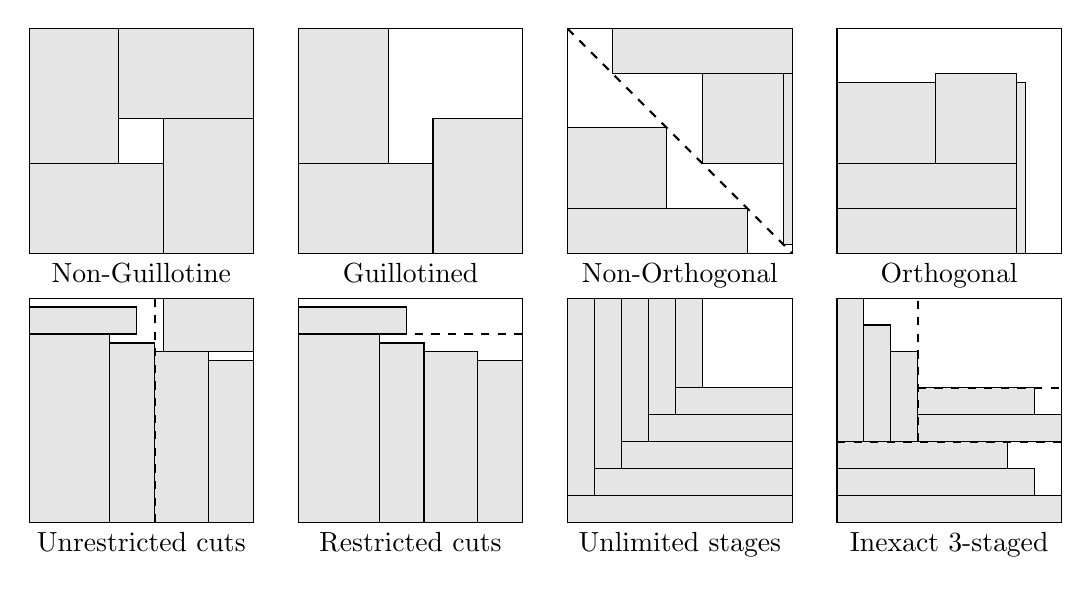
\begin{tikzpicture}[scale=0.114]
\def\piececolor{gray!20}
\def\labelxshift{12.5}
\def\labelyshift{0}
\def\labelfontsize{\normalsize}
\begin{scope}[shift={(0, 0)}] % FIRST ROW
\begin{scope}[shift={(0, 0)}] % FIRST IMAGE
\draw (0,0) rectangle +(25, 25);
\draw[fill=\piececolor] (0, 0) rectangle +(15, 10);
\draw[fill=\piececolor] (15, 0) rectangle +(10, 15);
\draw[fill=\piececolor] (0, 10) rectangle +(10, 15);
\draw[fill=\piececolor] (10, 15) rectangle +(15, 10);

\node [below] at (\labelxshift, \labelyshift) {\labelfontsize Non-Guillotine};
\end{scope}

\begin{scope}[shift={(30, 0)}] % SECOND IMAGE
\draw (0,0) rectangle +(25, 25);
\draw[fill=\piececolor] (0, 0) rectangle +(15, 10);
\draw[fill=\piececolor] (15, 0) rectangle +(10, 15);
\draw[fill=\piececolor] (0, 10) rectangle +(10, 15);
%\draw[fill=\piececolor] (10, 10) rectangle +(15, 10);

\node [below] at (\labelxshift, \labelyshift) {\labelfontsize Guillotined};
\end{scope}

\begin{scope}[shift={(60, 0)}] % THIRD IMAGE
\draw (0,0) rectangle +(25, 25);
\draw[fill=\piececolor] (0,0) rectangle +(20, 5);
\draw[fill=\piececolor] (0,5) rectangle +(11, 9);
\draw[fill=\piececolor] (5, 20) rectangle +(20, 5);
\draw[fill=\piececolor] (15, 10) rectangle +(9, 10);
\draw[fill=\piececolor] (24, 1) rectangle +(1, 19);

\draw[dashed, thick, black] (0, 25) -- (25, 0);

\node [below] at (\labelxshift, \labelyshift) {\labelfontsize Non-Orthogonal};
\end{scope}

\begin{scope}[shift={(90, 0)}] % FOURTH IMAGE
\draw (0,0) rectangle +(25, 25);
\draw[fill=\piececolor] (0,0) rectangle +(20, 5);
\draw[fill=\piececolor] (0, 10) rectangle +(11, 9);
\draw[fill=\piececolor] (0, 5) rectangle +(20, 5);
\draw[fill=\piececolor] (11, 10) rectangle +(9, 10);
\draw[fill=\piececolor] (20, 0) rectangle +(1, 19);

\node [below] at (\labelxshift, \labelyshift) {\labelfontsize Orthogonal};
\end{scope}
\end{scope}

\begin{scope}[shift={(0, -30)}] % SECOND2 ROW
\begin{scope}[shift={(0, 0)}] % FIRST IMAGE
\draw (0,0) rectangle +(25, 25);

%\draw[fill=\piececolor] (0,0) rectangle +(6, 19);
%\draw[fill=\piececolor] (6,0) rectangle +(5, 18);
\draw[fill=\piececolor] (14,0) rectangle +(6, 19);
\draw[fill=\piececolor] (20,0) rectangle +(5, 18);
\draw[fill=\piececolor] (0,0) rectangle +(9, 21);
\draw[fill=\piececolor] (9,0) rectangle +(5, 20);
%\draw[fill=\piececolor] (0,19) rectangle +(10, 6);
\draw[fill=\piececolor] (15,19) rectangle +(10, 6);
\draw[fill=\piececolor] (0,21) rectangle +(12, 3);

\draw[dashed, thick, black] (14, 0) -- (14, 25);

\node [below] at (\labelxshift, \labelyshift) {\labelfontsize Unrestricted cuts};
\end{scope}

\begin{scope}[shift={(30, 0)}] % SECOND IMAGE
\draw (0,0) rectangle +(25, 25);

%\draw[fill=\piececolor] (0,0) rectangle +(6, 19);
%\draw[fill=\piececolor] (6,0) rectangle +(5, 18);
\draw[fill=\piececolor] (14,0) rectangle +(6, 19);
\draw[fill=\piececolor] (20,0) rectangle +(5, 18);
\draw[fill=\piececolor] (0,0) rectangle +(9, 21);
\draw[fill=\piececolor] (9,0) rectangle +(5, 20);
%\draw[fill=\piececolor] (0,19) rectangle +(10, 6);
%\draw[fill=\piececolor] (15,19) rectangle +(10, 6);
\draw[fill=\piececolor] (0,21) rectangle +(12, 3);

\draw[dashed, thick, black] (0, 21) -- (25, 21);

\node [below] at (\labelxshift, \labelyshift) {\labelfontsize Restricted cuts};
\end{scope}

\begin{scope}[shift={(60, 0)}] % THIRD IMAGE
\draw (0,0) rectangle +(25, 25);

\draw[fill=\piececolor] (0,0) rectangle +(25, 3);
\draw[fill=\piececolor] (0,3) rectangle +(3, 22);
\draw[fill=\piececolor] (3,3) rectangle +(22, 3);
\draw[fill=\piececolor] (3,6) rectangle +(3, 19);
\draw[fill=\piececolor] (6,6) rectangle +(19, 3);
\draw[fill=\piececolor] (6,9) rectangle +(3, 16);
\draw[fill=\piececolor] (9,9) rectangle +(16, 3);
\draw[fill=\piececolor] (9,12) rectangle +(3, 13);
\draw[fill=\piececolor] (12,12) rectangle +(13, 3);
\draw[fill=\piececolor] (12,15) rectangle +(3, 10);

\node [below] at (\labelxshift, \labelyshift) {\labelfontsize Unlimited stages};
\end{scope}

\begin{scope}[shift={(90, 0)}] % FOURTH IMAGE
\draw (0,0) rectangle +(25, 25);
\draw[fill=\piececolor] (0,0) rectangle +(25, 3);
%\draw[fill=\piececolor] (0,3) rectangle +(3, 22);
\draw[fill=\piececolor] (0,3) rectangle +(22, 3);
%\draw[fill=\piececolor] (3,6) rectangle +(3, 19);
\draw[fill=\piececolor] (0,6) rectangle +(19, 3);

\draw[fill=\piececolor] (0,9) rectangle +(3, 16);
\draw[fill=\piececolor] (9,9) rectangle +(16, 3);
\draw[fill=\piececolor] (3,9) rectangle +(3, 13);
\draw[fill=\piececolor] (9,12) rectangle +(13, 3);
\draw[fill=\piececolor] (6,9) rectangle +(3, 10);

\draw[dashed, thick, black] (0, 9) -- (25, 9);
\draw[dashed, thick, black] (9, 9) -- (9, 25);
\draw[dashed, thick, black] (9, 15) -- (25, 15);

\node [below] at (\labelxshift, \labelyshift) {\labelfontsize Inexact 3-staged};
\end{scope}
\end{scope}
\end{tikzpicture}


  \legend{\justifying \newtext{In \emph{Non-Orthogonal}, \emph{Unrestricted cuts}, and \emph{Restricted cuts}, the dashed line indicate the first cut of the pattern. In \emph{Inexact 3-staged}, the dashed lines indicate the last cut of each stage. Consider this last diagram. The bottom three horizontal cuts are done in the first stage. In the second stage, two pieces from the first stage are trimmed by a vertical cut and the three leftmost vertical cuts are done. In the third stage, two of the three pieces of the second stage are trimmed with horizontal cuts and the two rightmost horizontal cuts are done. The fact the variant is inexact only matters for the topmost piece among the two pieces cut in the third stage; the vertical cut that trims that piece \emph{must} be done after the third stage and therefore happens at the trim-only fourth stage only allowed in a three-staged variant if it is \emph{inexact}. Souce: the author.}}
  \label{fig:qualifier_examples}
\end{figure}

The literature further distinguishes between \emph{weigthed} and \emph{unweighted} problem variants.
In the weighted variant, pieces have an arbitrary profit value, while in the unweighted variant, the profit value is always equivalent to the piece area.
Consequently, the unweighted variant is equivalent to minimising waste and is a particular case of the weighted variant.
Any algorithm that solves the weighted variant (as is the case in this thesis) can solve the unweighted variant by setting the piece profit values to their areas.

\section{Motivation}

\oldtext{The G2KP and its closely related variants are of undisputable interest of the industry, especially wood, paper, metal, and glass cutting industries.}
\newtext{Guillotine cutting problems are of interest of the industry, especially the wood~\cite{yanasse:linear:2008,morabito:hardboard:2007} and glass cutting industries~\cite{clautiaux:2019,parreno:2020}, often because of machinery limitations.}
\oldtext{The vast and growing literature on the subject examined by~\citet{iori:2020} and by~\citet{russo:2020} is enough proof of such interest.}
\newtext{There is a vast and growing literature on the subject as evidenced by~\citet{iori:2020} and by~\citet{russo:2020}.}
\oldtext{To pick a single recent case study see~\citet{clautiaux:2019}, which solves a unique variant of the Guillotine 2D Cutting Stock Problem for a glass factory manufacturing double-paned windows.}
\newtext{The cutting optimization problem proposed in the \emph{ROADEF/EURO Challenge 2018} was a guillotine cutting problem. The challenge was developed in collaboration with Saint-Gobain Glass France (a reference on flat glass manufacture). See~\citet{parreno:2020} for more details on this challenge.}

This work focuses on MILP as the solving method (instead of \emph{ad hoc} solutions) because its adaptability amplifies the value of any enhancements discovered.
A better MILP formulation means: a better solving procedure for the many (already mentioned) closely related problem variants;
a better continuous relaxation for computing an optimistic guess on the objective value of all these variants (some \emph{ad hoc} algorithms of the literature use MILP solvers to compute their bounds);
not only a better exact method but also a better base for heuristics or anytime procedures;
an immediate benefit from parallelisation, automatic problem decomposition, and solver-implemented heuristics;
and, finally, better ageing of the method over the years through the current trends of multiple-cores processors and ever-advancing solver performance.

\section{Contributions and thesis \oldtext{proposal} outline}
\label{sec:contributions}

\oldtext{
The main contributions of this work are:
an enhanced MILP formulation based on a previous state-of-the-art formulation, its proof of correctness, and empirical evidence of its better performance;
a straightforward adaptation of a previously known reduction procedure for both the original and the enhanced formulations, and empirical evidence of its positive impact on their performance;
new upper and lower bounds, as well as optimal values, for many recently proposed hard instances from~\citet{velasco:2019}.
For such, the author reimplemented a state-of-the-art MILP formulation and an optional pricing procedure used by it.
This reimplementation allows us to compare both approaches fully.
All code used is available in the first author's repository ({\small\url{https://github.com/henriquebecker91/GuillotineModels.jl/tree/0.2.4}}).}
% TODO: remove below only after we had put a similar disclaimer in each experiment section.
% \newtext{For reproducibility, the exact version of the code employed in this paper is available at~\cite{code:0:2:4}. However, we suggest using the better documented and maintained master branch ({\small\url{https://github.com/henriquebecker91/GuillotineModels.jl}}) if perfect reproduction is not necessary.}

\newtext{
The contributions of this thesis include:
\begin{itemize}
\item an enhanced MILP formulation based on a previous state-of-the-art formulation, its proof of correctness, and empirical evidence of its better performance;
\item a novel way to employ a previously known property (plate-size normalisation) for both the original and the enhanced formulations, and empirical evidence of its positive impact on their performance;
\item new upper and lower bounds, as well as optimal values, for many recently proposed hard instances from~\citet{velasco:2019};
\item a direct comparison with recent formulations of the literature highlighting the weak and strong points of each;
\item the adaptation of the proposed formulation for three related problems (G2MKP, G2OPP, and G2CSP) and empirical results over literature datasets to serve as base for future comparisons between formulations;
\item an hybridisation of the proposed formulation (with the formulation from~\citet{silva:2010}) that has moderate success in further reducing the run time for instances in which most time is spent at the B\&B phase (by disallowing some symmetries).
\end{itemize}
For such, the author reimplemented a state-of-the-art MILP formulation and an optional pricing procedure used by it.
}

The rest of the thesis is organised in the following way.
\Cref{sec:related_work} contextualises the topic of the thesis in the broader literature and lists the prior work on it.
\Cref{sec:tech_background} introduces the necessary mathematical concepts as well as the formulation used as the basis for the proposed formulation, the proposed formulation itself, and adaptations for the variant allowing rotation.
\Cref{sec:furini_vs_enhanced_comparison} experimentally examine the difference in model size and overall performance between the reimplementation of the base formulation, the original data on it, and the proposed (re-)formulation.
\Cref{sec:martin_chapter} experimentally examine the performance of the proposed formulation against other recent formulations of the literature for the G2KP.
\Cref{sec:other_problems} explains how to adapt the proposed formulation to three related problems and empirically test the adaptations over literature datasets; it also reports a generation mistake found in the T dataset.
\Cref{sec:hybridisation} presents an adaptation of the proposed formulation that hybridises it with a prior formulation for a more restricted problem without losing the optimality for the general case; experiments are included.
\Cref{sec:conclusions} delivers the conclusions based on the experiments presented in the previous chapters.
\Cref{sec:datasets} provides a detailed description of each instance dataset employed in this thesis.

\chapter{Related work}
\label{sec:related_work}

The literature on 2D cutting and packing, in general, is vast, as pointed out by \citet{iori:2020}, which catalogues exact methods and relaxations of \newtext{problems from} this field.
Even if the scope is further restricted to exact methods for the G2KP, the author could write a forty-page survey on it, as it was done by~\citet{russo:2020}.
Consequently, the author strongly suggests both surveys mentioned above for any reader interested in a broader understanding of the literature.

The review presented here is divided into two parts. The first part contextualises the reader by contraposing aspects of the thesis topic to other aspects found in the broader cutting and packing literature. The second part focus on the brief history of our main topic (i.e., MILP formulations for the G2KP).

\section{Broader literature contextualisation}

This section presents a list of aspects \textbf{not} shared by the thesis topic.
For each item, the literature concerning that aspect is briefly summarised.
If adequate, the item also contrasts the aspect with its opposite present in the main topic.

\subsection{Non-Guillotine\newtext{d problems}}

Both the G2KP and the 2KP are strongly NP-hard \citep{iori:2020}, and none is a generalisation of the other.
Therefore, theoretically, no problem is overall more challenging than the other.
In terms of modelling, however, the 2KP has the additional challenge that, once the first piece is cut, the remaining space is nonconvex \citep{fekete:1997}.
The G2KP has a better subproblem structure in this regard.
In the G2KP, once a cut is defined, there are two convex spaces, and the problem may be seen as multiple heterogeneous \newtext{G}2KPs\footnote{In fact, in the \cref{sec:adaptation_to_g2mkp} it will be shown that adapting the proposed formulation to the Multiple Knapsack Problem (homogeneous variant) is very straightforward because of this property.}.
However, this nicer structure cannot be fully exploited if a 2KP solving method is adapted to support guillotine cuts.
In \citet{nascimento:2019}, for example, the solving method has a harder time solving the G2KP because it is a method for the 2KP with the overhead of identifying guillotine cuts over it.

\subsection{Unconstrained \newtext{problems}}

The unconstrained G2KP was introduced by~\citet{gg:1965}, some mistakes of this first work were posteriorly corrected by~\citet{herz:1972}\footnote{\newtext{\citet{herz:1972} points out a mistake in an \emph{improved} algorithm presented in~\citet{gg:1965}. The improved algorithm reduces computational effort by skipping some horizontal and vertical cuts based on four criteria that should not impact the guarantee of optimality. A counterexample shows that this is not the case as the only optimal solution of the counterexample is unatainable when the four criteria are followed.}}
and by~\citet{beasley:1985:guillotine}\footnote{\newtext{\citet{beasley:1985:guillotine} points out a mistake in the \(k\)-staged recursion presented in~\citet{gg:1965}. In their recursion, the cut orientation of the first stage (either horizontal or vertical) changes depending on the current stage, e.g., the third stage assumes the first stage had vertical cuts, but the fourth stage assumes the first stage had horizontal cuts instead.}}.
Differently from the constrained variant, which is strongly NP-Hard, the unconstrained variant is weakly NP-Hard (it generalises the 1D Unbounded Knapsack Problem).
Consequently, exact solving methods in pseudo-polynomial time are possible, especially through Dynamic Programming (DP).
The lack of the combinatorial explosion caused by keeping track of the residual demand is what makes DP the most popular approach for the unconstrained variant and mostly unused for the constrained variant.
Such is the gap in difficulty between both variants that the state-of-the-art heuristic for the constrained variant solves the unconstrained variant repeatedly \citep{velasco:2019}.
The state-of-the-art method for the unconstrained problem appears to be \citet{russo:2014}, which is a DP method; they regarded the B\&B algorithm of \citet{kang:2011} as the previous state of the art.

\subsection{Heuristic \newtext{methods}}

As it is common for classic (strongly) NP-Hard problems, the literature on heuristic methods is colossal.
For example, \citet{ortmann:2010} compares across 252 heuristics for the 2D Strip Packing Problem (guillotine and non-guillotine variants).
For the thesis main problem, the G2KP, the author believes the best heuristic method is the one proposed by~\citet{velasco:2019}.
The method is inspired by the dynamic programming state-space relaxation of~\citet{nicos:1995:ssr}, which also inspired the earlier state-of-the-art heuristic that is~\citet{morabito:2010}.
The procedures described by \citet{velasco:2019} give both lower and upper bounds.
These methods were run over 500 instances of the literature for both rotation and no-rotation variants; they obtained either optimal or better bounds in all cases.
The bounds proved the optimality of 348 instances for the no-rotation variant and 385 for the rotation variant; some instances were open.
\citet{velasco:2019} then proposes 80 more challenging instances (which are included in this thesis experiments) and proves the optimality of many of them.

\subsection{Approximative \newtext{methods}}

For the G2KP, with and without rotation or weights, \citet{abed:2015} provide a quasi-Polynomial Time Approximation Scheme (quasi-PTAS), assuming the input data to be quasi-polynomially bounded integers (\citet{anna:2015:quasi} has a similar result for the non-guillotine variant).
For the Guillotine 2D Bin Packing Problem (without rotation), \citet{bansal:2005} gives an Asymptotic PTAS (APTAS).
\citet{christensen:2017} informs us that finding a PTAS for the Non-Guillotine 2D Knapsack Problem (with or without rotation or weights) is an open problem and that, for the non-guillotine variant, ``\citet{bansal:2009} gave a PTAS for the special case when the range of the profit-to-area ratio of the rectangles is bounded by a constant for both the cases with and without rotations'' and ``there is no FPTAS unless \(P = NP\), even for packing squares into squares \citep{leung:1990}.
"\citet{galvez:2017} propose a polynomial-time 1.89-approximation for the Non-Guillotine 2D Knapsack Problem\footnote{\citet{galvez:2017} defines the original plate as a square and the pieces as rectangles.
It is possible to employ lossless scaling of the plate and the pieces to, without changing the optimal value, transform the original plate of any problem instance into a square.
One downside is an increase in the absolute dimensions (i.e., precision).}, and a polynomial-time \(3/2 + \varepsilon\)-approximation for the rotation case, improved to a \(4/3 + \varepsilon\)-approximation if all piece profits are set to one.
These are the best results for the respective variants as far as the author knows.
For a survey on approximation algorithms for 2D cutting, the author refers to \citet{christensen:2017} and to \citet{iori:2020} (which briefly updates the former).

\subsection{Restricted \newtext{cuts}}

Considering only restricted cuts allows a simplified branching model: instead of having to consider a pseudo-polynomial number of horizontal and vertical cuts over each plate, only \(2n\) possibilities need to be considered, two for each piece, the one with the horizontal cut first, and the one with the vertical cut first (both generate the respective piece and up to two residual plates).
This exact branching model is employed by~\citet{silva:2010}.
For the unconstrained variant, \citet{song:2010}, proves a worst-case ratio of at least \(6/7\) between restricted and unrestricted optimal solutions for the same instance.
In contrast, \citet{furini:2016}, for the constrained variant, puts the ratio at most \(5/6\).
However, at least for the considered literature datasets, most instances have restricted and unrestricted optimal solutions of the same value.
The heuristic for the unconstrained variant described by \citet{song:2010} (which only employs restricted cuts) finds the unrestricted optimal value in ``94.84\%, 86.67\% and 77.83\% for small, medium and large sized unweighted instances'' and ``99.67\%, 99.50\% and 97.00\% for small, medium and large sized weighted instances''.
\citet{furini:2016} found that 47 of 50 instances, solved optimally by both restricted and unrestricted MILP models, shared the optimal solution value.

\subsection{Limited number of guillotine stages}

Unrestricted cuts are unnecessary to obtain any optimal solution of a two-staged variant (exact or non-exact), so the distinction between restricted and unrestricted two-staged variants do not exist.
For \(k\)-staged variants in which~\(k \geq 3\) there is such distinction, e.g., \citet{puchinger:2007} first models a formulation for the restricted three-staged G2CSP to then extend it to the unrestricted three-staged G2CSP.
For the unconstrained variant, and a small dataset, \citet{beasley:1985:guillotine} reported an average of about 0.4\% difference between the two-staged optimal value and the unlimited stages optimal value (about the same between two and three-staged, because three-staged is only 0.02\% behind unlimited stages).
For the constrained variant, however, \citet{martin:2020:models} presents an average difference of 3.6\% between two-staged and unlimited stages optimal solution values.
None of these papers poses this difference as a research question; these percentages are the byproduct of data gathered to answer other questions.
For the Guillotine 2D Bin Packing Problem, there is a theoretical result stating a two-staged optimal solution value may be at most 1.691 times worse than a solution with unlimited stages, but this is not a tight bound \citep{bansal:2005}.

\subsection{Exact but not pure MILP}

Besides solving methods with no relation to MILP models, this section also includes techniques that use MILP models but interleave their use with indispensable calls to non-MILP methods.
This section concentrates on works tackling the G2KP, and it is noted if another problem is considered instead.
The exact procedures observed here often fall into three categories: (i) branch-and-bound (or, as reported in the seminal works, \emph{tree search}); (ii) graph-based algorithms; (iii) repeated piece subset selections and packing tentatives.
The first category (i.e., B\&B) may be divided into top-down and bottom-up approaches.
Top-down approaches start from the original plate and branch on cuts over it and its subdivisions; this approach is probably the oldest one and is used in~\citet{cw:1977} and in~\citet{nicos:1995:ssr}.
Bottom-up approaches start from the pieces and combine them into builds, and the builds with each other, while they are smaller than the original plate.
This approach has many examples: \citet{bagchi:1993}, \citet{hifi:1997}, \citet{cung:2000}, and \citet{yoon:2013}.
The graph-based approaches include \citet{morabito:1996} and \citet{clautiaux:2018} (designed for four-staged but tested on unlimited stages, too); many previous papers by Clautiaux use graph representations for the G2OPP.

Finally, there are methods (often aided by MILP solvers) that solve a problem to select the most profitable subset of pieces, and then check if the subset can be guillotine-packed.
\citet{dolatabadi:2012} uses this approach, as did \citet{pisinger:2007}, but the latter focus on the G2CSP and the G2KP is solved just as a subproblem.
\citet{russo:2020} consider the methods of both \citet{dolatabadi:2012} and \citet{yoon:2013} to be state of the art, but the same work also points out that both methods have bounding flaws that may lead to incorrect results.

\newtext{Comprehensive counterexamples for the three bounding flaws found are given in the appendix of \citet{russo:2020}.
A brief overview of the roots of these three flaws follows.
The \emph{first two flaws} one in the antiredundancy strategy D1 of~\citet{cung:2000} and another in the unnamed strategy from~\citet{dolatabadi:2012} are, in essence, manifestations of the same oversight.
The oversight consists of restricting the search for an optimal solution to combinations of optimal solutions of subproblems (which are the same as the original problem but with the original plate dimensions reduced).
Such strategy is the basis of all dynamic programming and works flawlessly for the \emph{unconstrained} G2KP.
However, in the constrained case, a suboptimal solution to a subproblem may be necessary to assemble the optimal solution to the original problem.
A suboptimal solution for a subproblem may be necessary because, if an optimal solution for the subproblem were used instead, the combined solution would end up with more copies of some piece type than allowed by the piece demand, immediately becoming an invalid solution.
Removing pieces of the combined solution until the number of copies respects the demand does not (always) solve the problem; it is possible that the combination of two suboptimal solutions for the same subproblems would have a better value than this partially dismantled combination of optimal solutions.
The \emph{third flaw} was found in the works of~\citet{kang:2003,kang:2011,yoon:2013} and consists on a rounding problem.
Two formulae expressing upper bounds on the optimal solution value (i.e., optimal profit) have each two terms rounded down before they are summed.
\citet{russo:2020} presents a counterexample in which both \emph{upper} bounds give a result one unit \emph{lower} than the optimal solution value.
The bounds are valid if the rounding down only happens after the sum and not before it.
The method of~\citet{yoon:2013} also carries the flaw from~\citet{cung:2000}, which has affected other bottom-up methods in the literature too (see~\citet{russo:2020} for a complete overview).
%\emph{The first mistake} comes from a strategy employed by~\citet{dolatabadi:2012} and consists of only taking into account the best solution of a subproblem (the subproblem is the same problem but with a smaller original plate) when assembling the optimal solution for the main problem. This is a classic DP strategy and it works flawlessly for the unconstrained version of the problem. However, when applied to the constrained problem, it voids the guarantee of optimality because a suboptimal solution of a subproblem to be required, i.e., the optimal pattern of the subproblem cannot be repeated as many times as necessary in the main problem because of the demand constraints.
%\emph{The second mistake} comes from the antiredundancy strategy D1 from~\citet{cung:2000} and, again, it is related to discarding suboptimal subproblem solutions (and the subproblem is the problem with smaller original plate dimensions). The D1 strategy proposes that, when two subproblem solutions are combined, the result should be discarded if the dimensions of the merged solution clearly allow for an extra piece to be packed together with the pieces of both smaller solutions. The rationale for this strategy is that, as piece profits are always positive, the \emph{merged solution plus an extra piece that fits} will always have a better value for the same dimensions in comparison to the merge without the extra piece. However, again, the optimal pattern for the original problem may need the 
}
\oldtext{\citet{yoon:2013} flaw comes since \citet{cung:2000} and has affected other bottom-up methods too.}
Consequently, there is no clear definition of which is the best method currently.

\section{MILP formulations for the G2KP}

\citet{russo:2020}~identify three strategies employed by previous exact methods which cause loss of the optimality guarantee\newtext{, i.e., these methods cannot be considered exact anymore}.
No previous MILP formulation, nor this work, employs any of these strategies.
One of these strategies is a dominance rule valid for the unconstrained case but not for the constrained one.
Interestingly, \citet{herz:1972}~proposed a dominance rule for the unconstrained G2KP based on the same principle and warned about the possibility of misusing the rule in the constrained case.

The first MILP formulation dealing with guillotine cuts and unlimited stages was proposed by~\citet{messaoud:2008}.
The problem considered by~\citet{messaoud:2008} is the Strip Packing Problem\footnote{The Strip Packing Problem is a two-dimensional cutting/packing problem in which the pieces do not have profit values, and the original plate does not have a predefined length (`height' in the context of the problem); the objective is to minimize the height of the original plate while packing every piece.}, but adapting the formulation to the knapsack variant would not change its fundamentals.
Previously, \citet{lodi:2003}~had proposed two MILP formulations for two-staged G2KP.
As noted by~\citet{belov_thesis:2003}, modeling \(k\)-staged cuts for \(k \geq 3\) (unlimited stages included) was considered difficult at the time.
The size of most \(k\)-staged formulations is exponential on the number of stages (i.e.,~\(k\)).
The formulation of~\citet{messaoud:2008} had about \(3n^4/4\) variables and \(2n^4\) constraints (where \(n\) is the number of pieces); it also employed, according to the authors, a ``very loose linear relaxation'' due to which ``the practical interest of this formulation is still limited''.
The characterization of guillotine cuts proposed by~\citet{messaoud:2008} seems to have been simultaneously proposed by~\citet{pisinger:2007}. % This is the "Using decomposition" paper.

The first MILP formulation specifically for the G2KP was proposed by~\citet{furini:2016}.
\newtext{The formulation is classified as an extension of the one-cut formulation from~\citet{dyckhoff:1981} for the one-dimensional Cutting Stock Problem.
However, the formulation from~\citet{silva:2010} can be seen as an intermediary step between these two: it had already extended the one-cut formulation for two dimensions in a similar fashion but did not alter the problem from the cutting stock and was limited to two stages and restricted three stages.
} An extended version of~\citet{furini:2016} appears in~\citet{dimitri_thesis} (a PhD thesis)\newtext{, and a prelude to it in~\citet{furini:conference:2016}}.
Their formulation has pseudo-polynomial size, \(O((L + W) \times L \times W)\)~variables and \(O(L \times W)\) constraints, and its relaxation provides a stronger bound than~\citet{messaoud:2008}.
It was the first formulation able to solve medium-sized instances of the literature.
Besides the formulation, \citet{furini:2016}~proposes two reductions and one pricing procedure; these three are reimplemented in this work.
They also present and prove a theorem to assure the correctness of one of their reductions~(\emph{Cut-Position}).
A similar theorem and proof appear in~\citet{song:2010} but for the unconstrained variant.

In this work, the author proposes an enhanced formulation based on the formulation from~\citet{furini:2016} mentioned above.
A significant advantage of the enhancement is to avoid the enumeration of any cuts after the middle of a plate.
This advantage appears in many works since~\citet{herz:1972}.
Recently, \citet{delorme:2019} \oldtext{adapted}\newtext{enhanced} a \newtext{pseudo-polynomial} formulation for the 1D Cutting Stock Problem to obtain this same advantage.
However, the way \citet{delorme:2019}~changes their formulation to obtain this advantage is different from the approach taken here.
\newtext{The mechanisms involved in each approach are distinct.
\citet{delorme:2019} mechanism adds only a single reflecting dummy node per bin stock size to compensate for the removed arcs/variables, but it is meant for the 1D variant of the problem.
The mechanism proposed here adds a set of extraction variables in which the cardinality depends on the geometric properties of the specific instance considered, but it is meant for the 2D variant and also cuts down some symmetries that only exist in the 2D variant (i.e., are not present in the 1D variant).}

The most recent MILP formulations for the G2KP come from the following three works by Martin et alii:~\citet{martin:2020:models,martin:2020:bottom,martin:2020:top}.\oldtext{For the sake of conciseness, in this paragraph, we will refer to these three works as the \emph{Martin's works}, also we will refer to the formulation of~\citet{furini:2016} as the \emph{FMT formulation}.}\oldtext{The formulations in the Martin's works are compared against the FMT formulation.}\oldtext{We base our enhanced formulation on the FMT formulation and also compare against it.}\oldtext{The formulations in the Martin's works have a looser relaxation bound compared to the FMT formulation, but perform better than the FMT formulation in instances for which the FMT formulation has a much larger number of variables.}\oldtext{Considering the instances used in~\citet{furini:2016}, our enhanced formulation dominates the FMT formulation.}\oldtext{Our formulation also dramatically improves the running times of instances in which the FMT formulation performed worse than the ones from Martin's works (e.g., the gcut1--gcut12 instances).}\oldtext{Consequently, while it may be interesting for completeness sake, we do not compare against the formulations proposed in Martin's works in the current work.} \newtext{Besides the formulations from these three works, a previous formulation from \citet{martin:2019} targets the G2KP with defects (i.e., the original plate has regions that cannot be part of any piece).}
\newtext{A direct comparison between formulations with and without defects is unfair; modelling the defects burdens a formulation greatly.}
\newtext{Moreover, most formulations cannot be straightforwardly adapted to the G2KP with defects, including the one proposed in this work.}
\newtext{However, the results may be interpreted not as a direct comparison, but as an assessment of the impact of modelling defects over a formulation.}
\newtext{These four formulations are discussed in details in~\cref{sec:martin_chapter} in which they participate in experiments.}

% We discuss the related works in the topic of cut position discretisation in the following section.
% The topic demands more notation and connects with the reduction we adapt from the previous literature for our enhanced formulation.

% TODO: Should all words in the title be capitalized?
% TODO: Is this title ok? maybe Normalizing Plate Size?
\chapter{Technical background and the proposed formulation}
\label{sec:tech_background}

This chapter introduces all the technical details necessary to contextualize the proposed formulation and the formulation itself.
Outside of this chapter, the proposed formulation (also referred to as the enhanced formulation) will also be referred to as BBA (Becker, Buriol, and Araújo) as to follow the same naming convention applied to FMT (Furini, Malaguti, and Thomopulos) from~\citet{furini:2016}.
\Cref{sec:psn} introduces notation for the chosen discretisation, discusses some alternative discretisations, outlines the cut-and-plate enumeration procedure, and dives deeply into the known (but innovatively employed) plate-size normalisation.
\Cref{sec:furini_model} summarises the formulation proposed in~\citet{furini:2016}, which is the basis for the formulation proposed by this thesis and gives it an intuitive interpretation.
\Cref{sec:enhanced_model} describes the proposed formulation, how it differs from its basis, and intuition for why the changes (generally) lead to a performance improvement.
\Cref{sec:proof_of_correctness} presents a proof for the claim that the proposed formulation can find a cutting pattern for any multiset of pieces for which the original formulation also finds a cutting pattern, this is, that the guarantee of optimality is retained.
\Cref{sec:adaptation_for_rotation} shows how both discussed formulations can be adapted to allow piece rotation and \cref{sec:mirror_plate} shows a reduction that is specific to those formulations with rotation enabled.
Finally, \cref{sec:pricing} presents a summary of the pricing procedure employed in~\citet{furini:2016} and reimplemented by the author for the experiments of this thesis.

\section{Notation, Discretisation, and Plate-Size Normalisation}
\label{sec:psn}

The performance of solving methods for cutting and packing problems often heavily depends on the number of cut/packing positions considered.
Since the seminal works of~\citet{cw:1977} and~\citet{herz:1972}, solving methods avoid considering each possible position but instead consider only a subset necessary to guarantee optimality.
The literature includes many such subsets, which are often referred to as \emph{discretisations}.
The most common way of computing these discretisations is Dynamic Programming (DP) algorithms.
These DP algorithms usually only take a small fraction of the running time, but the size of the position subset outputted by them strongly affects the time spent by the rest of the solving method.

Both the proposed formulation and its basis have one constraint for each attainable distinctly-sized plate and one variable for each potential cut over each of these plates.
Therefore, eliminating a single cutting position has the following effects:
\textbf{(i)} it removes one variable for each distinctly-sized plate that allowed that cutting position;
\textbf{(ii)} if that cutting position was the only way to produce some distinctly-sized plates\footnote{Note that the same cutting position, when applied to distinctly-sized plates, may generate different children.}, then it also removes the constraints associated with these plates;
\textbf{(iii)} if (ii) excludes one or more constraints/plates, then it also excludes all variables representing possible cuts over the excluded plates;
\textbf{(iv)} finally, if (iii) eliminates one or more variables/cuts, then it may trigger (ii) again (i.e., other plates stop being attainable), cyclically.

In this work, the only cut subset (discretisation) considered are the canonical dissections of~\citet{herz:1972}, hereafter referred to as \emph{normal cuts} instead.
The author acknowledges the existence of stricter discretizations: the raster points of~\citet{terno:1987,guntram:1966}, the regular normal patterns of~\citet{boschetti:2002} (named this way by~\citet{cote:2018}), and the Meet-in-the-Middle (MiM) of~\citet{cote:2018}.
The reasons for the author's choice of discretisation are numerous: it works well with the \emph{Plate-Size Normalisation} procedure described in the sequence; it is the same discretisation employed by Furini's formulation (from which the proposed formulation is based on);\oldtext{MiM main gain}\newtext{The main gain of MiM} is reducing the number of cut positions after the middle of a plate, which the enhanced formulation already discards anyway; the regular normal patterns compute a distinct subset-sum for each pair of plate and piece, which the author considers excessive (there may exist hundreds of thousands of intermediary plate possibilities); finally, the raster points complicate the proofs presented here and the \emph{Plate-Size Normalisation} weakens its benefits.

\oldtext{The set~\(O = \{v, h\}\) denotes the cut orientation: \(v\) is vertical (parallel to width, perpendicular to length); \(h\) is horizontal (parallel to length, perpedicular to width).}
\newtext{The set~\(O = \{h, v\}\) denotes the cut orientation: \(h\) is horizontal (parallel to width, perpendicular to length); \(v\) is vertical (parallel to length, perpedicular to width).}
Let us recall that the demand of a piece~\(i \in \bar{J}\) is denoted by~\(u_i\).
By defining the set of pieces fitting a plate~\(j\) as~\(I_j = \{i \in \bar{J} : l_i \leq l_j \land w_i \leq w_j \}\), the set \(N_{jo}\) (i.e., the set of the normal cuts of orientation~\(o\) over plate~\(j\)) can be defined as:

{\iffinalversion\else\color{blue}\fi
\begin{equation}
N_{jo}= \left\{
\begin{array}{lllr}
  \{q: 0 < q < l_j; & \exists n_i \in [0 \isep u_i], \forall i \in I_j, q = \sum_{i\in I_j} n_i l_i \} & \quad \text{if } o = h,\\
  \{q: 0 < q < w_j; & \exists n_i \in [0 \isep u_i], \forall i \in I_j, q = \sum_{i\in I_j} n_i w_i \} & \quad \text{if } o = v.
\end{array}\right.
\end{equation}
}

The sets defined above never include cuts at the plate extremities (i.e., \(0\), \(l_j\) for \oldtext{\(N_{j_v}\)}\newtext{\(N_{jh}\)}, and \(w_j\) for \oldtext{\(N_{jh}\)}\newtext{\(N_{jv}\)}).
Any of these cuts will always create (i)~a~zero-area plate and (ii)~a~copy of the plate that is being cut.
Consequently, these cuts only add symmetries and may be disregarded.

\newtext{
The set \(J\) can now be defined by the following procedure: the original plate (plate~\(0\)) is added to \(J\), then for every plate~\(j \in J\) every cut in~\(N_{jv} \cup N_{jh}\) is applied to~\(j\), and each child generated is added to \(J\) if it can fit at least one piece.
The process finishes when every plate in~\(J\) was considered for cutting, and no new plates were generated.
Such procedure guarantees each piece~\(i \in \bar{J}\) will always be present in~\(J\) unless the piece does not fit the original plate (in which case it is irrelevant to the problem and could be removed a priori).
}

The goal of the \emph{Plate-Size Normalisation} procedure propose here is to reduce the number of distinctly-sized plates considered.
Fewer distinctly-sized plates mean fewer constraints and trigger the same cascading effect described by items (ii)--(iv) above.
The property exploited by the procedure is already known and \oldtext{similarly} exploited by~\citet{alvarez:2009} and by~\citet{dolatabadi:2012}.
The author chose to state the property the following way:

\begin{proposition}
\label{pro:normalisation}
% Without loss of optimality, plate~\(j\) may always be replaced by plate~\(j\prime\) with \(w_{j\prime} = w_j\) but \(l_{j\prime} = max\{q : q \in N_{kv}, q \leq l_j\}\) in which \(w_k = w_j\) but \(l_k > l_j\).
Given a plate~\(j \in J\), \(l_j\) may always be replaced by \(l^\prime_j = max\{q : q \in N_{kh}, q \leq l_j\}\) in which \(k \in J\), \(w_k = w_j\), but \(l_k > l_j\), without loss of optimality.
The analogue is valid for the width.
\end{proposition}

\newtext{In other words, if increasing the length (width) of plate~\(j\) reveals that the original length (width) did not match a normal cut position in the enlarged plate, then plate~\(j\) may be replaced by a shorter plate in which the length (width) is reduced to the largest normal cut position smaller than the original length (width). For example, given \(l = [5, 7]\), \(w = [3, 2]\), a 13x3 plate may be reduced to 12x3 (13 does not match a normal cut while \(5 + 7 = 12\) does), and a 13x2 plate may be reduced to 7x2 (13 does not match a normal cut while 7 does).}
No proof is replicated here. The following can now be defined:

\begin{definition}{Size-normalised plate}
The length of a plate~\(j\) is considered normalised if, and only if, \(l_j = l^\prime_j\).
The analogue is valid for the width.
The size of a plate is normalised if, and only if, both its length and its width are normalised.
\end{definition}

The \emph{Plate-Size Normalisation} procedure proposed here consists only of replacing every non-size-normalised plate enumerated by its normalised counterpart.
\newtext{In summary, every intermediary plate \emph{for which the length (width) is not a linear combination of the length (width) of the pieces} have its dimensions reduced to the closest linear combination smaller than itself; this combines multiple plate types that could only pack the same set of pieces into a single plate type.
}\oldtext{The number of distinctly-sized plates diminishes because the procedure replaces many plates of distinct but similar dimensions by a single plate.
}The only extra effort added by \emph{Plate-Size Normalisation} consists of binary searches over~\(N_{jo}\) sets for each plate~\(j\)\newtext{, and these may be carried out without increasing the overall complexity, given the setup of~\(O(LW)\) vectors of size \(O(L + W)\); a setup step which also does not increase the overall complexity.
However, in the implementation, the author opted to increase the overall complexity from \(O(L^2W + LW^2)\) to \(O(L^2Wlog(L) + LW^2log(W))\) because the fraction of time spent on the enumeration was not enough to justify the memory and code complexity trade-off.
In practice, even if the worst-case complexity increases, the time spent decreases because the actual number of plates (denoted in the complexity by~\(O(LW)\) becomes more distant from the worst-case}.
A suitable \(N_{ko}\) set for each plate~\(j\) was already computed by the plate enumeration procedure before introducing the \emph{Plate-Size Normalisation} (no extra effort required).

\begin{remark}
\oldtext{If a normal cut~\(q\) divides the size-normalised plate~\(j\), the first child is always size normalised, but the second child may not be size normalised.}
\newtext{If a normal cut divides a size-normalised plate, then the dimension perpendicular to the cut, in the first child, is normalised. The dimension parallel to the cut in the first child, and both dimensions of the second child, are not guaranteed to be normalised.}
\end{remark}

% The concept of normal cuts is introduced by
% Every optimal solution with non-normal cuts can be mapped to an optimal solution only using normal cuts.
% The definition used here is almost the same of~\citet{furini:2016}, as we are trying to keep our notation compatible with theirs.

% TODO: the definitions below need the definition of orientation.
% TODO: define the sizes set `S_{oj}` where? "given vertical cuts are parallel to length and horizontal cuts parallel to width, we define the size set ..."
% TODO: define Q_{jo} here, like in furini:2016, maybe change paragraph above to say we will be using the same definition of furini:2016

% is the set of pieces that fit plate~\(j\).
%\(O = \{v, h\}\) defines both vertical and horizontal orientations.
%Considering that vertical is parallel to length, and horizontal is parallel to width, we can use them to index plate sizes as in~\(S_{jv} = l_j\) and \(S_{jh} = w_j\).
%Allowing us to define normal cuts as:

%\begin{definition}
%\(Q_{jo} = \{ 0 < q < S_{oj}; \forall i \in I_j, \exists n_i \in \mathbb{N}, n_i \leq u_i, q = \sum_{i\in I_j n_i S_{oi}}\}\)
%\end{definition}

% Let us denote the \emph{original plate} as plate~\(0\).
% Every cut c in Q_{0o} define a plate with a side of size S_{0o} and another of size S_{co}

% The \emph{plate-size normalisation} works by replacing groups of plates (with similar but distinct size) by a single plate.
% If there exists a plate~\(j : S_{oj} > max\{N_{oj}\}\) then \(j\) may be replaced by a plate~\(k : S_{ok} = max\{N_{oj}\}\).

%In this section, we prove that no valid solution is lost if plate dimensions are shortened to a discretisation point.
%For convenience, we denote the set of pieces that fit a plate~\(j\) by \(\bar{J}_j\); a piece~\(i\) fits a plate~\(j\) iff \(l_i \leq L_j \land w_i \leq W_j\).%, and that plates cut from a shortened plate may need additional shortening after the cut.

%\begin{definition}
%The set of pieces that fit a plate~\(j\) is denoted by \(\bar{J}_j\), a piece~\(i\) fit a plate~\(j\) if \(l_i \leq L_j \land w_i \leq W_j\).
%\end{definition}

%\begin{definition}
%The set of horizontal normal cuts of a plate~\(j\) is the set of all non-trivial linear combinations \(\sum_{i \in \bar{J}_j} a_i \times l_i \leq L\) for which the coefficients \(a_i\) are restricted by \(0 \leq a_i \leq u_i~\forall.~i \in \bar{J}_j\). The analogue is valid for vertical cuts.
%\end{definition}

%In~\citet{cw:1977}, \emph{normal cuts} are defined for the variant of the problem without the demand constraints.
%Our definition of normal cuts is extended to take into consideration the demand.
%The following theorem and its proof (provided in \cref{app:proof_only_normal_cuts_needed}) are also extensions to account for the demand.
%We also extend a theorem, and its proof, that restricting the cuts to (our definition of) normal cuts allows packing any demand-abiding piece mulstiset that could be packed with non-normal cuts.
%We also extend a theorem, and its proof, that restricting the cuts to (our definition of) normal cuts allows packing any demand-abiding piece mulstiset that could be packed with non-normal cuts.

%\begin{theorem}\label{only_normal_cuts_needed}
%For every guillotine packing with non-normal cuts packing a set of pieces~\(s\), there is a guillotine packing of only normal cuts packing the largest subset of~\(s\) that respects the demand.
%producing the same pieces or, if the former packing produced an amount exceeding the demand for some piece type, the latter paproduces the maximum amount allowed by the demand for such piece types.
%\end{theorem}

%is in the appendix, as similar proofs are presented in the literature.

%\begin{corollary}\label{co:size_normalised_plate}
%Given a plate~\(j\) in which the right (or top) border do not overlap with the rightmost vertical (or topmost horizontal) normal cut, any demand-abiding piece multiset packed in~\(j\) can be packed in its size-normalised alternative, in which the plate size is reduced until the borders overlap with normal cuts.
%\end{corollary}

%\begin{proof}
%The proof of the~\cref{only_normal_cuts_needed} describes an alternative packing with the property that any space between the rightmost vertical cut and the plate right border (topmost horizontal cut and the plate top border) is waste. Therefore, if a plate is replaced by its size-normalised alternative, no used space would be lost, and no packing would be invalid.\qed
%\end{proof}

%\begin{remark}
%If a size-normalised plate is cut by a normal cut, the first child is also size-normalised. The second child, however, may or may not be size-normalised.
%\end{remark}

%In the dimension parallel to the cut, the border of the first child will overlap with the normal cut applyed to the parent plate; on the other dimension, the border already overlapped a normal cut.

\begin{example}{Denormalisation after normalised cut}\label{ex:renormalisation_after_cut}
\oldtext{Given two pieces with \(l = [5, 7]\), \(u = [2, 3]\), and a size-normalised plate of length~\(21\), a normal cut at~\(12\) creates a non-normalised second child of length~ \(9\).}
\newtext{Consider three pieces with~\(l = [5, 7, 9]\), \(w = [6, 4, 11]\), \(u = [3, 1, 1]\), and a plate of dimensions \(15\)x\(15\). The plate dimensions are already normalised. The plate length matches stacking the three copies of the first piece. The plate width matches the other two pieces lying side-by-side. An horizontal cut at length~\(7\) is a normal cut because it matches the length of the second piece. If the cut is done, the width of both children is not normalised anymore, nor is the length of the second child. The width of both children is not normalised because the third piece does not fit either child so, for both children, the largest width a valid packing may reach is~\(12\). The length of the second child is not normalised because the largest length a valid packing inside the second child may reach is 7. The dimensions of both children may be normalised to \(7\)x\(12\). This example already shows an immediate gain: instead of creating two new plate sizes, the enumeration only creates a single new plate type. The cut creates two copies of this single type of plate.}
\end{example}

\begin{figure}[h]
  \caption{\newtext{Diagram of Example~\ref{ex:renormalisation_after_cut}}}
  \center
  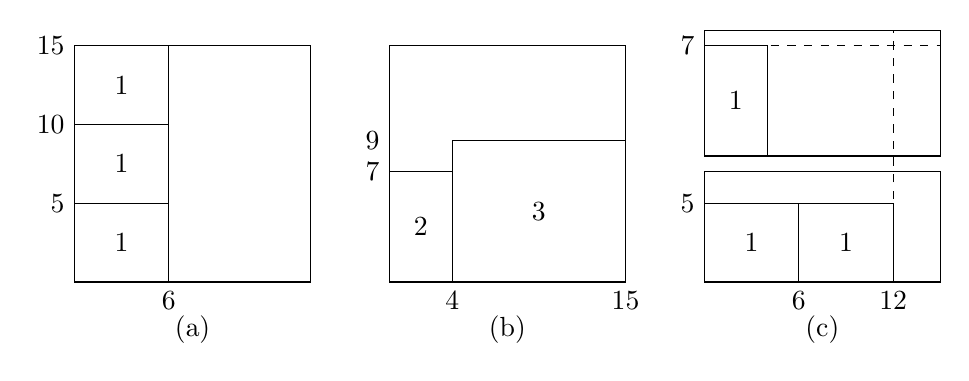
\begin{tikzpicture}[scale=0.20]
\begin{scope}[shift={(0, 0)}]
\draw [draw=black]   (0, 0) rectangle ++(15, 15);
\draw [draw=black]   (0, 0) rectangle     ++(6, 5) node [midway] {1};
\draw [draw=black]   (0, 5) rectangle     ++(6, 5) node [midway] {1};
\draw [draw=black] (0, 10) rectangle     ++(6, 5) node [midway] {1};
\node [left]  at (0, 5) {5};
\node [left]  at (0, 10) {10};
\node [left]  at (0, 15) {15};
\node [below]  at (6, 0) {6};
\node [below] at (7.5, -1.5) {(a)};
\end{scope}
\begin{scope}[shift={(20, 0)}]
\draw [draw=black]   (0, 0) rectangle ++(15, 15);
\draw [draw=black]   (0, 0) rectangle     ++(4, 7) node [midway] {2};
\draw [draw=black]   (4, 0) rectangle   ++(11, 9) node [midway] {3};
\node [below]  at   (4, 0)   {4};
\node [below]  at (15, 0) {15};
\node     [left]  at   (0, 7)   {7};
\node   [left]  at (0, 9)   {9};
\node [below] at (7.5, -1.5) {(b)};
\end{scope}
\begin{scope}[shift={(40, 0)}]
\draw [draw=black]   (0, 0) rectangle ++(15, 7);
\draw [draw=black]   (0, 0) rectangle     ++(6, 5) node [midway] {1};
\draw [draw=black]   (6, 0) rectangle     ++(6, 5) node [midway] {1};
\node [left]  at (0, 5) {5};
\node [below]  at (6, 0) {6};
\node [below]  at (12, 0) {12};
\draw[dashed] (12, 0) -- (12, 16);

\draw [draw=black]   (0, 8) rectangle ++(15, 8);
\draw [draw=black]   (0, 8) rectangle   ++(4, 7) node [midway] {1};

\node     [left]  at   (0, 15)   {7};
\draw [dashed] (0, 15) -- (15, 15);
\node [below] at (7.5, -1.5) {(c)};
\end{scope}
\end{tikzpicture}


  \legend{\justifying \newtext{Notes about the diagrams: (a) the three copies of the first piece stacked; (b) the second and third pieces side-by-side; (c) both children of an horizontal normal cut over a normalised plate are not normalised themselves.}}
  \label{fig:renormalisation_after_cut}
\end{figure}

\newtext{
While the basic property (\cref{pro:normalisation}) is well known by the literature, some of the developments given here are not.
Generally, in the literature, the procedure is employed a single time just for the original plate, and \emph{not} for every plate generated during an enumeration procedure like it is done here.
Because the procedure is commonly applied once, the denormalisation effect mentioned here is not studied or discussed.
Also, applying the procedure a single time often is done to get a better relaxation, which is not the case for the proposed formulation.
In the proposed formulation and its basis, the dimensions are abstracted by a flow graph connecting cuts and plates; the dimensions are not right-hand values of binding constraints.
The plate-size normalisation does not affect the relaxation; instead, it reduces the model size because multiple intermediary plate types are conflated into a single type.
}

%%%%%%%%%%%%%%%%%%%%% SECTION BREAK %%%%%%%%%%%%%%%%%%%%%

\section{\newtext{The FMT formulation and associated reductions}}
\label{sec:furini_model}

Given pseudo-polynomial time and space, an instance of the G2KP can be transformed into a bipartite directed acyclic (multi)graph; solving a flow-like problem over such graph is equivalent to solving the original G2KP instance.
The two disjoint and independent sets of vertices are (i) the enumerated plate types and (ii) the enumerated cuts over the plate types.
Each cut vertice has one incoming edge and one or two outgoing edges.
The head of the incoming edge is the plate vertice that represents the plate being cut.
The tail of each outgoing edge is a plate vertice representing a plate produced by the cut.
These are all edges that exist in the graph.
If the cut vertice has only two incident edges, it represents a trim cut, i.e., a cut that only reduces the size of an existing plate without producing a second plate.
If the cut vertice has three incident edges, it represents a plate cut into two smaller plates.
As the graph is a multigraph, it allows for parallel edges, representing a cut exactly at the middle of a plate generating two copies of the same plate type.

The aforementioned flow-like problem is as follows.
All edges only allow integer amounts to flow between vertices.
The vertice representing the original plate type is the only one to start with one flow unit (all other vertices start zeroed).
If a plate vertice receives any flow amount, it can keep any portion of the flow in the vertice and freely redistribute the remaining flow among its outgoing edges.
If a cut vertice receives any flow amount, it \emph{multiplies} the amount of flow received by the number of outgoing edges, and \emph{must} relay the exact amount of flow received to \emph{each} of the outgoing edges, e.g., if a cut vertice receives two units of flow then each outgoing edge receives two units of flow.
If a plate vertice represents a plate type of the same dimensions as a piece~\(i\), then each unit of flow kept by the vertice generates a profit~\(p_i\) constrained to a maximum of~\(u_i \times p_i\).
The problem is deciding how the plate vertices will distribute the flow they receive to maximize said profit.

The formulation proposed in~\citet{furini:2016}, henceforth referred to as the FMT formulation, generates models similar to the graph described and which are solved similarly to the flow-like problem mentioned.
As previously defined, the set \(O = \{h, v\}\) denotes the horizontal and vertical cut orientations.
The set \(Q_{jo}\) (\(\forall j \in J, o \in O\)) denotes the set of possible cuts (or cut positions) of orientation~\(o\) over plate~\(j\).
\newtext{The set \(Q_{jo}\) is not formally defined because it is a subset of~\(N_{jo}\) (formally defined in the last section) that varies based on which reductions are being applied.}

The parameter~\(a\) is a byproduct of the plate enumeration process and represents the edges of the graph.
\oldtext{The value of \(a^o_{qkj}\) is the number of plates \(j \in J\) added to the stock if a cut of orientation~\(o \in O\) is carried out at position~\(q \in Q_{jo}\) of a plate~\(k \in J\).}
\newtext{The value of~\(a^o_{qkj}\) indicates how many copies of a plate~\(j \in J\) are produced by cutting a plate~\(k \in J\) with a cut of orientation~\(o \in O\) at position~\(q \in Q_{ko}\).}
This value may be zero (no plate created by the cut has the same dimensions as \(j\), i.e., no edge exists), one (one plate created by the cut has the same dimensions as \(j\), i.e., there is an edge), or two (the parent plate was cut in half, and both halves have the same dimensions as \(j\), i.e., two parallel edges).
This parameter is needed to write the constraints that control which plates are available.
The description of this parameter in~\citet{furini:2016} has a typo, as pointed out by~\citet{martin:2020}:``[...] there is a typo in their definition of parameter~\(a^o_{qkj}\), as the indices~\(j\) and~\(k\) seem to be exchanged.''.
The original parameter description also forgets the possibility that it may have value two (instead of just zero and one).

In a valid solution, the value of \(x^o_{qj}\) is the number of times a plate~\(j \in J\) is cut with orientation~\(o \in O\) at position~\(q \in Q_{jo}\); i.e., how much flow is being transported by each edge coming from a plate vertice.
The plate~\(0 \in J\) is the original plate, and it may also be in~\(\bar{J}\), as there may exist a piece of the same size as the original plate.
The \(y_i\) variable denotes the number of times a plate~\(i\) was sold as the piece~\(i\) (as \(\bar{J} \subseteq J\), each index~\(i \in \bar{J}\) denote both a piece and the plate of the exact same dimensions).

% Formulation version without the \specialcell workaround below.
% The problem with the formulation formatting is that the first restriction is
% too long before the quantifiers, and the penultimate restriction is too
% long in the quantifiers, so making them two distinct columns with align
% breaks the layout (and send the equation reference numbers of each line
% to an empty line below the). The workaround is some dark magic that flushes
% the quantifiers to right, instead of giving them their own shared column.
%\begin{align}
%\mbox{max.} &\sum_{(i, j) \in E} p_i e_{ij} \label{eq:objfun}\\
%\mbox{s.t.} &\sum_{o \in O}\sum_{q \in Q_{jo}} x^o_{qj} + \sum_{i \in E_{*j}} e_{ij} \leq \sum_{k \in J}\sum_{o \in O}\sum_{q \in Q_{ko}} a^o_{qkj} x^o_{qk} \hspace*{0.05\textwidth} & \forall j \in J, j \neq 0,\label{eq:plates_conservation}\\
%	& \sum_{o \in O}\sum_{q \in Q_{0o}} x^o_{q0} + \sum_{i \in E_{*0}} e_{i0} \leq 1 &,\label{eq:just_one_original_plate}\\
%	& \sum_{j \in E_{i*}} e_{ij} \leq u_i & \forall i \in \bar{J},\label{eq:demand_limit}\\
%% TODO: fix equation below, the forall part is too long and clashes with the long equation in the first line
%	& x^o_{qj} \in \mathbb{N}^0 & \forall j \in J, o \in O, q \in Q_{jo},\label{eq:trivial_x}\\
%	& e_{ij} \in \mathbb{N}^0 & \forall (i, j) \in E.\label{eq:trivial_e}
%\end{align}

\begin{align}
\bm{max.} &\sum_{i \in \bar{J}} p_i y_i \label{eq:FMT_objfun}\\
\bm{s.t.} &\specialcell{\sum_{o \in O}\sum_{q \in Q_{jo}} x^o_{qj} \leq \sum_{k \in J}\sum_{o \in O}\sum_{q \in Q_{ko}} a^o_{qkj} x^o_{qk} \hspace*{0.05\textwidth} \forall j \in J\setminus\bar{J}, j \neq 0,}\label{eq:FMT_plates_conservation}\\
            &\specialcell{y_i + \sum_{o \in O}\sum_{q \in Q_{io}} x^o_{qi} \leq \sum_{k \in J}\sum_{o \in O}\sum_{q \in Q_{ko}} a^o_{qki} x^o_{qk} \hspace*{0.05\textwidth} \forall i \in \bar{J}, i \neq 0,}\label{eq:FMT_plates_conservation_and_sale}\\
	    &\specialcell{\sum_{i \in \{i | i \in \bar{J} \land w_i = w_0 \land l_i = l_0\}} y_i + \sum_{o \in O}\sum_{q \in Q_{0o}} x^o_{q0} \leq 1 \hspace*{\fill},}\label{eq:FMT_just_one_original_plate}\\
            & \specialcell{y_i \leq u_i \hspace*{\fill} \forall i \in \bar{J},}\label{eq:FMT_demand_limit}\\
	    & \specialcell{x^o_{qj} \in \mathbb{N}^0 \hspace*{\fill} \forall j \in J, o \in O, q \in Q_{jo},}\label{eq:FMT_trivial_x}\\
            & \specialcell{y_i \in \mathbb{N}^0 \hspace*{\fill} \forall i \in \bar{J}.}\label{eq:trivial_y}
\end{align}

The objective function maximizes the profit of the plates sold as pieces~\eqref{eq:FMT_objfun}.
Constraints~\eqref{eq:FMT_plates_conservation} and~\eqref{eq:FMT_plates_conservation_and_sale} guarantee that for every intermediary plate~\(j\) that was further cut (left-hand side), or plate/piece~\(i\) that was either sold or further cut (left-hand side), there must be a cut making available a copy of such plate (right-hand sides).
One copy of the original plate is available from the start~\eqref{eq:FMT_just_one_original_plate}, and it can be either sold as a piece of the same dimensions or further cut.
The amount of sold copies of some piece type must respect the demand for that piece type~\eqref{eq:FMT_demand_limit}.
Finally, the domain of all variables is the non-negative integers~\eqref{eq:FMT_trivial_x}-\eqref{eq:trivial_y}.

\newtext{
Besides the base formulation, \citet{furini:2016}~also employs a basic symmetry-breaking strategy and proposes two reductions for the model size.
The cut enumeration in~\citet{furini:2016} excludes one of each pair of perfectly symmetrical cuts.
Perfectly symmetrical cuts are pairs of cuts that create the same set of two child plates (i.e., just which is the first and which is the second that is reversed).
\citet{furini:2016} chose to ignore the symmetric cut in the second half of the plate during the enumeration.
The \emph{Cut-Position} reduction confines the set of cutting positions over some plates to the restricted set.
The condition for a plate to be affected by Cut-Position is that it should be able to pack \emph{at most} five pieces because, in such case, its restricted and unrestricted optimal value are the same (see \cref{fig:distinctions_restricted_unrestricted}).
The \emph{Redundant-Cut} reduction only removes a subset of the \emph{trim cuts}, i.e., cuts in which the second child plate is immediately considered waste because it is smaller than every piece.
Redundant-Cut removes a trim cut over plate~\(j\), which obtains plate~\(j^\prime\), if plate~\(j\) itself can \emph{only} be obtained by trim cuts of the same orientation from larger plates.
The rationale is that these larger plates can directly obtain~\(j^\prime\) through a single trim cut instead of using~\(j\) as an intermediary plate.
This way, the reduction removes unnecessary intermediaries and avoids the many symmetric patterns that only vary on the number of trim cuts employed to reduce a larger plate down to \(j^\prime\).
}
%%%%%%%%%%%%%%%%%%%%% SECTION BREAK %%%%%%%%%%%%%%%%%%%%%

\section{The proposed (re-)formulation}
\label{sec:enhanced_model}

\oldtext{EDIT NOTE: this section was called ``Changes to Furini's model'' before.}

The FMT is elegant: the pieces are just intermediary plates that may be sold.
The proposed changes affect both the enumeration step and the formulation mathematical description.
These changes significantly reduce the model size.
However, these changes also deepen the distinction between plates and pieces and may be regarded as sacrificing some elegance for performance.
The essentials of the formulation remain the same, but the proposed formulation has better performance in the vast majority of the problem instances.
For this reason, the author considers the formulation proposed here as an enhanced iteration of the FMT.
In general, the relaxation of the proposed model is the same as the FMT.

% TODO: should we say that this supersedes the furini original symm-breaking
% and their redundant-cut reduction?

As mentioned at the end of the last section, FMT allows for removing one of each pair of perfectly symmetrical cuts (which can be arbitrarily chosen to be the one in the second half of the plate).
Differently,~\citet{cw:1977} disregards \emph{all} cuts after the middle of the plate because of symmetry.
If FMT did the same as~\citet{cw:1977}, it could become impossible to trim a plate to the size of a piece.
For example, if there was a piece with a length larger than half the length of a plate, and such plate has no normal cut with the exact length of the needed trim, then the piece could not be extracted from the plate, even if the piece fits into the plate.
The goal of the proposed formulation is to reduce the number of cuts (i.e., model variables) by getting closer to the symmetry-breaking rule used in~\citet{cw:1977} without loss of optimality.
\newtext{Of course, disregarding every cut after the midplate also insulates against any perfectly symmetrical cuts and, therefore, supersedes a check just for this specific kind of symmetry.}
%First we present our changes to the formulation and the variable enumeration, then we prove the model correctness is not affected.

Considering the graph representation for FMT presented in the last section, it can be said that the proposed formulation throws away the possibility of piece-sized plate vertices to convert flow into profit and creates a third disjoint and independent set of vertices representing the pieces.
The vertices of this new set are all leaves/sinks responsible for converting flow to the corresponding piece profit.
The edges that reach the new vertices always come from plate vertices, but the plates do not need to have the exact dimensions of the pieces anymore.
These edges work as a shortcut to trimming, and multiple vertice plates may have an edge pointing to the same piece vertice as well as each vertice plate may have edges to multiple piece vertices.
This change alone leads to a larger model; however, as the edges to this new set of vertices allow us to obtain pieces without needing trim cuts, the symmetry-breaking strategy can be expanded to consider every cut after the middle of a plate.
This reduction leads to far fewer edges, as the cut position discretisation is often denser in the second half of the plate (compared to the first half).
It also means fewer plate vertices, as many plates were only necessary as intermediary steps to trimming a plate to the size of a piece.

%Often, there are many more normal cuts in the second half of a plate than there is in the first half. % need explanation?
%Also, if all cuts that generated some plate type are disregarded, then every cut over such plate type is also disregarded.
%Taking all of this into account, the main purpose of our revised version of Furini's formulation is to improve its symmetry breaking. % TODO: This has also the effect of superseding the Redundant-Cut reduction, which EXPLAIN SUCCINTLY THE REDUNDANT CUT.

\subsection{Changes to the formulation description}
\label{sec:enhanced}

The changes to the formulation are restricted to replacing the set of integer variables~\(y_i, i \in \bar{J},\) with a new set of variables~\(e_{ij}, (i, j) \in E, E \subseteq \bar{J} \times J\), and the necessary adaptations to accomodate this change.
In FMT, \(y_i\) denotes the number of times a plate~\(i\) was sold as the piece~\(i\) (plate~\(i\) has the exact same dimensions as piece~\(i\)).
The \emph{extraction variables}~\(e_{ij}\) denote a piece~\(i\) was extracted from plate~\(j\) which dimensions may only be the same or larger than the piece~\(i\) dimensions.
The exact definition of set~\(E\) is discussed over~\cref{sec:var_enum}; for the purpose of presenting the formulation, the intuitive definition of~\(e_{ij}\) just above is enough.
For convenience, the following are defined: \(E_{i*} = \{ j : \exists~(i, j) \in E \}\) and \(E_{*j} = \{i : \exists~(i, j) \in E \}\).
The variables \(x^o_{qj}\) and coefficients \(a^o_{qkj}\) have the same meaning as the FMT formulation (\cref{sec:furini_model}).

% Formulation version without the \specialcell workaround below.
% The problem with the formulation formatting is that the first restriction is
% too long before the quantifiers, and the penultimate restriction is too
% long in the quantifiers, so making them two distinct columns with align
% breaks the layout (and send the equation reference numbers of each line
% to an empty line below the). The workaround is some dark magic that flushes
% the quantifiers to right, instead of giving them their own shared column.
%\begin{align}
%\mbox{max.} &\sum_{(i, j) \in E} p_i e_{ij} \label{eq:objfun}\\
%\mbox{s.t.} &\sum_{o \in O}\sum_{q \in Q_{jo}} x^o_{qj} + \sum_{i \in E_{*j}} e_{ij} \leq \sum_{k \in J}\sum_{o \in O}\sum_{q \in Q_{ko}} a^o_{qkj} x^o_{qk} \hspace*{0.05\textwidth} & \forall j \in J, j \neq 0,\label{eq:plates_conservation}\\
%	& \sum_{o \in O}\sum_{q \in Q_{0o}} x^o_{q0} + \sum_{i \in E_{*0}} e_{i0} \leq 1 &,\label{eq:just_one_original_plate}\\
%	& \sum_{j \in E_{i*}} e_{ij} \leq u_i & \forall i \in \bar{J},\label{eq:demand_limit}\\
%% TODO: fix equation below, the forall part is too long and clashes with the long equation in the first line
%	& x^o_{qj} \in \mathbb{N}^0 & \forall j \in J, o \in O, q \in Q_{jo},\label{eq:trivial_x}\\
%	& e_{ij} \in \mathbb{N}^0 & \forall (i, j) \in E.\label{eq:trivial_e}
%\end{align}

\begin{align}
\bm{max.} &\sum_{(i, j) \in E} p_i e_{ij} \label{eq:objfun}\\
\bm{s.t.} &\specialcell{\sum_{o \in O}\sum_{q \in Q_{jo}} x^o_{qj} + \sum_{i \in E_{*j}} e_{ij} \leq \sum_{k \in J}\sum_{o \in O}\sum_{q \in Q_{ko}} a^o_{qkj} x^o_{qk} \hspace*{0.05\textwidth} \forall j \in J, j \neq 0,}\label{eq:plates_conservation}\\
%            & \specialcell{\sum_{o \in O}\sum_{q \in Q_{jo}} x^o_{qj} \leq \sum_{k \in J}\sum_{o \in O}\sum_{q \in Q_{ko}} a^o_{qkj} x^o_{qk} \hspace*{\fill} \forall j \in J\setminus\bar{J},}\label{eq:generic_plates_conservation}\\
	    & \specialcell{\sum_{o \in O}\sum_{q \in Q_{0o}} x^o_{q0} + \sum_{i \in E_{*0}} e_{i0} \leq 1 \hspace*{\fill},}\label{eq:just_one_original_plate}\\
            & \specialcell{\sum_{j \in E_{i*}} e_{ij} \leq u_i \hspace*{\fill} \forall i \in \bar{J},}\label{eq:demand_limit}\\
	    % TODO: fix equation below, the forall part is too long and clashes with the long equation in the first line
	    & \specialcell{x^o_{qj} \in \mathbb{N}^0 \hspace*{\fill} \forall j \in J, o \in O, q \in Q_{jo},}\label{eq:trivial_x}\\
            & \specialcell{e_{ij} \in \mathbb{N}^0 \hspace*{\fill} \forall (i, j) \in E.}\label{eq:trivial_e}
\end{align}

The objective function maximizes the profit of the extracted pieces~\eqref{eq:objfun}.
Constraint~\eqref{eq:plates_conservation} guarantees that for every plate~\(j\) that was further cut or had a piece extracted from it (left-hand side), there must be a cut making available a copy of such plate (right-hand side).
One copy of the original plate is available from the start~\eqref{eq:FMT_just_one_original_plate}, and it can be either have a piece directly extracted or be further cut.
The amount of extracted copies of some piece type must respect the demand for that piece type (a piece extracted is a piece sold)~\eqref{eq:demand_limit}.
Finally, the domain of all variables is the non-negative integers~\eqref{eq:trivial_x}-\eqref{eq:trivial_e}.

\subsection{Changes to the cut-and-plate enumeration}
\label{sec:var_enum}

As mentioned in~\cref{sec:furini_model}, the FMT was proposed together with some mechanisms to reduce the model size: removing perfectly symmetrical cuts, \emph{Cut-Position}, and \emph{Redundant-Cut}.
\oldtext{The two last rules are not discussed here; \citet{furini:2016}~proves their correctness, and they do not conflict with the enhanced model.}
\newtext{Cut-Position does not conflict with the proposed formulation and can be employed alongside it to further reduce the model size.
The symmetry-breaking and Redundant-Cut are superseded in the proposed formulation.
Redundant-Cut eliminates a subset of the trim cuts from the formulation; however, the proposed formulation does not have trim cuts like those removed by Redundant-Cut because the extraction variables make them unnecessary.
%If the cuts can only happen before the midplate, then either (i) there is a cut before the midplate for which the associated piece(s) would also fit into the second half, or (ii) there are no cuts before the midplate and any piece larger than half the plate dimension is obtained utilizing extraction variables.
}

The use of the \(x\)~variables does not change from the original formulation to the revised formulation -- however, the size of the enumerated set of variables changes.
The revised enumeration does not create any variable~\(x^o_{jq}\) in which \((o = h~\land~q > \lceil w_j / 2 \rceil) \lor (o = v~\land~q > \lceil l_j / 2 \rceil)\).
%given that \(D^h_j \equiv W_j\) and \(D^v_j \equiv L_j\).

The original formulation has variables~\(y_i\), \(i \in \bar{J}\), while the revised formulation replaces them with variables~\(e_{ij}\), \((i, j) \in E\), \(E \subseteq \bar{J} \times J\).
Set~\(\bar{J} \times J\) is orders of magnitude larger than~\(\bar{J}\).
Consequently, set~\(E\) must be a small subset to avoid having a revised model with more variables than the original.
A suitable subset may be obtained by a simple rule: \((i, j) \in E\) if, and only if, packing piece~\(i\) in plate~\(j\) does not allow any other piece to be packed in~\(j\).
The reason this restricted subset is enough to keep the model correctness is presented in next section.

\newtext{
For the enhanced formulation to have more variables than the original formulation, \(|E| > |\bar{J}| + |\{x^o_{jq} : j \in J \land o \in O \land q \in Q_{jo} \land (o = h \land q > \lceil w_j / 2 \rceil) \lor (o = v \land q > \lceil l_j / 2 \rceil)\}|\) must hold, this is, the number of extraction variables must be larger than the number of pieces plus the sum of the number of cuts after the middle of each enumerated plate.
Unfortunately, there is no closed formula for these sets (except \(\bar{J}\) which is given), what makes necessary to compute the full enumeration to verify the difference.
}

%If an extra piece could be packed, then there is a normal cut that creates both a plate that may be used for this extra piece and a plate that may be used to pack~\(i\).
%So the idea here is to do the extraction as late as possible: if the piece may be extracted from a descendant, then the plate may be cut until this descendant is generated to then have the piece extracted from it.

\section{The proof of correctness}
\label{sec:proof_of_correctness}

The previous section presented a detailed explanation of the changes to the formulation and variable enumeration.
This section proves such changes do not affect the correctness of the model.
\oldtext{In \citet{furini:2016} (and, consequently, in their formulation), only the perfect symmetries described below are removed}.
\newtext{The core of the proof consists in showing that any piece multiset that can be \emph{packed} in some plate by the FMT formulation can also be packed by the enhanced formulation.
So, below, what is meant by saying that \emph{a plate can pack a piece multiset} is both (i) that the FMT and the enhanced formulation can represent a valid sequence of cuts obtaining such pieces from a plate but also that (ii) there is a solution for the decision problem variant of G2KP with the plate and the piece multiset as its inputs.
Both meanings are essentially the same because both formulations are exact and will find a solution if it exists.}
The changes \newtext{to FMT} may be summarized to:

\begin{enumerate}
\item There is no variable for any cut that occurs after the middle of a plate.
\item A piece may be obtained from a plate if, and only if, the piece \oldtext{fits}\newtext{is the same size or smaller than} the plate, and the plate cannot \oldtext{fit}\newtext{pack} an extra piece (of any type). \newtext{Obtaining a piece from a plate is always regarded as an extraction and not a cut.}.
\end{enumerate}

The second change alone cannot affect the correctness of the model.
The original formulation was even more restrictive in this aspect: a piece could only be sold if a plate of the same dimensions existed.
In the revised formulation, an extraction variable will always exist in such a case because, if a piece and plate match perfectly, there is no space for any other piece, fulfilling the only criteria for the existence of extraction variables.
Consequently, what needs to be proved is that:

\begin{theorem}{Piece extractions supersede all cuts after the middle of a plate.}

Without changing the pieces obtained from a \oldtext{packing}\newtext{plate}, any normal cut after the middle of a plate may be replaced by a combination of piece extractions and cuts at the middle of a plate or before it.
\label{the:enhanced_correctness}
\end{theorem}

\newtext{
As mentioned before, normal guillotine cuts can be used to search for a solution (in contrast to considering a cut at every position) without loss of optimality.
So the proof goes in the direction of showing that everything that can be done with normal guillotine cuts can be done without the normal cuts after the midplate but by allowing piece extractions.
The theorem above and the proof below assume a plate cannot be cut twice.
If a single cut is applied to a plate, then two new plates are created, and these may be further cut.
There is no loss of generality by undertaking this assumption, which is already implicitly undertaken in the rest of this work.
This difference can be seen as the same difference between the representation of the packing with a binary tree instead of a tree with a variable number of children.
}

\begin{proof} This is a proof by exhaustion. The set of all normal cuts after the middle of a plate may be split into the following cases:
\begin{enumerate}
  \item The cut has a perfect symmetry. \label{case:perfectly_symmetric}
  \item The cut does not have a perfect symmetry.
  \begin{enumerate}
    \item Its second child can \oldtext{fit}\newtext{pack} at least one piece. \label{case:usable_second_child}
    \item Its second child cannot \oldtext{fit}\newtext{pack} a single piece.
    \begin{enumerate}
      \item Its first child packs no pieces. \label{case:no_pieces}
      \item Its first child packs a single piece. \label{case:one_piece} % call luffy to help
      \item Its first child packs two or more pieces. \label{case:many_pieces}
    \end{enumerate}
  \end{enumerate}
\end{enumerate}

The author believes to be self-evident that the union of~\cref{case:perfectly_symmetric,case:usable_second_child,case:no_pieces,case:one_piece,case:many_pieces} is equal to the set of all normal cuts after the middle of a plate. An individual proof for each of these cases is presented below.

\begin{description}
\item[\Cref{case:perfectly_symmetric} -- \textbf{The cut has a perfect symmetry.}]
\oldtext{If two distinct cuts have the same children (with the only difference being the first child of one cut is the second child of the other cut, and vice-versa), then the cuts are perfectly symmetric.}
\newtext{Two horizontal (vertical) cuts over the same plate are considered \emph{perfectly symmetrical} if they generate the same children plate; for example, an horizontal cut at position five of a plate of length 15 creates the same two children (of lengths five and 10) than a cut at position 10.}
Whether a plate is the first or second child of a cut does not make any difference for the formulation or for the problem.
If the cut is in the second half of the plate, then its symmetry is in the first half of the plate.
Consequently, both cuts are interchangeable, and the one after the midplate may be dismissed.
\item[\Cref{case:usable_second_child} -- \textbf{Its second child can \oldtext{fit}\newtext{pack} at least one piece.}]
\Cref{pro:normalisation} allows us to replace the second child with a size-normalised plate that can pack any demand-abiding set of pieces the original second child could pack.
The second child of a cut that happens after the middle of the plate is smaller than half a plate, and its size-normalised counterpart may only be the same size or smaller.
So the size-normalised plate could be cut as the first child by a normal cut in the first half of the plate.
Moreover, the old first child (now second child) has stayed the same size or grown (because of the size-normalisation of its sibling), which guarantees this is possible.

\item[\Cref{case:no_pieces} -- \textbf{Its first child packs no piece.}]
If both children of a single cut do not pack any pieces, then the cut may be safely ignored.
\item[\Cref{case:one_piece} -- \textbf{Its first child packs a single piece.}]
First, let us ignore this cut for a moment and consider the plate being cut by it (i.e., the parent plate).
The parent plate either: can \oldtext{fit}\newtext{pack} an extra piece together with the piece the first child would pack, or cannot \oldtext{fit}\newtext{pack} any extra pieces.
If it cannot \oldtext{fit}\newtext{pack} any extra pieces, this fulfils the criteria for having an extraction variable, and the piece may be obtained through it.
The cut in question can then be disregarded (i.e., replaced by the use of such extraction variable).
However, if it is possible to \oldtext{fit}\newtext{pack} another piece, then there is a normal cut in the first half of the plate that would separate the two pieces, and such cut may be used to shorten the plate.
This kind of normal cuts may successively shorten the plate until it is impossible to pack another piece, and the single piece that was originally packed in the first child may then be obtained by employing an extraction variable.
\item[\Cref{case:many_pieces} -- \textbf{Its first child packs two or more pieces.}]
If the first child packs two or more pieces, but the second child cannot \oldtext{fit}\newtext{pack} a single piece (i.e., it is waste), then the cut separating the first and second child may be omitted and any cuts separating pieces inside the first child may still be done.
If some of the plates obtained by such cuts need the trimming that was provided by the omitted cut, then these plates will be packing a single piece each, and they are already considered in~\cref{case:one_piece}.
\end{description}

Given the cases cover every cut after the middle of a plate, and each case has a proof, then follows that \cref{the:enhanced_correctness} is correct.

\end{proof}


\begin{figure}[ht]
  \caption{\newtext{Visual help for the proof of correctness}}
  \center
  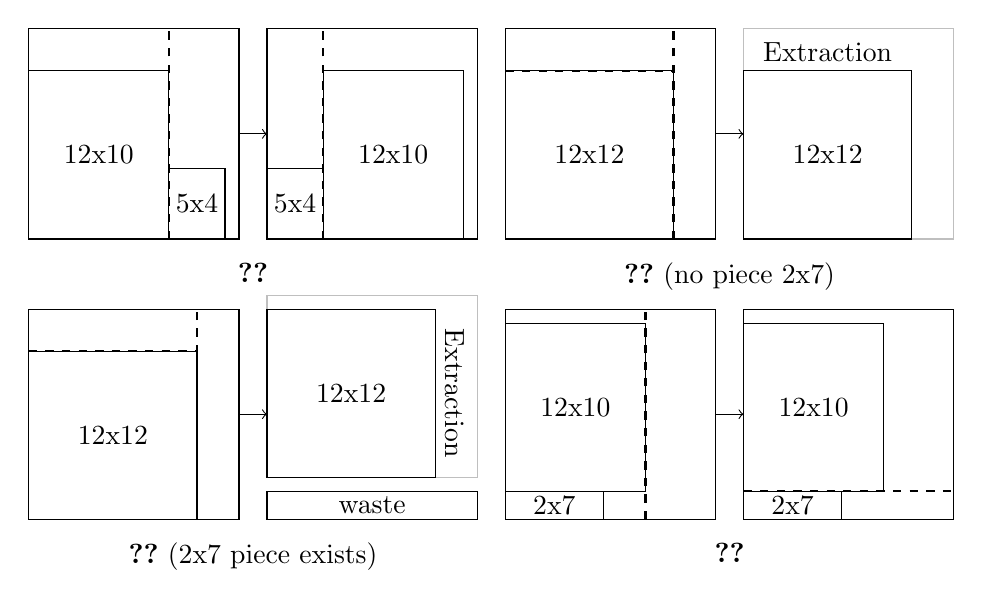
\begin{tikzpicture}[scale=0.178]
\def\piececolor{gray!20}
\def\labelxshift{16}
\def\labelyshift{-1}
\def\labelfontsize{\normalsize}
\def\innerlabelfontsize{\normalsize}
\def\extractioncolor{gray!50}
\begin{scope}[shift={(0, 0)}] % FIRST ROW
\begin{scope}[shift={(0, 0)}] % FIRST PAIR
\begin{scope}[shift={(0, 0)}] % FIRST IMAGE
\draw (0,0) rectangle +(15, 15);
\draw (0, 0) rectangle +(10, 12) node [midway] {\innerlabelfontsize 12x10};
\draw (10, 0) rectangle +(4, 5) node [midway] {\innerlabelfontsize 5x4};

\draw[dashed, thick, black] (10, 0) -- (10, 15);
\draw [-to](15, 7.5) -- (17,7.5);
\end{scope} % FIRST IMAGE

\begin{scope}[shift={(17, 0)}] % SECOND IMAGE
\draw (0,0) rectangle +(15, 15);
\draw (4, 0) rectangle +(10, 12) node [midway] {\innerlabelfontsize 12x10};
\draw (0, 0) rectangle +(4, 5) node [midway] {\innerlabelfontsize 5x4};

\draw[dashed, thick, black] (4, 0) -- (4, 15);
\end{scope} % SECOND IMAGE

\node [below] at (\labelxshift, \labelyshift) {\labelfontsize \Cref{case:usable_second_child}};
\end{scope} % FIRST PAIR


\begin{scope}[shift={(34, 0)}] % SECOND PAIR
\begin{scope}[shift={(0, 0)}] % FIRST IMAGE
\draw (0,0) rectangle +(15, 15);
\draw (0, 0) rectangle +(12, 12) node [midway] {\innerlabelfontsize 12x12};

\draw[dashed, thick, black] (12, 0) -- (12, 15);
\draw[dashed, thick, black] (0, 12) -- (12, 12);
\draw [-to](15, 7.5) -- (17,7.5);
\end{scope} % FIRST IMAGE

\begin{scope}[shift={(17, 0)}] % SECOND IMAGE
\draw[draw=gray!50] (0,0) rectangle +(15, 15);
\node [above] at (6, 12) {\labelfontsize Extraction};
\draw (0, 0) rectangle +(12, 12) node [midway] {\innerlabelfontsize 12x12};
\end{scope} % SECOND IMAGE

\node [below] at (\labelxshift, \labelyshift) {\labelfontsize \Cref{case:one_piece} (no piece 2x7)};
\end{scope} % SECOND PAIR
\end{scope} % FIRST ROW



\begin{scope}[shift={(0, -20)}] % SECOND ROW
\begin{scope}[shift={(0, 0)}] % FIRST PAIR
\begin{scope}[shift={(0, 0)}] % FIRST IMAGE
\draw (0,0) rectangle +(15, 15);
\draw (0, 0) rectangle +(12, 12) node [midway] {\innerlabelfontsize 12x12};

\draw[dashed, thick, black] (12, 0) -- (12, 15);
\draw[dashed, thick, black] (0, 12) -- (12, 12);
\draw [-to](15, 7.5) -- (17,7.5);
\end{scope} % FIRST IMAGE

\begin{scope}[shift={(17, 0)}] % SECOND IMAGE
\node [rotate=-90, above] at (12, 9) {\labelfontsize Extraction};
\draw[draw=\extractioncolor] (0, 3) rectangle +(15, 13);

\draw (0, 0) rectangle +(15, 2) node [midway] {waste};

\draw (0, 3) rectangle +(12, 12) node [midway] {\innerlabelfontsize 12x12};
\end{scope} % SECOND IMAGE

\node [below] at (\labelxshift, \labelyshift) {\labelfontsize \Cref{case:one_piece} (2x7 piece exists)};
\end{scope} % FIRST PAIR


\begin{scope}[shift={(34, 0)}] % SECOND PAIR
\begin{scope}[shift={(0, 0)}] % FIRST IMAGE
\draw (0,0) rectangle +(15, 15);
\draw (0, 0) rectangle +(7, 2) node [midway] {\innerlabelfontsize 2x7};
\draw (0, 2) rectangle +(10, 12) node [midway] {\innerlabelfontsize 12x10};

\draw[dashed, thick, black] (10, 0) -- (10, 15);
\draw [-to](15, 7.5) -- (17,7.5);
\end{scope} % FIRST IMAGE

\begin{scope}[shift={(17, 0)}] % SECOND IMAGE
\draw (0,0) rectangle +(15, 15);
\draw (0, 0) rectangle +(7, 2) node [midway] {\innerlabelfontsize 2x7};
\draw (0, 2) rectangle +(10, 12) node [midway] {\innerlabelfontsize 12x10};

\draw[dashed, thick, black] (0, 2) -- (15, 2);

\end{scope} % SECOND IMAGE

\node [below] at (\labelxshift, \labelyshift) {\labelfontsize \Cref{case:many_pieces}};

\end{scope} % SECOND PAIR

\end{scope} % SECOND ROW

\end{tikzpicture}

  \vspace{3mm}
  \legend{\justifying \newtext{\Cref{the:enhanced_correctness} case examples. \Cref{case:perfectly_symmetric,case:no_pieces} are excluded given their simplicity. In all examples, the parent plate is 15x15. In the example of~\cref{case:usable_second_child}, the cut would happen after the middle of the plate, but then the pieces of the second child can be packed in the first child instead. In the example of~\cref{case:one_piece}, both cuts happen after the middle of the plate, and there are no other pieces; however, as no piece may be extracted from the leftovers, then there is an extraction variable available. In the example of~\cref{case:one_piece}, a 2x7 piece exists, but it is not extracted from the plate (the demand for it may be exhausted, for example); therefore, the extraction variable from the previous case does not exist; however, the 2x7 piece allows us to make a cut just to reduce the plate length and, for the size of the second child, an extraction variable is available. Finally, in the example of~\cref{case:many_pieces}, which cut that happens first may be changed, as there is no piece packed in the subplate that would originally become the second child.}}
  \label{fig:proof_examples}
\end{figure}

\newtext{
\Cref{fig:proof_examples} may help the reader to visualize the more complicated parts of the proof.
From the cases above, the FMT formulation (from \citet{furini:2016}) only treats specially the pairs of cuts that are perfectly symmetrical to each other (by removing one of them).
}

\section{\newtext{Adaptation to the rotation variant}}
\label{sec:adaptation_for_rotation}

The adaptation of both FMT and the proposed formulation to the rotation-allowed variant of G2KP are very similar, and the author chose to employ only the proposed formulation to illustrate the process.
The changes needed are:

\begin{enumerate}
\item change the piece set~\(\bar{J}\) before the call to the enumeration procedure;\label{item:J_change}
\item create a new set~\(P\), which binds the two rotations of every piece;\label{item:P_creation}
\item change the constraint~\eqref{eq:demand_limit} to take into account this new set~\(P\).\label{item:demand_con_change}
\end{enumerate}

The changes mentioned in \cref{item:J_change} consist of adding to \(\bar{J}\) a new piece~\(i^\prime\) for each piece~\(i\) for which~\(\nexists k \in \bar{J} : l_k = w_i~\land~w_k = l_i\), piece~\(i^\prime\) have~\(l_{i^\prime} = w_i\), \(w_{i^\prime} = l_i\), and~\(u_{i^\prime} = u_i\); differently, for each piece~\(i\) for which~\(\exists k \in \bar{J} : l_k = w_i~\land~w_k = l_i\) (i.e., for each piece~\(i\) that has its rotation as an already existing piece~\(k\)), both \(u_i\) and \(u_k\) become the sum of their original values (given by the instance).

The set~\(P\) mentioned in~\cref{item:P_creation} may be defined as \(P = \{ \{i, k\} \in P : i \in \bar{J}, k \in \bar{J},  l_k = w_i~\land~w_k = l_i\}\). Each element of~\(P\) is a set of two pieces.

Finally, as mentioned in~\cref{item:demand_con_change}, the following change is made:

\begin{flalign*}
&& \sum_{j \in E_{i*}} e_{ij} \leq u_i && \forall i \in \bar{J}\tag{\ref{eq:demand_limit}}
%\specialcell{\sum_{j \in E_{i*}} e_{ij} \leq u_i \hspace*{\fill} \forall i \in \bar{J},}\tag{\ref{eq:demand_limit}}
\end{flalign*}

to

\begin{flalign}
&& \sum_{j \in E_{i*}} e_{ij} + \sum_{j \in E_{k*}} e_{kj} \leq u_i && \forall \{i, k\} \in P\label{eq:rotation_demand}
\end{flalign}

\section{\newtext{The rotation-specific mirror plate enhancement}}
\label{sec:mirror_plate}

The previous section describes only the minimal changes necessary to adapt the proposed formulation for the rotation-allowed variant.
This section describes a reduction for the formulation that is only possible if rotation is allowed.
This change is also compatible with the FMT formulation.

The core idea of the enhancement is that, if all pieces can rotate, then any two plates~\(j\) and~\(j^\prime\), for which \(l_j = w_{j^\prime} \land w_j = l_{j^\prime}\) holds, are equivalent to each other.
The rationale is simple: if a set of pieces is extracted from plate~\(j\) through a guillotine cutting pattern, then there exists an equivalent guillotine pattern in which every piece is rotated and which can be extracted from plate~\(j^\prime\) which is the rotation of plate~\(j\).
This way, if the cut and plate enumeration generates such plates~\(j\) and \(j^\prime\), only one of them needs to be kept (but every cut that generated the removed plate needs now to generate the kept rotation instead).
Finally, the opposite statement is also true (yet very inefficient): if all \emph{plates} could somehow rotate, then the pieces themselves would not need to be able to rotate, and distinct piece types that are rotations of each other could be considered the same.

The modifications necessary for the reduction are restricted to the cut-and-plate enumeration.
Only plates in which the length is smaller than the width are allowed.
If a cut would generate a plate with its length greater than its width, then the cut instead creates the rotated version of the plate, in which the length is the smallest dimension.
This change can potentially reduce the number of plates (constraints) to half their original amount.
Consequently, the number of variables (cuts and extractions over specific plate types) may also reduce up to half their original amount.

The only downside of mirroring the plates is that the Redundant-Cut reduction needs to be either disabled or adapted.
If plate mirroring is enabled, then Redundant-Cut needs to keep track if either (or both) child plates of a cut were rotated or not.
This tracking usually is not necessary to implement just the plate mirroring itself.
The experiments employing rotation focus mostly on the proposed formulation (in which Redundant-Cut is already disabled because it is superseded); the few experiments with rotation-enabled FMT have Redundant-Cut disabled.

\section{\newtext{The pricing phase}}
\label{sec:pricing}

The pricing procedure described in~\citet{furini:2016,dimitri_thesis} was reimplemented by us.
]No significant changes were made to the procedure.
As the experiments include multiple comparisons involving this procedure, a summary of the procedure is presented below.
For simplicity, the procedure takes an already built model (from either the original formulation or the enhanced version), and any previous reductions mentioned were already applied.
\citet{clautiaux:2018} refers to a similar procedure (that they apply to their own formulation) as \emph{lagrangian filtering}; however, this term is not employed by~\citet{furini:2016,dimitri_thesis}.

\begin{enumerate}
\item Fix to zero all variables representing horizontal (vertical) cuts that do not match a piece length (width).
\item Remove all integrality constraints and solve the relaxed model to obtain an upper bound for the position-only restricted problem.
\item Obtain a lower bound from an \emph{inexact 2-staged} heuristic~\citep{furini:2016,dolatabadi:2012}.\label{it:heuristic}
\item Employ the reduced costs of the model variables, the position-only restricted upper bound, and the heuristic lower bound to price-out variables (more details below) by fixing them to zero.\label{it:restricted_final_pricing}
\item Restore the integrality constraints, warm-start with the heuristic solution from (step \autoref{it:heuristic}), solve the model (currently, a reduced MILP model for the position-only restricted variant of the problem) and obtain a probably better lower bound. While unlikely, the heuristic may have already provided an optimal solution for the position-only restricted problem.\label{it:restricted_lb}
\item Remove all integrality constraints again.
\item \textbf{DO} solve the relaxed model, compute the reduced cost of the fixed variables, and unfix a subset of the variables with positive reduced cost \textbf{WHILE} variables with positive reduced cost exist. This loop is responsible for reintroducing any variables representing unrestricted cuts needed to solve the unrestricted variant back to the model. More details on the subset of the variables selected are below.\label{it:loop}
\item Employ the reduced costs and the upper bound, both obtained from the last solve in the loop, as well as the lower bound from the MILP solve of the position-only restricted model (\autoref{it:restricted_lb}), to price-out variables (similarly to what was done in~\autoref{it:restricted_final_pricing}).\label{it:final_pricing}
\item Warm-start the model with the solution from~\autoref{it:restricted_lb}.
\item Restore integrality constraints, remove all variables yet fixed to zero, and return the model.
\end{enumerate}

In~\autoref{it:restricted_final_pricing} and \autoref{it:final_pricing}, a variable is \emph{priced out} if \(\lfloor reduced\_cost(var) + ub \rfloor \leq lb\), where the upper and lower bounds are the ones available at the corresponding step.
The rationale behind this requirement is straightforward.
If forcing \(var\) to assume value \(1\) is enough to reduce the upper bound from the relaxation to less than the lower bound, then that variable (guillotine cut) cannot be used to provide a solution better than the current lower bound.
Any variables necessary to produce the current lower bound are kept.

The criteria for choosing the subset of variables in each iteration of~\autoref{it:loop} takes into account two parameters: \(n_{max}\) and \(\bar{p}\).
If any variables have reduced cost above~\(\bar{p}\), they define the subset; otherwise, the first \(n_{max}\) variables with positive reduced cost define the subset.
The original description of the procedure does mention an ordering of the variable pool, so what constitutes the \emph{first} \(n_{max}\) \emph{variables} is not well-defined.
The author chose to interpret that the \(n_{max}\) variables of \emph{largest reduced cost} are selected.
Both parameters are automatically computed for each instance: \(n_{max}\) is one-fifth of the sum of the demand vector~\(u\), and~\(\bar{p}\) is one-fourth of the sum of the profits for every piece (taking demand into account).

The original description of the procedure does not indicate if, during the process, the variables are fixed and unfixed, or removed and added back.
Preliminary tests indicated that the fix-and-unfix approach had better performance, so it was used in the experiments of this work.
In the last step, all variables yet fixed to zero are removed.

\chapter{Empirical analysis of the proposed enhancements}
\label{sec:experimental_results}
\label{sec:furini_vs_enhanced_comparison}

There are three formulation implementations that provide data used in the comparisons of this chapter:
\emph{original} refers to the implementation presented in~\citet{furini:2016} and in \citet{dimitri_thesis};
\emph{faithful} refers to the reimplementation of \emph{original} employed in this thesis;
\emph{enhanced} refers to the enhanced formulation presented in~\cref{sec:enhanced_model}.
The \emph{original} implementation was not available\footnote{
	The author os this work asked the authors of~\citet{furini:2016} for the \emph{original} implementation and Dimitri Thomopulos informed us it was not available.
}.
Consequently, all data relative to \emph{original} presented in this work comes from~\citet{dimitri_thesis}.
\newtext{As both \emph{original} and \emph{faithful} refer to implementations of the FMT, the term `FMT' is avoided in this chapter.}
For the sake of brevity and consistency, in this section, if a reference could be made to both \citet{dimitri_thesis} and \citet{furini:2016}, or to either of them, then only the former is cited.
Both \emph{faithful} and \emph{enhanced} data were obtained by runs using the setup described in~\cref{sec:setup}.

Each formulation may be modified by applying any combination of the following optional procedures:
\emph{priced} -- refer to the pricing procedure described in\newtext{~\cref{sec:pricing} (originally from \citet{dimitri_thesis})}\oldtext{\citet{dimitri_thesis}};
\emph{normalised} -- the plate-size normalisation procedure described in~\cref{sec:psn};
\emph{warmed} -- the MILP models solved were warm-started with a solution found by a previous step;
\emph{Cut-Position} and \emph{Redundant-Cut} -- are reduction procedures described in~\citet{furini:2016} and in \citet{dimitri_thesis}, that may be enabled and disabled individually.
For each experiment described in the next sections, if a procedure is not mentioned, then it is disabled.
The term \emph{restricted priced} refers to the model for the restricted version of the problem that is solved inside the pricing procedure mentioned above.
Consequently, for each run of a \emph{priced} variant, there will be a \emph{restricted priced} run with the same combination of optional procedures.
The differences between the \emph{restricted priced} and the (unrestricted) \emph{priced} models are mainly that:
(i) the \emph{restricted priced} model never has an horizontal (vertical) cut that does not match the \oldtext{width}\newtext{length} (\oldtext{length}\newtext{width}) of a piece;
(ii) the \emph{restricted priced} model is MIP-started with the solution of an heuristic (described in~\citet{dimitri_thesis}) while the \emph{priced} model is MIP-started with the solution of the \emph{restricted priced} model;
(iii) the distinct solutions used to MIP-start the respective models are also used as the lower bound for the pricing procedure (details in~\citet{dimitri_thesis}).

\newtext{
Without the set of model variables (guillotine cuts) removed by the pricing, plates of some dimensions may become impossible to obtain.
These plates are not necessary to obtain an optimal solution; otherwise, the pricing could not have removed all variables that led to them.
Most of these plates could be further cut, but the value of the variables associated with such cuts can only be zero now, and, therefore, these variables can be removed too.
This thinning effect may be recursive, as each newly removed variable may render some plate sizes unobtainable, similarly to what is described in~\cref{sec:psn}.
Hence, the pricing phase uncovers a set of unnecessary variables larger than the set it directly removes.
The effort to remove such unnecessary variables and constraints is negligible.
The algorithm to select which variables and constraints are kept is similar to finding the connected subgraph (starting from the original plate) in the graph representation of the formulation described at~\cref{sec:furini_model}.
In \emph{priced} variants of \emph{faithful} and \emph{enhanced} this \emph{purge} procedure is done unless stated otherwise. The experiments will show that this \emph{purge} drastically reduces the number of variables and constraints but has almost no effect on the running times. Consequently, the author believes the solver can detect and remove such variables by itself.
Nonetheless, the author encourages future comparisons to implement this \emph{purge} procedure, as it helps determine the real size of the solved models.
}

\oldtext{The goal of the pricing procedure is to remove unneeded variables from the model. However, the priced model often ends up with unneeded constraints and variables due to pricing. This effect is similar to the one described by items (ii)--(iv) in~\autoref{sec:psn}: if some variables (i.e., cuts) are removed, then some plates are never produced (i.e., some constraints just fix their variables to zero), consequently other variables/cuts become impossible, recursiverly. The effort to remove such unnecessary variables and constraints is negligible. The algorithm used is similar to finding the connected subgraph in the directed hypergraph defined by the variables/cuts (edges) and constraints/plates (nodes) starting from the original plate. In \emph{priced} variants of \emph{faithful} and \emph{enhanced} this \emph{purge} procedure is done unless stated otherwise. The experiments will show that this \emph{purge} drastically reduces the number of variables and constraints, but has almost no effect on the running times. Nonetheless, we encourage future comparisons to implement this \emph{purge} procedure, as it helps determine the real size of the solved models.}

Each experiment \oldtext{fills a gap for the next experiments}\newtext{helps to substantiate choices taken in the subsequent experiments}:
\cref{sec:lp_method} explains the choice of LP algorithms made in all remaining experiments;
\cref{sec:faithful_reimplementation} provides evidence that \emph{faithful} is on par with \emph{original}, allowing us to use it as a replacement;
\cref{sec:comparison} compares \emph{faithful} to \emph{enhanced} and shows the value of some of this thesis contributions (namely, the \emph{normalise} procedure and the \emph{enhanced} formulation);
\cref{sec:new_results} applies the methods with best results in the last experiment to prove new optimal values and bounds for harder instances.

\section{Setup}
\label{sec:setup}

Every experiment in this work uses the following setup unless stated otherwise.
The CPU was an AMD\textsuperscript{\textregistered} Ryzen\textsuperscript{TM} 9 3900X 12-Core Processor (3.8GHz, cache: L1 -- 768KiB, L2 -- 6 MiB, L3 -- 64 MiB) and 32GiB of RAM were available (2 x Crucial Ballistix Sport Red DDR4 16GB 2.4GHz).
The operating system used was Ubuntu 20.04 LTS (Linux 5.4.0-42-generic).
Hyper-Threading was disabled.
Each run executed on a single thread, and no runs executed simultaneously.
The computer did not run any other CPU-bound tasks during the experiments.
The exact version of the code used is available online (\url{https://github.com/henriquebecker91/GuillotineModels.jl/tree/0.2.4}), and it was run using Julia 1.4.2~\citep{julia} with JuMP 0.20.1~\citep{JuMP} and Gurobi 9.0.2~\citep{gurobi}.
The following Gurobi parameters had non-default values: \verb+Threads+~\(= 1\); \verb+Seed+~\(= 1\); \verb+MIPGap+~\(= 10^{-6}\) (to guarantee optimality); and \verb+TimeLimit+~\(= 10800\) (i.e., three hours).
The next section explains the rationale for using \verb+Method+~\(= 2\) (i.e., barrier) to solve the root node relaxation of the final built model; and \verb+Method+~\(= 1\) (i.e., dual simplex) inside pricing (if pricing is enabled).

\section{The choice of LP algorithm}
\label{sec:lp_method}

\citet{dimitri_thesis} do not specify the algorithm used for solving the MILP root node relaxation and, if pricing is enabled, for solving some LP models (upper bound computation) and the MILP root node relaxation of the \emph{restricted priced} model.
As Gurobi is used here, the \verb+Method+ parameter (for LP models and MILP root node relaxations) is being discussed, and not the \verb+NodeMethod+ parameter (for non-root nodes).
The choice of the algorithm can drastically impact running times.
A preliminary experiment included all LP algorithms available in Gurobi.
\Cref{tab:lp_method_comparison} presents the data of the two algorithms selected for use.
They are the \emph{Dual Simplex} and the \emph{Barrier}.

The runs use the \emph{faithful} implementation, with \emph{Cut-Position} and \emph{Redundant-Cut} enabled, in its \emph{priced} (Priced PP-G2KP in~\citet{dimitri_thesis}) and \emph{not priced} (PP-G2KP in~\citet{dimitri_thesis}) variants.
For convenience, the experiment is limited to a few instances.
This subset consists of all instances for which the \emph{Complete PP-G2KP Model} finds the optimal solution within the time limit in~\citet{furini:2016} (Table 2).
If pricing is disabled, the root node relaxation contributes to most of the running time.
This characteristic makes them a good choice for this experiment.

\begin{table}
\centering
\caption{Comparison of LP-solving algorithms used inside solving procedure}
\begin{tabular}{@{\extracolsep{4pt}}lrrrrrrr@{}}
\hline\hline
Instance & \multicolumn{3}{c}{Dual Simplex} & \multicolumn{3}{c}{Barrier} & DS + B \\\cline{2-4}\cline{5-7}
& N. P. & R. \% & Priced & N. P. & R. \% & Priced & Priced \\\hline
CU1 & 27.37 & 92.11 & 3.79 & 24.18 & 94.68 & 3040.82 & \textbf{3.58} \\
STS4 & 93.49 & 89.88 & 48.80 & 49.94 & 77.32 & 7851.30 & \textbf{47.75} \\
STS4s & 103.20 & 94.92 & 39.29 & 43.74 & 86.34 & 8470.41 & \textbf{38.36} \\
gcut9 & 226.68 & 72.29 & \textbf{3.92} & 51.48 & 85.77 & 2060.04 & 4.01 \\
okp1 & 51.95 & 84.18 & 38.89 & \textbf{32.41} & 67.78 & -- & 38.79 \\
okp4 & 98.25 & 93.35 & 144.30 & \textbf{72.09} & 92.31 & -- & 141.53 \\
okp5 & 178.13 & 89.89 & 252.09 & \textbf{96.38} & 67.24 & -- & 239.44 \\\hline\hline
\end{tabular}
\legend{
\justifying \emph{Dual Simplex} and \emph{Barrier} indicate the respective algorithm was used for all LPs and root node relaxations, \emph{DS + B} means that \emph{Dual Simplex} was used to solve all LPs inside the pricing phase, and \emph{Barrier} was used to solve the root node relaxation of the final model.
The columns \emph{N.P.} (\emph{Not Priced}) and \emph{Priced} display the time to solve (in seconds) using the aforementioned variant.
The columns \emph{R.\%} refer to the per cent of the time spent by \emph{Not Priced} in the root node relaxation of the final model.
Source: the author.}
\label{tab:lp_method_comparison}
\end{table}

The following conclusions can be derived from \cref{tab:lp_method_comparison}.
Using the \emph{Barrier} algorithm in the pricing phase is not viable.
This impracticality happens because the pricing phase includes an iterative variable pricing phase.
This iterative phase repeatedly adds variables to one LP model and solves it again.
The \emph{Barrier} algorithm solves every LP from scratch; the \emph{Dual Simplex} reuses the previous basis and saves considerable effort.
However, \emph{Barrier} performs better if there is no previous base to reuse.
Consequently, the configuration chosen was \emph{Dual Simplex} for the pricing phase and \emph{Barrier} for the root relaxation of the final model.

\section{Comparison of \emph{faithful} against \emph{original}}
\label{sec:faithful_reimplementation}

Without a reimplementation of \emph{original}, any comparison would need to be made directly against the data in~\citet{dimitri_thesis}.
However, such a comparison would hardly be fair, as it compares across machines, solvers, and programming languages.
Also, for example, it does not allow us to assess the benefits of applying the \emph{plate-size normalisation} procedure to the \emph{original} formulation.
The purpose of this section is to show that \emph{faithful} may be fairly used in place of \emph{original}.
For this purpose, \cref{tab:faithful_reimplementation} compares the number of model variables and number of plates of the diverse model variants presented in~\citet{dimitri_thesis}\oldtext{~(using the same 59 instances)}.
\newtext{The chosen dataset is, therefore, the same as the one used in these works for the comparison to be possible.
The dataset aggregates 59 instances of the previous literature from many distinct sources, and all instances are either artificially generated or of undisclosed origin.
A detailed entry about this dataset and all of its constituting instances can be found in~\cref{sec:datasets} under the FMT59 (which is the name adopted for this dataset in this work).}
The number of enumerated plates strongly correlates to the number of constraints in the model.
\citet{dimitri_thesis} presents the number of plates, not the number of constraints.
To simplify the comparison, the same is done here.

The \emph{Priced PP-G2KP} runs in~\citet{dimitri_thesis} had three time limits of one hour to solve: the restricted model (i.e., obtaining a lower bound); the iterative variable pricing (i.e., obtaining an upper bound); the final model.
Such configuration always generates a final model.
However, it also has two drawbacks:(i) the computer performance may define the answer given in the first two phases, affecting the size of the final model (and making it harder to make a fair comparison);(ii) if the restricted model, or the iterated variable pricing, cannot be done in one hour, then the final model will probably hit the time limit too -- in~\citet{dimitri_thesis}, every run that hits one of the two first time limits also hits the third time limit.
The author chose to use a single three-hour time limit.

\Cref{tab:faithful_reimplementation} references the names used in~\citet{dimitri_thesis}.
The \emph{Complete PP-G2KP} is the formulation with all optional procedures disabled, while the \emph{PP-G2KP} mean both \emph{Cut-Position} and \emph{Redundant-Cut} are enabled.
\emph{Restricted PP-G2KP} and its priced version are solved inside \emph{Priced PP-G2KP} runs.
If the lower and upper bounds found during pricing are the same, then the optimal solution was found before generating the final model.
The instances in which this happened for an unrestricted solution are 3s, A1s, CU1, CU2, W, cgcut1, and wang20.
The instance A1s presented this behaviour already in the pricing of the restricted model.

The \emph{original} had no \emph{purge} phase after pricing.
Consequently, for the columns that refer to \emph{original}, the last row just repeats the data of the row above.

\begin{table}
\centering
\caption{Comparison of \emph{faithful} against \emph{original}}
\begin{tabular}{lccrrrr}
\hline\hline
Variant & T. L. & E. R. & O. \#v & F. \%v & O. \#p & F. \%p\\\hline
Complete PP-G2KP & 0 & 0 & 156,553,107 & 100.00 & 1,882,693 & 100.00\\
Complete +Cut-Position & 0 & 0 & 103,503,930 & 99.99 & 1,738,263 & 100.01\\
Complete +Redundant-Cut & 0 & 0 & 121,009,381 & 109.94 & 1,882,693 & 100.00\\
PP-G2KP (CP + RC) & 0 & 0 & 74,052,541 & 120.05 & 1,738,263 & 100.01\\
Restricted PP-G2KP & 0 & 0 & 5,335,976 & 99.28 & 306,673 & 99.99\\
Priced Restricted PP-G2KP & 0 & 1 & 3,904,683 & 102.20 & 305,690 & 99.99\\
(no purge) Priced PP-G2KP & 3 & 7 & 14,619,460 & 93.74 & 1,642,382 & 100.01\\
Priced PP-G2KP & 3 & 7 & 14,619,460 & 31.92 & 1,642,382 & 25.55\\\hline\hline
\end{tabular}
\legend{
\justifying
The sum of columns \emph{T. L.} (Time Limit) and \emph{E. R.} (Early Return) gives the number of instances excluded from consideration in the respective row.
Column \emph{T. L.} has the number of instances for which \emph{faithful} reached the time limit without generating the respective model variant -- these instances are: Hchl7s, okp2, and okp3.
The column \emph{E. R.} has the number of instances for which this thesis reimplementation found an optimal solution before generating the respective model variant.
Columns \emph{O. \#v} and \emph{O. \#\oldtext{v}\newtext{p}} refer to \emph{original}.Column \emph{O. \#v} (\emph{O. \#p}) presents the sum of variables (plates) for the instances in which \emph{faithful} generated a model.
Columns \emph{F. \%v} and \emph{F. \%p} refer to \emph{faithful}
Column \emph{R. \%v} (\emph{R. \%p}) has the sum of variables (plates) in the generated models as a percentage of the quantity obtained by the original implementation.
Source: the author.}
\label{tab:faithful_reimplementation}
\end{table}

The following conclusions can be derived from \cref{tab:faithful_reimplementation}.
All variants, except \emph{Priced PP-G2KP}, are within \(\pm0.01\)\% of the expected number of plates (and, consequently, of constraints).
The \emph{Complete PP-G2KP}, \emph{Complete +Cut-Position}, and \emph{Restricted PP-G2KP} are within \(\pm1\)\% of the expected number of variables.
The number of variables in both \emph{Complete +Redundant-Cut} and \emph{PP-G2KP (CP + RC)} is \(10\sim20\)\% larger than expected.
\oldtext{Our reimplementation of \emph{Redundant-cut} reduction seems responsible for both deviations.}\newtext{Given the experiments isolate such divergence to cases in which Redundant-Cut is enabled, the author believes there is some disagreement between the original implementation of Redundant-Cut and its reimplementation.}
However, \oldtext{it}\newtext{the reimplementation} follows closely the description given in~\citet{dimitri_thesis}.
The number of variables and plates in \emph{Priced} variants is not entirely deterministic.
The number of variables of \emph{Priced} variants is either slightly above (\(+2\)\%) or lower (\emph{\(-6\sim68\)\%}).

For all non-\emph{priced} variants, the fraction of the running time spent in the model generation is negligible.
Consequently, the comparison presented in~\cref{tab:faithful_reimplementation} is sufficient.
The author cannot say the same for the \emph{priced} variants.
\citet{dimitri_thesis} does not report the size of the multiple LP models solved inside the iterative pricing (a phase of the pricing).
For instances in which \emph{original} and \emph{faithful} executed all phases of pricing and solved the final model, the \emph{original} spent 34.35\% of its time in the iterative pricing phase, while \emph{faithful} spent 61.69\%.
It is hard to pinpoint the source of this discrepancy.
One possible explanation is that, in \emph{original}, other phases took more time than they took in \emph{faithful}.
For example, \emph{faithful} uses the \emph{barrier} algorithm for the root node relaxation of the final model, which reduces the percentage of time spent in this phase.
Nevertheless, for the subset of the instances aforementioned, the total time spent by \emph{faithful} was about 13\% of the time spent by \emph{original}.
While the difference between machines and solvers does not allow us to infer much from that figure, the author believes that the magnitude of the difference guarantees that \emph{faithful} is not a gross misrepresentation.

\section{Comparison of \emph{faithful} against \emph{enhanced}}
\label{sec:comparison}

The primary purpose of this section is to evaluate the impact of the proposed enhancements to the state of the art.
The contributions evaluated here are the \emph{normalise} reduction (i.e., the plate-size normalisation presented in~\cref{sec:psn}) and the \emph{enhanced} formulation (presented in \cref{sec:enhanced}).
The state of the art consists in a formulation (\emph{Complete PP-G2KP}), two reductions (\emph{Cut-Position} and \emph{Redundant-Cut}), and a pricing procedure presented in~\citet{furini:2016,dimitri_thesis}.
In this section, the reimplementation of \emph{Complete PP-G2KP} named \emph{faithful} (to distinguish from the data of the \emph{original}) is employed.
The author also reimplemented the reductions and the pricing procedure, but as \emph{enhanced} may also enable these optional procedures, the text avoids labelling them as \emph{faithful} to minimise confusion.

The \emph{faithful} and \emph{enhanced} formulations cannot be combined.
However, both allow enabling any combination of the optional procedures.
The only exception is \emph{Redundant-Cut}, which is unnecessary for \emph{enhanced} and, therefore, never applied to it.
Outside of this exception, in this section, \emph{Redundant-Cut} and \emph{Cut-Position} are always enabled.
These reductions never increase the number of variables (or constraints), cost negligible computational effort, and were already discussed in~\citet{furini:2016,dimitri_thesis}.

This section also discusses the effects of the \emph{purge} procedure and warm-starting the non-\emph{priced} model.
The deterministic heuristic used to MIP-start the non-\emph{priced} models is the same used in the \emph{restricted priced} model solved inside the pricing procedure.

\begin{table}
\centering
\rowcolors{1}{white}{gray-table-row}
\caption{Comparison of \emph{faithful} vs. \emph{enhanced} over the 59 instances used in~\citet{dimitri_thesis}}
\begin{tabular}{lrrrrrrrr}
\hline\hline
Variant & T. T. & \#e & \#m & \#s & \#b & S. T. T. & \#variables & \#plates \\\hline
Faithful & 106,057 & -- & 59 & 53 & 0 & 41,257 & 88,901,964 & 1,738,366 \\
Enhanced & 25,538 & -- & 59 & 58 & 2 & 14,738 & 3,216,774 & 231,836 \\
F. +Normalizing & 60,078 & -- & 59 & 56 & 0 & 27,678 & 60,316,964 & 610,402 \\
E. +Normalizing & 14,169 & -- & 59 & 59 & 52 & 14,169 & 2,733,125 & 145,157 \\
F. +N. +Warming & 60,542 & -- & 59 & 56 & 0 & 28,142 & 60,316,964 & 610,402 \\
E. +N. +Warming & 9,778 & -- & 59 & 59 & 4 & 9,778 & 2,733,125 & 145,157 \\
Priced F. +N. +W. & 49,919 & 8 & 50 & 55 & 0 & 6,719 & 3,210,857 & 174,214 \\
Priced E. +N. +W. & 9,108 & 8 & 51 & 59 & 1 & 9,108 & 600,778 & 64,904 \\
P. F. +N. +W. -Purge & 50,054 & 8 & 50 & 55 & 0 & 6,854 & 8,072,810 & 544,892 \\
P. E. +N. +W. -Purge & 9,209 & 8 & 51 & 59 & 0 & 9,209 & 1,021,526 & 134,102 \\\hline\hline
\end{tabular}

\legend{
\justifying
The meaning of each column follows: \emph{T. T.} (Total Time) -- sum of the time spent in all instances including timeouts, in seconds;
\emph{\#e} (early) -- number of instances in which pricing found an optimal solution (and, consequently, did not generate a final model);
\emph{\#m} (modeled) -- number of instances that generated a final model;
\emph{\#s} (solved) -- number of solved instances;
\emph{\#b} (best) -- number of instances that the respective variant solved faster than any other variant;
\emph{S. T. T.} (Solved Total Time) -- same as Total Time but excluding runs ended by time or memory limit;
\emph{\#variables} (\emph{\#plates}) -- sum of the variables (plates) in all generated final models (see column~\emph{\#m}).
The first row (Faithful) has two runs that ended in memory exhaustion.
The time of these runs is accounted for as they were timeouts.
Source: the author.}
\label{tab:contribution}
\end{table}

Considering the data from~\cref{tab:contribution}, the following statements can be made:
\begin{enumerate}
\item \emph{enhanced} solves more instances than \emph{faithful} (using at most 24\% of its time);
\item the number of variables of `Enhanced' is almost the same as `Priced F. +N. +W.';
\item between `Enhanced' and `Priced F. +N. +W.' the former has better results;
\item \emph{normalise} further reduces variables by \(14\sim32\)\% and plates by \(37\sim65\)\%;
\item MIP-starting \emph{enhanced} makes it slightly slower in 52 instances;
\item MIP-starting \emph{enhanced} saves more than one hour in the other 7 instances;
\item any benefit from MIP-start in `F. +N. +Warming' was negated by its timeouts;
\item \emph{purge} greatly reduces the model size but has almost no effect on running time;
\item the effects of applying \emph{pricing} to \emph{enhanced} are not much better than \emph{purge};
\item applying \emph{pricing} to \emph{faithful} is positive overall but loses one solved instance.
\end{enumerate}

\newtext{
Both the number of variables (cuts) and plates (constraints) are reduced by~\emph{enhanced}.
The reduction in the number of variables (cuts) is a direct consequence of the \emph{enhanced} differential: making unnecessary any cuts after the middle of each plate.
However, the reduction in the number of plates (constraints) is an \emph{indirect} consequence of the same differential.
}

\newtext{
One of the ways the \emph{enhanced} reduces the number of constraints is by innately avoiding the creation of some size-normalised plate types.
The length (width) of an horizontal (vertical) cut is always normalised, i.e., a demand-abiding combination of piece lengths (widths), and so is the length (width) of the first child, but there is no guarantee about the length (width) of the second child.
If the cut happens after the middle of the plate and the length (width) of the second child is not normalised (or the second child cannot pack any piece and is discarded as waste), then there is no perfectly symmetrical cut in the first half of the plate.
Horizontal (vertical) cuts in the first half of the same plate (the only ones available to the \emph{enhanced} formulation) cannot create a second child with the same normalised length (width) of the previously mentioned first child.
Therefore, plates with the non-normalised length (width) are obtained by both formulations, but the normalised counterparts are obtained only by the \emph{original} formulation.
The fact that a plate is normalised (or not) is irrelevant in itself (at least for the considered formulations).
The fact that the \emph{enhanced} formulation has the non-normalised plate instead of its normalised counterpart is not relevant to the performance of the formulation (much less to its correctness).
However, having both the non-normalised plate and the normalised counterpart increases the number of constraints without any clear advantage and, therefore, negatively impacts the performance of the \emph{original} formulation.
}

\begin{table}
\centering
\rowcolors{1}{white}{gray-table-row}
\caption{Fraction of the total time spent in each step (only runs that executed all steps)}
\begin{tabular}{lrrrrrrrrr}
\hline\hline
Variant & Time & E~\% & H~\% & RP~\% & IP~\% & FP~\% & LP~\% & BB~\% \\\hline
Priced Faithful +N. +W. & 6,632 & 0.12 & 0.38 & 26.16 & 57.36 & 2.91 & 4.56 & 8.29 \\
Priced Enhanced +N. +W. & 1,178 & 0.03 & 2.18 & 50.89 & 23.66 & 0.46 & 2.70 & 19.95 \\
P. F. +N. +W. -Purge & 6,766 & 0.11 & 0.37 & 26.00 & 57.03 & 2.81 & 5.12 & 8.45 \\
P. E. +N. +W. -Purge & 1,185 & 0.03 & 2.18 & 50.70 & 23.64 & 0.46 & 2.83 & 20.09 \\\hline\hline
\end{tabular}
\legend{
\justifying
\emph{Time} is the sum of all time (in seconds) spent in the 47 instances that finished all phases in all four variants considered.
These are the same 47 indicated in row \emph{Priced F. +N. +W.} of \cref{tab:contribution}.
From the 59 instances dataset, 4 had timeout (Hchl4s, Hchl7s, okp2, and okp3), and 8 found an optimal solution inside pricing (3s, A1s, CU1, CU2, W, cgcut1, okp4, and wang20).
All remaining columns present percentages of the time spent in a specific phase:
\emph{E} -- enumeration of cuts and plates (and all reductions);
\emph{H} -- restricted heuristic used to warm-start the restricted priced model;
\emph{RP} -- restricted pricing (not including the heuristic time);
\emph{IP} -- iterative pricing;
\emph{FP} -- final pricing;
\emph{LP} -- root node relaxation of the final model;
\emph{BB} -- branch-and-bound over the final model.
Source: the author.}
\label{tab:time_fractions}
\end{table}

Considering the data from~\cref{tab:time_fractions}, the following statements can be made:
\begin{enumerate}
\item both \emph{BB} and \emph{LP} phases are slightly faster with \emph{purge} as expected;
\item both \emph{E} and \emph{H} phases are almost negligible (at most 2\% with \emph{H} in \emph{enhanced});
\item together the \emph{RP} and \emph{IP} phases account for \(74.5\sim83.5\)\%;
\item \emph{RP} and \emph{IP} swap percentages between \emph{enhanced} and \emph{faithful};
\item \emph{faithful} shows some overhead in all phases strongly affected by model size.
\end{enumerate}

\section{Evaluating \emph{enhanced} against harder \newtext{G2KP} instances}
\label{sec:new_results}

The purposes of the experiment described in this section are:
(i) to show the limitations of the \emph{enhanced} formulation against more challenging instances;
(ii) to provide better bounds and new proven optimal values for such instances.

\citet{velasco:2019} proposes a set of 80 hard instances to test the limitations of their bounding procedures; these instances are employed in this section.
\newtext{The instances were artificially generated and are divided into four classes of 20 instances each.
The dataset focuses on two characteristics: (i) the area of the pieces is small compared to the area of the original plate (the average ratio varies between 1.6\% and 5\%); (ii) each class is defined by the shape of the original plate, and the likely shape of the randomly generated pieces.
The original plates of the first two classes have one dimension two or four times larger than the other dimension.
In the first class, the pieces are likely to be larger in the same dimension the original plate is larger; in the second class, the pieces are likely to be larger in the dimension the original plate is shorter.
The original plates of the last two classes are squares.
The pieces of the third class have, on average, the same dimension with double the size of the other; in the fourth class, half of the pieces follow the previous distribution, and the other half invert the favoured dimension.
More details can be found in the Appendix.}

Only two variants were executed for this experiment, the \emph{priced} and non-\emph{priced} versions of \emph{enhanced} with \emph{Cut-Position}, \emph{normalise}, and \emph{MIP-start} enabled.
The results for the \emph{restricted priced} variant are also presented because this variant is solved inside a step of the \emph{priced} variant (the same reductions apply to it).
\Cref{tab:velasco_summary} presents a summary of all runs, and \cref{tab:velasco_new_results_I,tab:velasco_new_results_II,tab:velasco_new_results_III,tab:velasco_new_results_VI} presents the improved bounds and solved instances.

For this experiment, Gurobi was allowed to use the 12 physical cores of the employed machine.
Gurobi distributes the effort of the branch-and-bound (B\&B) phase equally among all cores.
\oldtext{However, s}\newtext{S}olving an LP (as a root node relaxation, or not) calls barrier, primal simplex, and dual simplex.
Each of \newtext{the simplex methods} uses a single thread, \newtext{while barrier uses all remaining cores}, and Gurobi stops when the first of them finish\newtext{es}.

\begin{table}
\centering
\caption{Summary table for the instances proposed in~\citet{velasco:2019}}
\begin{tabular}{lrrrrrrr}
\hline\hline
C. & Variant & \#m & Avg. \#v & Avg. \#p & T. T. & \#s & Avg. S. T. \\\hline
\multirow{3}{*}{1} & Not Priced & 20 & 1,787,864.55 & 22,316.50 & 172,574 & 5 & 2,114.85 \\
                   & Restricted Priced & 13 & 467,692.15 & 17,139.00 & 180,051 & 5 & 3,610.29 \\
\vspace{1.5mm}     & Priced & 5 & 264,315.80 & 11,978.40 & 196,733 & 3 & 4,377.77 \\
\multirow{3}{*}{2} & Not Priced & 20 & 1,533,490.70 & 18,638.50 & 167,973 & 5 & 1,194.68 \\
                   & Restricted Priced & 20 & 453,159.70 & 18,638.30 & 155,184 & 8 & 3,198.11 \\
\vspace{1.5mm}     & Priced & 8 & 394,613.88 & 9,735.50 & 178,812 & 4 & 1,503.01 \\
\multirow{3}{*}{3} & Not Priced & 20 & 2,895,300.75 & 33,249.40 & 171,155 & 5 & 1,831.11 \\
                   & Restricted Priced & 10 & 431,913.00 & 15,895.80 & 174,569 & 5 & 2,513.80 \\
\vspace{1.5mm}     & Priced & 5 & 372,597.00 & 13,287.80 & 179,712 & 4 & 1,728.08 \\
\multirow{3}{*}{4} & Not Priced & 20 & 3,201,374.45 & 35,197.10 & 167,776 & 7 & 3,910.89 \\
                   & Restricted Priced & 10 & 497,802.20 & 17,011.00 & 197,047 & 2 & 1,323.65 \\
                   & Priced & 2 & 211,093.00 & 14,227.00 & 199,477 & 2 & 2,538.79 \\\hline\hline
\end{tabular}
\legend{
\justifying
Summary table for the instances proposed in~\cite{velasco:2019}.
The columns are:
\emph{C.} -- instance class (described in~\cite{velasco:2019}, 20 instances each);
\emph{Variant} -- the solving method employed;
\emph{\#m} (modeled) -- number of instances in which the model was built before timeout;
\emph{Avg. \#v} and \emph{Avg. \#p} -- the average number of variables and plates in the \emph{\#m} instances that generated a final model for the respective variant;
\emph{T. T.} (Total Time) -- sum of the time spent in all instances in seconds, including timeouts;
\emph{\#s} (solved) -- number of instances solved;
\emph{Avg. S. T.} (Avg. Solved Time) -- as total time but excludes timeouts and divides by \emph{\#s}.
Averages were used instead of simple sums because the very different number of generated and solved models made the sums misleading.
Source: the author.}
\label{tab:velasco_summary}
\end{table}

Concerning the data from~\cref{tab:velasco_summary}, the author wants to highlight some unexpected results:
(i) the total number of instances solved by the \emph{restricted priced} was slightly smaller than non-\emph{priced}, even with non-\emph{priced} solving the harder \emph{unrestricted} problem;
(ii) many runs reached time limit without solving the continuous relaxation of the \emph{restricted} model (necessary for creating \emph{restricted priced} model);
(iii) non-\emph{priced} solved more instances than \emph{priced} in all cases.
\newtext{It is worth noting that the \emph{priced} variant could have been considered the best configuration in the previous dataset, as its total time was shorter than non-\emph{priced} (both solved all instances).}
Ideally, the pricing procedure would significantly reduce the size of the model and, consequently, the root node relaxation and B\&B phases would take much less time to solve.
However, the gain in decreasing the size of the (already reduced) \emph{enhanced} model further does not seem to compensate for the cost of solving hard LPs more than once.
Also, previous sections have shown that reducing the model size does not guarantee that the running time will be reduced by the same magnitude.

\begin{table}[!ht]
\centering
\let\mc\multicolumn
\rowcolors{3}{white}{gray-table-row}
\caption{V\&U instances either solved (restricted or unrestricted) or with improved bounds. (PART I)}
\resizebox{\textwidth}{!}{
\begin{tabular}{lrrrrrrrr}
\hline\hline
\hiderowcolors
Instance & \mc4c{Lower Bounds for Unrestricted} & RP UB & \mc3c{Upper Bounds for Unr.} \\\cline{2-5}\cline{7-9}
 & \mc1c{RP} & \mc1c{P} & \mc1c{NP} & \mc1c{V\&U} & & \mc1c{P} & \mc1c{NP} & \mc1c{V\&U} \\\hline
\showrowcolors
P1\_100\_200\_25\_1 & \underline{\textbf{27,251}} & \underline{\textbf{27,251}} & \underline{\textbf{27,251}} & \textbf{27,251} & \underline{27,251} & \underline{\textbf{27,251}} & \underline{\textbf{27,251}} & 27,340 \\
P1\_100\_200\_25\_2 & \underline{\textbf{25,090}} & \textbf{25,090} & \textbf{25,090} & 24,870 & \underline{25,090} & 25,403 & \textbf{25,389} & 25,522 \\
P1\_100\_200\_25\_3 & \underline{\textbf{25,730}} & \textbf{25,730} & \textbf{25,730} & \textbf{25,730} & \underline{25,730} & 25,974 & \textbf{25,909} & 26,088 \\
P1\_100\_200\_25\_4 & \underline{26,732} & \underline{\textbf{26,896}} & \underline{\textbf{26,896}} & 26,769 & \underline{26,732} & \underline{\textbf{26,896}} & \underline{\textbf{26,896}} & 27,051 \\
P1\_100\_200\_25\_5 & \textbf{26,152} & -- & \textbf{26,152} & 25,772 & 26,565 & -- & \textbf{26,617} & 26,857 \\
P1\_100\_200\_50\_1 & 28,388 & -- & \underline{\textbf{28,440}} & 28,388 & 28,504 & -- & \underline{\textbf{28,440}} & 28,558 \\
P1\_100\_200\_50\_2 & \underline{\textbf{26,276}} & \underline{\textbf{26,276}} & \underline{\textbf{26,276}} & \textbf{26,276} & \underline{26,276} & \underline{\textbf{26,276}} & \underline{\textbf{26,276}} & 26,326 \\
P1\_100\_200\_50\_3 & \textbf{27,192} & -- & \textbf{27,192} & 27,165 & 27,536 & -- & \textbf{27,483} & 27,679 \\
P1\_100\_200\_50\_4 & 28,058 & -- & \textbf{28,095} & 27,977 & 28,345 & -- & \textbf{28,340} & 28,388 \\
P1\_100\_200\_50\_5 & \textbf{27,722} & -- & \underline{\textbf{27,722}} & 27,603 & 27,930 & -- & \underline{\textbf{27,722}} & 28,009 \\
P1\_100\_400\_25\_1 & 53,247 & -- & 53,008 & \textbf{53,904} & 54,540 & -- & \textbf{54,707} & 55,038 \\
P1\_100\_400\_25\_2 & -- & -- & 41,275 & \textbf{44,581} & -- & -- & \textbf{47,091} & 47,097 \\
P1\_100\_400\_25\_3 & 42,748 & -- & 46,222 & \textbf{47,455} & \textbf{\large \textasteriskcentered} & -- & \textbf{49,371} & 49,473 \\
P1\_100\_400\_25\_4 & -- & -- & 38,567 & \textbf{40,517} & -- & -- & \textbf{46,069} & 46,078 \\
P1\_100\_400\_25\_5 & 44,482 & -- & \textbf{53,220} & 53,205 & \textbf{\large \textasteriskcentered} & -- & 54,120 & \textbf{54,063} \\
P1\_100\_400\_50\_1 & -- & -- & 53,831 & \textbf{55,856} & -- & -- & \textbf{56,897} & 57,074 \\
P1\_100\_400\_50\_2 & -- & -- & 40,440 & \textbf{48,373} & -- & -- & \textbf{51,754} & 51,893 \\
P1\_100\_400\_50\_4 & -- & -- & \textbf{55,107} & 52,708 & -- & -- & \textbf{55,654} & 55,661 \\
P1\_100\_400\_50\_5 & -- & -- & \textbf{53,749} & 53,502 & -- & -- & \textbf{55,005} & 55,454 \\\hline\hline
\end{tabular}
} % resizebox
\legend{
\justifying
Instances solved (\newtext{position-only} restricted or unrestricted) or with improved bounds.
Lower and upper bounds that are valid for the unrestricted problem are grouped.
Column \emph{RP UB} (restricted priced upper bound) is kept separate as it is not a valid bound for the unrestricted problem.
Bold indicates the best unrestricted bounds for the instance.
If the LB and the UB are the same for the same instance and variant, both values are underlined.
\newtext{The instance names follow the pattern \texttt{Class_L_W_n_seed}.}
The sub-headers mean:
\emph{RP} -- Restricted Priced (solved inside \emph{P} runs);
\emph{P} -- Priced;
\emph{NP} -- Not Priced;
\emph{V\&U} -- obtained by Velasco and Uchoa in~\cite{velasco:2019}.
\newline\textbf{\large \textasteriskcentered} These runs hit the time limit at the very start of the upper bound computation and, consequently, they produced only large and irrelevant upper bounds, which the author chose to omit to keep the table formatting.}
\label{tab:velasco_new_results_I}
\end{table}

The purpose of \cref{tab:velasco_new_results_I,tab:velasco_new_results_II,tab:velasco_new_results_III,tab:velasco_new_results_VI} is to allow querying the exact values for specific instances.
Even so, there are some gaps to fill.
For the instances presented in \cref{tab:velasco_new_results_I,tab:velasco_new_results_II,tab:velasco_new_results_III,tab:velasco_new_results_VI},
the min / mean / max gap between the heuristic lower bound and the final lower bound were: 0.38 / 18.08 / 37.03 (non-\emph{priced}); 0.68 / 20.62 / 37.29 (\emph{restricted priced}); 9.17 / 19.38 / 32.24 (\emph{priced}).
In other words, no solution, or best bound, was given by the heuristic, and most of the time, its solution was considerably improved.
For the reader convenience, it can be said that this experiment has:
proved 22 unrestricted optimal values (5 already proven by~\citet{velasco:2019}, confirming their results);
proved 22 \emph{position-only} restricted optimal values (in an overlapping but distinct subset of the instances);
improved lower bounds for 25 instances;
improved upper bounds for 58 instances.

\begin{table}[!ht]
\centering
\let\mc\multicolumn
\rowcolors{3}{white}{gray-table-row}
\caption{V\&U instances either solved (restricted or unrestricted) or with improved bounds. (PART II)}
\resizebox{\textwidth}{!}{
\begin{tabular}{lrrrrrrrr}
\hline\hline
\hiderowcolors
Instance & \mc4c{Lower Bounds for Unrestricted} & RP UB & \mc3c{Upper Bounds for Unr.} \\\cline{2-5}\cline{7-9}
 & \mc1c{RP} & \mc1c{P} & \mc1c{NP} & \mc1c{V\&U} & & \mc1c{P} & \mc1c{NP} & \mc1c{V\&U} \\\hline
\showrowcolors
P2\_200\_100\_25\_1 & \underline{\textbf{21,494}} & \underline{\textbf{21,494}} & \underline{\textbf{21,494}} & \underline{\textbf{21,494}} & \underline{21,494} & \underline{\textbf{21,494}} & \underline{\textbf{21,494}} & \underline{\textbf{21,494}} \\
P2\_200\_100\_25\_2 & \underline{25,244} & \underline{\textbf{25,413}} & \underline{\textbf{25,413}} & \textbf{25,413} & \underline{25,244} & \underline{\textbf{25,413}} & \underline{\textbf{25,413}} & 25,648 \\
P2\_200\_100\_25\_3 & \underline{25,282} & \textbf{25,397} & \textbf{25,397} & \textbf{25,397} & \underline{25,282} & \textbf{25,640} & 25,647 & 25,723 \\
P2\_200\_100\_25\_4 & 25,729 & -- & \textbf{25,734} & 25,437 & 26,181 & -- & \textbf{26,239} & 26,898 \\
P2\_200\_100\_25\_5 & \underline{26,211} & \textbf{26,413} & \underline{\textbf{26,413}} & 26,220 & \underline{26,211} & 26,728 & \underline{\textbf{26,413}} & 26,898 \\
P2\_200\_100\_50\_1 & \textbf{25,679} & -- & 25,626 & 25,627 & 26,233 & -- & \textbf{26,282} & 26,447 \\
P2\_200\_100\_50\_2 & \underline{\textbf{27,801}} & \underline{\textbf{27,801}} & \underline{\textbf{27,801}} & 27,789 & \underline{27,801} & \underline{\textbf{27,801}} & \underline{\textbf{27,801}} & 27,943 \\
P2\_200\_100\_50\_3 & \underline{27,435} & \textbf{27,453} & \textbf{27,453} & \textbf{27,453} & \underline{27,435} & 27,584 & \textbf{27,579} & 27,596 \\
P2\_200\_100\_50\_4 & 27,395 & -- & \textbf{27,439} & 27,362 & 27,668 & -- & \textbf{27,704} & 27,718 \\
P2\_200\_100\_50\_5 & \underline{\textbf{29,386}} & \underline{\textbf{29,386}} & \underline{\textbf{29,386}} & \underline{\textbf{29,386}} & \underline{29,386} & \underline{\textbf{29,386}} & \underline{\textbf{29,386}} & \underline{\textbf{29,386}} \\
P2\_400\_100\_25\_1 & 49,327 & -- & \textbf{49,947} & 49,026 & 50,218 & -- & \textbf{50,365} & 51,006 \\
P2\_400\_100\_25\_2 & 48,312 & -- & \textbf{48,542} & 47,773 & 49,268 & -- & \textbf{49,315} & 49,908 \\
P2\_400\_100\_25\_3 & \textbf{46,970} & -- & 46,860 & 45,406 & 47,113 & -- & \textbf{47,204} & 48,938 \\
P2\_400\_100\_25\_4 & \textbf{51,051} & -- & 49,847 & 49,521 & 51,526 & -- & \textbf{51,600} & 52,229 \\
P2\_400\_100\_25\_5 & \textbf{49,620} & -- & 48,832 & 47,403 & 50,440 & -- & \textbf{50,580} & 54,248 \\
P2\_400\_100\_50\_1 & \underline{54,550} & 54,550 & \textbf{54,679} & 52,890 & \underline{54,550} & 54,981 & \textbf{54,916} & 55,629 \\
P2\_400\_100\_50\_2 & \textbf{54,821} & -- & 54,768 & 53,492 & 55,183 & -- & \textbf{55,181} & 55,543 \\
P2\_400\_100\_50\_3 & 54,141 & -- & \textbf{54,747} & 54,216 & 55,537 & -- & \textbf{55,709} & 56,065 \\
P2\_400\_100\_50\_4 & 53,375 & -- & \textbf{54,240} & 48,649 & 54,857 & -- & \textbf{54,987} & 55,604 \\
P2\_400\_100\_50\_5 & \textbf{53,763} & -- & 53,541 & 50,047 & 54,893 & -- & \textbf{54,918} & 55,471 \\\hline\hline
\end{tabular}
} % resizebox
\legend{Table organization is the same as~\cref{tab:velasco_new_results_I}. Source: the author.}
\label{tab:velasco_new_results_II}
\end{table}

\begin{table}[!ht]
\centering
\let\mc\multicolumn
\rowcolors{3}{white}{gray-table-row}
\caption{V\&U instances either solved (restricted or unrestricted) or with improved bounds. (PART III)}
\resizebox{\textwidth}{!}{
\begin{tabular}{lrrrrrrrr}
\hline\hline
\hiderowcolors
Instance & \mc4c{Lower Bounds for Unrestricted} & RP UB & \mc3c{Upper Bounds for Unr.} \\\cline{2-5}\cline{7-9}
 & \mc1c{RP} & \mc1c{P} & \mc1c{NP} & \mc1c{V\&U} & & \mc1c{P} & \mc1c{NP} & \mc1c{V\&U} \\\hline
\showrowcolors
P3\_150\_150\_25\_1 & \underline{29,896} & \underline{\textbf{29,989}} & \underline{\textbf{29,989}} & 29,896 & \underline{29,896} & \underline{\textbf{29,989}} & \underline{\textbf{29,989}} & 30,005 \\
P3\_150\_150\_25\_2 & \textbf{29,345} & -- & 29,196 & 29,101 & 29,906 & -- & 29,965 & \textbf{29,961} \\
P3\_150\_150\_25\_3 & \underline{\textbf{30,286}} & \underline{\textbf{30,286}} & \underline{\textbf{30,286}} & \textbf{30,286} & \underline{30,286} & \underline{\textbf{30,286}} & \underline{\textbf{30,286}} & 30,327 \\
P3\_150\_150\_25\_5 & \underline{\textbf{31,332}} & \textbf{31,332} & \textbf{31,332} & 30,924 & \underline{31,332} & 31,715 & \textbf{31,682} & 31,839 \\
P3\_150\_150\_50\_1 & \underline{31,377} & \underline{\textbf{31,701}} & \underline{\textbf{31,701}} & \textbf{31,701} & \underline{31,377} & \underline{\textbf{31,701}} & \underline{\textbf{31,701}} & 31,892 \\
P3\_150\_150\_50\_2 & 30,846 & -- & \textbf{30,884} & \textbf{30,884} & 31,110 & -- & \textbf{31,008} & 31,115 \\
P3\_150\_150\_50\_3 & \underline{32,037} & \underline{\textbf{32,121}} & \underline{\textbf{32,121}} & 32,050 & \underline{32,037} & \underline{\textbf{32,121}} & \underline{\textbf{32,121}} & 32,240 \\
P3\_150\_150\_50\_4 & \textbf{31,925} & -- & \underline{\textbf{31,925}} & \textbf{31,925} & 32,210 & -- & \underline{\textbf{31,925}} & 32,070 \\
P3\_150\_150\_50\_5 & \textbf{31,631} & -- & 31,521 & 31,448 & 31,857 & -- & \textbf{31,896} & 31,901 \\
P3\_250\_250\_25\_1 & -- & -- & 51,027 & \textbf{58,480} & -- & -- & \textbf{60,548} & 60,611 \\
P3\_250\_250\_25\_2 & -- & -- & 63,646 & \textbf{68,070} & -- & -- & \textbf{73,316} & 73,339 \\
P3\_250\_250\_50\_1 & -- & -- & 59,072 & \textbf{67,603} & -- & -- & \textbf{76,117} & 76,341 \\
P3\_250\_250\_50\_2 & -- & -- & 62,772 & \textbf{75,569} & -- & -- & \textbf{82,644} & 82,666 \\\hline\hline
\end{tabular}
} % resizebox
\legend{Table organization is the same as~\cref{tab:velasco_new_results_I}. Source: the author.}
\label{tab:velasco_new_results_III}
\end{table}

\begin{table}[!ht]
\centering
\let\mc\multicolumn
\rowcolors{3}{white}{gray-table-row}
\caption{V\&U instances either solved (restricted or unrestricted) or with improved bounds. (PART IV)}
\resizebox{\textwidth}{!}{
\begin{tabular}{lrrrrrrrr}
\hline\hline
\hiderowcolors
Instance & \mc4c{Lower Bounds for Unrestricted} & RP UB & \mc3c{Upper Bounds for Unr.} \\\cline{2-5}\cline{7-9}
 & \mc1c{RP} & \mc1c{P} & \mc1c{NP} & \mc1c{V\&U} & & \mc1c{P} & \mc1c{NP} & \mc1c{V\&U} \\\hline
\showrowcolors
P4\_150\_150\_25\_1 & 30,870 & -- & \underline{\textbf{30,923}} & \textbf{30,923} & 31,094 & -- & \underline{\textbf{30,923}} & 31,130 \\
P4\_150\_150\_25\_2 & 30,576 & -- & \underline{\textbf{30,687}} & 30,460 & 30,786 & -- & \underline{\textbf{30,687}} & 30,931 \\
P4\_150\_150\_25\_3 & 30,257 & -- & \underline{\textbf{30,352}} & \underline{\textbf{30,352}} & 30,501 & -- & \underline{\textbf{30,352}} & \underline{\textbf{30,352}} \\
P4\_150\_150\_25\_4 & \underline{30,055} & \underline{\textbf{30,106}} & \underline{\textbf{30,106}} & \underline{\textbf{30,106}} & \underline{30,055} & \underline{\textbf{30,106}} & \underline{\textbf{30,106}} & \underline{\textbf{30,106}} \\
P4\_150\_150\_25\_5 & \textbf{30,582} & -- & 30,102 & \textbf{30,582} & 30,952 & -- & \textbf{31,228} & 31,286 \\
P4\_150\_150\_50\_1 & \underline{\textbf{31,673}} & \underline{\textbf{31,673}} & \underline{\textbf{31,673}} & \underline{\textbf{31,673}} & \underline{31,673} & \underline{\textbf{31,673}} & \underline{\textbf{31,673}} & \underline{\textbf{31,673}} \\
P4\_150\_150\_50\_2 & 32,302 & -- & \underline{\textbf{32,317}} & \textbf{32,317} & 32,434 & -- & \underline{\textbf{32,317}} & 32,423 \\
P4\_150\_150\_50\_3 & 30,906 & -- & \textbf{30,913} & 30,882 & 31,500 & -- & \textbf{31,519} & 31,756 \\
P4\_150\_150\_50\_4 & 31,912 & -- & \underline{\textbf{31,961}} & 31,912 & 32,206 & -- & \underline{\textbf{31,961}} & 32,140 \\
P4\_150\_150\_50\_5 & \textbf{32,027} & -- & 31,845 & 31,864 & 32,331 & -- & \textbf{32,308} & 32,484 \\
P4\_250\_250\_25\_4 & -- & -- & 69,530 & \textbf{79,476} & -- & -- & \textbf{81,634} & 81,839 \\
P4\_250\_250\_50\_2 & -- & -- & 67,675 & \textbf{77,206} & -- & -- & \textbf{87,314} & 87,331 \\
P4\_250\_250\_50\_4 & -- & -- & 69,063 & \textbf{78,359} & -- & -- & \textbf{86,941} & 87,069 \\\hline\hline
\end{tabular}
} % resizebox
\legend{Table organization is the same as~\cref{tab:velasco_new_results_I}. Source: the author.}
\label{tab:velasco_new_results_VI}
\end{table}

\chapter{Comparison to other formulations of the literature}
\label{sec:martin_chapter}

In this chapter, the proposed formulation (BBA) is compared to other five formulations of the recent literature besides its immediate predecessor (FMT).
A concise review of these other formulation is given in~\cref{sec:other_formulations}.
Differently from BBA and FMT, the employed implementation of these formulations was written in C++, for the CPLEX solver, and not by the author of this thesis.
To control differences between the implementations, the design of the experiments is different from the other chapters: the implementations are used only to generate and save the models into files (not to solve the models), and both CPLEX and Gurobi are called from the commandline to solve each of these saved models.
To shade no doubt over the specific experiment setup and design, it is exhaustively described in~\cref{sec:setup_other_formulations} and~\cref{sec:outine_experiments_other_formulations}.
Besides the comparison between the formulations in~\cref{sec:results_comparing_other_formulations}, a comparison between solvers is also presented (\cref{sec:results_comparing_solvers}) which allow us to dispel any doubts about the choice of solver favoring one formulation over another.

\section{Concise review of the newly considered formulations}
\label{sec:other_formulations}

For the sake of explanation, the author chose to aggregate some of the formulations in the same paragraph when they share similar modeling strategies.
The author seeks to highlight how the interpretation of solutions can lead to very different formulations.

\emph{The {\modelBCE} formulation}, proposed for the Guillotine Strip Packing Problem in~\citet{messaoud:2008} and adapted for the {\myproblem} in~\citet{martin:2020}, is based on a theorem that characterizes guillotine patterns and uses coordinates at which items may be located.
The theorem states that a pattern is of guillotine-type, if and only if, for any region (i.e., sub-rectangle) of the object, at least one of the following conditions is satisfied:
(i) this region contains only a single item;
(ii) the segments of the items length in this region on the x-axis consist of at least two disjoint intervals; and,
(iii) the segments of the items width in this region on the y-axis consist of at least two disjoint intervals.
The formulation is compact in the numbers of variables and constraints with \(O(n^4)\) for the GSPP, where $n$ is the number of items to be packed.
This formulation seems to recall the interval-graph approach of \citet{fekete:1997} for the non-guillotine Orthogonal Packing Problem.

\emph{The {\modelGrid} formulation}, proposed in~\citet{martin:2020}, assumes that each solution can be represented by a sequence of horizontal and vertical guillotine cuts over a two-dimensional grid interpretation of object $L \times W$.
It was inspired by a formulation for the non-guillotine version of the {\myproblem} from~\citet{beasley:1985:nonguillotine}.
In a {\modelGrid} model, a binary variable $x_{kij}$ represents the allocation of the left-bottom corner of an item type $k \in \{1,\ldots,m\}$ to a point $(i,j)$ on the object, $0 \leq i \leq L-l_k$, $0 \leq j \leq W-w_k$.
Taking into consideration the constraints from~\citet{beasley:1985:nonguillotine}, it ensures a constrained pattern and avoids the overlap between any pair of allocated/cut items, which is related to a maximum clique problem.
Then it satisfies the guillotine cutting with binary variables for horizontal cuts $h_{ii'j}$, $0 \leq i < i' \leq L$, $0 \leq j \leq W$, vertical cuts $v_{ijj'}$, $0 \leq i \leq L$, $0 \leq j < j' \leq W$, and enabled rectangles $p_{i_1 i_2 j_1 j_2}$, $0 \leq i_1 < i_2 \leq L$, $0 \leq j_1 < j_2 \leq W$.
The main concepts involve associating: 
(i) the variables $x_{kij}$, $h_{ijj'}$ and $v_{ii'j}$ by prohibiting horizontal and vertical cuts on allocated items and imposing the allocation of the items on cut corners; 
(ii) the variables $h_{ii'j}$, $v_{ijj'}$ and $p_{i_1 i_2 j_1 j_2}$ by allowing only horizontal and vertical edge-to-edge cuts in enabled rectangles.
The formulation is pseudo-polynomial in the numbers of variables and constraints with \(O(mLW+L^2W^2)\).
As expected, one can reduce the number of variables and constraints by using the discretization of normal sets or related ones \citet{herz:1972,cw:1977}.
%Part of these modeling strategies was explored in the context of an object with several defects in~\cite{martin:2020:ijpr,martin:2021:ijpr}.

%%%%%%%%%%%%%%%%%%%%%%%%%%%%%%%%%%%%%%%%%%%%%%%%%%%%%%%
%Martin et al. (2020) - bottom-up and top-down
%%%%%%%%%%%%%%%%%%%%%%%%%%%%%%%%%%%%%%%%%%%%%%%%%%%%%%%
\emph{The {\modelHierarchical} and {\modelImplicit} formulations}, proposed in~\citet{martin:2020:bottom}, are inspired in the bottom-up strategy of successive horizontal and vertical builds of the items.
A build envelops two small rectangles to generate a larger rectangle.
For instance, as introduced in~\citet{wang:1983}, the horizontal build of items $l_1 \times w_1$ and $l_2 \times w_2$ provides a larger rectangle of size $(l_1+l_2)\times \max\{w_1;w_2\}$, and the vertical build provides a larger rectangle of size $\max\{l_1;l_2\} \times (w_1+w_2)$.
Defining an {\modelHierarchical} or {\modelImplicit} model, it requires to previously determine an upper bound $\bar{n}$ to the maximum number of builds on object $L \times W$ (e.g., $\bar{n}=\sum_{i \in I} b_i$).
The {\modelHierarchical} formulation is pseudo-polynomial as its definition requires an explicit binary tree structure, which is generated by a procedure that considers upper bound $\bar{n}$ as an input.
This binary tree structure is represented by a set of triplets $(j,j^-,j^+)$, where $j^-$ and $j^+$ are the left and right child nodes of node $j$, respectively; the root node $j=1$ represents the object (i.e., the solution).
Its main concepts involve ensuring:
(i) each node $j$ of the binary tree structure can represent either a copy of an item type $i \in I$ (binary variable $z_{ji}$), a horizontal build (binary variable $x_{jh}$), a vertical build (variable $x_{jv}$), or it is not necessary in the solution; 
(ii) the solution represents a guillotine pattern (i.e., a virtual binary tree) by linking the variables $x_{jo}$, $o \in \{h,v\}$, of each parent node $j$ with the variables of its child nodes $j^-$ and $j^+$; and,
(iii) the variables $L_j$ and $W_j$ are considered to represent, respectively, the length and width of a node $j$ according to the previous definition of horizontal and vertical builds, over variables $z_{ji}$ and $x_{jo}$.
The {\modelImplicit} formulation, however, is compact as it considers the set of binary variables $y_{jk}$, $j,k \in \{1,\ldots,\bar{n}-1\}$, $j<k$, for representing implicitly the binary tree structure.
The {\modelHierarchical} and {\modelImplicit} formulations were first proposed as integer non-linear programs, and then they were linearized through the use of disjunctive inequalities of big-M type.

\emph{The {\modelOrigami} formulation}, proposed in~\citet{martin:2020:top}, is inspired in the top-down strategy of successive cuts on the original and residual objects towards the items.
It makes use of the binary tree structure initially proposed for the {\modelHierarchical} formulation.
As a consequence, it presumes the same constraints for representing a guillotine pattern (i.e., a virtual binary tree) by linking the variables $x_{jo}$, $o \in \{h,v\}$, of each parent node $j$ with the variables of its child nodes $j^-$ and $j^+$.
However, its geometric constraints are non-trivial.
Since variables $L_j$ and $W_j$ are no longer in the formulation, the sizes of the residual objects (i.e., nodes of the binary tree structure) are defined according to the decisions taken in the previous residual objects.
Alternatively stated, the decisions of each node $j$ take into consideration the previous decisions of all its ancestral nodes up to the root node $n=1$ through disjunctive inequalities of big-M type.

\section{Experiments setup}
\label{sec:setup_other_formulations}

Every experiment in this section used the following setup.
The CPU was an AMD\textsuperscript{\textregistered} Ryzen\textsuperscript{TM} 9 3900X
 12-Core Processor %(3.8GHz, cache: L1 -- 768KiB, L2 -- 6 MiB, L3 -- 64 MiB)
and 32GiB of RAM were available. %(2 x Crucial Ballistix Sport Red DDR4 16GB 2.4GHz)
The operating system used was Ubuntu 20.04 LTS (Linux 5.4.0).
Two kernel parameters had non-default values: \texttt{overcommit\_memory = 2} and \texttt{overcommit\_ratio = 95}.
Hyper-Threading was disabled.
Each run executed on a single thread, and no runs executed simultaneously.
The computer did not run any other CPU bound task during the experiments.

The models for the {\modelBecker} and {\modelFMT} formulations were built using the Julia language and the Gurobi solver.
The models for the {\modelBCE}, {\modelGrid}, {\modelHierarchical}, {\modelImplicit}, and {\modelOrigami} formulations were built using C++ and the CPLEX solver.
To homogeinize the experiments, these implementations were used only to built the models and then save them to MPS files.
Each selected combination of formulation, rotation configuration, and instance originated a single MPS file.
A Julia script then executed each MPS file in four different configurations: CPLEX/LP, CPLEX/MIP, Gurobi/LP, and Gurobi/MIP.

The implementation of {\modelBecker} and {\modelFMT} formulations is available at an online repository\footnote{See~\url{https://github.com/henriquebecker91/GuillotineModels.jl/tree/0.5.0}}.
The scripts for (i) saving the {\modelBecker} and {\modelFMT} models as MPS and (ii) solving all MPS files are also availables\footnote{See~\url{https://github.com/henriquebecker91/phd/tree/BMC-1}}.
The implementations of all the other formulations, as well as the script for generating the MPS files, are available upon request to Martin Pereira Martin\footnote{The ORCID of Martin Pereira Martin is \href{https://orcid.org/0000-0002-6722-7571}{0000-0002-6722-7571}, and he is the main author of \citet{martin:2020}, \citet{martin:2020:bottom}, and \citet{martin:2020:top}.} who graciously let the author borrow his implementations for the purpose of this comparison. %at~\url{https://github.com/mateuspmartin/g2slopp/tree/BMC-1} (CHECK WITH MARTIN IF WE ARE GONNA UN-PRIVATE IT NOW).
The same version of the compilers and solvers was used for the MPS generation and the MPS solving phases.
Those are: Julia 1.5.3, g++ 9.3.0, CPLEX 20.1, and Gurobi 9.1.1.
At least for the solvers, these were the latest versions available.

In both CPLEX and Gurobi some non-default configurations were used.
The solvers were configured to:
employ a single thread;
use a specified seed (\texttt{CPX\_PARAM\_RANDOMSEED}, in CPLEX, and \texttt{Seed}, in Gurobi, were set to one);
employ an integer tolerance adequate for the instances; avoid finishing with suboptimal solutions for the selected datasets (\texttt{CPX\_PARAM\_EPGAP}, in CPLEX, and \texttt{MIPGap}, in Gurobi, were set to \(10^{-6}\));
and respect an one hour time-limit (\texttt{CPX\_PARAM\_TILIM}, in CPLEX, and \texttt{TimeLimit}, in Gurobi, were set to 3600). For a more graceful handling of memory exhaustion, set CPLEX parameter \texttt{CPXPARAM\_MIP\_Limits\_TreeMemory} is set to 28672 (Gurobi does not seem to provide a similar parameter).
Only when solving the {\modelFMT} and {\modelBecker} formulations, the solver employs the barrier method for solving the LP and for solving the root node relaxation (\texttt{CPXPARAM\_LPMethod} and \texttt{CPXPARAM\_MIP\_Strategy\_StartAlgorithm}, in CPLEX, were both set to 4, and \texttt{Method}, in Gurobi, was set to 2).

\section{Outline of the experiments}
\label{sec:outine_experiments_other_formulations}

A short description of the instance datasets used in this section follows.
More details about each dataset can be found in the Appendix.

\begin{description}
	\item [CU/CW] Datasets introduced by~\citet{fayard:1998}. Their names stand for Constrained (demand) and Unweighted/Weighted. They totalize 22 instances: CU1--11 and CW1--11.
	% APT: 10.1016/S0305-0548(00)00095-2
	\item [APT] Dataset introduced by~\citet{alvarez:2002:tabu}. The whole dataset consists of 40 instances (APT10--49), however, only the second half (APT30--49) is employed here, because the first half is for the unconstrained demand variant. The APT30--39 are unweighted and APT40--49 are weighted.
	\item [FMT59] Group of instances assembled by~\cite{furini:2016} with instance subsets from previous datasets. Already employed in previous chapters.
	\item [Easy18] A subset of FMT59 defined by the author for this section. Its purpose is to reduce the number of runs needed before discarding a formulation from further consideration. The dataset contains: cgcut1--3, gcut1--12, OF1--2, and wang20.
\end{description}

The author selected these datasets because they were already employed by the prior work.
For the CU, CW, and APT datasets, with and without rotation, the best known lower bounds from~\citet{velasco:2019} are used.
For the FMT59 dataset, without rotation, \citet{furini:2016} presents every optimal value\footnote{There is only one typo: the optimal value of the okp2 instance is 22502, not 22503.}, but there is no comprehensive source on the best known values for this dataset when rotation is allowed.

Each run can be uniquely identified by a combination of instance, formulation, rotation configuration (allow rotation or not), solve mode (MIP or LP), and solver (CPLEX or Gurobi).
The first three characteristics determine a MPS file, the last two determine four distinct runs over the same MPS file.

The whole set of runs consists of:
\begin{enumerate}
\item The Easy18 instances combined with each of the seven considered formulations and both rotation configurations, except by the BCE formulation with rotation enabled, which was not implemented.
\item The CU, CW, and FMT59 instances combined with the {\modelBecker}, {\modelOrigami}, hierachical, and {\modelImplicit} formulations and both rotation configurations.
\item The APT instances combined with the four formulations mentioned above but only with rotation disabled. There were no successful runs with rotation disabled and, therefore, the author decided to not spend computational effort in the rotation-enabled counterparts. % TODO: check with Martin if we should run the rotation ones for APT.
\end{enumerate}

\section{Comparison between solvers}
\label{sec:results_comparing_solvers}

The goal of this section is to answer two questions:
(i) is one of the solvers superior in this context?
(ii) does a choice of solver benefit a specific formulation?

\Cref{tab:cplex_vs_gurobi} answers the first question by revealing a small but consistent advantage for the Gurobi solver.
Nevertheless, Gurobi does not completely dominates CPLEX, as each solver had some instances only solved by it.

\begin{table}[h]
  \center
  \caption{Comparison amongst CPLEX and Gurobi results.}
  \setlength\doublerulesep{0.05\baselineskip}
  \begin{tabular}{lcrrrrrr}
    \hline\hline
    \textbf{Solver} & \textbf{Type} & \textbf{\#opt} & \textbf{\#u. opt} & \textbf{\#best} & \textbf{\#c. best} & \textbf{avg. time} & \textbf{avg. s. time} \\\cmidrule(lr){1-2}\cmidrule(lr){3-8}
     CPLEX & MIP & 288 & 12 &  96 & 16 & 2435.86 & 455.21 \\
    Gurobi & MIP & 302 & 26 & 218 & 63 & 2339.84 & 353.62 \\
     CPLEX & LP  & 704 &  4 & 194 &  6 &  379.17 &  40.62 \\
    Gurobi & LP  & 720 & 20 & 530 & 24 &  297.79 &  31.78 \\\hline\hline
  \end{tabular}
  \legend{
The meaning of each column follow:
\emph{\#opt} -- number of runs finished by optimality;
\emph{\#u. opt} -- number of optimal runs unique to the respective solver (i.e., other solver did not reach optimality);
\emph{\#best} -- number of optimal runs in which the respective solver finished before the other solver (counting the ones not finished by the other solver);
\emph{\#c. best} -- number of clean best times, i.e., optimal runs that took at least one minute for the respective solver and either were not solved by the other solver or it took double the time to solve;
\emph{avg. t.} -- mean run time in seconds (runs ended by timeout or memory exhaustion are counted as taking one hour);
\emph{avg. o. t.} -- mean run time of optimal runs in seconds.
  }
  \label{tab:cplex_vs_gurobi}
\end{table}

\begin{table}[h]
  \center
  \caption{Comparison amongst CPLEX and Gurobi results by formulation.}
  \setlength\doublerulesep{0.05\baselineskip}
  \begin{tabular}{lrrrrrrr}
    \hline\hline
    \textbf{Measure} & \textbf{\modelBCE} & \textbf{\modelBecker} & \textbf{\modelFMT} & \textbf{\modelGrid} & \textbf{\modelHierarchical} & \textbf{\modelImplicit} & \textbf{\modelOrigami} \\\hline
    Optimal & 105.88 &  99.31 & 131.57 & 150.00 & 100.00 & 100.00 & 101.24 \\
    T. Time &  85.45 & 101.75 &  74.71 &  58.61 &  45.09 &  27.68 &  67.60 \\\hline\hline
  \end{tabular}
  \legend{Percentage of solved runs and total time spent by Gurobi in relation to CPLEX, broken down by formulation, for all MILP runs. Runs ended by time or memory limit are counted as taking one hour. Source: the author.}
  \label{tab:percentages_gurobi_cplex}
\end{table}

\Cref{tab:percentages_gurobi_cplex} answers the second question.
\oldtext{Therefore, i}In the first row, figures above 100\% mean Gurobi solved more runs than CPLEX and, in the second row, figures below 100\% mean Gurobi spent less time than CPLEX.
Gurobi have better results for all formulations except the {\modelBecker} formulation in which the results are very similar (only slightly worse).
The choice of Gurobi as solver improve the results for some formulations more than others but, in general, the formulations which solve less instances are the most benefited.
Therefore, the author considers Gurobi a fair choice for the rest of the paper

\section{Comparison between formulations}
\label{sec:results_comparing_other_formulations}

The goal of this section is to provide empirical evidence for the choice of one formulation over other, and to identify the impact of allowing rotation over all formulations.
Given the number of considered formulations, \Cref{tab:easy18} filters the considered formulations further.

\begin{table}[h]
  \center
  \caption{Filtering formulations with EASY18 dataset.}
  \setlength\doublerulesep{0.05\baselineskip}
  \begin{tabular}{lrrrrrrrrrr}
    \hline\hline
    & \multicolumn{5}{c}{Fixed} & \multicolumn{5}{c}{Rotation} \\
    \cmidrule(lr){2-6}\cmidrule(lr){7-11}
    Method & \#o & \(g_{lb}\) & \(t_s\) & \(g_{ub}\) & \#f & \#o & \(g_{lb}\) & \(t_s\) & \(g_{ub}\) & \#f \\
    {\modelBCE} & 2 & 7.00 & 3341 & 7.31 & 0 & -- & -- & -- & -- & -- \\
    {\modelBecker} & 18 & 0.00 & \(>1\) & 1.74 & 0 & 18 & 0.00 & \(>1\) & 0.63 & 0 \\
    {\modelFMT} & 13 & 27.78 & 1336 & 2.48 & 4 & 10 & 44.44 & 1723 & 0.71 & 7 \\
    {\modelGrid} & 10 & 33.62 & 1671 & 3.85 & 4 & 3 & 78.23 & 3002 & 3.22 & 9 \\
    {\modelHierarchical} & 16 & 0.08 & 750 & 7.31 & 0 & 14 & 0.31 & 1082 & 3.32 & 0 \\
    {\modelImplicit} & 10 & 0.33 & 1684 & 7.31 & 0 & 9 & 0.45 & 1885 & 3.32 & 0 \\
    {\modelOrigami} & 16 & 0.07 & 685 & 7.31 & 0 & 12 & 0.43 & 1297 & 3.32 & 0 \\\hline\hline
  \end{tabular}
  \legend{
The explanation of these columns follows:
\#o -- number of runs finished by optimality;
\(g_{lb}\) -- the average percentage gap between the best lower bound found and the best known lower bound (if the run finishes without a solution, as is the case of memory exhaustion, it is assumed that a trivial empty solution was returned);
\(t_s\) -- the average total time spent by a run in seconds (both timeout and memory exhaustion count as one hour);
\(g_{ub}\) -- the average percentage gap between the continuous relaxation and the best known lower bound;
\#f -- the number of runs finished by timeout or memory exhaustion during the root node relaxation phase (these are excluded from \(g_{ub}\)).
Source: the author.
  }
  \label{tab:easy18}
\end{table}

\begin{table}[h]
  \center
  \caption{Solving datasets CU and CW}
  \setlength\doublerulesep{0.05\baselineskip}
  \begin{tabular}{lrrrrrrrr}%rrrrrrrr}
    \hline\hline
    & \multicolumn{8}{c}{CU} \\
    \cmidrule(lr){2-9}
    & \multicolumn{4}{c}{Fixed} & \multicolumn{4}{c}{Rotation}\\
    \cmidrule(lr){2-5}\cmidrule(lr){6-9}
    Alg. & \#o & \(g_{lb}\) & \(t_s\) & \(g_{ub}\) & \#o & \(g_{lb}\) & \(t_s\) & \(g_{ub}\) \\
    \cmidrule(lr){1-1}\cmidrule(lr){2-5}\cmidrule(lr){6-9}
    {\modelBecker} & 10 & 9.09 & 425 & 0.21 & 9 & 18.18 & 716 & 0.06 \\
    {\modelHierarchical} & 3 & 0.54 & 2928 & 1.45 & 0 & 0.68 & 3600 & 0.57 \\
    {\modelImplicit} & 0 & 0.80 & 3600 & 1.45 & 0 & 0.88 & 3600 & 0.57 \\
    {\modelOrigami} & 3 & 0.78 & 3021 & 1.45 & 2 & 0.97 & 3400 & 0.57 \\
    \cmidrule(lr){1-1}\cmidrule(lr){2-5}\cmidrule(lr){6-9}
    & \multicolumn{8}{c}{CW}\\
    \cmidrule(lr){2-9}
    & \multicolumn{4}{c}{Fixed} & \multicolumn{4}{c}{Rotation}\\
    \cmidrule(lr){1-1}\cmidrule(lr){2-5}\cmidrule(lr){6-9}
    {\modelBecker} & 11 & 0.00 & 15 & 1.24 & 10 & 0.00 & 496 & 1.72 \\
    {\modelHierarchical} & 5 & 0.00 & 2560 & 11.13 & 3 & 0.01 & 3052 & 5.26 \\
    {\modelImplicit} & 0 & 0.89 & 3600 & 11.13 & 0 & 0.51 & 3600 & 5.26 \\
    {\modelOrigami} & 5 & 0.00 & 2602 & 11.13 & 2 & 0.80 & 3259 & 5.26 \\\hline\hline
  \end{tabular}
  \legend{The columns are the same as of~\cref{tab:easy18} except \#f is ommited because no run was interrupted in the middle of solving the root node. Source: the author.}
  \label{tab:cu_cw}
\end{table}

\Cref{tab:easy18} shows that, for the EASY18 dataset, {\modelBecker} dominates all other formulations.
The {\modelGrid} has the largest average lower bound gap.
The model size often prevents its runs from finishing solving the root node relaxation.
The same problem is also seen in {\modelFMT} runs but to a smaller extent.
{\modelBCE} solves the least instances, its lower bound gap is smaller than {\modelFMT} and {\modelGrid} but considerably above the rest of the instances.
{\modelHierarchical} and {\modelOrigami} solve most instances and have very small lower bound gaps.
Finally, {\modelImplicit} solves an amount of instances comparable to {\modelFMT} and {\modelGrid} but, different from them, the root node relaxation is always solved and a good primal solution too.

Considering these results, the authors chose to remove {\modelBCE}, {\modelGrid}, and {\modelFMT} from further comparison.
The rationale for these choices follows: {\modelBCE} solves very few instances leading to a great increase in experiment times; the model size of {\modelGrid} leads to memory problems, especially for runs allowing rotation; and {\modelFMT} is similar to {\modelBecker} but without some additional enhancements.

In \Cref{tab:cu_cw}, it can be seen that two distinct behaviors emerge.
The {\modelBecker} (pseudo-polynomial) starts to present a behavior similar to {\modelFMT}: either solving the instances faster than the other formulations, or failing to solve the root node relaxation at all\footnote{The table ommits it but {\modelBecker} fails to solve the root node relaxation one time for CU/Fixed and two times for CU/Rotation.}.
The other three formulations have difficulty to prove optimality, however they always solve the root node relaxation and provide primal solutions of good quality.
The \(g_{ub}\) column indicates that {\modelHierarchical}, {\modelImplicit}, and {\modelOrigami} have the same average upper bound gap.
The reason for this similarity is that the three formulations, while distinct, make use of the same additional constraints to tighten the upper bound to a precomputed value.
In all three formulations, these constraints impose a tighter bound than the one imposed by the remainder of the formulation, leading to this similarity.
The problem becomes harder for all formulations if rotation is allowed.
The values in the \(g_{ub}\) column for {\modelHierarchical}, {\modelImplicit}, and {\modelOrigami} reduce when rotation is allowed, however this happens only because their upper bounds stay the same while the best known solution increases in value.

\begin{table}[h]
  \center
  \caption{Solving datasets FMT59 and APT}
  \setlength\doublerulesep{0.05\baselineskip}
  \begin{tabular}{lrrrrrrrrrr} %rrrrr}
    \hline\hline
    & \multicolumn{10}{c}{FMT59}\\
    \cmidrule(lr){2-11}
    & \multicolumn{5}{c}{Fixed} & \multicolumn{5}{c}{Rotation} \\
    \cmidrule(lr){2-6}\cmidrule(lr){7-11}
    Method & \#o & \(g_{lb}\) & \(t_s\) & \(g_{ub}\) & \#f & \#o & \(g_{lb}\) & \(t_s\) & \(g_{ub}\) & \#f \\
    \cmidrule(lr){1-1}\cmidrule(lr){2-6}\cmidrule(lr){7-11}
    {\modelBecker} & 57 & 1.69 & 183 & 1.75 & 1 & 56 & 1.05 & 233 & 3.28 & 1 \\
    {\modelHierarchical} & 27 & 1.00 & 2387 & 4.89 & 0 & 20 & -1.16 & 2657 & 4.66 & 0 \\
    {\modelImplicit} & 10 & 1.40 & 3015 & 4.89 & 0 & 9 & -1.04 & 3077 & 4.66 & 0 \\
    {\modelOrigami} & 25 & 1.39 & 2328 & 4.89 & 0 & 13 & -0.74 & 2837 & 4.66 & 0 \\
    \cmidrule(lr){1-1}\cmidrule(lr){2-6}\cmidrule(lr){7-11}
    & \multicolumn{10}{c}{APT} \\
    \cmidrule(lr){2-11}
    & \multicolumn{5}{c}{Fixed} & \multicolumn{5}{c}{Rotation} \\
    \cmidrule(lr){1-1}\cmidrule(lr){2-6}\cmidrule(lr){7-11}
    {\modelBecker} & 0 & 100.00 & 3600 & -- & 20 & -- & -- & -- & -- & -- \\
    {\modelHierarchical} & 0 & 11.32 & 3601 & 1.86 & 0 & -- & -- & -- & -- & -- \\
    {\modelImplicit} & 0 & 3.10 & 3600 & 1.86 & 0 & -- & -- & -- & -- & -- \\
    {\modelOrigami} & 0 & 90.39 & 3509 & 1.90 & 9 & -- & -- & -- & -- & -- \\\hline\hline
  \end{tabular}
  \legend{The columns are the same as of~\cref{tab:easy18}.}
  \label{tab:fmt59_apt}
\end{table}

\Cref{tab:fmt59_apt} corroborates the findings of~\Cref{tab:cu_cw}.
{\modelBecker} solves more FMT59 instances, but ends up with a larger \(g_{lb}\) than the other formulations because of the poor solution quality in the few unsolved instances.
For the FMT59 instances, {\modelHierarchical} has the lowest~\(g_{lb}\) but, for the APT instances {\modelImplicit} surpasses it.
The {\modelBecker} is unable to solve the root node relaxation for any of the APT instances during the one hour time limit.
The column~FMT59/Rotation/\(g_{lb}\) has negative values because, as mentioned in~\Cref{sec:outine_experiments_other_formulations}, the author chose to use the known optima from fixed orientation for this particular dataset.



\chapter{Related problems}
\label{sec:other_problems}

The primary motivation for using a mathematical formulation as the solving method is \emph{flexibility}.
The possibility of adapting a formulation for other problems or variants often stays theoretical and occasionally is materialised and empirically examined.
This chapter describes the changes necessary to adapt the BBA formulation to the Guillotine 2D version of three other problems from the cutting and packing literature.
It also presents empirical results of these adaptations over suitable datasets.
As far as the author knows, the closest work to ours regarding this aspect is~\citet{bezerra:2020} which adapts two MILP models from the literature to the `two-dimensional level strip packing problem' (as they call it).

\section{Problems definitions}

The three related problems this chapter considers are the Guillotine 2D version of the Multiple Knapsack Problem (MKP), the Orthogonal Packing Problem (OPP), and the Cutting Stock Problem (CSP).
The CSP is closely related to the Bin Packing Problem, BPP; the distinctions are discussed further ahead.
Both the G2MKP and the G2CSP consider multiple original plates and, therefore, have homogeneous and heterogeneous variants.
The G2MKP (or the G2CSP) is homogeneous if its multiple original plates share the same dimensions.
It is heterogeneous if the original plates may come in distinct sizes (which may have a different cost associated with each).
 This work covers only the adaptation to the homogeneous variant, which is the simpler one of the two options.

\emph{The (homogeneous) G2MKP} is the generalization of the G2KP in which the single original plate type may have its number of copies available \(m\) larger than one.
G2MKP instances only differ from G2KP instances by this extra parameter~(\(m\)).
Adaptation of G2KP instances to the G2MKP by an unmindful increase of \(m\) may lead to trivial instances because it may become trivial to pack every piece.

\emph{The G2OPP} is the decision problem that inquires if a specific set of pieces can be packed into a plate of specific dimensions using only guillotine cuts.
Compared to G2KP, the main differences of G2OPP instances are that (i) there are no piece profits, (ii) the piece demand is not an upper bound, but a lower bound, and (iii) any instance with a summed piece area greater than the original plate area is trivially false and, therefore, not interesting.
Piece profits may be dropped, and the demand may be reinterpreted, but the third distinction makes most instances of the G2KP uninteresting for the G2OPP.

\emph{The (homogeneous) G2CSP} consists of minimizing the number of copies of the single original plate type while packing every copy of every piece type.
The main differences between G2CSP and G2KP instances are that, in G2CSP instances: (i) there are no piece profits, (ii) the piece demand is not an upper bound but a lower bound, and (iii) trivial instances usually have the summed area of all pieces just above a small multiple of the original plate area, such trait is not uncommon for G2KP instances.
For example, if the area of the original plate type is 100, and the summed area of all pieces is 301, then there is a good chance of the optimal solution value to be 4 (i.e., the trivial area lower bound).
The optimal solution cannot be less than four original plates. To need five or more original plates, the piece multiset would need to be designed to cause an uncommonly high waste ratio (i.e., greater than \(25\%\)).
Moreover, there will probably exist not only one but many (nonsymmetrical) solutions able to pack all pieces into four original plates. This variety will make it easier for the solver to find an upper bound that matches the trivial lower bound.

Neither G2MKP nor G2CSP can be solved exactly by successively applying G2KP to the multiset of pieces yet unpacked.
\Cref{fig:related_problems_diagram} shows a proof of this statement and helps to visualise the differences between these three problems.
For the G2OPP, the example instance is trivially false.

\begin{figure}[h]
  \caption{Visual proof G2KP cannot be iteratively used to solve G2MKP/G2CSP.}
  \center
  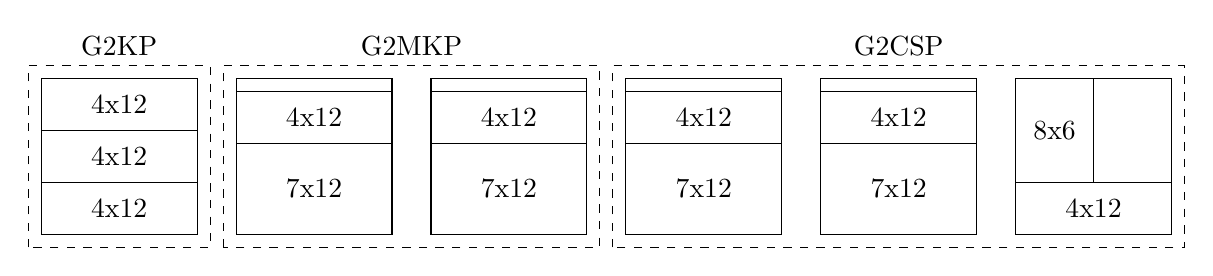
\begin{tikzpicture}[scale=0.165]
\def\piececolor{gray!20}
\def\labelxshift{12.5}
\def\labelyshift{0}
\def\labelfontsize{\normalsize}

\begin{scope}[shift={(0, 0)}]
\begin{scope}[shift={(0, 0)}]

\draw [dashed] (-1, -1) rectangle +(14, 14);
\path (-1, 13)  -- +(14, 0) node [above, midway, align=center] {\labelfontsize G2KP};

\draw (0, 0) rectangle +(12, 4) node[midway] {\labelfontsize 4x12};
\draw (0, 4) rectangle +(12, 4) node[midway] {\labelfontsize 4x12};
\draw (0, 8) rectangle +(12, 4) node[midway] {\labelfontsize 4x12};

\draw (0,0) rectangle +(12, 12);

\end{scope}

\begin{scope}[shift={(15, 0)}]

\draw [dashed] (-1, -1) rectangle +(29, 14);
\path (-1, 13) -- +(29, 0) node [above, midway, align=center] {\labelfontsize G2MKP};

\begin{scope}[shift={(0, 0)}]
\draw (0, 0) rectangle +(12, 7) node[midway] {\labelfontsize 7x12};
\draw (0, 7) rectangle +(12, 4) node[midway] {\labelfontsize 4x12};

\draw (0,0) rectangle +(12, 12);
\end{scope}

\begin{scope}[shift={(15, 0)}]
\draw (0, 0) rectangle +(12, 7) node[midway] {\labelfontsize 7x12};
\draw (0, 7) rectangle +(12, 4) node[midway] {\labelfontsize 4x12};

\draw (0,0) rectangle +(12, 12);
\end{scope}
\end{scope}
\end{scope}

\begin{scope}[shift={(45, 0)}]

\draw [dashed] (-1, -1) rectangle +(44, 14);
\path (-1, 13) -- +(44, 0) node [above, midway, align=center] {\labelfontsize G2CSP};

\begin{scope}[shift={(0, 0)}]
\draw (0, 0) rectangle +(12, 7) node[midway] {\labelfontsize 7x12};
\draw (0, 7) rectangle +(12, 4) node[midway] {\labelfontsize 4x12};

\draw (0,0) rectangle +(12, 12);
\end{scope}

\begin{scope}[shift={(15, 0)}]
\draw (0, 0) rectangle +(12, 7) node[midway] {\labelfontsize 7x12};
\draw (0, 7) rectangle +(12, 4) node[midway] {\labelfontsize 4x12};

\draw (0,0) rectangle +(12, 12);
\end{scope}

\begin{scope}[shift={(30, 0)}]
\draw (0, 0) rectangle +(12, 4) node[midway] {\labelfontsize 4x12};
\draw (0, 4) rectangle +(6, 8) node[midway] {\labelfontsize 8x6};

\draw (0,0) rectangle +(12, 12);

\end{scope}
\end{scope}


\end{tikzpicture}

  \vspace{3mm}
  \legend{The original plate dimensions and the piece multiset are the same for the three problems: \(L = W = 12\), \(l = [4, 7, 8]\), \(w = [12, 12, 6]\), \(u = [3, 2, 1]\), and profits equivalent to their respective areas. For G2MKP, \(m = 2\). G2CSP ignores the profits and consider \(u\) to be a lower bound. The only optimal solution for G2KP is a pattern that \emph{cannot} pertain to any optimal solution of either of the other two problems. Souce: the author.}
  \label{fig:related_problems_diagram}
\end{figure}

\emph{The original one-dimensional Bin Packing Problem (BPP)} and the one-dimensional CSP differ only in the expected diversity of the piece types in their respective instances. CSP instances typically have fewer piece types with a larger demand each, while BPP instances typically have more piece types with unitary (or very small) demand each.
Often a method that can solve the CSP can also solve the BPP and vice-versa, albeit it may be more effective at a specific level of piece type diversity.
The guillotine 2D variants of both problems are the same way, and, as such, the adapted formulation can solve both problems with low and high piece type diversity.
A priori, the BBA formulation does not favour one problem variant over the other.
The density of the cutting position discretization (and, therefore, size of the model) is not \emph{directly} correlated to piece type diversity; it has more to do with the number of pieces with small dimensions and how many linear combinations of the piece dimensions give the same value.
The G2CSP is also considered `a generalization of the 2D-BPP in which equivalent items are grouped into demands' (\url{http://or.dei.unibo.it/library/2dpacklib}).
If the definition above is adopted, then our method solves the G2CSP, as it groups identical pieces into a single piece type with a demand value.
For simplicity, the author chose to adopt G2CSP to refer to the problem to which the formulation was adapted.
However, the experiments include instances of piece diversity on both sides of the spectrum, examining the impact of piece type diversity.

\section{BBA formulation adaptations}
\label{sec:formulation_adaptation}

For the reader's convenience, the BBA formulation for the G2KP is replicated below\footnote{The formulation kept the same numbering from its original appearence.} accompanied by a refresher on how it works and its notation.
For the sake of consistency, the author chose to kept as much notation as possible. This means the input parameter~\(u\), which comes from \emph{u}pper bound, was kept in our adaptation of the formulation to G2OPP and G2CSP, even if in these problems it indicates a \emph{lower bound} instead.

%For the original model, reproduced by us in~\cref{sec:TODO}, \citet{furini:2016} already explains how to adapt the model to the G2SPP and G2CSP.
The sets we employ are the same as before and keep their usual meaning: \(\bar{J}\) -- the set of piece types, \(J \supseteq \bar{J}\) -- the set of all plate types, \(O = \{h, v\}\) -- the set of cut orientations (horizontal and vertical), \(Q_{jo}\) -- the sets of positions for which there is a cut of orientation~\(o\) over plate~\(j\) and, finally, \(E\) -- the set of piece extractions.
The following notation allow for easy access to pieces and plates related to the extractions: \(E_{i*} = \{ j : \exists~(i, j) \in E \}\) (which plates may have a copy of~\(i\) extracted from them) and \(E_{*j} = \{i : \exists~(i, j) \in E \}\) (which pieces may be extracted from a plate~\(j\)).

\begin{align*}
\bm{max.} &\sum_{(i, j) \in E} p_i e_{ij} \tag{\ref{eq:objfun}}\\
\bm{s.t.} &\specialcell{\sum_{o \in O}\sum_{q \in Q_{jo}} x^o_{qj} + \sum_{i \in E_{*j}} e_{ij} \leq \sum_{k \in J}\sum_{o \in O}\sum_{q \in Q_{ko}} a^o_{qkj} x^o_{qk} \hspace*{0.05\textwidth} \forall j \in J, j \neq 0,}\tag{\ref{eq:plates_conservation}}\\
%            & \specialcell{\sum_{o \in O}\sum_{q \in Q_{jo}} x^o_{qj} \leq \sum_{k \in J}\sum_{o \in O}\sum_{q \in Q_{ko}} a^o_{qkj} x^o_{qk} \hspace*{\fill} \forall j \in J\setminus\bar{J},}\label{eq:generic_plates_conservation}\\
	    & \specialcell{\sum_{o \in O}\sum_{q \in Q_{0o}} x^o_{q0} + \sum_{i \in E_{*0}} e_{i0} \leq 1 \hspace*{\fill},}\tag{\ref{eq:just_one_original_plate}}\\
            & \specialcell{\sum_{j \in E_{i*}} e_{ij} \leq u_i \hspace*{\fill} \forall i \in \bar{J},}\tag{\ref{eq:demand_limit}}\\
	    % TODO: fix equation below, the forall part is too long and clashes with the long equation in the first line
	    & \specialcell{x^o_{qj} \in \mathbb{N}^0 \hspace*{\fill} \forall j \in J, o \in O, q \in Q_{jo},}\tag{\ref{eq:trivial_x}}\\
            & \specialcell{e_{ij} \in \mathbb{N}^0 \hspace*{\fill} \forall (i, j) \in E.}\tag{\ref{eq:trivial_e}}
\end{align*}

The domain of all variables is the non-negative integers~\eqref{eq:trivial_x}-\eqref{eq:trivial_e}.
The value of a variable~\(e_{ij}\) indicates the number of times a piece~\(i\) was extracted from a  plate~\(j\).
An extraction only occurs if it respects the piece demand~\eqref{eq:demand_limit} (\(u_i\)~is the profit of piece~\(i\)) and, consequently, every extracted piece is taken into account by the objective function~\eqref{eq:objfun} which maximises the total profit (\(p_i\)~is the demand of piece~\(i\)).

The value of a variable~\(x^o_{qj}\) indicates the number of times (distinct instances of) a plate~\(j\) were cut at position \(q\) by a cut with orientation~\(o\).
Both~\eqref{eq:just_one_original_plate} and~\eqref{eq:plates_conservation} handle which plates are available and, therefore, may be further cut or have pieces extracted from them.
The only purpose of \eqref{eq:just_one_original_plate} is to make available one copy of the original plate (i.e., plate zero).
For each other plate type~\(j\), \eqref{eq:plates_conservation} guarantees that, for each copy of~\(j\) utilised for cutting or piece extraction, a copy of \(j\) was previously obtained from a larger plate.
The number of plate~\(j\) copies obtained by a cut at position~\(q\) and orientation~\(o\) over plate~\(k\) is given by~\(a^o_{qkj}\), this listing is a byproduct of the plate enumeration.

Each of the following inner sections considers a different problem.
For brevity, the adaptations do not replicate the changes necessary to allow piece rotation, but these changes are the same as the ones described for G2KP in~\cref{sec:adaptation_for_rotation}.

\subsection{Adaptation to Multiple Knapsack Problem}

To adapt the formulation for the G2KP to the (homogeneous) G2MKP, the only modification necessary is to replace the right-hand side of
\begin{flalign}
&& \sum_{o \in O}\sum_{q \in Q_{0o}} x^o_{q0} + \sum_{i \in E_{*0}} e_{i0} \leq 1 && \tag{\ref{eq:just_one_original_plate}}
\end{flalign}
with the number of available original plates.

\subsection{Adaptation to the homogeneous Cutting Stock Problem}

To adapt the formulation for the G2KP to the homogeneous G2CSP, it is enough to introduce a new integer variable~\(b\) and make the following changes to the formulation:

\begin{enumerate}
\item Replace the objective function~\eqref{eq:objfun} by \(\bm{min.}~b\).
\item Replace the literal~\(1\) in the right-hand side of~\eqref{eq:just_one_original_plate} by \(b\).
\item reverse the sense of the demand constraint, i.e., \cref{eq:demand_limit}, from \(\leq\) to \(\geq\).
\end{enumerate}

This formulation does not need an extra constraint to avoid the classic CSP symmetry problem in which the same number of used bins may be represented in multiple ways.
The formulation also does not need computing an upper bound on \(b\), i.e., the number of bins necessary, but it makes easy to provide one if available.

\subsection{Adaptation to the Orthogonal Packing Problem}

The employed adaptation of the formulation from the G2KP to the G2OPP consists only of two small changes.
The first change consists in reversing the sense of the demand constraint, i.e., \cref{eq:demand_limit}, from \(\leq\) to \(\geq\), as done in the adaptation for the G2CSP. %The sense could also be changed to equality, but solvers often have equivalent or better times if \(\leq\) or \(\geq\) is used instead of \(=\) when possible.
The second change consists in dropping the objective function.
If the model is feasible, then the solution to the decision problem is true; otherwise, it is false.

The adaptation for the G2OPP is not strictly necessary but an optimization.
The G2KP formulation could be directly applied to suitable G2OPP instances.
If absent, the piece type profit value may be set to be any positive value.
If the optimal solution for the G2KP is~\(\sum_{i\in\bar{J}} u_i p_i\), then the answer to the decision problem is true; otherwise, it is false.
The problem with this approach is that the solver may waste time maximizing the profit of the subset of packed pieces even when the upper bound already shows that it is impossible to pack every piece.
This problem may be solved by passing a cutoff parameter to the solver or adding an extra constraint to the formulation.
However, the author chose to change the demand constraint and drop the objective function for the experiments, as this adaptation better expresses the problem semantics to the solver.

\section{Chosen datasets and experiment results}

The author chose to use existing datasets from the literature when they were available and suitable to maximize the possibility of future direct or indirect comparisons.
For the G2OPP and the G2CSP, suitable datasets were selected from the literature.
The author did not find suitable datasets for the G2MKP in the literature and adapted previous instances from the literature to fill the gap.

\subsection{G2MKP}

The G2MKP is the least studied of the three problems discussed in this chapter.
As far as the author knows, the closest related work is~\citet{cui:2008} which proposes an exact algorithm for a special case of the three-staged G2MKP.
The special case \emph{disallow} the third stage to generate two or more piece types from the same intermediary plate.
The paper employs a subset of the FMT59 dataset adapted to have two or three original plates, i.e., \(m \in \{2, 3\}\), most of them solved in less than half a second.
The author of this thesis decided to not use these instances and, instead, adapted the A and CW datasets from the literature.
A is an unweighted real-world dataset with high-demand piece types from~\citet{macedo:2010} which is also employed in our G2CSP experiments.
CW is a weighted artificial dataset with low-demand piece types from~\citet{fayard:1998} which is also employed in our G2KP experiments.
The adopted criteria for allowing an instance to have \(m \in \{2, 4, 8\}\) is that the summed area of the original plates is at most half the summed piece area.
This way, the \emph{selection} aspect of the problem is retained.

\begin{table}[!t]
\centering
\caption{Results for CW\_M dataset (G2MKP) with and without rotation.}
\label{tab:G2MKP_CW_joined}
\begin{tabular}{lrrrrrr}
\hline\hline\
& \multicolumn{3}{c}{No Rotation} & \multicolumn{3}{c}{R. \& Mirror Plates} \\\cmidrule(lr){2-4}\cmidrule(lr){5-7}
Inst. & BKV & \#nz & T. (s) & BKV & \#nz & T. (s) \\\hline
CW01\_M2 & 12085 & 54,403 & 4.68 & 12227 & 150,308 & 254.11 \\
\rowcolor{gray-inner-row} CW01\_M4 & 20093 & \ditto & >3600 & 20422 & \ditto & >3600 \\
CW02\_M2 & 10519 & 56,140 & 2.11 & 10943 & 143,098 & 16.81 \\
\rowcolor{gray-inner-row} CW02\_M4 & 17384 & \ditto & >3600 & 17680 & \ditto & >3600 \\
CW03\_M2 & 10648 & 121,581 & 3.75 & 10877 & 491,790 & 69.33 \\
\rowcolor{gray-inner-row} CW03\_M4 & 19113 & \ditto & 10.38 & 19577 & \ditto & 25.77 \\
CW04\_M2 & 11591 & 71,221 & 0.61 & 12412 & 497,740 & 23.66 \\
\rowcolor{gray-inner-row} CW04\_M4 & 18104 & \ditto & 57.29 & 19443 & \ditto & >3600 \\
CW05\_M2 & 21469 & 93,269 & 0.86 & 21657 & 700,304 & 835.05 \\
\rowcolor{gray-inner-row} CW05\_M4 & 34358 & \ditto & 43.38 & 35199 & \ditto & 48.27 \\
CW06\_M2 & 23379 & 525,199 & >3600 & 23639 & 2,872,208 & >3600 \\
\rowcolor{gray-inner-row} CW06\_M4 & 35407 & \ditto & >3600 & 35803 & \ditto & >3600 \\
\rowcolor{gray-table-row} CW06\_M8 & 52046 & \ditto & >3600 & 52674 & \ditto & >3600 \\
CW07\_M2 & 18834 & 123,851 & 3.28 & 19755 & 784,086 & 73.13 \\
\rowcolor{gray-inner-row} CW07\_M4 & 33519 & \ditto & >3600 & 35007 & \ditto & >3600 \\
\rowcolor{gray-table-row} CW07\_M8 & 53631 & \ditto & >3600 & 54835 & \ditto & >3600 \\
CW08\_M2 & 8923 & 408,428 & 10.33 & 8985 & 1,174,315 & >3600 \\
\rowcolor{gray-inner-row} CW08\_M4 & 15074 & \ditto & 684.15 & 15448 & \ditto & >3600 \\
\rowcolor{gray-table-row} CW08\_M8 & 24909 & \ditto & >3600 & 25241 & \ditto & >3600 \\
CW09\_M2 & 18712 & 204,212 & 1,525.83 & 19758 & 917,729 & 207.43 \\
\rowcolor{gray-inner-row} CW09\_M4 & 30182 & \ditto & 171.65 & 31174 & \ditto & >3600 \\
\rowcolor{gray-table-row} CW09\_M8 & 46695 & \ditto & >3600 & 47259 & \ditto & >3600 \\
CW10\_M2 & 12441 & 383,575 & 8.37 & 13047 & 2,714,389 & 98.02 \\
\rowcolor{gray-inner-row} CW10\_M4 & 23065 & \ditto & >3600 & 24088 & \ditto & >3600 \\
\rowcolor{gray-table-row} CW10\_M8 & 37827 & \ditto & >3600 & 38655 & \ditto & >3600 \\
CW11\_M2 & 12078 & 384,237 & 7.16 & 12437 & 2,710,188 & 621.13 \\
\rowcolor{gray-inner-row} CW11\_M4 & 22752 & \ditto & 286.38 & 23419 & \ditto & >3600 \\
\rowcolor{gray-table-row} CW11\_M8 & 36691 & \ditto & 96.72 & 37191 & \ditto & >3600 \\\hline\hline
\end{tabular}
\legend{The best known value (BKV) is optimal if the run did not finish because timeout (indicated by \emph{>3600}). \emph{\#nz} stands for number of nonzeros (which is always the same for instances adapted from the same original instance). The background color of the rows indicates the number of original plates.}
\end{table}

Generally, for the adapted CW dataset, increasing the number of original plates available increases the time to solve, and allowing rotation (with the mirror plate enhancement) has a similar effect.
These effects can be seen in~\cref{tab:G2MKP_CW_joined}.
Increasing the number of original plates changes only a single right-hand side value, but allowing rotation causes a considerable increase in the model size, ranging from the \(\approx 2.8\) times of CW08\_* to the \(\approx 7.5\) times of CW05\_*.
Both changes increase the search space, but this does not always translate directly to a larger gap between lower and upper bounds or a larger number of nodes needed to close it.
In most cases, the time spent in the root node relaxation is relatively small, especially in the runs that end in timeout, as it can be seen in~\cref{fig:g2mkp_cw_histogram_barrier_percent_time}.

\begin{figure}[!htbp]
  \caption{Impact of solving the root node in CW\_M dataset (G2MKP).}
  \center
  \includegraphics[width=0.8\linewidth]{plots/g2mkp_cw_histogram_barrier_percent_time.pdf}
  \legend{Souce: the author.}
  \label{fig:g2mkp_cw_histogram_barrier_percent_time}
\end{figure}

The time increase caused by rotation has a single exception, CW09\_M2.
For CW09\_M2, the barrier times with and without rotation are, respectively, 45 and 3 seconds; the optimal solution, with and without rotation, are found, respectively, at 61 seconds (1.21\% of gap) and 6 seconds (0.36\% of gap); despite that, in 3864 nodes (206 seconds) the run allowing rotation closes the gap, while the run without rotation takes 317502 nodes (1525 seconds) to do the same.
So, there is no other factor at play for this particular instance except the branching needing fewer nodes to tighten the upper bound enough to close the gap.

% ROTATION CW03_M2 10s root 21s best 1.56 gap 0 node no relax change at the moment
% ROTATION CW03_M4  9s root 22s best 0.35 gap 0 node no relax change at the moment
% ROTATION CW05_M2 17s root 27s best 2.66 gap 0 node no relax change at the moment 830 total
% ROTATION CW05_M4 14s root 43s best 0.23 gap 0 node no relax change at the moment45s total
% CW09_M2 3s root  6s best 0.36 gap   0 node 1525s total
% CW09_M4 2s root 15s best 0.33 gap 172 node  171s total
% CW11_M4 3s root 14s best 0.58 gap   0 node  285s total
% CW11_M8 3s root 49s best 0.22 gap   0 node   95s total

% CW11_M2 3s root  5s best 0.26 gap   0 node    5s total
%CW08_M{2,4} (no rotation), 
% CW08_M2 9s root 9s best 0.00 gap 0 node, instance close
% CW08_M4 9s root 21s best 0.53 gap 0 node no relax change at the moment TOTAL 680s
% CW01_M2 0.5s root 2s best 1.81 gap 0 node no relax change at the moment (4s total)
% UNFINISHED CW01_M4 0.5s root 134s best 1.59 gap 1045 node (relax change)

The other set of exceptions (related to the change of~\(m\)) has a behaviour similar to the case reported above.
These exceptions are CW03\_M{2,4} (rotation), CW05\_M{2,4} (rotation), CW09\_M{2,4} (no rotation), and CW11\_M{4,8} (no rotation).
In these cases, the time spent solving the root node is similar (respectively, 10s vs 9s, 17s vs 14s, 3s vs 2s, and 3s vs 3s), the larger \(m\) takes the same or more time to find the optimal solution (respectively, 21s vs 22s, 27s vs 43s, 6s vs 15s, and 14s vs 49s).
However, the percentage gap when the solver finds the optimal solution is either similar or lower (1.56 vs 0.35, 2.66 vs 0.23, 0.36 vs 0.33, and 0.58 vs 0.22 gap), which seems to result in lower total times (69s vs 26s, 830s vs 45s, 1525s vs 171s, 285s vs 95s).
In most cases, the solver finds the optimal solution before starting branching (by employing heuristics).
Therefore, the reported gap is against the root node relaxation (solved with any extra cuts added by the solver).

Considering only the instances for which both runs obtained an optimal solution (11 of the 28), the profit gap between optimal solution allowing and not allowing rotation ranges between 0.87\% and 7.08\% increase.

A final observation about the CW dataset is that CW10 and CW11 are very similar. They just have slightly different original plate dimensions (respectively, 992x970 vs 982x967), and their piece types have the same \(l\), \(w\), and \(p\), i.e., just the demand~\(u\) has different values. However, the timings of CW10 and CW11 are considerably distinct, showing how much depends on the specific values of an instance.

\begin{table}[!htbp]
\centering
\caption{Results for A\_M dataset (G2MKP) with and without rotation.}
\label{tab:G2MKP_A_joined}
\resizebox{!}{0.95\height}{%
\begin{tabular}{lrrrrrr}
\hline\hline
& \multicolumn{3}{c}{No Rotation} & \multicolumn{3}{c}{R. \& Mirror Plates} \\\cmidrule(lr){2-4}\cmidrule(lr){5-7}
Inst. & BKV & \#nz & T. (s) & BKV & \#nz & T. (s) \\\hline
A03\_M2 & 4,201,018 & 27 & 0.00 & 4,201,018 & 60 & 0.02 \\
A17\_M2 & 10,336,720 & 10,123 & 0.29 & 10,639,320 & 223,328 & 9.80 \\
A26\_M2 & 0 & 9,692,187 & >3600 & -- & -- & OOM \\
A31\_M2 & 0 & 4,184,736 & >3600 & -- & 89,405,895 & OOM \\
A34\_M2 & 10,350,034 & 390,377 & 138.87 & 0 & 10,434,707 & >3600 \\
A36\_M2 & 10,078,104 & 273,536 & 50.65 & 0 & 6,914,749 & >3600 \\
A37\_M2 & 10,368,156 & 31,225 & 0.76 & 10,535,478 & 1,027,417 & 201.73 \\
A42\_M2 & 5,060,407 & 155 & 0.03 & 5,954,727 & 981 & 0.30 \\
A43\_M2 & 5,837,348 & 9,244 & 0.12 & 6,293,486 & 207,767 & 8.14 \\
A05\_M2 & 10,134,040 & 104,146 & 2.66 & 10,199,480 & 2,289,561 & 1,268.31 \\
\rowcolor{gray-inner-row} A05\_M4 & 19,967,032 & \ditto & 2.93 & 20,373,040 & \ditto & 1,392.24 \\
A07\_M2 & 5,759,424 & 428 & 0.02 & 6,338,432 & 5,247 & 0.05 \\
\rowcolor{gray-inner-row} A07\_M4 & 10,992,036 & \ditto & 0.02 & 12,518,720 & \ditto & 0.04 \\
A12\_M2 & 9,238,568 & 89 & 0.66 & 9,925,676 & 337 & 0.30 \\
\rowcolor{gray-inner-row} A12\_M4 & 18,472,968 & \ditto & 0.01 & 19,847,184 & \ditto & 0.31 \\
A13\_M2 & 10,595,594 & 1,773,362 & 496.74 & -- & -- & OOM \\
\rowcolor{gray-inner-row} A13\_M4 & 21,010,004 & \ditto & 492.58 & -- & \ditto & OOM \\
A23\_M2 & 10,492,334 & 155,995 & 6.12 & 0 & 5,209,384 & >3600 \\
\rowcolor{gray-inner-row} A23\_M4 & 20,975,576 & \ditto & 6.44 & 0 & \ditto & >3600 \\
A40\_M2 & 6,645,196 & 315,554 & 37.00 & 6,656,196 & 3,981,752 & 2,209.75 \\
\rowcolor{gray-inner-row} A40\_M4 & 13,252,696 & \ditto & 41.63 & 13,277,288 & \ditto & >3600 \\
A41\_M2 & 6,576,896 & 1,244,457 & 193.32 & -- & 31,283,337 & OOM \\
\rowcolor{gray-inner-row} A41\_M4 & 13,061,346 & \ditto & 163.99 & -- & \ditto & OOM \\
A02\_M2 & 4,671,806 & 81 & 0.28 & 4,671,806 & 666 & 0.04 \\
\rowcolor{gray-inner-row} A02\_M4 & 9,079,396 & \ditto & 0.01 & 9,079,396 & \ditto & 0.02 \\
\rowcolor{gray-table-row} A02\_M8 & 17,894,576 & \ditto & 0.01 & 17,894,576 & \ditto & 0.02 \\
A15\_M2 & 10,431,108 & 84,144 & 1.31 & 10,591,164 & 1,905,324 & 241.80 \\
\rowcolor{gray-inner-row} A15\_M4 & 20,821,776 & \ditto & 1.16 & 21,112,992 & \ditto & 245.26 \\
\rowcolor{gray-table-row} A15\_M8 & 41,359,738 & \ditto & 2.44 & 42,058,060 & \ditto & 291.12 \\
A20\_M2 & 10,481,602 & 499,945 & 42.26 & -- & 32,487,621 & OOM \\
\rowcolor{gray-inner-row} A20\_M4 & 20,888,454 & \ditto & 46.32 & -- & \ditto & OOM \\
\rowcolor{gray-table-row} A20\_M8 & 41,474,893 & \ditto & >3600 & -- & \ditto & OOM \\
A21\_M2 & 10,607,622 & 5,937,528 & 3,512.46 & -- & -- & OOM \\
\rowcolor{gray-inner-row} A21\_M4 & 0 & \ditto & >3600 & -- & \ditto & OOM \\
\rowcolor{gray-table-row} A21\_M8 & 0 & \ditto & >3600 & -- & \ditto & OOM \\
\hline\hline
\end{tabular} } % resizebox
\vspace{1mm}
\legend{Similar to \cref{tab:G2MKP_CW_joined}. OOM means \emph{out of memory}. The instances are grouped by number of adaptations, i.e., first the instances that only have \(m = 2\), then the ones with \(m \in \{2, 4\}\), and finally the ones with \(m \in \{2, 4, 8\}\). Inside each group the instances are sorted by name. Source: the author.}
\end{table}

The author chose to exclude from~\cref{tab:G2MKP_A_joined} every instance for which both runs (with and without rotation) did not obtain a solution or obtained the trivial (i.e., empty) solution.
Most of these runs failed due to memory exhaustion and did not even provide the number of nonzeros (i.e., failed before Gurobi loaded the model).
Except by A21\_M2, if an adapted instance was excluded for the reason above, then all the adapted instances sharing the same original instance (i.e., sharing the name before the underline) were also excluded for the same reason.
This detail indicates that, in general, what determined if an instance was hard to solve were the other instance characteristics besides the~\(m\).
The full list of adapted instances can be found in~\cref{sec:datasets} (under item \emph{A-*\_M2, A-*\_M4, A-\_M8}).

The A\_M dataset behaves differently from the previous CW\_M dataset.
In the A\_M runs, increasing \(m\) often has little effect on the solving times.
Also, the time spent solving the root node is more significant, as shown in~\cref{fig:g2mkp_cw_histogram_barrier_percent_time}.
A more detailed examination of A13\_M{2,4} (no rotation) shows that almost all time is spent solving the root node (respectively, 457s and 419s); the optimal solutions are found shortly after (respectively, by the 484s and the 479s) with a very small gap (0.03\% and 0.06\%) which is soon closed.

\begin{figure}[!t]
  \caption{Impact of solving the root node in A\_M dataset (G2MKP).\\(Only runs that did not suffer memory exhaustion.)}
  \center
  \includegraphics[width=0.8\linewidth]{plots/g2mkp_a_histogram_barrier_percent_time.pdf}
  \legend{Souce: the author.}
  \label{fig:g2mkp_a_histogram_barrier_percent_time}
\end{figure}

One explanation for the similar timings, is that, given the instances are unweighted and have a high piece demand, the problem with \(m = 2\) is not very distinct from the problem with \(m = 4\).
The optimal solutions found for A13\_M{2,4} corroborate this explanation: the original instance had \(u = [10, 12, 120, 40, 80, 10, 8, 24]\), and the solutions for the \(m \in \{2, 4\}\) instances employ the following numbers of pieces, respectively, \([0, 0, 16, 18, 16, 4, 8, 18]\) and \([0, 0, 34, 34, 40, 10, 8, 24]\), i.e., the demand for the last two piece types are the only ones low enough impede the \(m = 4\) solutions to be just a repetition of the same pattern used in both plates of the \(m = 2\) optimal solution. For reference, the patterns present in both solutions are presented in~\cref{fig:g2mkp_a14_24}.

\begin{figure}[!t]
  \caption{Cutting patterns present in optimal solutions of A13\_M\{2,4\} (G2MKP).}
  \center
  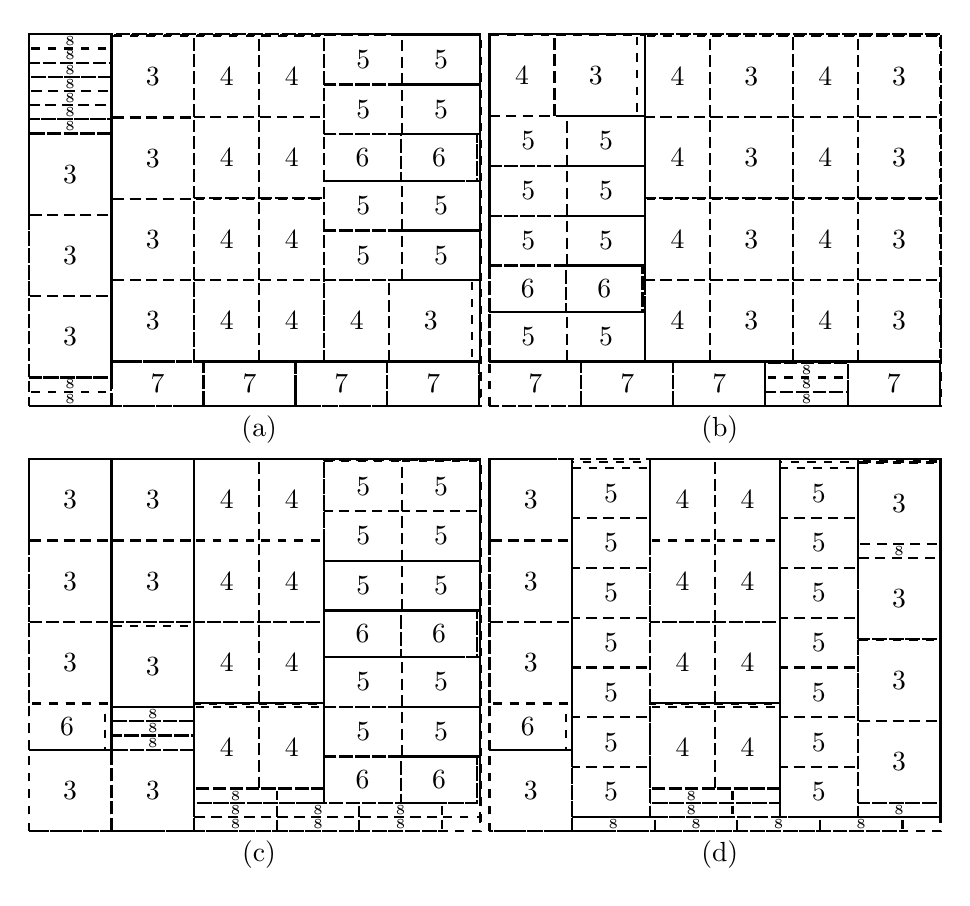
\begin{tikzpicture}[scale=0.225]
\def\labelfontsize{\normalsize}
\def\labelfontsizeeight{\tiny}
\def\firstpattern {
\draw[dashed, thick, black] (0.0, 0.0) rectangle (4.66, 0.8);
\node[font=\labelfontsizeeight] at (2.33, 0.4) {8};
%\node[font=\labelfontsize] at (2.33, 0.4) {466x80};
\draw[dashed, thick, black] (0.0, 0.8) rectangle (4.66, 1.6);
\node[font=\labelfontsizeeight] at (2.33, 1.2) {8};
%\node[font=\labelfontsize] at (2.33, 1.2) {466x80};
\draw[dashed, thick, black] (0.0, 0.0) rectangle (4.66, 1.6);
\draw[dashed, thick, black] (0.0, 1.6) rectangle (4.67, 6.19);
\node[font=\labelfontsize] at (2.335, 3.895) {3};
%\node[font=\labelfontsize] at (2.335, 3.895) {467x459};
\draw[dashed, thick, black] (0.0, 6.19) rectangle (4.67, 10.78);
\node[font=\labelfontsize] at (2.335, 8.485) {3};
%\node[font=\labelfontsize] at (2.335, 8.485) {467x459};
\draw[dashed, thick, black] (0.0, 10.78) rectangle (4.67, 15.37);
\node[font=\labelfontsize] at (2.335, 13.075) {3};
%\node[font=\labelfontsize] at (2.335, 13.075) {467x459};
\draw[dashed, thick, black] (0.0, 15.37) rectangle (4.66, 16.17);
\node[font=\labelfontsizeeight] at (2.33, 15.77) {8};
%\node[font=\labelfontsize] at (2.33, 15.77) {466x80};
\draw[dashed, thick, black] (0.0, 16.17) rectangle (4.66, 16.97);
\node[font=\labelfontsizeeight] at (2.33, 16.57) {8};
%\node[font=\labelfontsize] at (2.33, 16.57) {466x80};
\draw[dashed, thick, black] (0.0, 16.97) rectangle (4.66, 17.77);
\node[font=\labelfontsizeeight] at (2.33, 17.37) {8};
%\node[font=\labelfontsize] at (2.33, 17.37) {466x80};
\draw[dashed, thick, black] (0.0, 17.77) rectangle (4.66, 18.57);
\node[font=\labelfontsizeeight] at (2.33, 18.17) {8};
%\node[font=\labelfontsize] at (2.33, 18.17) {466x80};
\draw[dashed, thick, black] (0.0, 18.57) rectangle (4.66, 19.37);
\node[font=\labelfontsizeeight] at (2.33, 18.97) {8};
%\node[font=\labelfontsize] at (2.33, 18.97) {466x80};
\draw[dashed, thick, black] (0.0, 19.37) rectangle (4.66, 20.17);
\node[font=\labelfontsizeeight] at (2.33, 19.77) {8};
%\node[font=\labelfontsize] at (2.33, 19.77) {466x80};
\draw[dashed, thick, black] (0.0, 20.17) rectangle (4.66, 20.97);
\node[font=\labelfontsizeeight] at (2.33, 20.57) {8};
%\node[font=\labelfontsize] at (2.33, 20.57) {466x80};
\draw[dashed, thick, black] (0.0, 19.37) rectangle (4.66, 20.97);
\draw[dashed, thick, black] (0.0, 18.57) rectangle (4.66, 20.97);
\draw[dashed, thick, black] (0.0, 17.77) rectangle (4.66, 20.97);
\draw[dashed, thick, black] (0.0, 16.97) rectangle (4.66, 20.97);
\draw[dashed, thick, black] (0.0, 16.17) rectangle (4.67, 20.97);
\draw[dashed, thick, black] (0.0, 15.37) rectangle (4.67, 20.99);
\draw[dashed, thick, black] (0.0, 10.78) rectangle (4.67, 21.0);
\draw[dashed, thick, black] (0.0, 6.19) rectangle (4.67, 21.0);
\draw[dashed, thick, black] (0.0, 1.6) rectangle (4.67, 21.0);
\draw[dashed, thick, black] (0.0, 0.0) rectangle (4.67, 21.0);
\draw[dashed, thick, black] (4.67, 0.0) rectangle (9.86, 2.5);
\node[font=\labelfontsize] at (7.265, 1.25) {7};
%\node[font=\labelfontsize] at (7.265, 1.25) {519x250};
\draw[dashed, thick, black] (9.86, 0.0) rectangle (15.05, 2.5);
\node[font=\labelfontsize] at (12.455, 1.25) {7};
%\node[font=\labelfontsize] at (12.455, 1.25) {519x250};
\draw[dashed, thick, black] (4.67, 0.0) rectangle (15.05, 2.5);
\draw[dashed, thick, black] (15.05, 0.0) rectangle (20.24, 2.5);
\node[font=\labelfontsize] at (17.645, 1.25) {7};
%\node[font=\labelfontsize] at (17.645, 1.25) {519x250};
\draw[dashed, thick, black] (20.24, 0.0) rectangle (25.43, 2.5);
\node[font=\labelfontsize] at (22.835, 1.25) {7};
%\node[font=\labelfontsize] at (22.835, 1.25) {519x250};
\draw[dashed, thick, black] (15.05, 0.0) rectangle (25.43, 2.5);
\draw[dashed, thick, black] (4.67, 0.0) rectangle (25.43, 2.5);
\draw[dashed, thick, black] (4.67, 2.5) rectangle (9.34, 7.09);
\node[font=\labelfontsize] at (7.005, 4.795) {3};
%\node[font=\labelfontsize] at (7.005, 4.795) {467x459};
\draw[dashed, thick, black] (4.67, 7.09) rectangle (9.34, 11.68);
\node[font=\labelfontsize] at (7.005, 9.385) {3};
%\node[font=\labelfontsize] at (7.005, 9.385) {467x459};
\draw[dashed, thick, black] (4.67, 2.5) rectangle (9.34, 11.68);
\draw[dashed, thick, black] (4.67, 11.68) rectangle (9.34, 16.27);
\node[font=\labelfontsize] at (7.005, 13.975) {3};
%\node[font=\labelfontsize] at (7.005, 13.975) {467x459};
\draw[dashed, thick, black] (4.67, 16.27) rectangle (9.34, 20.86);
\node[font=\labelfontsize] at (7.005, 18.565) {3};
%\node[font=\labelfontsize] at (7.005, 18.565) {467x459};
\draw[dashed, thick, black] (4.67, 11.68) rectangle (9.34, 20.91);
\draw[dashed, thick, black] (4.67, 2.5) rectangle (9.34, 20.97);
\draw[dashed, thick, black] (9.34, 2.5) rectangle (13.01, 7.09);
\node[font=\labelfontsize] at (11.175, 4.795) {4};
%\node[font=\labelfontsize] at (11.175, 4.795) {367x459};
\draw[dashed, thick, black] (13.01, 2.5) rectangle (16.68, 7.09);
\node[font=\labelfontsize] at (14.845, 4.795) {4};
%\node[font=\labelfontsize] at (14.845, 4.795) {367x459};
\draw[dashed, thick, black] (9.34, 2.5) rectangle (16.68, 7.09);
\draw[dashed, thick, black] (9.34, 7.09) rectangle (13.01, 11.68);
\node[font=\labelfontsize] at (11.175, 9.385) {4};
%\node[font=\labelfontsize] at (11.175, 9.385) {367x459};
\draw[dashed, thick, black] (13.01, 7.09) rectangle (16.68, 11.68);
\node[font=\labelfontsize] at (14.845, 9.385) {4};
%\node[font=\labelfontsize] at (14.845, 9.385) {367x459};
\draw[dashed, thick, black] (9.34, 7.09) rectangle (16.68, 11.68);
\draw[dashed, thick, black] (9.34, 2.5) rectangle (16.68, 11.71);
\draw[dashed, thick, black] (9.34, 11.71) rectangle (13.01, 16.3);
\node[font=\labelfontsize] at (11.175, 14.005) {4};
%\node[font=\labelfontsize] at (11.175, 14.005) {367x459};
\draw[dashed, thick, black] (13.01, 11.71) rectangle (16.68, 16.3);
\node[font=\labelfontsize] at (14.845, 14.005) {4};
%\node[font=\labelfontsize] at (14.845, 14.005) {367x459};
\draw[dashed, thick, black] (9.34, 11.71) rectangle (16.68, 16.3);
\draw[dashed, thick, black] (9.34, 16.3) rectangle (13.01, 20.89);
\node[font=\labelfontsize] at (11.175, 18.595) {4};
%\node[font=\labelfontsize] at (11.175, 18.595) {367x459};
\draw[dashed, thick, black] (13.01, 16.3) rectangle (16.68, 20.89);
\node[font=\labelfontsize] at (14.845, 18.595) {4};
%\node[font=\labelfontsize] at (14.845, 18.595) {367x459};
\draw[dashed, thick, black] (9.34, 16.3) rectangle (16.68, 20.89);
\draw[dashed, thick, black] (9.34, 11.71) rectangle (16.68, 20.94);
\draw[dashed, thick, black] (9.34, 2.5) rectangle (16.68, 21.0);
\draw[dashed, thick, black] (16.68, 2.5) rectangle (20.35, 7.09);
\node[font=\labelfontsize] at (18.515, 4.795) {4};
%\node[font=\labelfontsize] at (18.515, 4.795) {367x459};
\draw[dashed, thick, black] (20.35, 2.5) rectangle (25.02, 7.09);
\node[font=\labelfontsize] at (22.685, 4.795) {3};
%\node[font=\labelfontsize] at (22.685, 4.795) {467x459};
\draw[dashed, thick, black] (16.68, 2.5) rectangle (25.46, 7.09);
\draw[dashed, thick, black] (16.68, 7.09) rectangle (21.07, 9.9);
\node[font=\labelfontsize] at (18.875, 8.495) {5};
%\node[font=\labelfontsize] at (18.875, 8.495) {439x281};
\draw[dashed, thick, black] (21.07, 7.09) rectangle (25.46, 9.9);
\node[font=\labelfontsize] at (23.265, 8.495) {5};
%\node[font=\labelfontsize] at (23.265, 8.495) {439x281};
\draw[dashed, thick, black] (16.68, 7.09) rectangle (25.46, 9.9);
\draw[dashed, thick, black] (16.68, 9.9) rectangle (21.07, 12.71);
\node[font=\labelfontsize] at (18.875, 11.305) {5};
%\node[font=\labelfontsize] at (18.875, 11.305) {439x281};
\draw[dashed, thick, black] (21.07, 9.9) rectangle (25.46, 12.71);
\node[font=\labelfontsize] at (23.265, 11.305) {5};
%\node[font=\labelfontsize] at (23.265, 11.305) {439x281};
\draw[dashed, thick, black] (16.68, 9.9) rectangle (25.46, 12.71);
\draw[dashed, thick, black] (16.68, 7.09) rectangle (25.46, 12.71);
\draw[dashed, thick, black] (16.68, 12.71) rectangle (21.0, 15.32);
\node[font=\labelfontsize] at (18.84, 14.015) {6};
%\node[font=\labelfontsize] at (18.84, 14.015) {432x261};
\draw[dashed, thick, black] (21.0, 12.71) rectangle (25.32, 15.32);
\node[font=\labelfontsize] at (23.16, 14.015) {6};
%\node[font=\labelfontsize] at (23.16, 14.015) {432x261};
\draw[dashed, thick, black] (16.68, 12.71) rectangle (25.32, 15.32);
\draw[dashed, thick, black] (16.68, 15.32) rectangle (21.07, 18.13);
\node[font=\labelfontsize] at (18.875, 16.725) {5};
%\node[font=\labelfontsize] at (18.875, 16.725) {439x281};
\draw[dashed, thick, black] (21.07, 15.32) rectangle (25.46, 18.13);
\node[font=\labelfontsize] at (23.265, 16.725) {5};
%\node[font=\labelfontsize] at (23.265, 16.725) {439x281};
\draw[dashed, thick, black] (16.68, 15.32) rectangle (25.46, 18.13);
\draw[dashed, thick, black] (16.68, 18.13) rectangle (21.07, 20.94);
\node[font=\labelfontsize] at (18.875, 19.535) {5};
%\node[font=\labelfontsize] at (18.875, 19.535) {439x281};
\draw[dashed, thick, black] (21.07, 18.13) rectangle (25.46, 20.94);
\node[font=\labelfontsize] at (23.265, 19.535) {5};
%\node[font=\labelfontsize] at (23.265, 19.535) {439x281};
\draw[dashed, thick, black] (16.68, 18.13) rectangle (25.46, 20.94);
\draw[dashed, thick, black] (16.68, 15.32) rectangle (25.46, 20.94);
\draw[dashed, thick, black] (16.68, 12.71) rectangle (25.46, 20.94);
\draw[dashed, thick, black] (16.68, 7.09) rectangle (25.46, 21.0);
\draw[dashed, thick, black] (16.68, 2.5) rectangle (25.46, 21.0);
\draw[dashed, thick, black] (9.34, 2.5) rectangle (25.46, 21.0);
\draw[dashed, thick, black] (4.67, 2.5) rectangle (25.46, 21.0);
\draw[dashed, thick, black] (4.67, 0.0) rectangle (25.46, 21.0);
\draw[dashed, thick, black] (0.0, 0.0) rectangle (25.5, 21.0);
}
\def\secondpattern {
\draw[dashed, thick, black] (0.0, 0.0) rectangle (5.19, 2.5);
\node[font=\labelfontsize] at (2.595, 1.25) {7};
%\node[font=\labelfontsize] at (2.595, 1.25) {519x250};
\draw[dashed, thick, black] (5.19, 0.0) rectangle (10.38, 2.5);
\node[font=\labelfontsize] at (7.785, 1.25) {7};
%\node[font=\labelfontsize] at (7.785, 1.25) {519x250};
\draw[dashed, thick, black] (10.38, 0.0) rectangle (15.57, 2.5);
\node[font=\labelfontsize] at (12.975, 1.25) {7};
%\node[font=\labelfontsize] at (12.975, 1.25) {519x250};
\draw[dashed, thick, black] (15.57, 0.0) rectangle (20.23, 0.8);
\node[font=\labelfontsizeeight] at (17.9, 0.4) {8};
%\node[font=\labelfontsize] at (17.9, 0.4) {466x80};
\draw[dashed, thick, black] (15.57, 0.8) rectangle (20.23, 1.6);
\node[font=\labelfontsizeeight] at (17.9, 1.2) {8};
%\node[font=\labelfontsize] at (17.9, 1.2) {466x80};
\draw[dashed, thick, black] (15.57, 1.6) rectangle (20.23, 2.4);
\node[font=\labelfontsizeeight] at (17.9, 2.0) {8};
%\node[font=\labelfontsize] at (17.9, 2.0) {466x80};
\draw[dashed, thick, black] (15.57, 0.8) rectangle (20.23, 2.4);
\draw[dashed, thick, black] (15.57, 0.0) rectangle (20.23, 2.4);
\draw[dashed, thick, black] (20.23, 0.0) rectangle (25.42, 2.5);
\node[font=\labelfontsize] at (22.825, 1.25) {7};
%\node[font=\labelfontsize] at (22.825, 1.25) {519x250};
\draw[dashed, thick, black] (15.57, 0.0) rectangle (25.42, 2.5);
\draw[dashed, thick, black] (10.38, 0.0) rectangle (25.42, 2.5);
\draw[dashed, thick, black] (5.19, 0.0) rectangle (25.42, 2.5);
\draw[dashed, thick, black] (0.0, 0.0) rectangle (25.42, 2.5);
\draw[dashed, thick, black] (0.0, 2.5) rectangle (4.39, 5.31);
\node[font=\labelfontsize] at (2.195, 3.905) {5};
%\node[font=\labelfontsize] at (2.195, 3.905) {439x281};
\draw[dashed, thick, black] (4.39, 2.5) rectangle (8.78, 5.31);
\node[font=\labelfontsize] at (6.585, 3.905) {5};
%\node[font=\labelfontsize] at (6.585, 3.905) {439x281};
\draw[dashed, thick, black] (0.0, 2.5) rectangle (8.78, 5.31);
\draw[dashed, thick, black] (0.0, 5.31) rectangle (4.32, 7.92);
\node[font=\labelfontsize] at (2.16, 6.615) {6};
%\node[font=\labelfontsize] at (2.16, 6.615) {432x261};
\draw[dashed, thick, black] (4.32, 5.31) rectangle (8.64, 7.92);
\node[font=\labelfontsize] at (6.48, 6.615) {6};
%\node[font=\labelfontsize] at (6.48, 6.615) {432x261};
\draw[dashed, thick, black] (0.0, 5.31) rectangle (8.64, 7.92);
\draw[dashed, thick, black] (0.0, 7.92) rectangle (4.39, 10.73);
\node[font=\labelfontsize] at (2.195, 9.325) {5};
%\node[font=\labelfontsize] at (2.195, 9.325) {439x281};
\draw[dashed, thick, black] (4.39, 7.92) rectangle (8.78, 10.73);
\node[font=\labelfontsize] at (6.585, 9.325) {5};
%\node[font=\labelfontsize] at (6.585, 9.325) {439x281};
\draw[dashed, thick, black] (0.0, 7.92) rectangle (8.78, 10.73);
\draw[dashed, thick, black] (0.0, 5.31) rectangle (8.78, 10.73);
\draw[dashed, thick, black] (0.0, 2.5) rectangle (8.78, 10.73);
\draw[dashed, thick, black] (0.0, 10.73) rectangle (4.39, 13.54);
\node[font=\labelfontsize] at (2.195, 12.135) {5};
%\node[font=\labelfontsize] at (2.195, 12.135) {439x281};
\draw[dashed, thick, black] (4.39, 10.73) rectangle (8.78, 13.54);
\node[font=\labelfontsize] at (6.585, 12.135) {5};
%\node[font=\labelfontsize] at (6.585, 12.135) {439x281};
\draw[dashed, thick, black] (0.0, 10.73) rectangle (8.78, 13.54);
\draw[dashed, thick, black] (0.0, 13.54) rectangle (4.39, 16.35);
\node[font=\labelfontsize] at (2.195, 14.945) {5};
%\node[font=\labelfontsize] at (2.195, 14.945) {439x281};
\draw[dashed, thick, black] (4.39, 13.54) rectangle (8.78, 16.35);
\node[font=\labelfontsize] at (6.585, 14.945) {5};
%\node[font=\labelfontsize] at (6.585, 14.945) {439x281};
\draw[dashed, thick, black] (0.0, 13.54) rectangle (8.78, 16.35);
\draw[dashed, thick, black] (0.0, 16.35) rectangle (3.67, 20.94);
\node[font=\labelfontsize] at (1.835, 18.645) {4};
%\node[font=\labelfontsize] at (1.835, 18.645) {367x459};
\draw[dashed, thick, black] (3.67, 16.35) rectangle (8.34, 20.94);
\node[font=\labelfontsize] at (6.005, 18.645) {3};
%\node[font=\labelfontsize] at (6.005, 18.645) {467x459};
\draw[dashed, thick, black] (0.0, 16.35) rectangle (8.78, 20.94);
\draw[dashed, thick, black] (0.0, 13.54) rectangle (8.78, 20.95);
\draw[dashed, thick, black] (0.0, 10.73) rectangle (8.78, 20.96);
\draw[dashed, thick, black] (0.0, 2.5) rectangle (8.78, 21.0);
\draw[dashed, thick, black] (8.78, 2.5) rectangle (12.45, 7.09);
\node[font=\labelfontsize] at (10.615, 4.795) {4};
%\node[font=\labelfontsize] at (10.615, 4.795) {367x459};
\draw[dashed, thick, black] (12.45, 2.5) rectangle (17.12, 7.09);
\node[font=\labelfontsize] at (14.785, 4.795) {3};
%\node[font=\labelfontsize] at (14.785, 4.795) {467x459};
\draw[dashed, thick, black] (8.78, 2.5) rectangle (17.12, 7.09);
\draw[dashed, thick, black] (17.12, 2.5) rectangle (20.79, 7.09);
\node[font=\labelfontsize] at (18.955, 4.795) {4};
%\node[font=\labelfontsize] at (18.955, 4.795) {367x459};
\draw[dashed, thick, black] (20.79, 2.5) rectangle (25.46, 7.09);
\node[font=\labelfontsize] at (23.125, 4.795) {3};
%\node[font=\labelfontsize] at (23.125, 4.795) {467x459};
\draw[dashed, thick, black] (17.12, 2.5) rectangle (25.46, 7.09);
\draw[dashed, thick, black] (8.78, 2.5) rectangle (25.48, 7.09);
\draw[dashed, thick, black] (8.78, 7.09) rectangle (12.45, 11.68);
\node[font=\labelfontsize] at (10.615, 9.385) {4};
%\node[font=\labelfontsize] at (10.615, 9.385) {367x459};
\draw[dashed, thick, black] (12.45, 7.09) rectangle (17.12, 11.68);
\node[font=\labelfontsize] at (14.785, 9.385) {3};
%\node[font=\labelfontsize] at (14.785, 9.385) {467x459};
\draw[dashed, thick, black] (8.78, 7.09) rectangle (17.12, 11.68);
\draw[dashed, thick, black] (17.12, 7.09) rectangle (20.79, 11.68);
\node[font=\labelfontsize] at (18.955, 9.385) {4};
%\node[font=\labelfontsize] at (18.955, 9.385) {367x459};
\draw[dashed, thick, black] (20.79, 7.09) rectangle (25.46, 11.68);
\node[font=\labelfontsize] at (23.125, 9.385) {3};
%\node[font=\labelfontsize] at (23.125, 9.385) {467x459};
\draw[dashed, thick, black] (17.12, 7.09) rectangle (25.46, 11.68);
\draw[dashed, thick, black] (8.78, 7.09) rectangle (25.48, 11.68);
\draw[dashed, thick, black] (8.78, 2.5) rectangle (25.48, 11.72);
\draw[dashed, thick, black] (8.78, 11.72) rectangle (12.45, 16.31);
\node[font=\labelfontsize] at (10.615, 14.015) {4};
%\node[font=\labelfontsize] at (10.615, 14.015) {367x459};
\draw[dashed, thick, black] (12.45, 11.72) rectangle (17.12, 16.31);
\node[font=\labelfontsize] at (14.785, 14.015) {3};
%\node[font=\labelfontsize] at (14.785, 14.015) {467x459};
\draw[dashed, thick, black] (8.78, 11.72) rectangle (17.12, 16.31);
\draw[dashed, thick, black] (17.12, 11.72) rectangle (20.79, 16.31);
\node[font=\labelfontsize] at (18.955, 14.015) {4};
%\node[font=\labelfontsize] at (18.955, 14.015) {367x459};
\draw[dashed, thick, black] (20.79, 11.72) rectangle (25.46, 16.31);
\node[font=\labelfontsize] at (23.125, 14.015) {3};
%\node[font=\labelfontsize] at (23.125, 14.015) {467x459};
\draw[dashed, thick, black] (17.12, 11.72) rectangle (25.46, 16.31);
\draw[dashed, thick, black] (8.78, 11.72) rectangle (25.48, 16.31);
\draw[dashed, thick, black] (8.78, 16.31) rectangle (12.45, 20.9);
\node[font=\labelfontsize] at (10.615, 18.605) {4};
%\node[font=\labelfontsize] at (10.615, 18.605) {367x459};
\draw[dashed, thick, black] (12.45, 16.31) rectangle (17.12, 20.9);
\node[font=\labelfontsize] at (14.785, 18.605) {3};
%\node[font=\labelfontsize] at (14.785, 18.605) {467x459};
\draw[dashed, thick, black] (8.78, 16.31) rectangle (17.12, 20.9);
\draw[dashed, thick, black] (17.12, 16.31) rectangle (20.79, 20.9);
\node[font=\labelfontsize] at (18.955, 18.605) {4};
%\node[font=\labelfontsize] at (18.955, 18.605) {367x459};
\draw[dashed, thick, black] (20.79, 16.31) rectangle (25.46, 20.9);
\node[font=\labelfontsize] at (23.125, 18.605) {3};
%\node[font=\labelfontsize] at (23.125, 18.605) {467x459};
\draw[dashed, thick, black] (17.12, 16.31) rectangle (25.46, 20.9);
\draw[dashed, thick, black] (8.78, 16.31) rectangle (25.48, 20.9);
\draw[dashed, thick, black] (8.78, 11.72) rectangle (25.48, 20.95);
\draw[dashed, thick, black] (8.78, 2.5) rectangle (25.48, 21.0);
\draw[dashed, thick, black] (0.0, 2.5) rectangle (25.49, 21.0);
\draw[dashed, thick, black] (0.0, 0.0) rectangle (25.5, 21.0);
}
\def\thirdpattern {
\draw[dashed, thick, black] (0.0, 0.0) rectangle (4.67, 4.59);
\node[font=\labelfontsize] at (2.335, 2.295) {3};
%\node[font=\labelfontsize] at (2.335, 2.295) {467x459};
\draw[dashed, thick, black] (0.0, 4.59) rectangle (4.32, 7.2);
\node[font=\labelfontsize] at (2.16, 5.895) {6};
%\node[font=\labelfontsize] at (2.16, 5.895) {432x261};
\draw[dashed, thick, black] (0.0, 4.59) rectangle (4.66, 7.2);
\draw[dashed, thick, black] (0.0, 7.2) rectangle (4.67, 11.79);
\node[font=\labelfontsize] at (2.335, 9.495) {3};
%\node[font=\labelfontsize] at (2.335, 9.495) {467x459};
\draw[dashed, thick, black] (0.0, 4.59) rectangle (4.67, 11.81);
\draw[dashed, thick, black] (0.0, 11.81) rectangle (4.67, 16.4);
\node[font=\labelfontsize] at (2.335, 14.105) {3};
%\node[font=\labelfontsize] at (2.335, 14.105) {467x459};
\draw[dashed, thick, black] (0.0, 16.4) rectangle (4.67, 20.99);
\node[font=\labelfontsize] at (2.335, 18.695) {3};
%\node[font=\labelfontsize] at (2.335, 18.695) {467x459};
\draw[dashed, thick, black] (0.0, 11.81) rectangle (4.67, 20.99);
\draw[dashed, thick, black] (0.0, 4.59) rectangle (4.67, 21.0);
\draw[dashed, thick, black] (0.0, 0.0) rectangle (4.67, 21.0);
\draw[dashed, thick, black] (4.67, 0.0) rectangle (9.34, 4.59);
\node[font=\labelfontsize] at (7.005, 2.295) {3};
%\node[font=\labelfontsize] at (7.005, 2.295) {467x459};
\draw[dashed, thick, black] (4.67, 4.59) rectangle (9.33, 5.39);
\node[font=\labelfontsizeeight] at (7.0, 4.99) {8};
%\node[font=\labelfontsize] at (7.0, 4.99) {466x80};
\draw[dashed, thick, black] (4.67, 5.39) rectangle (9.33, 6.19);
\node[font=\labelfontsizeeight] at (7.0, 5.79) {8};
%\node[font=\labelfontsize] at (7.0, 5.79) {466x80};
\draw[dashed, thick, black] (4.67, 6.19) rectangle (9.33, 6.99);
\node[font=\labelfontsizeeight] at (7.0, 6.59) {8};
%\node[font=\labelfontsize] at (7.0, 6.59) {466x80};
\draw[dashed, thick, black] (4.67, 6.99) rectangle (9.34, 11.58);
\node[font=\labelfontsize] at (7.005, 9.285) {3};
%\node[font=\labelfontsize] at (7.005, 9.285) {467x459};
\draw[dashed, thick, black] (4.67, 6.99) rectangle (9.34, 11.79);
\draw[dashed, thick, black] (4.67, 6.19) rectangle (9.34, 11.81);
\draw[dashed, thick, black] (4.67, 11.81) rectangle (9.34, 16.4);
\node[font=\labelfontsize] at (7.005, 14.105) {3};
%\node[font=\labelfontsize] at (7.005, 14.105) {467x459};
\draw[dashed, thick, black] (4.67, 16.4) rectangle (9.34, 20.99);
\node[font=\labelfontsize] at (7.005, 18.695) {3};
%\node[font=\labelfontsize] at (7.005, 18.695) {467x459};
\draw[dashed, thick, black] (4.67, 11.81) rectangle (9.34, 20.99);
\draw[dashed, thick, black] (4.67, 6.19) rectangle (9.34, 21.0);
\draw[dashed, thick, black] (4.67, 5.39) rectangle (9.34, 21.0);
\draw[dashed, thick, black] (4.67, 4.59) rectangle (9.34, 21.0);
\draw[dashed, thick, black] (4.67, 0.0) rectangle (9.34, 21.0);
\draw[dashed, thick, black] (9.34, 0.0) rectangle (14.0, 0.8);
\node[font=\labelfontsizeeight] at (11.67, 0.4) {8};
%\node[font=\labelfontsize] at (11.67, 0.4) {466x80};
\draw[dashed, thick, black] (14.0, 0.0) rectangle (18.66, 0.8);
\node[font=\labelfontsizeeight] at (16.33, 0.4) {8};
%\node[font=\labelfontsize] at (16.33, 0.4) {466x80};
\draw[dashed, thick, black] (18.66, 0.0) rectangle (23.32, 0.8);
\node[font=\labelfontsizeeight] at (20.99, 0.4) {8};
%\node[font=\labelfontsize] at (20.99, 0.4) {466x80};
\draw[dashed, thick, black] (14.0, 0.0) rectangle (23.32, 0.8);
\draw[dashed, thick, black] (9.34, 0.0) rectangle (23.32, 0.8);
\draw[dashed, thick, black] (9.34, 0.8) rectangle (14.0, 1.6);
\node[font=\labelfontsizeeight] at (11.67, 1.2) {8};
%\node[font=\labelfontsize] at (11.67, 1.2) {466x80};
\draw[dashed, thick, black] (14.0, 0.8) rectangle (18.66, 1.6);
\node[font=\labelfontsizeeight] at (16.33, 1.2) {8};
%\node[font=\labelfontsize] at (16.33, 1.2) {466x80};
\draw[dashed, thick, black] (18.66, 0.8) rectangle (23.32, 1.6);
\node[font=\labelfontsizeeight] at (20.99, 1.2) {8};
%\node[font=\labelfontsize] at (20.99, 1.2) {466x80};
\draw[dashed, thick, black] (14.0, 0.8) rectangle (23.32, 1.6);
\draw[dashed, thick, black] (9.34, 0.8) rectangle (23.32, 1.6);
\draw[dashed, thick, black] (9.34, 1.6) rectangle (14.0, 2.4);
\node[font=\labelfontsizeeight] at (11.67, 2.0) {8};
%\node[font=\labelfontsize] at (11.67, 2.0) {466x80};
\draw[dashed, thick, black] (9.34, 2.4) rectangle (13.01, 6.99);
\node[font=\labelfontsize] at (11.175, 4.695) {4};
%\node[font=\labelfontsize] at (11.175, 4.695) {367x459};
\draw[dashed, thick, black] (13.01, 2.4) rectangle (16.68, 6.99);
\node[font=\labelfontsize] at (14.845, 4.695) {4};
%\node[font=\labelfontsize] at (14.845, 4.695) {367x459};
\draw[dashed, thick, black] (9.34, 2.4) rectangle (16.68, 7.2);
\draw[dashed, thick, black] (9.34, 1.6) rectangle (16.68, 7.22);
\draw[dashed, thick, black] (9.34, 7.22) rectangle (13.01, 11.81);
\node[font=\labelfontsize] at (11.175, 9.515) {4};
%\node[font=\labelfontsize] at (11.175, 9.515) {367x459};
\draw[dashed, thick, black] (13.01, 7.22) rectangle (16.68, 11.81);
\node[font=\labelfontsize] at (14.845, 9.515) {4};
%\node[font=\labelfontsize] at (14.845, 9.515) {367x459};
\draw[dashed, thick, black] (9.34, 7.22) rectangle (16.68, 11.81);
\draw[dashed, thick, black] (9.34, 11.81) rectangle (13.01, 16.4);
\node[font=\labelfontsize] at (11.175, 14.105) {4};
%\node[font=\labelfontsize] at (11.175, 14.105) {367x459};
\draw[dashed, thick, black] (9.34, 16.4) rectangle (13.01, 20.99);
\node[font=\labelfontsize] at (11.175, 18.695) {4};
%\node[font=\labelfontsize] at (11.175, 18.695) {367x459};
\draw[dashed, thick, black] (9.34, 11.81) rectangle (13.01, 20.99);
\draw[dashed, thick, black] (13.01, 11.81) rectangle (16.68, 16.4);
\node[font=\labelfontsize] at (14.845, 14.105) {4};
%\node[font=\labelfontsize] at (14.845, 14.105) {367x459};
\draw[dashed, thick, black] (13.01, 16.4) rectangle (16.68, 20.99);
\node[font=\labelfontsize] at (14.845, 18.695) {4};
%\node[font=\labelfontsize] at (14.845, 18.695) {367x459};
\draw[dashed, thick, black] (13.01, 11.81) rectangle (16.68, 20.99);
\draw[dashed, thick, black] (9.34, 11.81) rectangle (16.68, 20.99);
\draw[dashed, thick, black] (9.34, 7.22) rectangle (16.68, 20.99);
\draw[dashed, thick, black] (9.34, 1.6) rectangle (16.68, 21.0);
\draw[dashed, thick, black] (16.68, 1.6) rectangle (21.0, 4.21);
\node[font=\labelfontsize] at (18.84, 2.905) {6};
%\node[font=\labelfontsize] at (18.84, 2.905) {432x261};
\draw[dashed, thick, black] (21.0, 1.6) rectangle (25.32, 4.21);
\node[font=\labelfontsize] at (23.16, 2.905) {6};
%\node[font=\labelfontsize] at (23.16, 2.905) {432x261};
\draw[dashed, thick, black] (16.68, 1.6) rectangle (25.32, 4.21);
\draw[dashed, thick, black] (16.68, 4.21) rectangle (21.07, 7.02);
\node[font=\labelfontsize] at (18.875, 5.615) {5};
%\node[font=\labelfontsize] at (18.875, 5.615) {439x281};
\draw[dashed, thick, black] (21.07, 4.21) rectangle (25.46, 7.02);
\node[font=\labelfontsize] at (23.265, 5.615) {5};
%\node[font=\labelfontsize] at (23.265, 5.615) {439x281};
\draw[dashed, thick, black] (16.68, 4.21) rectangle (25.46, 7.02);
\draw[dashed, thick, black] (16.68, 7.02) rectangle (21.07, 9.83);
\node[font=\labelfontsize] at (18.875, 8.425) {5};
%\node[font=\labelfontsize] at (18.875, 8.425) {439x281};
\draw[dashed, thick, black] (21.07, 7.02) rectangle (25.46, 9.83);
\node[font=\labelfontsize] at (23.265, 8.425) {5};
%\node[font=\labelfontsize] at (23.265, 8.425) {439x281};
\draw[dashed, thick, black] (16.68, 7.02) rectangle (25.46, 9.83);
\draw[dashed, thick, black] (16.68, 4.21) rectangle (25.46, 9.83);
\draw[dashed, thick, black] (16.68, 9.83) rectangle (21.0, 12.44);
\node[font=\labelfontsize] at (18.84, 11.135) {6};
%\node[font=\labelfontsize] at (18.84, 11.135) {432x261};
\draw[dashed, thick, black] (21.0, 9.83) rectangle (25.32, 12.44);
\node[font=\labelfontsize] at (23.16, 11.135) {6};
%\node[font=\labelfontsize] at (23.16, 11.135) {432x261};
\draw[dashed, thick, black] (16.68, 9.83) rectangle (25.32, 12.44);
\draw[dashed, thick, black] (16.68, 12.44) rectangle (21.07, 15.25);
\node[font=\labelfontsize] at (18.875, 13.845) {5};
%\node[font=\labelfontsize] at (18.875, 13.845) {439x281};
\draw[dashed, thick, black] (21.07, 12.44) rectangle (25.46, 15.25);
\node[font=\labelfontsize] at (23.265, 13.845) {5};
%\node[font=\labelfontsize] at (23.265, 13.845) {439x281};
\draw[dashed, thick, black] (16.68, 12.44) rectangle (25.46, 15.25);
\draw[dashed, thick, black] (16.68, 15.25) rectangle (21.07, 18.06);
\node[font=\labelfontsize] at (18.875, 16.655) {5};
%\node[font=\labelfontsize] at (18.875, 16.655) {439x281};
\draw[dashed, thick, black] (16.68, 18.06) rectangle (21.07, 20.87);
\node[font=\labelfontsize] at (18.875, 19.465) {5};
%\node[font=\labelfontsize] at (18.875, 19.465) {439x281};
\draw[dashed, thick, black] (16.68, 15.25) rectangle (21.07, 20.87);
\draw[dashed, thick, black] (21.07, 15.25) rectangle (25.46, 18.06);
\node[font=\labelfontsize] at (23.265, 16.655) {5};
%\node[font=\labelfontsize] at (23.265, 16.655) {439x281};
\draw[dashed, thick, black] (21.07, 18.06) rectangle (25.46, 20.87);
\node[font=\labelfontsize] at (23.265, 19.465) {5};
%\node[font=\labelfontsize] at (23.265, 19.465) {439x281};
\draw[dashed, thick, black] (21.07, 15.25) rectangle (25.46, 20.87);
\draw[dashed, thick, black] (16.68, 15.25) rectangle (25.46, 20.95);
\draw[dashed, thick, black] (16.68, 12.44) rectangle (25.46, 20.96);
\draw[dashed, thick, black] (16.68, 9.83) rectangle (25.46, 20.96);
\draw[dashed, thick, black] (16.68, 4.21) rectangle (25.46, 21.0);
\draw[dashed, thick, black] (16.68, 1.6) rectangle (25.46, 21.0);
\draw[dashed, thick, black] (9.34, 1.6) rectangle (25.46, 21.0);
\draw[dashed, thick, black] (9.34, 0.8) rectangle (25.46, 21.0);
\draw[dashed, thick, black] (9.34, 0.0) rectangle (25.46, 21.0);
\draw[dashed, thick, black] (4.67, 0.0) rectangle (25.46, 21.0);
\draw[dashed, thick, black] (0.0, 0.0) rectangle (25.5, 21.0);
}
\def\fourthpattern {
\draw[dashed, thick, black] (0.0, 0.0) rectangle (4.67, 4.59);
\node[font=\labelfontsize] at (2.335, 2.295) {3};
%\node[font=\labelfontsize] at (2.335, 2.295) {467x459};
\draw[dashed, thick, black] (0.0, 4.59) rectangle (4.32, 7.2);
\node[font=\labelfontsize] at (2.16, 5.895) {6};
%\node[font=\labelfontsize] at (2.16, 5.895) {432x261};
\draw[dashed, thick, black] (0.0, 4.59) rectangle (4.66, 7.2);
\draw[dashed, thick, black] (0.0, 7.2) rectangle (4.67, 11.79);
\node[font=\labelfontsize] at (2.335, 9.495) {3};
%\node[font=\labelfontsize] at (2.335, 9.495) {467x459};
\draw[dashed, thick, black] (0.0, 4.59) rectangle (4.67, 11.81);
\draw[dashed, thick, black] (0.0, 11.81) rectangle (4.67, 16.4);
\node[font=\labelfontsize] at (2.335, 14.105) {3};
%\node[font=\labelfontsize] at (2.335, 14.105) {467x459};
\draw[dashed, thick, black] (0.0, 16.4) rectangle (4.67, 20.99);
\node[font=\labelfontsize] at (2.335, 18.695) {3};
%\node[font=\labelfontsize] at (2.335, 18.695) {467x459};
\draw[dashed, thick, black] (0.0, 11.81) rectangle (4.67, 20.99);
\draw[dashed, thick, black] (0.0, 4.59) rectangle (4.67, 21.0);
\draw[dashed, thick, black] (0.0, 0.0) rectangle (4.67, 21.0);
\draw[dashed, thick, black] (4.67, 0.0) rectangle (9.33, 0.8);
\node[font=\labelfontsizeeight] at (7.0, 0.4) {8};
%\node[font=\labelfontsize] at (7.0, 0.4) {466x80};
\draw[dashed, thick, black] (9.33, 0.0) rectangle (13.99, 0.8);
\node[font=\labelfontsizeeight] at (11.66, 0.4) {8};
%\node[font=\labelfontsize] at (11.66, 0.4) {466x80};
\draw[dashed, thick, black] (13.99, 0.0) rectangle (18.65, 0.8);
\node[font=\labelfontsizeeight] at (16.32, 0.4) {8};
%\node[font=\labelfontsize] at (16.32, 0.4) {466x80};
\draw[dashed, thick, black] (18.65, 0.0) rectangle (23.31, 0.8);
\node[font=\labelfontsizeeight] at (20.98, 0.4) {8};
%\node[font=\labelfontsize] at (20.98, 0.4) {466x80};
\draw[dashed, thick, black] (13.99, 0.0) rectangle (23.31, 0.8);
\draw[dashed, thick, black] (9.33, 0.0) rectangle (23.31, 0.8);
\draw[dashed, thick, black] (4.67, 0.0) rectangle (23.31, 0.8);
\draw[dashed, thick, black] (4.67, 0.8) rectangle (9.06, 3.61);
\node[font=\labelfontsize] at (6.865, 2.205) {5};
%\node[font=\labelfontsize] at (6.865, 2.205) {439x281};
\draw[dashed, thick, black] (4.67, 3.61) rectangle (9.06, 6.42);
\node[font=\labelfontsize] at (6.865, 5.015) {5};
%\node[font=\labelfontsize] at (6.865, 5.015) {439x281};
\draw[dashed, thick, black] (4.67, 6.42) rectangle (9.06, 9.23);
\node[font=\labelfontsize] at (6.865, 7.825) {5};
%\node[font=\labelfontsize] at (6.865, 7.825) {439x281};
\draw[dashed, thick, black] (4.67, 3.61) rectangle (9.06, 9.23);
\draw[dashed, thick, black] (4.67, 0.8) rectangle (9.06, 9.23);
\draw[dashed, thick, black] (4.67, 9.23) rectangle (9.06, 12.04);
\node[font=\labelfontsize] at (6.865, 10.635) {5};
%\node[font=\labelfontsize] at (6.865, 10.635) {439x281};
\draw[dashed, thick, black] (4.67, 12.04) rectangle (9.06, 14.85);
\node[font=\labelfontsize] at (6.865, 13.445) {5};
%\node[font=\labelfontsize] at (6.865, 13.445) {439x281};
\draw[dashed, thick, black] (4.67, 14.85) rectangle (9.06, 17.66);
\node[font=\labelfontsize] at (6.865, 16.255) {5};
%\node[font=\labelfontsize] at (6.865, 16.255) {439x281};
\draw[dashed, thick, black] (4.67, 17.66) rectangle (9.06, 20.47);
\node[font=\labelfontsize] at (6.865, 19.065) {5};
%\node[font=\labelfontsize] at (6.865, 19.065) {439x281};
\draw[dashed, thick, black] (4.67, 14.85) rectangle (9.06, 20.47);
\draw[dashed, thick, black] (4.67, 12.04) rectangle (9.06, 20.47);
\draw[dashed, thick, black] (4.67, 9.23) rectangle (9.06, 20.47);
\draw[dashed, thick, black] (4.67, 0.8) rectangle (9.06, 20.82);
\draw[dashed, thick, black] (9.06, 0.8) rectangle (13.72, 1.6);
\node[font=\labelfontsizeeight] at (11.39, 1.2) {8};
%\node[font=\labelfontsize] at (11.39, 1.2) {466x80};
\draw[dashed, thick, black] (9.06, 1.6) rectangle (13.72, 2.4);
\node[font=\labelfontsizeeight] at (11.39, 2.0) {8};
%\node[font=\labelfontsize] at (11.39, 2.0) {466x80};
\draw[dashed, thick, black] (9.06, 2.4) rectangle (12.73, 6.99);
\node[font=\labelfontsize] at (10.895, 4.695) {4};
%\node[font=\labelfontsize] at (10.895, 4.695) {367x459};
\draw[dashed, thick, black] (12.73, 2.4) rectangle (16.4, 6.99);
\node[font=\labelfontsize] at (14.565, 4.695) {4};
%\node[font=\labelfontsize] at (14.565, 4.695) {367x459};
\draw[dashed, thick, black] (9.06, 2.4) rectangle (16.4, 7.2);
\draw[dashed, thick, black] (9.06, 1.6) rectangle (16.4, 7.22);
\draw[dashed, thick, black] (9.06, 7.22) rectangle (12.73, 11.81);
\node[font=\labelfontsize] at (10.895, 9.515) {4};
%\node[font=\labelfontsize] at (10.895, 9.515) {367x459};
\draw[dashed, thick, black] (12.73, 7.22) rectangle (16.4, 11.81);
\node[font=\labelfontsize] at (14.565, 9.515) {4};
%\node[font=\labelfontsize] at (14.565, 9.515) {367x459};
\draw[dashed, thick, black] (9.06, 7.22) rectangle (16.4, 11.81);
\draw[dashed, thick, black] (9.06, 11.81) rectangle (12.73, 16.4);
\node[font=\labelfontsize] at (10.895, 14.105) {4};
%\node[font=\labelfontsize] at (10.895, 14.105) {367x459};
\draw[dashed, thick, black] (9.06, 16.4) rectangle (12.73, 20.99);
\node[font=\labelfontsize] at (10.895, 18.695) {4};
%\node[font=\labelfontsize] at (10.895, 18.695) {367x459};
\draw[dashed, thick, black] (9.06, 11.81) rectangle (12.73, 20.99);
\draw[dashed, thick, black] (12.73, 11.81) rectangle (16.4, 16.4);
\node[font=\labelfontsize] at (14.565, 14.105) {4};
%\node[font=\labelfontsize] at (14.565, 14.105) {367x459};
\draw[dashed, thick, black] (12.73, 16.4) rectangle (16.4, 20.99);
\node[font=\labelfontsize] at (14.565, 18.695) {4};
%\node[font=\labelfontsize] at (14.565, 18.695) {367x459};
\draw[dashed, thick, black] (12.73, 11.81) rectangle (16.4, 20.99);
\draw[dashed, thick, black] (9.06, 11.81) rectangle (16.4, 20.99);
\draw[dashed, thick, black] (9.06, 7.22) rectangle (16.4, 20.99);
\draw[dashed, thick, black] (9.06, 1.6) rectangle (16.4, 21.0);
\draw[dashed, thick, black] (9.06, 0.8) rectangle (16.4, 21.0);
\draw[dashed, thick, black] (16.4, 0.8) rectangle (20.79, 3.61);
\node[font=\labelfontsize] at (18.595, 2.205) {5};
%\node[font=\labelfontsize] at (18.595, 2.205) {439x281};
\draw[dashed, thick, black] (16.4, 3.61) rectangle (20.79, 6.42);
\node[font=\labelfontsize] at (18.595, 5.015) {5};
%\node[font=\labelfontsize] at (18.595, 5.015) {439x281};
\draw[dashed, thick, black] (16.4, 6.42) rectangle (20.79, 9.23);
\node[font=\labelfontsize] at (18.595, 7.825) {5};
%\node[font=\labelfontsize] at (18.595, 7.825) {439x281};
\draw[dashed, thick, black] (16.4, 3.61) rectangle (20.79, 9.23);
\draw[dashed, thick, black] (16.4, 0.8) rectangle (20.79, 9.23);
\draw[dashed, thick, black] (16.4, 9.23) rectangle (20.79, 12.04);
\node[font=\labelfontsize] at (18.595, 10.635) {5};
%\node[font=\labelfontsize] at (18.595, 10.635) {439x281};
\draw[dashed, thick, black] (16.4, 12.04) rectangle (20.79, 14.85);
\node[font=\labelfontsize] at (18.595, 13.445) {5};
%\node[font=\labelfontsize] at (18.595, 13.445) {439x281};
\draw[dashed, thick, black] (16.4, 14.85) rectangle (20.79, 17.66);
\node[font=\labelfontsize] at (18.595, 16.255) {5};
%\node[font=\labelfontsize] at (18.595, 16.255) {439x281};
\draw[dashed, thick, black] (16.4, 17.66) rectangle (20.79, 20.47);
\node[font=\labelfontsize] at (18.595, 19.065) {5};
%\node[font=\labelfontsize] at (18.595, 19.065) {439x281};
\draw[dashed, thick, black] (16.4, 14.85) rectangle (20.79, 20.47);
\draw[dashed, thick, black] (16.4, 12.04) rectangle (20.79, 20.47);
\draw[dashed, thick, black] (16.4, 9.23) rectangle (20.79, 20.47);
\draw[dashed, thick, black] (16.4, 0.8) rectangle (20.79, 20.82);
\draw[dashed, thick, black] (20.79, 0.8) rectangle (25.45, 1.6);
\node[font=\labelfontsizeeight] at (23.12, 1.2) {8};
%\node[font=\labelfontsize] at (23.12, 1.2) {466x80};
\draw[dashed, thick, black] (20.79, 1.6) rectangle (25.46, 6.19);
\node[font=\labelfontsize] at (23.125, 3.895) {3};
%\node[font=\labelfontsize] at (23.125, 3.895) {467x459};
\draw[dashed, thick, black] (20.79, 6.19) rectangle (25.46, 10.78);
\node[font=\labelfontsize] at (23.125, 8.485) {3};
%\node[font=\labelfontsize] at (23.125, 8.485) {467x459};
\draw[dashed, thick, black] (20.79, 1.6) rectangle (25.46, 10.82);
\draw[dashed, thick, black] (20.79, 10.82) rectangle (25.46, 15.41);
\node[font=\labelfontsize] at (23.125, 13.115) {3};
%\node[font=\labelfontsize] at (23.125, 13.115) {467x459};
\draw[dashed, thick, black] (20.79, 15.41) rectangle (25.45, 16.21);
\node[font=\labelfontsizeeight] at (23.12, 15.81) {8};
%\node[font=\labelfontsize] at (23.12, 15.81) {466x80};
\draw[dashed, thick, black] (20.79, 16.21) rectangle (25.46, 20.8);
\node[font=\labelfontsize] at (23.125, 18.505) {3};
%\node[font=\labelfontsize] at (23.125, 18.505) {467x459};
\draw[dashed, thick, black] (20.79, 15.41) rectangle (25.46, 20.83);
\draw[dashed, thick, black] (20.79, 10.82) rectangle (25.46, 20.85);
\draw[dashed, thick, black] (20.79, 1.6) rectangle (25.46, 21.0);
\draw[dashed, thick, black] (20.79, 0.8) rectangle (25.46, 21.0);
\draw[dashed, thick, black] (16.4, 0.8) rectangle (25.46, 21.0);
\draw[dashed, thick, black] (9.06, 0.8) rectangle (25.46, 21.0);
\draw[dashed, thick, black] (4.67, 0.8) rectangle (25.46, 21.0);
\draw[dashed, thick, black] (4.67, 0.0) rectangle (25.46, 21.0);
\draw[dashed, thick, black] (0.0, 0.0) rectangle (25.5, 21.0);
}
\begin{scope} % FIRST COLUMN
\begin{scope}
\firstpattern
\end{scope}
\begin{scope}[shift={(26, 0)}]
\secondpattern
\end{scope}
\node[below] (a) at (13, 0) {(a)};
\node[below] (a) at (39, 0) {(b)};
\end{scope}

\begin{scope}[shift={(0, -24)}] % THIRD COLUMN
\begin{scope}
\thirdpattern
\end{scope}
\begin{scope}[shift={(26, 0)}]
\fourthpattern
\end{scope}
\node[below] (a) at (13, 0) {(c)};
\node[below] (a) at (39, 0) {(d)};
\end{scope}

\end{tikzpicture}


  \legend{The numbers indicate the piece type index. The optimal solution of A13\_M2 is two copies of pattern (a). The optimal solution of A13\_M4 is two copies of pattern (b) plus a copy of (c) and another of (d). Souce: the author.}
  \label{fig:g2mkp_a14_24}
\end{figure}

The models from the A dataset display a larger increase in the number of nonzeros if rotation is allowed (compared to the CW dataset).
Another consequence of the large number of piece types with high demand.
The smallest relative (and absolute) increase is of 2.22 times (from 27 to 60) from A03\_M2; the largest relative increase is of 64.98 times (from \(\approx\)500,000 variables to \(\approx\)32,500,000) from A20\_M\{2,4,8\}.
The highest absolute increase does not figure in the table (from 4,184,736 to 89,405,895) because it pertains to instance A31\_M2 runs, excluded for not obtaining any non-trivial solutions.
Considering only the instances for which both runs obtained an optimal solution (18, all present in~\cref{tab:G2MKP_A_joined}), it is possible to examine the profit gap between optimal solution allowing and not allowing rotation.
Half (9) of the instances presented an increase smaller than 1.7\% (four of these had no increase); the largest increase was 17.67\% by A42\_M2, which is a small instance (8 piece types and 13 pieces total).

\subsection{G2CSP}

In this section, the following two datasets from the literature are employed.
A is a real-world dataset with high-demand piece types from~\citet{macedo:2010} which the author of this thesis has also adapted for the G2MKP experiments (see the previous section).
CLASS is an artificial dataset with low-demand piece types from both \citet{berkey:1987} (first six classes) and \citet{fayard:1998} (four last classes) which is not used in any other experiments of this thesis.
The goal of choosing these two very distinct datasets is to test BBA over both G2CSP (represented by the A dataset) and G2BPP (represented by the CLASS dataset).

\Cref{tab:g2csp_CLASS_literature} presents a summary of other uses of dataset CLASS in the literature for our problem and the non-exact three-staged variant.
The author avoided uses of the dataset that did not include the guillotine constraint, solved the Strip Packing Problem, or focused entirely on heuristic results.
The comparison is muddled by many factors: the exact problem variant, the machine, the solving method, the time limit, and how optimality is assessed.
However, it seems clear that BBA (without any warm-start or given external bound) is not the most suitable solution method.
The reasons for this inadequacy are made clear in the rest of the section, but they can be mostly summarised to: risk of memory exhaustion from the pseudo-polynomial model size; too much effort spent on an unnecessarily tight lower bound; closing the gap is mostly up to Gurobi internal primal heuristics.
However, the BBA (with the mirror plate enhancement) had better results for the problem variant that allowed rotation than for the no-rotation variant.

\begin{table}[!t]
\centering
\caption{Known uses in the literature: dataset CLASS (G2CSP, no rotation)}
\label{tab:g2csp_CLASS_literature}
%\resizebox{!}{.85\height}{%
\begin{tabular}{m{0.12\textwidth}>{\raggedleft}m{0.15\textwidth}>{\centering}cm{0.15\textwidth}>{\centering}m{0.15\textwidth}>{\centering}ccm{0.05\textwidth}}
\hline\hline
Work & Problem & TL (s) & Machine & Method & LB & UB & \#o\\
\hline
\citet{alvelos:2009} & non-exact three-staged G2CSP & 7200 & Intel Core 2 @ 2.13 GHz & Pseudo-polynomial MILP (CPLEX 11) & -- & -- & 385\\\hline
\citet{fontan:2020} & non-exact three-staged G2CSP & 60 & Intel Core i5-8500 CPU @ 3.00GHz & Anytime Tree Search & -- & 7278 & -- \\\hline
\citet{pietrobuoni:2015} & G2CSP & 1800 & Intel Xeon E3-1220V2 @ 3.1 GHz & Heuristic (C) & 7173 & 7281 & 393\textsuperscript{a}\\\hline
\citet{pisinger:2007} & G2CSP & 3600 & Intel Pentium IV-3.0 & Column Generation (Cplex 7) & 7191 & 7266\textsuperscript{b} & 373--380\textsuperscript{b}\\\hline
This work & G2CSP & 3600 & AMD Ryzen 9 3900X @ 3.8 GHz & Pseudo-polynomial MILP (Gurobi 9.1) & -- & -- & 344\\\hline\hline
\end{tabular}%
%} % resizebox
\legend{\textsuperscript{a} The method is heuristic and the optimality seem to be assessed by comparison of the obtained upper bound with a lower bound of external origin. \textsuperscript{b} The exact source of lower bounds is not clear and can be a combination of distinct sources. \textsuperscript{c} The number comes from an average multiplied by the number of groups. This work (as well some other works) do not have a LB or an UB value because the solving method failed for some instances without leaving either. Source: the author.}
\end{table}
% Need to note that some heuristic methods did not prove optimality, but instead had optimal solutions that were compared to an external lower bound/bkv to establish optimality
% Sequence based heuristics for two-dimensional bin packing problems. three-stage with trimming, 385 optimal they do not report a UB for all instances, time limit 2 hours, Intel Core 2, 2.13 GHz processor, 2 GB RAM, and running Windows XP Professional Edition, pseudo-polynomial integer programming model from Silva et al. (2008) with Cplex 11., no lower bound reported either.
% For CLASS, we have three papers that bring some upper and lower bounds on the G2CSP (An anytime tree search algorithm for two-dimensional two- and three-staged guillotine packing problems, for the 3-stage non-exact, 7278 total ub less than a second for instance, tl 60s, Anytime tree search in C++ on Intel Core i5-8500 CPU @ 3.00GHz × 6; Two-Dimensional Bin Packing Problem with Guillotine Restrictions, 1800s time limit, average time not reported, lower bound 7173, best upper bound from single algorithm 7281, 393 optimal which is best number and from the same algoritm from the best total upper bound, heuristic coded in C language and tested on an Intel Xeon E3-1220V2 machine running at 3.10 GHz ; Using Decomposition Techniques and Constraint Programming for Solving the Two-Dimensional Bin-Packing Problem, lower bound 7191, upper bound 7266 of unclear origin, 375 to 380 optimal after multiplying rounding, 3600s, Column Generation on Intel Pentium IV-3.0 with 2 GB of memory and CPLEX 7.0), and we also selected one of them on the 2DCSP (no guillotine cuts) (https://pubsonline.informs.org/doi/epdf/10.1287/ijoc.1040.0089, A Set-Covering-Based Heuristic Approach for Bin-Packing Problems, 100 seconds time limit, 7173 total lb, 7243 best ub from single algorithm).
%"""after more than 20 years, many 2D-BPP instances of the 10 classes benchmark (see Berkey, Wang, 1987, Martello, Vigo, 1998) with n ≥ 60 are still unsolved, and the same holds even for some instances with (see Pisinger & Sigurd, 2007). For all such instances the difference between the best upper and lower bounds is one bin;""" https://www.sciencedirect.com/science/article/pii/S0377221720306111

The author only found two uses of dataset A in the literature that are relevant for our context: \citet{macedo:2010} (the dataset origin) and \citet{mrad:2013}.
In both works, the problem considered is the non-exact two-staged G2CSP without rotation, the method proposed is exact (respectively, MILP and branch-and-price), and the time limit is 7200 seconds.
In \citet{macedo:2010}, their proposed MILP solves all instances within the time limit.
The experiments of \citet{mrad:2013} show better performance of their branch-and-price compared to the aforementioned MILP; however, in their setup, the final results had both methods failing to solve all instances, i.e., worse results for the MILP than those reported in ist original wok.

Our results cannot be directly compared to these previous results mainly because the search space of the non-exact two-staged variant is considerably smaller than the one from the unlimited stages variant.
The BBA solves only 24 instances (less than the other methods, even in the most disfavoring setup).
Some of the failures are due to memory exhaustion, which does not deliver an LB or a UB.
The MILP model from \citet{macedo:2010} is also pseudo-polynomial, but memory exhaustion does not happen in their experiments because their problem variant is more manageable than ours.
However, as our problem variant allows for better packings, for some instances BBA found an optimal solution value that is better than the optimal solution value for the non-exact two-staged variant; these cases are: A-1 -- 3 (4), A-7 -- 13 (14), A-10 -- 2 (3), A-13 -- 13 (14), A-20 -- 25 (27), A-23 -- 13 (14), A-26 -- 32 (35), A-39 -- 3 (4), A-40 -- 16 (17), and A-41 -- 18 (19).
As our experiments will demonstrate, BBA is more suitable for the G2BPP than the G2CSP.

%Both instances are mentioned, and sometimes solved, in papers focusing on some variant of the 2D Strip Packing Problem which is not approached in this thesis. (REFERENCES?)
%Furini 2013 solves a two-staged variant with multiple stock sizes and uses a subset of FMT59 from the literature.

\begin{table}[!htpb]
\centering
\caption{Results for dataset A (G2CSP) with and without rotation.}
\label{tab:g2csp_A_joined}
%\resizebox{!}{.85\height}{%
\begin{tabular}{lrrrrrr}
\hline\hline
& \multicolumn{3}{c}{No Rotation} & \multicolumn{3}{c}{R. \& Mirror Plates} \\\cmidrule(lr){2-4}\cmidrule(lr){5-7}
Inst. & \(b\) & \#nz & T. (s) & \(b\) & \#nz & T. (s) \\\hline
A-1 & 3 & 119 & 0.01 & 3 & 669 & 0.03 \\
A-2 & 36 & 82 & 0.00 & 36 & 667 & 0.01 \\
A-3 & 8 & 28 & 0.00 & 8 & 61 & 0.02 \\
A-4 & 3 & 654 & 0.01 & 3 & 35,938 & 0.33 \\
A-5 & 13 & 104,147 & 13.23 & -- & -- & -- \\
A-6 & 2 & 62 & 0.01 & 2 & 377 & 0.02 \\
A-7 & 13 & 429 & 0.03 & -- & -- & -- \\
A-8 & 2 & 71 & 0.00 & 1 & 830 & 0.02 \\
A-10 & 2 & 37,813 & 18.65 & -- & -- & -- \\
A-11 & -- & 16,590,748 & -- & -- & -- & -- \\
A-12 & 14 & 90 & 0.02 & -- & -- & -- \\
A-13 & 13 & 1,773,363 & 1,188.58 & -- & -- & -- \\
A-14 & -- & 37,634,326 & -- & -- & -- & -- \\
A-15 & 39 & 84,145 & 3.46 & -- & -- & -- \\
A-16 & -- & 42,650,403 & -- & -- & -- & -- \\
A-17 & 5 & 10,124 & 1.18 & -- & -- & -- \\
A-18 & 282 & 8,190,735 & >3600 & -- & -- & -- \\
A-19 & -- & 81,245,113 & -- & -- & -- & -- \\
A-20 & 25 & 499,946 & 55.39 & -- & -- & -- \\
A-21 & 168 & 5,937,529 & >3600 & -- & -- & -- \\
A-22 & 3 & 40 & 0.01 & 3 & 97 & 0.01 \\
A-23 & 13 & 155,996 & 12.91 & -- & -- & -- \\
A-26 & 32 & 9,692,188 & >3600 & -- & -- & -- \\
A-28 & -- & 97,102,532 & -- & -- & -- & -- \\
A-30 & 25 & 6,225,705 & >3600 & -- & -- & -- \\
A-31 & 40 & 4,184,737 & >3600 & -- & -- & -- \\
A-32 & -- & 141,455,917 & -- & -- & -- & -- \\
A-34 & 6 & 390,378 & 88.03 & -- & -- & -- \\
A-35 & -- & 64,388,101 & -- & -- & -- & -- \\
A-36 & 9 & 273,537 & 42.70 & -- & -- & -- \\
A-37 & 5 & 31,226 & 0.88 & -- & -- & -- \\
A-38 & -- & 16,957,817 & -- & -- & -- & -- \\
A-39 & 3 & 72,837 & 2.65 & 10 & 4,900,972 & >3600 \\
A-40 & 16 & 315,555 & 57.29 & -- & -- & -- \\
A-41 & 18 & 1,244,458 & 327.83 & -- & -- & -- \\
A-42 & 8 & 156 & 0.29 & 7 & 982 & 0.32 \\
A-43 & 7 & 9,245 & 0.14 & 6 & 207,768 & 6.88 \\\hline\hline
\end{tabular}%
%} % resizebox
\legend{The instances in which both runs exhausted memory before the number of nonzeros was obtained are ommited. The description of the columns follows: \(b\) -- the best solution found, which is optimal if the run time is smaller than the time limit (3600 seconds); \#nz -- number of nonzeros in the model; T. (s) -- total time spent by the run in seconds. The dash indicates data that was disregarded because the run ended in memory exhaustion. Source: the author.}
\end{table}

The size of the models for dataset A increases by orders of magnitude when rotation is allowed.
The exact amount is hard to estimate because this often leads to the model exhausting memory before it is fully loaded into Gurobi.
Dataset A has a few piece types, each with high demand, so often, a piece width did not exist as a piece length before rotation (and vice-versa).
Consequently, allowing rotation may lead to doubling the number of distinct widths (lengths), each one of them associated with a piece with demand probably close to (or higher than) \(\lfloor W/w_i \rfloor\) (\(\lfloor L/l_i \lfloor\)).
The result is a much denser discretization and, therefore, a larger model.

The solver did not solve the no-rotation A31 model with 4,184,737 nonzeros within an hour, nor any model with more nonzeros.
The solver suffered memory exhaustion in the no-rotation A11 model with 16,590,748 nonzeros and every model with more nonzeros.
All runs that broke the time limit did not finish the root node relaxation and did not bring the lower bound up from zero; heuristics found the respective primal solutions during the solution of the root node.

\begin{table}[!t]
\centering
\caption{Results for CLASS I to VI (G2CSP) with and without rotation.}
\label{tab:g2csp_class_1to6_joined}
%\resizebox{!}{.85\height}{%
\begin{tabular}{crrrrrrr}
\hline\hline
& & \multicolumn{3}{c}{No Rotation} & \multicolumn{3}{c}{R. \& Mirror Plates} \\\cmidrule(lr){3-5}\cmidrule(lr){6-8}
C & \(\sum u_i\) & \#opt & Avg. \#nz & Avg. T (s) & \#opt & Avg. \#nz & Avg. T (s) \\\hline
I &  20 & 10 & 960 & 0.07 & 10 & 672 & 0.05 \\
I &  40 & 10 & 1,299 & 0.04 & 10 & 796 & 0.04 \\
I &  60 & 10 & 1,348 & 0.06 & 10 & 820 & 0.03 \\
I &  80 & 10 & 1,420 & 0.04 & 10 & 834 & 0.03 \\
I & 100 & 10 & 1,491 & 0.06 & 10 & 854 & 0.03 \\
II &  20 & 10 & 35,015 & 17.71 & 10 & 19,440 & 2.47 \\
II &  40 & 9 & 38,110 & 9.85 & 10 & 20,214 & 38.40 \\
II &  60 & 10 & 38,512 & 369.48 & 10 & 20,351 & 4.68 \\
II &  80 & 10 & 39,009 & 336.69 & 10 & 20,410 & 5.51 \\
II & 100 & 10 & 39,333 & 236.37 & 10 & 20,504 & 3.36 \\
III &  20 & 9 & 25,268 & 2.91 & 10 & 28,858 & 2.66 \\
III &  40 & 10 & 56,433 & 51.62 & 10 & 38,586 & 10.70 \\
III &  60 & 10 & 66,973 & 32.99 & 10 & 40,679 & 8.48 \\
III &  80 & 10 & 73,336 & 39.47 & 10 & 42,638 & 17.43 \\
III & 100 & 10 & 81,817 & 48.33 & 10 & 45,454 & 13.32 \\
IV &  20 & 7 & 1,028,785 & 1,836.98 & 9 & 640,680 & 1,164.56 \\
IV &  40 & 1 & 1,206,419 & 2,455.82 & 8 & 700,044 & 1,587.77 \\
IV &  60 & 0 & -- & -- & 3 & 727,716 & 1,989.13 \\
IV &  80 & 0 & -- & -- & 0 & -- & -- \\
IV & 100 & 0 & -- & -- & 3 & 734,838 & 2,179.76 \\
V &  20 & 9 & 95,331 & 115.80 & 10 & 252,312 & 18.43 \\
V &  40 & 10 & 448,653 & 513.98 & 10 & 457,204 & 176.21 \\
V &  60 & 7 & 596,699 & 313.21 & 9 & 474,356 & 158.92 \\
V &  80 & 8 & 779,755 & 857.55 & 10 & 566,326 & 582.90 \\
V & 100 & 4 & 949,798 & 1,016.19 & 10 & 630,620 & 540.01 \\\hline\hline
\end{tabular}%
%} % resizebox
\legend{The classes I to VI come from~\citet{berkey:1987}. Class VI was supressed because none of its associated runs finished by optimality. Each line indicate 10 runs. The \emph{\#opt} indicate how many runs found a solution and proved its optimality before the time limit. The average number of nonzeros (\emph{Avg. \#nz}) and the average time in seconds (\emph{Avg. T (s)}) sums the respective characteristics of such runs and divide by~\emph{\#opt}. The interrupted runs are not considered in the average because some were interruped by timeout and others by memory exhaustion. Source: the author.}
\end{table}

Classes I to V present the opposite behaviour (compared to dataset A) when rotation is allowed: both the number of nonzeros and the time to solve generally \emph{decrease}.
This behaviour can be explained by the small range from which the piece lengths and widths are sampled (respectively, \([1, 10]\), \([1, 10]\), \([1, 35]\), \([1, 35]\), and \([1, 100]\)) and the small size of the original plate dimensions (squares of 10, 30, 40, 100, and again 100 units).
With a small range of possible values, increasing the total number of pieces will quickly increase the number of values that appear both as a length and a width.
Consequently, there is not a large difference between the discretization using only lengths and only widths (model without rotation) and the one with both sets combined for both dimensions (model with rotation).
As the mirror plate enhancement has the potential to reduce the number of nonzeros to one-fourth (after the increase caused by the denser discretization), the final result is often a model with rotation smaller than the respective model without rotation.
This mechanism also explains why the exceptions to this behaviour appear only in the lower values of~\(\sum u_i\) (i.e., 20 and 40): if the length/width range is not yet saturated, combining lengths and widths increases the model size by more than the mirror plate can reduce it.

The shrinkage of the model size discussed in the last paragraph does not account alone for the decrease in the average time to solve.
Allowing rotation may increase the number of distinct solutions sharing the optimal solution value or even allow for a better optimal solution (compared to the case without rotation).
This behaviour helps close the gap because the initial lower bound often does not get looser; it often stays the same or goes down a single unit which matches the optimal value.
One such example is the group of class V with 20 pieces: the model size increases by about 2.6 times, but the average time to solve decreases by about six times.
Looking into the raw data, most of the difference comes from instance \texttt{cl\_05\_020\_05} which takes 27 seconds to solve with rotation and 885 without.
The optimal solution of both runs is five bins, and both runs get the optimal lower bound from the root node relaxation, so it is just a matter of finding a matching primal solution.

All runs over instances of class VI failed to finish by optimality.
The pieces employed in class VI are drawn from the same distribution as class V, but the original plate is nine times larger in terms of area (i.e., 100x100 vs 300x300).
This increase in the original plate dimensions do not only mean a denser discretization and a larger search space, but it also means there are no more pieces equal to or larger than half a dimension (which are common in class V).
These large pieces were easier to deal with than their smaller counterparts.

\begin{table}[!t]
\centering
\caption{Results for CLASS VII to X (G2CSP) with and without rotation.}
\label{tab:g2csp_class_7to10_joined}
%\resizebox{!}{.85\height}{%
\begin{tabular}{crrrrrrr}
\hline\hline
& & \multicolumn{3}{c}{No Rotation} & \multicolumn{3}{c}{R. \& Mirror Plates} \\\cmidrule(lr){3-5}\cmidrule(lr){6-8}
C & \(\sum u_i\) & \#opt & Avg. \#nz & Avg. T (s) & \#opt & Avg. \#nz & Avg. T (s) \\\hline
 VII &  20 & 10 & 31,155 & 96.22 & 10 & 98,189 & 10.33 \\
 VII &  40 & 10 & 137,484 & 173.15 & 10 & 209,091 & 92.09 \\
 VII &  60 & 10 & 198,334 & 597.51 & 10 & 277,052 & 231.71 \\
 VII &  80 & 8 & 340,022 & 632.82 & 9 & 417,089 & 605.08 \\
 VII & 100 & 4 & 540,266 & 1,316.47 & 7 & 465,485 & 861.68 \\
VIII &  20 & 10 & 14,089 & 5.46 & 10 & 99,028 & 7.50 \\
VIII &  40 & 10 & 113,393 & 77.37 & 10 & 205,848 & 51.61 \\
VIII &  60 & 9 & 197,823 & 328.11 & 10 & 280,897 & 397.35 \\
VIII &  80 & 7 & 353,320 & 440.39 & 8 & 429,091 & 440.19 \\
VIII & 100 & 6 & 427,341 & 987.87 & 9 & 460,246 & 516.39 \\
  IX &  20 & 10 & 3,836 & 0.03 & 10 & 24,619 & 0.47 \\
  IX &  40 & 10 & 47,227 & 1.33 & 10 & 105,356 & 3.61 \\
  IX &  60 & 10 & 86,205 & 2.74 & 10 & 173,368 & 7.20 \\
  IX &  80 & 10 & 269,340 & 19.69 & 10 & 362,968 & 19.87 \\
  IX & 100 & 10 & 385,172 & 37.45 & 10 & 404,727 & 27.65 \\
   X &  20 & 9 & 428,588 & 310.67 & 10 & 458,851 & 385.11 \\
   X &  40 & 5 & 907,437 & 950.43 & 9 & 617,916 & 650.96 \\
   X &  60 & 1 & 894,726 & 437.59 & 8 & 651,835 & 633.70 \\
   X &  80 & 1 & 1,206,174 & 524.34 & 4 & 700,092 & 442.85 \\
   X & 100 & 0 & -- & -- & 3 & 707,366 & 875.02 \\\hline\hline
\end{tabular}%
%} % resizebox
\legend{Classes VII to X come from \citet{martello:1998}. See~\cref{tab:g2csp_class_1to6_joined} for the description of the table layout. Source: the author.}
\end{table}

For classes VII to X, the effect of the mirror plate enhancement is less significant than in the previous classes: only class VII with 100 pieces and class X with more than 20 pieces show a reduction of the average model size when rotation is allowed.
Nevertheless, there are many groups in which the models with rotation are larger on average, but the number of instances solved is higher and the average time to solve is lower than the models without rotation.
The already mentioned advantage of models with rotation in obtaining good primal solutions explains such results.
In fact, classes VII to VIII have length and width sampled from ranges with no intersection, which may hinder models without rotation, but it is not much relevant when the pieces are allowed rotation.

Classes VII to X share the same original plate dimensions (100x100); what changes is the distribution of the dimensions from which the majority of the pieces are sampled.
Each instance of class IX has 70\% or more of the pieces with both dimensions at \emph{least} as large as half the original plate.
The majority of the solve time of such instances is spent at an easy but large root node and with the solver unsuccessfully trying to improve the lower bound\footnote{The author believes setting the Gurobi parameter \texttt{DegenMoves} to zero would reduce the time spent to solve class IX. However, the author deemed this too specific to have its own set of experiments.}.
Each instance of class X has 70\% or more of the pieces with both dimensions at \emph{most} as large as half the original plate.
The model can deal with such instances while the number of pieces is small; the problem is not the model size but finding a good primal solution (which is easier when rotation is allowed).

Considering only the instances of the whole CLASS dataset in which both the run with and without rotation finished by optimality, the total number of bins with and without rotation are, respectively, 5653 and 5846; this means rotation was able to reduce the number of bins needed by about 3.3\%.

\begin{figure}[!htbp]
  \caption{Impact of solving the root node in A/CLASS dataset (G2CSP).}
  \center
  \includegraphics[width=0.95\linewidth]{plots/g2csp_a_class_histogram_barrier_percent_time.pdf}
  \legend{The percentages do not sum up to 100\% because runs killed by memory exhaustion count towards the total but are not assined to any bin. Souce: the author.}
  \label{fig:g2mkp_cw_histogram_barrier_percent_time}
\end{figure}

All runs from both datasets that spent \(90\)\tilderange\(100\)\% of total time in barrier finished because the time limit.
Considering the behaviour of the rest of the runs, if enough time for the run to finish was given then these runs would probably not stay in the \(90\)\tilderange\( 100\)\% bin.
This is, after finishing the barrier phase, the remainder of the run would probably take about the same amount of time already spent in the barrier phase or more.
All runs from both A and CLASS datasets that spent \(90\)\tilderange\(100\)\% of total time in barrier stopped because of the time limit. Considering the behaviour of the rest of the runs, if enough time for the run to the finish were given, then these runs would probably not stay in the \(90\)\tilderange\( 100\)\% bin.
After finishing the barrier phase, the remainder of the run would probably take even more time before proving optimality.

\subsection{G2OPP}

Two datasets are exclusively employed in this section: the CJCM from~\citet{clautiaux:2007} and the dataset C (C1-p1 to C7-p3) from \citet{hopper:2001}.
Both datasets are artificial and were generated for problems without the guillotine constraint, respectively, the Orthogonal Packing Problem (without rotation) and the Strip Packing Problem (with rotation).
For the Orthogonal Packing Problem (OPP, i.e., G2OPP without the guillotine constraint), the feasibility status of each instance of both datasets is known: for CJCM, instances with `F' in the name are feasible, instances with `N' are not feasible, and instances with an `X' have the same feasibility status than the instance of the row above them in~\cref{tab:g2opp_cjcm_joined}; for C, all instances are feasible.
Instances of CJCM also differ in their guaranteed percentage of waste, i.e., the relative difference between the summed piece area and the original plate area, which is indicated in the instance name by the first two digits after the letter `E'.
On the other hand, any feasible solution for the C instances needs a perfect fit, i.e., the summed piece area is the same as the original plate area.
Finally, the CJCM instances are small and homogeneous (the total number of pieces is between 10 and 23, and all plates have 20x20 dimensions).
In contrast, the number of pieces and plate dimensions of C instances increase with its category (the total number of pieces goes from 16 to 197 and original plate sizes from 20x20 to 160x240, see appendix for details).

% Fleszar embeds their G2OPP (with and without rotation) solving method into a loop and solve each instance of CJCM multiple times with different original plate lengths (height in their context) so as to solve the Strip Packing Problem (minimum height necessary). Their method is very efficient (multiples solves of the same instance take less than a second in total), however the worst-case memory requirement is \(2(min\{W,L\}2^n)^2\) so it is limited to relatively small instances.
% Without rotation they also solve the first 3 categories (9 instances) of dataset C (hitting the 3600 time limit for the rest as us), but for the variant with rotation they fail only for the 10th instance (C4-p1) and for the last six instances (2 categories, i.e., c6-p1 to c7-p3). Their results may be even better because their timings are for the whole loop (which may or may not passed from the first iteration or G2OPP run).

\begin{table}[htpb]
\centering
\caption{Results for dataset CJCM (G2OPP) with and without rotation.}
\label{tab:g2opp_cjcm_joined}
%\resizebox{!}{.85\height}{%
\begin{tabular}{lcrrcrrrr}
\hline\hline
% & \multicolumn{3}{c}{No Rotation} & \multicolumn{5}{c}{Rotation}\\\cmidrule(lr){2-4}\cmidrule(lr){5-9}
 & \multicolumn{3}{c}{No Rotation} & \multicolumn{3}{c}{Rotation} & \multicolumn{2}{c}{R. +M.P.}\\\cmidrule(lr){2-4}\cmidrule(lr){5-7}\cmidrule(lr){8-9}
Inst. & F & \#nz & T (s) & F & \#nz & T (s) & \#nz & T (s) \\\hline
E00N10 & N & 3,330 & 0.32 & N & 7,040 & 0.39 & 3,759 & 0.44 \\
E00N15 & N & 8,350 & 1.15 & F & 11,010 & 1.42 & 5,795 & 1.87 \\
E00N23 & N & 9,052 & 2.33 & F & 11,316 & 3.99 & 5,949 & 1.16 \\
E00X23 & N & 9,228 & 7.30 & F & 11,544 & 2.36 & 6,063 & 0.79 \\
E02F17 & N & 8,197 & 9.26 & F & 10,820 & 3.79 & 5,699 & 3.42 \\
E02F20 & N & 9,224 & 197.90 & F & 11,370 & 3.46 & 5,976 & 1.72 \\
E02F22 & F & 8,768 & 3.44 & F & 11,396 & 9.18 & 5,989 & 1.20 \\
E02N20 & N & 8,865 & 13.89 & F & 11,394 & 6.95 & 5,989 & 1.49 \\
E03N10 & N & 5,729 & 0.10 & N & 9,862 & 3.62 & 5,211 & 0.86 \\
E03N15 & N & 7,455 & 2.56 & F & 11,000 & 12.27 & 5,786 & 2.05 \\
E03N16 & N & 7,072 & 5.88 & F & 9,842 & 5.11 & 5,204 & 3.26 \\
E03N17 & N & 8,151 & 4.24 & F & 11,126 & 4.87 & 5,850 & 1.05 \\
E03X18 & N & 9,057 & 4.53 & F & 11,410 & 13.06 & 5,998 & 2.04 \\
E04F15 & N & 8,419 & 6.46 & F & 10,990 & 5.05 & 5,784 & 0.61 \\
E04F17 & N & 9,050 & 10.89 & F & 11,218 & 3.17 & 5,901 & 0.28 \\
E04F19 & F & 8,981 & 62.43 & F & 11,520 & 3.02 & 6,051 & 0.79 \\
E04F20 & F & 9,090 & 10.73 & F & 11,256 & 2.68 & 5,919 & 1.32 \\
E04N15 & N & 6,594 & 1.21 & F & 9,982 & 4.79 & 5,268 & 1.98 \\
E04N17 & N & 8,847 & 8.50 & F & 11,378 & 2.54 & 5,979 & 1.93 \\
E04N18 & N & 8,887 & 0.97 & F & 11,416 & 1.79 & 5,998 & 0.24 \\
E05F15 & N & 8,571 & 4.94 & F & 11,412 & 1.68 & 5,996 & 0.13 \\
E05F18 & N & 9,031 & 19.11 & F & 11,390 & 1.92 & 5,986 & 0.76 \\
E05F20 & F & 9,080 & 5.85 & F & 11,454 & 2.53 & 6,018 & 0.31 \\
E05N15 & N & 6,120 & 1.49 & F & 10,976 & 9.78 & 5,778 & 4.70 \\
E05N17 & N & 8,885 & 2.57 & F & 11,328 & 31.84 & 5,955 & 0.96 \\
E05X15 & N & 8,719 & 7.48 & F & 11,424 & 0.53 & 6,002 & 0.41 \\
E07F15 & N & 6,657 & 5.70 & F & 10,896 & 3.88 & 5,734 & 1.01 \\
E07N10 & N & 3,587 & 0.36 & F & 7,698 & 0.63 & 4,096 & 0.60 \\
E07N15 & N & 4,947 & 1.73 & F & 10,310 & 1.74 & 5,432 & 2.63 \\
E07X15 & N & 8,718 & 5.64 & F & 11,196 & 2.50 & 5,889 & 0.55 \\
E08F15 & N & 8,281 & 12.65 & F & 10,886 & 2.26 & 5,734 & 0.18 \\
E08N15 & N & 6,890 & 2.35 & F & 11,008 & 1.53 & 5,791 & 0.14 \\
E10N10 & N & 3,732 & 0.34 & F & 9,346 & 1.03 & 4,950 & 0.33 \\
E10N15 & N & 5,349 & 0.79 & F & 9,090 & 1.94 & 4,802 & 0.50 \\
E10X15 & N & 7,490 & 43.90 & F & 10,602 & 2.10 & 5,583 & 0.28 \\
E13N10 & N & 4,853 & 0.76 & F & 9,736 & 2.74 & 5,154 & 0.72 \\
E13N15 & N & 8,496 & 0.42 & F & 11,356 & 1.36 & 5,968 & 0.45 \\
E13X15 & N & 6,959 & 0.34 & F & 11,358 & 1.47 & 5,970 & 0.07 \\
E15N10 & N & 5,563 & 2.21 & F & 10,458 & 1.57 & 5,512 & 0.85 \\
E15N15 & N & 6,253 & 6.07 & F & 11,278 & 1.78 & 5,929 & 0.17 \\
E20F15 & N & 8,923 & 62.95 & F & 11,126 & 0.83 & 5,852 & 0.11 \\
E20X15 & N & 9,045 & 0.68 & F & 11,184 & 0.32 & 5,884 & 0.06 \\
\cmidrule{2-9}
& 4 & 7,583 & 12.91 & 40 & 10,771 & 4.04 & 5,671 & 1.05\\
\hline
\end{tabular}
\legend{F -- feasible (F) or not feasible (N); \#nz -- number of nonzeros in the model; T. (s) -- total time spent by the run in seconds. F is ommited in \emph{R. +M.P.} (i.e., rotation with the mirror plate enhancement) because its is the same as F in \emph{Rotation}. Source: the author.}
\end{table}

Considering the OPP, the number of feasible instances in the CJCM is 14.
\Cref{tab:g2opp_cjcm_joined} shows that with the guillotine restriction (but no rotation), this figure goes down to four, but then allowing rotation increases it to 40.
To prove unfeasibility, the solver needs to exclude the whole search space from further consideration; on the other hand, to prove feasibility, the solver only needs to find a feasible solution.
These particularities lead to the decrease in the average time to solve when rotation is allowed (without the mirror plate enhancement), even when this allowing rotation causes an increase in the model size.
The halving of the average model size caused by enabling the mirror plate enhancement reduces the average time to solve even further.

The same behaviour observed in dataset CJCM can be observed in dataset C but to a smaller degree.
Less dataset C instances are unfeasible without rotation (only three observed), and the mirror plate enhancement can only keep the models about the same size or at most about 25\% lower.
As of Category 4, the instances already have 49 pieces and 60x60 original plates, and only one instance is solved within the time limit.
The generation method is the same for all categories, and the trend seems to indicate that most instances are feasible (even more if rotation is enabled).
Therefore, most instances from Category 4 and up fail because finding a single feasible solution is time-consuming.

\begin{table}[!t]
\centering
\caption{Results for dataset C (G2OPP) with and without rotation.}
\label{tab:g2opp_C_joined}
%\resizebox{!}{.85\height}{%
\begin{tabular}{lcrrcrr}
\hline\hline
& \multicolumn{3}{c}{No Rotation} & \multicolumn{3}{c}{R. +Mirror Plates} \\\cmidrule(lr){2-4}\cmidrule(lr){5-7}
Inst. & F & \#nz & T. (s) & F & \#nz & T. (s) \\\hline
c1-p1 & F & 5,787 & 0.40 & F & 4,031 & 0.68 \\
c1-p2 & N & 9,728 & 0.72 & F & 5,419 & 0.95 \\
c1-p3 & F & 6,879 & 0.12 & F & 3,985 & 0.44 \\
c2-p1 & F & 19,154 & 10.95 & F & 20,755 & 2.33 \\
c2-p2 & N & 22,332 & 267.73 & F & 20,495 & 16.50 \\
c2-p3 & F & 17,860 & 9.47 & F & 20,863 & 9.81 \\
c3-p1 & F & 87,001 & 235.73 & F & 81,168 & 139.34 \\
c3-p2 & N & 109,977 & 2,865.11 & F & 95,354 & 1,742.43 \\
c3-p3 & F & 102,175 & 29.41 & F & 95,355 & 140.72 \\
c4-p1 & X & 273,229 & >3600 & X & 141,522 & >3600 \\
c4-p2 & X & 307,507 & >3600 & F & 159,145 & 2,938.40 \\
c4-p3 & X & 291,911 & >3600 & X & 159,475 & >3600 \\
c5-p1 & X & 561,197 & >3600 & X & 438,745 & >3600 \\
c5-p2 & X & 584,310 & >3600 & X & 439,306 & >3600 \\
c5-p3 & X & 584,032 & >3600 & X & 435,995 & >3600 \\
c6-p1 & X & 1,259,079 & >3600 & X & 976,512 & >3600 \\
c6-p2 & X & 1,403,995 & >3600 & X & 1,044,021 & >3600 \\
c6-p3 & X & 1,297,746 & >3600 & X & 1,034,700 & >3600 \\
c7-p1 & X & 10,908,645 & >3600 & X & 8,083,056 & >3600 \\
c7-p2 & X & 11,376,814 & >3600 & X & 8,389,704 & >3600 \\
c7-p3 & X & 11,154,288 & >3600 & X & 8,362,393 & >3600 \\\hline\hline
\end{tabular}%
%} % resizebox
\legend{Same columns as \cref{tab:g2opp_cjcm_joined}; `X' indicates the run finished before proving either feasibility or unfeasibility. Source: the author.}
\end{table}

Solving the root node relaxation (with the barrier method) takes more than 12.5\% of the total time only in 12.5\% of all the runs (i.e., merging both datasets) and, therefore, it is not a significant bottleneck.

Most papers that employ the two datasets considered in this section focus on a method to solve the Strip Packing Problem, or the method is heuristic, or the method does not constrain the cuts to be guillotined, or any combination of these characteristics.
This way, as far as the author knows, for contextualizing our results the most suitable works are \citet{clautiaux:2011} \emph{and} \citet{fleszar:2016}.
\citet{clautiaux:2011} proposes a new class of graphs called \emph{guillotine graphs} which they use as the base for a constraint programming model that solves G2OPP instances through the ILOG solver.
\citet{fleszar:2016} propose a bottom-up pattern enumeration algorithm for the G2OPP, which takes advantage of dominance relations, enumeration order, and a heuristic look-ahead.

Unfortunately, while the two methods mentioned above are explicitly designed for the G2OPP, the instances of both datasets are solved as Strip Packing Problem instances by repeated solving them as G2OPP instances.
The outer procedure consists of a loop that starts from either the upper or lower bound (on the instance height), fixes the height, solves G2OPP as a subproblem, and either stops or iterates to the next height value.
The difference between upper and lower bounds is often a few units, and in some cases (especially when rotation is allowed), the lower bound is the optimal solution value.
Even so, a direct comparison with their result would be unfair to them.
That said, the author will give a rough contextualization of our results compared to theirs.

\citet{clautiaux:2011} only solves the CJCM (without rotation) and names the instances differently from the names adopted in this work while missing instance E15N10 in the process. \citet{fleszar:2016} reproduces the results from \citet{clautiaux:2011} renaming the instances to the same standard used by us and will be used as our reference.
In \citet{clautiaux:2011}, three instances (E02F22, E04F19, and E04F20) match the lower bound adopted by them and, therefore, their method IGG\textsubscript{lb} only solves G2OPP a single time.
For these three instances, the timings of BBA and IGG\textsubscript{lb} are, respectively, 3.44 vs 539.03, 10.73 vs 2.07, and 62.43 and 106.45.
For the rest of the instances, there are many cases in which the IGG\textsubscript{lb} solves for \(k\) distinct height values and the time taken is 10\(k\) to 100\(k\) higher than the time taken by BBA to solve a single instance.
There are hardly any cases in the opposite direction, i.e., BBA taking orders of magnitude more time than the mean time IGG\textsubscript{lb} would take for a single G2OPP instance.
However, run times can vary considerably even by changing one unit of the height and this makes such comparison fragile.
If anything, the evidence at least shows that the method to solve G2OPP proposed in~\citet{clautiaux:2011} does not dominate BBA.

The method of \citet{fleszar:2016} takes at most 0.14 seconds to solve any instance in CJCM \emph{for the Strip Packing Problem} and, consequently, dominates BBA in such dataset.
For the C dataset, \citet{fleszar:2016} solves the instances both with and without rotation (as done in this work too).
When solving the instances without allowing rotation, their method hits the one-hour time limit in the same instances BBA also hits the time limit.
However, when rotation is allowed, their method solves four more instances.
When their method starts by the lower bound, which always matches the height adopted in our instances, all runs that hit the time limit did not solve the G2OPP for the first height, i.e., our comparison between instances that hit the time limits is fair.
For the C instances solved in both experiments, the timings of \citet{fleszar:2016} are generally under a second and are better than ours.
That said, as already mentioned, most instances that BBA failed to solve were also not solved in~\citet{fleszar:2016}.
One last observation is that \citet{fleszar:2016} method has a worst-case memory requirement of \(2(min\{W,L\}2^n)^2\) which is not directly comparable to BBA in which the worst-case the number of nonzeros is about \(3/2(L + W) \times L \times W\) and the solver is free to explore the B\&B tree different ways depending on the available memory.
The size of the BBA model is not significantly affected by the number of piece types~\(n\), at least not directly, but it is significantly affected by the discretization on L and W and the number of unique values in \(l\) and \(w\).



\chapter{\protect\newtext{Hybridisation with the restricted formulation}}
\label{sec:hybridisation}

This chapter proposes another symmetry-breaking change compatible with the formulations considered in~\cref{sec:enhanced_model}, this is, FMT and the proposed formulation (BBA).
This change further complicates the formulation, and the empirical results did not reveal an improvement as large as the previously discussed enhancements.
Therefore, the author chose to keep this change self-contained in this chapter.
The author is unaware of any previous application of the proposed change to unrestricted 2D guillotine problems.
The Cut-Position enhancement from~\citet{furini:2016} draws inspiration from the same broad idea: to get closer to a formulation for the (simpler) restricted problem while keeping optimality for the unrestricted problem.
However, the proposed change and the Cut-Position both approach this goal in distinct and complementary ways.

\section{The restricted problem and piece-outlining cuts}

A guillotine cutting problem is said to be \emph{restricted} if (i) each horizontal (vertical) guillotine cut must match the length (width) of a piece that fits into the plate, i.e., it happens at a \emph{restricted cut position}, and (ii) a piece of that length (width) is guaranteed to be obtained from the first child plate.
The concept of a \emph{restricted} variant appears first in the context of the three-staged guillotine cutting problem.
The two-staged problem is inherently restricted: a cut that does not match the outline of a piece, or a cut that does not guarantee a piece extraction because it is not paired with a cut from the only other stage, is a cut that will not help to obtain any pieces before the two stages are over.
Only when the number of stages is three or more that an optimal solution for the unrestricted problem may require cuts without such immediate purposes.
Applying the concept of \emph{restricted} to unlimited stages is not new, \citet{furini:2016} already does it.
\citet{furini:2016} also presents an intermediary variant which respects (i) but not (ii), this variant can be referred to as \emph{position-only} restricted problem.
The \emph{position-only restricted problem} is the one solved by the \emph{restricted priced} in~\cref{sec:furini_vs_enhanced_comparison}.

% The (position-only) restricted problem may be required (or prefered) because of precision problems dependent on available cutting technology~\citep{furini:2016}, however it is also used an as high-cost high-quality heuristic for the unrestricted problem.

The restricted problem has at least two performance advantages over the unrestricted problem.
The first advantage is related to the number of restricted cut positions: the number of cuts positions in any plate is bounded by the number of pieces (i.e., linear on the input) and not pseudo-polynomial (i.e., bounded by plate dimensions), even if the number of plates themselves is still pseudo-polynomial.
The second advantage is related to the piece extraction requirement.
There is no optimality loss if, after a cut at a restricted position related to a single piece, it is immediately determined that, if necessary, the first child plate will be cut again in the next stage to obtain the respective piece.
The possibility of joining two decision variables together has led previous prior on the restricted problem, as \citet{silva:2010}, to redefine \emph{cut} to mean \emph{one or two guillotine cuts associated a priori to a piece type and which outline and obtain a piece-sized plate that cannot be further cut}.
The guillotine cuts considered until now may incidentally outline and obtain a piece-sized plate as their child plates.
However, they are not a priori associated with a single piece type, nor do they guarantee their first child plate (if piece-sized) cannot be further cut.
In this chapter, the text distinguishes between these two kinds of cuts to avoid confusion.
The single and unassociated cuts considered until now will be referred to as \emph{basic guillotine cuts} (or BGCs for short), and this new definition of cut will be referred to as \emph{piece-outlining cuts} (or POCs for short).
\Cref{fig:piece_outlining_cut} may help to visualise the \emph{piece-outlining cuts}

\begin{figure}[h]
  \caption{Piece-outlining cuts}
  \center
  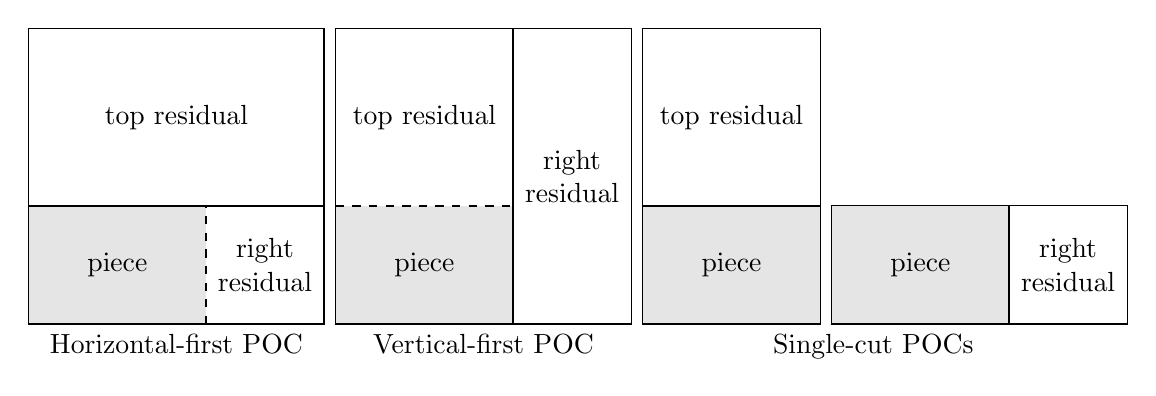
\begin{tikzpicture}[scale=0.15]
\def\piececolor{gray!20}
\def\labelxshift{12.5}
\def\labelyshift{0}
\def\labelfontsize{\normalsize}
\begin{scope}[shift={(0, 0)}] % FIRST ROW
\begin{scope}[shift={(0, 0)}] % FIRST IMAGE

\fill[\piececolor] (0, 0) rectangle +(15, 10);
\draw[thick, black] (0, 10) -- (25, 10);
\draw[dashed, thick, black] (15, 0) -- (15, 10);
\draw (0,0) rectangle +(25, 25);

\node [align=center, font=\labelfontsize\selectfont] at (7.5, 5) {\labelfontsize piece}; %{\labelfontsize piece-sized \\ \labelfontsize plate};
\node [align=center, font=\labelfontsize\selectfont] at (12.5, 17.5) {\labelfontsize top residual};
\node [align=center, font=\labelfontsize\selectfont] at (20, 5) {right\\residual};

\node [below] at (\labelxshift, \labelyshift) {\labelfontsize Horizontal-first POC};
\end{scope}

\begin{scope}[shift={(26, 0)}] % SECOND IMAGE

\fill[\piececolor] (0, 0) rectangle +(15, 10);
\draw[dashed, thick, black] (0, 10) -- (15, 10);
\draw[thick, black] (15, 0) -- (15, 25);
\draw (0,0) rectangle +(25, 25);

\node [align=center, font=\labelfontsize\selectfont] at (7.5, 5) {\labelfontsize piece}; %{\labelfontsize piece-sized \\ \labelfontsize plate};
\node [align=center, font=\labelfontsize\selectfont] at (7.5, 17.5) {\labelfontsize top residual};
\node [align=center, font=\labelfontsize\selectfont] at (20, 12.5) {right\\residual};

\node [below] at (\labelxshift, \labelyshift) {\labelfontsize Vertical-first POC};
\end{scope}

\begin{scope}[shift={(52, 0)}] % THIRD IMAGE

\fill[\piececolor] (0, 0) rectangle +(15, 10);
\draw[thick, black] (0, 10) -- (15, 10);
%\draw[dashed, thick, black] (15, 0) -- (15, 10);
\draw (0,0) rectangle +(15, 25);

\node [align=center, font=\labelfontsize\selectfont] at (7.5, 5) {\labelfontsize piece}; %{\labelfontsize piece-sized \\ \labelfontsize plate};
\node [align=center, font=\labelfontsize\selectfont] at (7.5, 17.5) {\labelfontsize top residual};
\end{scope}

\begin{scope}[shift={(68, 0)}] % FOURTH IMAGE

\fill[\piececolor] (0, 0) rectangle +(15, 10);
%\draw[dashed, thick, black] (0, 10) -- (15, 10);
\draw[thick, black] (15, 0) -- (15, 10);
\draw (0,0) rectangle +(25, 10);

\node [align=center, font=\labelfontsize\selectfont] at (7.5, 5) {\labelfontsize piece}; %{\labelfontsize piece-sized \\ \labelfontsize plate};
\node [align=center, font=\labelfontsize\selectfont] at (20, 5) {right\\residual};
\end{scope}
\node [below, align=center, font=\labelfontsize\selectfont] at (71.5, 0) {\labelfontsize Single-cut POCs};

\end{scope}
\end{tikzpicture}

  \legend{Souce: the author.}
  \label{fig:piece_outlining_cut}
\end{figure}

While a POC constituted by two BGCs may be considered a single decision by a solving method and may be seen as happening in succession, in practice, stage restrictions may change the order a cutting machine performs them.
However, these real-world details do not impact the modelling and will not be discussed in this chapter.
Essentially, each piece type that fits into a plate has two POCs associated with it.
One POC that does the horizontal guillotine cut first and then obtains the piece from the first child plate through a vertical cut (if necessary).
This POC always leaves a \emph{top residual plate} (second child plate of the first cut) and often a \emph{right residual plate} (second child plate of the second cut).
The other POC is the same, except that the vertical cut is done first (i.e., always leaving a right residual and often a top residual plate).
Finally, the piece-sized plate obtained by a POC is the first child plate of the second cut if the second cut exists; otherwise, just the first child plate of the only cut.
The piece-sized plate is either immediately regarded as an obtained piece (already enforcing a rule of the restricted problem) or may be considered waste (e.g., the cutting stock problem often allows piece overproduction).
However, the piece-sized plate is \emph{never} treated as an intermediary plate that could be further cut.

A caveat of the coupled representation mentioned above is that, for some instances of the restricted problem, the number of POCs may be larger than the number of restricted cut positions.
In general, each piece type that fits into a plate has two POCs\footnote{The exception happens when the piece type shares the length or the width with the plate and, consequently, both POCs are equivalent and can be considered the same.} (vertical-first and horizontal-first).
An horizontal (vertical) BGC at a restricted position is shared by all piece types with the same length (width).
However, the main advantage of the coupled representation comes from breaking symmetries, not reducing the number of variables.
%For example, if a stripe of width~\(10\) is obtained by a BGC in the restricted problem, it may be used to obtain a single piece of width~\(10\) and four pieces of width~\(8\), and every permutation in the order of the pieces are obtained from the strip is a symmetry, the POC enforce the width~\(10\) piece is the first to be obtained, and that no other mechanism is necessary to guarantee that the piece will be obtained from such plate.

The POCs are a natural choice for the \emph{restricted} problem but not for the \emph{unrestricted} problem for mostly two main reasons.
The first reason is that, in the restricted problem, each horizontal (vertical) cutting position shares length (width) with at least one piece.
However, in the unrestricted problem, some cutting positions can only be reached by combining many pieces.
The second reason is that the definition of the \emph{restricted} problem guarantees that employing only POCs cannot lead to optimality loss; the same is not true for the unrestricted problem (see \cref{fig:distinctions_restricted_unrestricted}).

\begin{figure}[h]
  \caption{Distinctions between, restricted, position-only restricted, and unrestricted problems.}
  \center
  \usetikzlibrary{patterns}
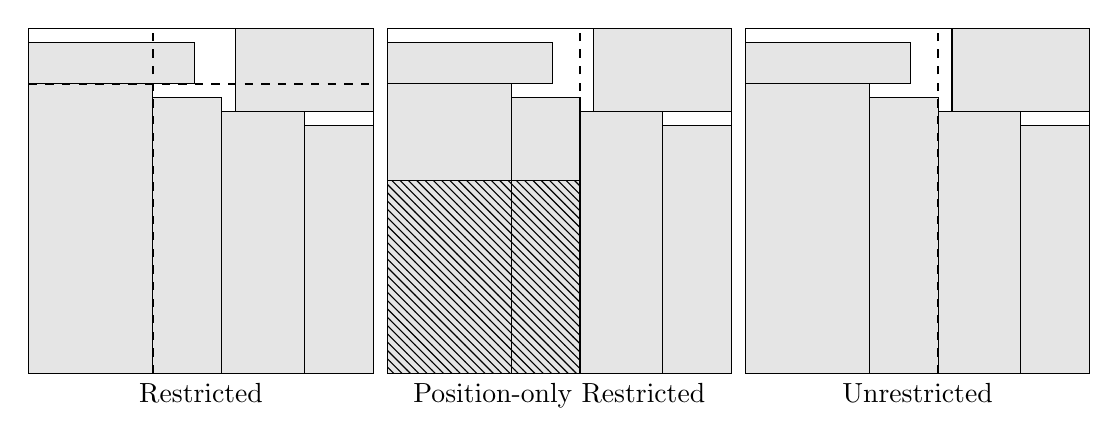
\begin{tikzpicture}[scale=0.175]
\def\piececolor{gray!20}
\def\labelxshift{12.5}
\def\labelyshift{0}
\def\labelfontsize{\normalsize}

\begin{scope}[shift={(0, 0)}] % FIRST ROW
\begin{scope}[shift={(0, 0)}] % FIRST IMAGE
\draw (0,0) rectangle +(25, 25);

%\draw[fill=\piececolor] (0,0) rectangle +(6, 19);
%\draw[fill=\piececolor] (6,0) rectangle +(5, 18);
\draw[fill=\piececolor] (14,0) rectangle +(6, 19);
\draw[fill=\piececolor] (20,0) rectangle +(5, 18);
\draw[fill=\piececolor] (0,0) rectangle +(9, 21);
\draw[fill=\piececolor] (9,0) rectangle +(5, 20);
%\draw[fill=\piececolor] (0,19) rectangle +(10, 6);
\draw[fill=\piececolor] (15,19) rectangle +(10, 6);
\draw[fill=\piececolor] (0,21) rectangle +(12, 3);

\draw[dashed, thick, black] (0, 21) -- (25, 21);
\draw[dashed, thick, black] (9, 0) -- (9, 25);


\node [below] at (\labelxshift, \labelyshift) {\labelfontsize Restricted};


\draw (0,0) rectangle +(25, 25);
\end{scope}

\begin{scope}[shift={(26, 0)}] % SECOND IMAGE
\draw (0,0) rectangle +(25, 25);

%\draw[fill=\piececolor] (0,0) rectangle +(6, 19);
%\draw[fill=\piececolor] (6,0) rectangle +(5, 18);
\draw[fill=\piececolor] (14,0) rectangle +(6, 19);
\draw[fill=\piececolor] (20,0) rectangle +(5, 18);
\draw[fill=\piececolor] (0,0) rectangle +(9, 21);
\draw[fill=\piececolor] (9,0) rectangle +(5, 20);
%\draw[fill=\piececolor] (0,19) rectangle +(10, 6);
\draw[fill=\piececolor] (15,19) rectangle +(10, 6);
\draw[fill=\piececolor] (0,21) rectangle +(12, 3);

\draw[pattern=north west lines] (0,0) rectangle +(14, 14);
\draw[dashed, thick, black] (14, 0) -- (14, 25);

\node [below] at (\labelxshift, \labelyshift) {\labelfontsize Position-only Restricted};
\end{scope}

\begin{scope}[shift={(52, 0)}] % THIRD IMAGE
\draw (0,0) rectangle +(25, 25);

%\draw[fill=\piececolor] (0,0) rectangle +(6, 19);
%\draw[fill=\piececolor] (6,0) rectangle +(5, 18);
\draw[fill=\piececolor] (14,0) rectangle +(6, 19);
\draw[fill=\piececolor] (20,0) rectangle +(5, 18);
\draw[fill=\piececolor] (0,0) rectangle +(9, 21);
\draw[fill=\piececolor] (9,0) rectangle +(5, 20);
%\draw[fill=\piececolor] (0,19) rectangle +(10, 6);
\draw[fill=\piececolor] (15,19) rectangle +(10, 6);
\draw[fill=\piececolor] (0,21) rectangle +(12, 3);

\draw[dashed, thick, black] (14, 0) -- (14, 25);

\node [below] at (\labelxshift, \labelyshift) {\labelfontsize Unrestricted};
\end{scope}

\end{scope}
\end{tikzpicture}

  \legend{
\justifying
The restricted problem cannot obtain the unrestricted optimal solution. If the first cut happens at a restricted position, the child plates cannot fit the six pieces of the optimal solution, regardless of the piece chosen to be obtained first from the original plate and the orientation of the first cut employed. The position-only restricted problem can obtain the unrestricted optimal solution if, by chance, there is an unpacked piece with a width that matches the necessary vertical cut; otherwise, the solution is also out of reach. Source: the author.
}
  \label{fig:distinctions_restricted_unrestricted}
\end{figure}

\citet{silva:2010}~proposes a mathematical formulation for the two-stage and three-stage restricted cutting stock problems.
The formulation was not named by its authors; hence, in this text, it will be referred to as SAV (from the author's surname initials: Silva, Alvelos, and Valério).
The SAV is very similar to the FMT, which is examined in~\cref{sec:furini_model}.
In fact, the SAV may be seen as an FMT variant that uses POCs instead of BGCs.
The limitation to two- and three-stage problems comes from the cut-and-plate enumeration.
If the enumeration is not stopped at a specific stage, the SAV immediately supports unlimited stages.
Essentially, the proposed change is to: hybridise the FMT with the SAV, replacing BGCs with POCs \emph{only} when doing so cannot lead to loss of optimality for the unrestricted problem.
%Next section presents the implementation details for this change.

\section{Implementation details}

As seen in the last section, a POC (\emph{piece-oulining cut}) is prefered over a BGC (\emph{basic guillotine cut}) if it is guaranteed that replacing the latter by the former will not cause loss of optimality.
For the restricted problem, the typical set of horizontal (vertical) cutting positions is just the set of unique values in~\(l_i\) (\(w_i\)) for every piece type~\(i\) that fits into the plate.
Besides one corner case, each single guillotine cut at such positions may be replaced by the corresponding POC.
The corner case arises in cutting positions that come from a length (or width) value shared by two or more pieces.
In this case, a single guillotine cut needs to be replaced by two or more POCs, depending on how many pieces share the corresponding cutting position; otherwise, the model would lose the capability to produce that piece type.

For the unrestricted problem, the exact set of cutting positions often varies between different solving methods.
There are many discretisation procedures (see \cref{sec:enhanced_model}) and reductions to be applied either after or during such discretisations.
The author will focus on the discretisations and reductions procedures employed by the formulations of~\cref{sec:furini_vs_enhanced_comparison} (this is, the FMT and BBA formulations).
The base discretisation employed by both FMT and BBA is straightforward: \(q\) is an horizontal (vertical) cutting position if, and only if, there is a demand-abiding linear combination of lengths (widths) from pieces that fit into the respective plate.
This cutting position set is a superset of the restricted set (from the last paragraph) and will be referred to as the \emph{base unrestricted set}.
Suppose a cutting position allows for the associated BGC to be replaced by (one or more) POCs without loss of optimality for the \emph{unrestricted problem}.
In that case, the cutting position (and, by extension, the BGC) is said to be \emph{replaceable}.
%The set of cutting positions for which the associated single guillotine cuts may be replaced by POCs, without loss of optimality in the context of the \emph{unrestricted problem}, will be referred to as the \emph{replaceable set} henceforth.

A cutting position must meet two conditions to be deemed replaceable.
The first condition is that a cutting position of the same orientation for the same plate exists in the restricted set.
This first condition is necessary because, otherwise, the cut is not outlining a piece, i.e., there is no corresponding piece type to be extracted from the first child plate.
The second condition is that such horizontal (vertical) cutting positions cannot be obtainable by a demand-abiding linear combination of two or more piece lengths (widths), considering only the pieces that fit into the respective plate.
This second condition is necessary because, otherwise, the replaced cut could be necessary for the only optimal cutting pattern of an instance of the unrestricted problem.
An example of this situation can be seen in~\cref{fig:distinctions_restricted_unrestricted} (the middle pattern, i.e., Position-only Restricted).
The middle vertical cut matches a piece width (i.e., it satisfied the first condition); however, if it were replaced by a POC associated with the square piece, it would be impossible to obtain the unrestricted optimal solution (that needs a BGC at the same position).
%the sum of lengths (widths) for a piece multiset in which (a) each piece type multiplity respects the demand, (b) each piece type fits into the first child plate, and (c) the multiset has a cardinality of two or more.
% NOTE: probably we need an image with three diagrams, two of them equal to the introduction ones and a third image showing the possibility of the cut if there is an out-of-the-pattern piece type that has the same size as two other summed.

The two reductions proposed in~\citet{furini:2016}, \emph{Cut-Position} and \emph{Redundant-Cut}, cause little change to the replaceable cutting positions.
Both reductions are briefly described at the start of~\cref{sec:var_enum}.
The only cutting positions removed by \emph{Cut-Position} are the ones not in the restricted set and, therefore, not replaceable.
Moreover, if the cutting position set of a plate is reduced by \emph{Cut-Position} and the kept positions are all replaced with POCs, then that plate and any plate strictly smaller than it will, in fact, be solved by the SAV formulation instead of the FMT formulation.
\emph{Redundant-Cut} may remove a replaceable cutting position.
However, the predicted alternative cutting position from a larger plate will always be replaceable too, and replacing it with one or more POCs never requires adding back the cuts removed by Redundant-Cut.
Also, the BBA formulation never has trim cuts like those removed by Redundant-Cut (see \cref{sec:enhanced_model}), so this enhancement is superseded by it.

BBA adds extraction variables and reduces the base unrestricted set to only the cutting positions up to the midplate.
The extraction variables can be seen as POCs in which both top and right residual plates are guaranteed to be waste; therefore, extractions are not subject to be replaced by POCs.
BBA requires us to differentiate between \emph{binding} and \emph{non-binding} POCs.
A POC is \emph{non-binding} if the piece-sized plate it obtains may be regarded as waste; conversely, if the piece-sized plate must be sold as a piece, then the POC is \emph{binding}.
A \emph{binding} POC cannot be employed if an extra copy of the associated piece type would lead to disrespecting the demand constraint.
If replaceable cuts in the BBA formulation are replaced by \emph{binding} POCs, then there are cases in which loss of optimality occurs.
The cause of this loss of optimality is that, in BBA, a replaceable cut may be required by an optimal solution even if there is no demand for the associated piece.
These seemingly unnecessary cuts aim to reduce the plate size until a large piece can be obtained from the plate through an extraction variable.
A complete example follows.

\begin{example}{Hybridised BBA with binding cuts loses optimality.}
Consider the following G2KP instance: \(L = 100\), \(W = 100\), \(l = [100, 100]\), \(w = [1, 51]\), \(u = [1, 1]\), and \(p = [1, 1]\).
The optimal solution clearly must contain the only available copy of each of the two piece types.
In BBA, there is no cut after the midplate; consequently, a vertical cut at position~\(51\) is ruled out.
The only possibility is a vertical cut at position~\(1\) for which the first child plate could be immediately sold as the single copy of the first piece type.
The second child plate (\(100\)x\(99\)) also does not have an extraction variable for the immediate extraction of the second piece type (\(100\)x\(51\)).
The BBA determines that for an extraction variable to exist ``[...] the plate cannot fit an extra piece (of any type).'' and the first piece type fits together with the second in the \(100\)x\(99\) plate.
Again, a vertical cut at position~\(51\) is unavailable because it happens after midplate.
Consequently, BBA forces the optimal solution to create~\(50\) plates of size~\(100\)x\(1\), one of which will be sold as a piece, and the rest considered waste.
The second child of the~\(50\)th (and last) cut has size~\(100\)x\(50\), and it can be sold as the second piece type because an extraction variable is now available (i.e., the previously quoted condition does not apply anymore).
The adoption of \emph{binding} POCs makes it impossible for BBA to obtain an optimal solution for this example.
The reason is that there are not~\(50\) copies of the first piece type, but these would be needed by the~\(50\) binding piece-outlining cuts necessary to obtain an optimal solution.
The same problem does not arise if the POCs are not binding.
\end{example}

The corner case of two or more pieces sharing the same length/width needs to be considered in the unrestricted problem too, but with a subtle distinction.
In the restricted problem, replacing every single guillotine cut by POCs also brings the advantage of not needing an additional mechanism to enforce the problem definition (i.e., to guarantee piece extractions from the first child plates).
However, in the unrestricted problem, the choice between replacing a single guillotine cut by multiple POCs, or keeping it as a guillotine cut, is just a trade-off between model size and model symmetry.
Therefore, this work further distinguishes between two implementations of hybridisation.
The \emph{conservative} hybridisation substitutes each replaceable horizontal (vertical) BGC with one horizontal-first (vertical-first) POC that is associated with the single piece type that matches the length (width) of the cutting position (and that fits into the respective plate).
If two or more fitting piece types match the cutting position, the conservative hybridisation leaves the BGC unchanged.
The \emph{aggressive} hybridisation substitutes each replaceable horizontal (vertical) BGC with one horizontal-first (vertical-first) POC \emph{for each piece type} that matches its length (width) (and that fits into the respective plate).
%enhancement based on how they deal with the corner case of multiple pieces sharing length or width.
%The distinction between aggressive and conservative is made mostly during cut and plate enumeration, and depending on implementation details, the model formulation may be kept blind to it, i.e., only taking into account which cuts are BGCs and which are POCs.

The author believes it is excessive to present the full formulation and implementation details for every combination of the FMT/BBA formulation with conservative/aggressive hybridisation and binding/non-binding POCs.
The experiments in the next section only consider the BBA with conservative/aggressive hybridisation and non-binding POCs.
The distinction between conservative and aggressive hybridisation is mostly made at the cut and plate enumeration; however, because of an unfortunate notation detail explained further, it is less troublesome to present an accurate formulation of the conservative hybridisation than the aggressive hybridisation.
In light of this, the author chose to fully present the conservative hybridised BBA formulation with non-binding POCs.
The main differences in implementing other combinations are briefly discussed shortly after.

The \emph{conservative hybridised BBA formulation with non-binding} POCs requires a new set of variables, a new set of constraints, a new parameter, and some minor changes to the objective function and some of the existing constraints.
Both the new set of variables and the new set of constraints are bounded by \(|\bar{J}|\) and, therefore, cause only a small relative increase to the model size of a non-trivial instance.
The notation for the new variable and parameter set follows:

\begin{description}
\item [\(s_i\)] \(\forall i \in \bar{J}\) -- Integer variable. Indicates how many piece-sized plates obtained by POCs associated with piece type~\(i\) were sold as pieces of type~\(i\). By \emph{sold} the author means they contributed to the objective function and were accounted for by the demand constraint.
\item [\(h^o_{qji}\)] \(\forall o \in O, j \in J, q \in Q_{jo}, i \in \bar{J}\) -- Binary parameter. Byproduct of the cut and plate enumeration. It has value one if cut~\(x^o_{qj}\) is a POC that produces a piece-sized plate corresponding to piece~\(i\); zero otherwise.%For a cut~\(x^o_{qj}\), \(\sum_{i\in\bar{J}} h^o_{qji}\) is zero if the cut is a BGC, and one if the cut is a POC.
\end{description}

Some variables, parameters, and constraints need just a little reinterpretation or no change at all.
The already established parameter \(a^o_{qkj}\) is exactly the same for BGCs and has a slightly different meaning for POCs.
The difference is that the \(j\) (obtained child plate) is always either the top or right residual (i.e., the POC version of the first and second child) and that both \(o\) (orientation) and \(q\) (cutting position) refer only to the first constituting cut of a POC; the meaning of \(k\) (parent plate) is left unchanged.
The set of variables representing cuts (\(x^o_{qj}\)) also does not need change, as \(h^o_{qji}\) fills the need to identify POCs and their associated piece types. Consequently, the constraints~\eqref{eq:plates_conservation} and~\eqref{eq:just_one_original_plate} presented below are the same as the non-hybridised formulation.

The constraint~\eqref{eq:piece_sized_plates} guarantees each piece-sized plate available~(\(s_i\)) comes from an actual POC.
The remaining changes consist into adding \(s_i\) to the demand constraint~\eqref{eq:hyb_demand} (which avoids overproduction without prohibiting the POCs themselves) and to the objective function~\eqref{eq:hyb_obj} (which allows piece-sized plates to be sold).

% TODO: check if labels are correct

\begin{align}
\bm{max.} &\sum_{(i, j) \in E} p_i e_{ij} + \sum_{i \in \bar{J}} p_i s_i \label{eq:hyb_obj}\\
\bm{s.t.} &\specialcell{\sum_{o \in O}\sum_{q \in Q_{jo}} x^o_{qj} + \sum_{i \in E_{*j}} e_{ij} \leq \sum_{k \in J}\sum_{o \in O}\sum_{q \in Q_{ko}} a^o_{qkj} x^o_{qk} \hspace*{0.05\textwidth} \forall j \in J, j \neq 0,}\tag{\ref{eq:plates_conservation}}\\
	    & \specialcell{\sum_{o \in O}\sum_{q \in Q_{0o}} x^o_{q0} + \sum_{i \in E_{*0}} e_{i0} \leq 1 \hspace*{\fill},}\tag{\ref{eq:just_one_original_plate}}\\
            & \specialcell{s_i \leq \sum_{j \in J}\sum_{o \in O}\sum_{q \in Q_{jo}} h^o_{qji} x^o_{qj} \hspace*{\fill} \forall i \in \bar{J},}\label{eq:piece_sized_plates}\\%\tag{\ref{eq:piece_sized_plates}}\\
            & \specialcell{s_i + \sum_{j \in E_{i*}} e_{ij} \leq u_i \hspace*{\fill} \forall i \in \bar{J},}\label{eq:hyb_demand}\\
	    & \specialcell{x^o_{qj} \in \mathbb{N}^0 \hspace*{\fill} \forall j \in J, o \in O, q \in Q_{jo},}\tag{\ref{eq:trivial_x}}\\
            & \specialcell{e_{ij} \in \mathbb{N}^0 \hspace*{\fill} \forall (i, j) \in E}\tag{\ref{eq:trivial_e}}\\
            & \specialcell{s_{i} \in \mathbb{N}^0 \hspace*{\fill} \forall i \in \bar{J}.}\label{eq:trivial_s}
\end{align}

The aforementioned unfortunate notation detail is the incapability of denoting two or more different cuts~\(x^o_{qj}\) with the same orientation~\(o\) and the same cutting position~\(q\) over the same plate~\(j\).
Therefore, if the aggressive hybridisation replaces a BGC with two or more POCs, then the notation does not allow us to differentiate between them.The~\(a^o_{qkj}\) parameter also needs to change, as it suffers from the same problem.
The aggressive hybridisation code deals with this problem by having unique single indexes for each cut and reverse indexes from each cut property (like orientation or cutting position) to the cuts themselves; this way, the cuts are not limited to the uniqueness of some property combination.

A trivial way to change the presented formulation to use \emph{binding cuts} is to change the constraint set~\eqref{eq:piece_sized_plates} to require equality.
However, the binding cuts can also be implemented without the new variable and constraint sets.
The term \(s_i\) could just be replaced by \(\sum_{j \in J}\sum_{o \in O}\sum_{q \in Q_{jo}} h^o_{qji} x^o_{qj}\) in both the objective function and the demand constraint.
Both mentioned ways to implement binding cuts work on the FMT formulation, which does not have the same loss of optimality problem as the BBA.

% FROM FURINI 2016 PAGE 8: "As an example, if there are three items with widths 21 31 5, the Restricted PP-G2KP Model would allow us to cut at position q = 5 and then perform a further cut at position q = 2 on the obtained plate. Hence, the width of the strip obtained by cutting at position 5 would not correspond to the width of one of the obtained items. For this reason, the Restricted PP-G2KP Model can produce solutions that do not satisfy the definition of restricted guillo- tine cuts given in Section 1."

\section{Experimental results}

In these experiments, for reasons explained further ahead, each instance was solved ten times with ten distinct solver seeds.
The BBA configuration included all applicable reductions previously discussed (i.e., Cut-Position and Plate-Size Normalisation) but excluded initialisation with a primal heuristic and pricing.
The barrier algorithm was used to solve the root node as usual.
Only the Gurobi solver is used in these experiments.
No runs ended in timeout.
The computer setup, as well as the Julia and Gurobi versions/parameters, are the same as described in~\cref{sec:setup_other_formulations}, but the model was built and solved in the same process (i.e., there was no writing and reading from MPS file), and no time limit was enforced.
Three variants are scrutinised: no hybridisation (N. H.), conservative hybridisation (C. H., avoids increasing model size), and aggressive hybridisation (A. H., always hybridise, even if it leads to an increase of the model size).
The first dataset considered is FMT59 (solved as G2KP), and the second is CJCM (solved as G2OPP); more details on these datasets can be found in~\cref{sec:datasets}.

\Cref{tab:g2kp_hyb_summary} shows that both C. H. and A. H. had a similar impact on the total solving time (i.e., a reduction of \(\approx\)20\%).
A. H. had slightly better timings despite the considerable increase in the number of cuts.
C. H. slightly reduces the number of cuts.
Both C. H. and A. H. have almost no effect on the number of plates (or extractions variables).
The percentage of hybridised cuts (\emph{h \%}) and hybridised cuts with just one residual (\emph{k \%}) show that the new reductions changed a very significant part of the models.
The number of instances with the lowest averages shows that N. H. is the best option for most instances.

\begin{table}
\caption{Summary of hybridisation impact over BBA formulation and FMT59 dataset.}
\label{tab:g2kp_hyb_summary}
\begin{center}

\begin{tabular}{lrrrrrrrr}
\hline\hline
\textbf{Variant} & \textbf{T. T.} & \textbf{\(\Delta\) B. T.} & \textbf{\#b} & \textbf{\#extr.} & \textbf{\#cuts} & \textbf{h \%} & \textbf{k \%} & \textbf{\#plates} \\\hline
N. H. & 6,681 & 1,703 & 27 & 186,536 & 2,498,801 & -- & -- & 113,822 \\
C. H. & 5,468 & 489 & 22 & 184,067 & 2,496,421 & 41 & 18 & 113,373 \\
A. H. & 5,447 & 469 & 10 & 184,050 & 3,021,911 & 67 & 28 & 113,366 \\\hline\hline
\end{tabular}
\end{center}

\legend{
\justifying
\emph{T. T.} (Total Time) -- sum of the mean time of all instances, in seconds; \emph{\(\Delta\) B. T.} (Distance from the Best Time) -- sum of the difference in mean time between the respective variant and the variant with the lowest mean time for the same instance, in seconds, i.e., if all variants ran in parallel and had average time, how much time the runs of the respective variant would spend after another thread already finished; \emph{\#b} (best) -- number of instances in which the respective variant had the lowest (best) average time among the variants; \emph{\#extr.} -- total number of extraction variables (considering one model per instance); \emph{\#cuts.} -- total number of cut variables (considering one model per instance); \emph{h \%} -- percentage of \#cuts that were hybridised; \emph{k \%} -- percentage of \#cuts that were not only hybridised but also discarded the second child of the second constituting cut as waste, i.e., the POC resulted in the piece-sized plate and \emph{one} other plate; \emph{\#plates} -- total number of plates (considering one model per instance). Source: the author.
}
\end{table}

A closer look into the data, see \Cref{tab:g2kp_hyb_selected_instances}, reveals that most time difference comes from a few hard instances.
In fact, the instance Hchl4s alone is responsible for most of the difference, with okp2 having about half its relevance and the rest of the instances considerably less impact.
The number of variables hybridised (\emph{H} columns) does not seem a good indicator of how impacted the solving times will be.
However, if N. H. spends most of the time solving the root node (low Non-Root \%), C. H. and A. H. generally do not bring great time improvements.
As the most significant reductions often occur in instances that spend less than 1\% of the time in the root node, the time distribution does not change significantly.
An exception is CHL1s which shows that C. H. seems to impact not the time at the root node but the time at the B\&B, as expected from a symmetry breaking-enhancement.

\begin{table}[!ht]
\caption{Impact of BBA hybridisation in FMT59 instances taking more than 10s.}
\label{tab:g2kp_hyb_selected_instances}
\begin{center}
%\resizebox{!}{.77\height}{%
\begin{tabular}{lrrrrrrrrrrr}
\hline\hline
& \multicolumn{2}{c}{H (\%)} & \multicolumn{3}{c}{Mean Time (s/\%)} & \multicolumn{3}{c}{CV (\%)} & \multicolumn{3}{c}{Non-Root (\%)} \\\cmidrule(lr){2-3}\cmidrule(lr){4-6}\cmidrule(lr){7-9}\cmidrule(lr){10-12}
Inst. & C & A & N (s) & C (\%) & A (\%) & N & C & A & N & C & A \\\hline\hline
Hchl4s & 46 & 57 & 3,657 & 80 & \bestcolumnemph{69} & 76 & 35 & 25 & >99 & >99 & >99 \\
okp2 & 22 & 22 & 1,844 & \bestcolumnemph{77} & 88 & 21 & 19 & 44 & >99 & >99 & >99 \\
Hchl7s & 50 & 77 & 428 & \bestcolumnemph{100} & 134 & 18 & 26 & 19 & 25 & 36 & 44 \\
okp3 & 33 & 49 & \bestcolumnemph{209} & 113 & 122 & 29 & 38 & 35 & >99 & >99 & >99 \\
Hchl8s & 17 & 35 & 253 & 68 & \bestcolumnemph{48} & 73 & 45 & 44 & >99 & >99 & >99 \\
Hchl3s & 46 & 57 & 39 & \bestcolumnemph{93} & 130 & 11 & 21 & 85 & 80 & 82 & 87 \\
Hchl2 & 25 & 77 & 45 & \bestcolumnemph{89} & 144 & 5 & 8 & 18 & 49 & 50 & 65 \\
CHL6 & 45 & 68 & 39 & \bestcolumnemph{91} & 98 & 13 & 15 & 14 & 48 & 46 & 44 \\
CHL7 & 23 & 78 & \bestcolumnemph{30} & 105 & 116 & 8 & 8 & 5 & 26 & 27 & 44 \\
Hchl6s & 51 & 80 & \bestcolumnemph{36} & 103 & 103 & 3 & 5 & 3 & 14 & 18 & 27 \\
CHL1 & 32 & 64 & \bestcolumnemph{26} & 115 & 120 & 14 & 16 & 14 & 68 & 71 & 72 \\
CHL1s & 32 & 64 & 21 & \bestcolumnemph{75} & 121 & 14 & 13 & 6 & 62 & 39 & 61 \\
okp5 & 11 & 12 & 12 & \bestcolumnemph{97} & 99 & 1 & 2 & 2 & 19 & 21 & 21 \\\hline\hline
\end{tabular}
%} % resizebox
\legend{
\justifying
\emph{H (\%)} -- the percentage of all variables (i.e., cut and extraction) that were hybridised for C. H. and A. H.; \emph{Mean Time (s/\%)} -- mean time spent to solve the instance, in seconds for N. H., and in a percentage relative to N. H. for both C. H. and A. H.; \emph{CV} -- coefficient of variation (also known as relative standard deviation) is the standard deviation for N. H., C. H., and A. H., divided by their respective means (CV is always a percentage); \emph{Non-Root (\%)} -- the percentage of the total time which was \emph{not} spent solving the root node. Source: the author.
}
\end{center}
\end{table}

The coefficient of variation of the analysed instances reveals the reason for multiple runs with distinct seeds: the difference between two runs of the same variant but distinct seeds is often larger than the difference between the means of two distinct variants.
Intuitively, breaking symmetries should reduce the variance of the timings.
By cutting symmetric branches, there is less opportunity for a solver seed to traverse multiple equivalent branches with a good relaxation (but bad primal) before finding a primal solution that cuts all such branches.
In fact, when C. H. and A. H. achieve a considerable (20\% or more) reduction of the mean time, the coefficient of variation (which is relative to the mean time) generally shows a reduction.
However, a more general effect, i.e., a higher percentage of model hybridisation (H\%) leading to lower CV (or mean time), is not observed.
Exactly \emph{which} variables were hybridised probably have more impact than \emph{how many} variables.
Finally, the reduction of variance, while positive if the objective is to compare solution methods, may be unwanted when solving the same problem in parallel.
For example, if two methods have similar mean times, the method with the most variance will probably have a thread find the optimal solution first.

The Clautiaux42 dataset has two traits that make it a worst-case scenario for both C. H. and A. H.: most instances are small instances, and the number of pieces sharing the same length, or width, is high.
For the sake of comparison, let us define \(rr_l\) (\(rr_w\)) as the \emph{repeat ratio} of the length (width) values of pieces.
For a given set of piece types, the \(rr_l\) (\(rr_w\)) is a fraction with the difference between the set cardinality and the number of distinct length (width) values as the numerator, and the set cardinality minus one as the denominator.
\emph{Zero} means there is no repetition, and \emph{one} means that all pieces share the same value in the respective dimension.
The FMT59 dataset has \(rr_l \approx 0.178\) and \(rr_w \approx 0.155\), while the Clautiaux42 has \(rr_l \approx 0.465\) and \(rr_w \approx 0.402\).
The metric is a good baseline, even if it does not account for some important details.
For example, small piece types sharing a small length, or width, cause more hybridisation than large pieces sharing a large length (or width).
This last observation is especially true for the BBA formulation, which has no cuts after the midplate.

\Cref{tab:g2opp_hyb_summary} shows that C. H. hybridises only \(\approx\)5\% of the variables and has minimal impact, while A. H. hybridises \(\approx\)55\% of the variables but causes a large increase in both time to solve and the number of cut variables.
\Cref{tab:g2opp_hyb_summary} reveals that for many instances, C. H. has less than 0.5\% of hybridised variables, and the mean and CV show they behave basically the same as N. H. for most instances.
In fact, the slight advantage of C. H. comes from the fact that the two hardest instances have no hybridisation and, therefore, the same mean time as N. H. But the third-hardest instance reaps a few seconds from the hybridisation of 9\% of the variables.
The extra variables from the A. H. have a strong negative effect on the mean time for all instances.
For some instances (such as E05F18 and E00X23), the mean time is more than ten times longer than N. H.
Finally, if rotation is allowed, then \(rr_l\) and \(rr_w\) become a single metric that can only be greater than or equal to both previous values; consequently, the gap in behaviour between C. H. and A. H. can only increase by allowing rotation.

\begin{table}[!ht]
\caption{Summary of hybridisation impact over BBA formulation and Clautiaux42 dataset.}
\label{tab:g2opp_hyb_summary}
\begin{center}
\begin{tabular}{lrrrrrrrr}
\hline\hline
\textbf{Variant} & \textbf{T. T.} & \textbf{\(\Delta\) B. T.} & \textbf{\#b} & \textbf{\#extr.} &\textbf{\#cuts} & \textbf{h \%} & \textbf{k \%} & \textbf{\#plates} \\\hline
N. H. & 255.10 & 11.30 & 32 & 1,205 & 109,369 & 0.00 & 0.00 & 12,642 \\
C. H. & 251.58 & 7.78 & 10 & 1,205 & 109,369 & 5.50 & 2.11 & 12,642 \\
A. H. & 858.30 & 614.50 & 0 & 1,205 & 160,650 & 55.23 & 10.78 & 12,642 \\\hline\hline
\end{tabular}
\end{center}
\legend{The description of the columns can be found in~\Cref{tab:g2kp_hyb_summary}. Source: the author.}
\end{table}

In general, for both datasets, C. H. either had a negligible difference from N. H. or provided some considerable benefit (especially for instances with longer running times).
For solving mostly small instances, or instances with high \(rr_l\) or \(rr_w\), the extra complexity brought to the formulation may not be worthwhile, but the change does not bring much risk of worsening the results.
The A. H. has the best reduction of mean time and CV for both Hchl4s and Hchl8s (FMT59 dataset), but it has a consistently bad performance for small instances with high \(rr_l\) and \(rr_w\).
There is no clear class of instances for which it can consistently outperform C. H. (or N. H.).

\begin{table}[!ht]
\caption{Details of hybridisation impact over BBA formulation and Clautiaux42 dataset.}
\label{tab:g2opp_multiple_seeds_full_CV_hyb}
\begin{center}
%\resizebox{!}{.77\height}{%
\begin{tabular}{lrrrrrrrrrrr}
\hline\hline
& \multicolumn{2}{c}{H (\%)} & \multicolumn{3}{c}{Mean Time (s/\%)} & \multicolumn{3}{c}{CV (\%)} & \multicolumn{3}{c}{Non-Root (\%)} \\\cmidrule(lr){2-3}\cmidrule(lr){4-6}\cmidrule(lr){7-9}\cmidrule(lr){10-12}
Inst. & C & A & N (s) & C (\%) & A (\%) & N & C & A & N & C & A \\\hline\hline
E02F20 & 0 & 58 & \bestcolumnemph{83.70} & 100 & 350 & 62 & 62 & 70 & >99 & >99 & >99 \\
E20F15 & 0 & 54 & \bestcolumnemph{68.26} & 101 & 212 & 51 & 49 & 67 & >99 & >99 & >99 \\
E04F19 & 9 & 57 & 26.59 & \bestcolumnemph{64} & 183 & 117 & 118 & 156 & >99 & >99 & >99 \\
E05F18 & 0 & 57 & \bestcolumnemph{8.52} & 111 & 1,172 & 21 & 17 & 51 & >99 & >99 & >99 \\
E10X15 & 15 & 55 & \bestcolumnemph{7.62} & 124 & 292 & 64 & 28 & 96 & 99 & >99 & >99 \\
E08F15 & 0 & 51 & \bestcolumnemph{5.05} & 115 & 424 & 34 & 33 & 63 & 99 & 99 & >99 \\
E04F17 & 0 & 54 & \bestcolumnemph{4.50} & 100 & 730 & 16 & 16 & 7 & 99 & 99 & >99 \\
E02N20 & 0 & 55 & \bestcolumnemph{4.23} & 100 & 721 & 17 & 17 & 45 & 99 & 99 & >99 \\
E05X15 & 9 & 51 & 3.46 & \bestcolumnemph{92} & 213 & 25 & 25 & 31 & 99 & 99 & 99 \\
E02F17 & 2 & 54 & \bestcolumnemph{3.43} & 111 & 239 & 26 & 17 & 20 & 99 & 99 & >99 \\
E07F15 & 2 & 59 & \bestcolumnemph{3.27} & 121 & 418 & 23 & 28 & 26 & 99 & 99 & >99 \\
E04F20 & 2 & 53 & 2.95 & \bestcolumnemph{76} & 469 & 53 & 43 & 145 & 99 & 98 & >99 \\
E15N15 & 12 & 55 & \bestcolumnemph{2.78} & 123 & 159 & 83 & 77 & 87 & 99 & 99 & 99 \\
E07X15 & 0 & 51 & 2.55 & \bestcolumnemph{99} & 300 & 17 & 18 & 45 & 99 & 98 & 99 \\
E00X23 & 0 & 55 & \bestcolumnemph{2.26} & 100 & 1,237 & 11 & 11 & 100 & 97 & 97 & >99 \\
E03X18 & 0 & 56 & 2.26 & \bestcolumnemph{86} & 310 & 28 & 19 & 40 & 98 & 97 & 99 \\
E04N17 & 9 & 49 & \bestcolumnemph{1.99} & 128 & 234 & 40 & 35 & 31 & 98 & 98 & 99 \\
E03N17 & 2 & 57 & \bestcolumnemph{1.98} & 115 & 236 & 13 & 10 & 18 & 98 & 98 & 99 \\
E04F15 & 1 & 49 & \bestcolumnemph{1.94} & 101 & 182 & 14 & 9 & 13 & 98 & 98 & 99 \\
E03N16 & 1 & 55 & \bestcolumnemph{1.78} & 110 & 337 & 21 & 12 & 19 & 98 & 98 & 99 \\
E02F22 & 4 & 54 & \bestcolumnemph{1.72} & 101 & 321 & 41 & 38 & 55 & 98 & 98 & 99 \\
E04N18 & 0 & 55 & 1.62 & \bestcolumnemph{86} & 743 & 32 & 25 & 48 & 98 & 98 & >99 \\
E05F20 & 10 & 55 & \bestcolumnemph{1.36} & 113 & 243 & 33 & 41 & 45 & 97 & 97 & 98 \\
E00N23 & 0 & 49 & 1.33 & \bestcolumnemph{96} & 215 & 12 & 15 & 22 & 96 & 96 & 98 \\
E08N15 & 8 & 61 & \bestcolumnemph{1.19} & 106 & 436 & 18 & 15 & 29 & 97 & 98 & 99 \\
E05N17 & 0 & 53 & \bestcolumnemph{1.17} & 112 & 364 & 18 & 15 & 52 & 97 & 97 & 99 \\
E05F15 & 11 & 53 & \bestcolumnemph{1.10} & 107 & 386 & 9 & 15 & 24 & 96 & 97 & 99 \\
E15N10 & 13 & 53 & 1.09 & \bestcolumnemph{88} & 236 & 20 & 30 & 24 & 97 & 97 & 98 \\
E03N15 & 9 & 61 & \bestcolumnemph{1.09} & 109 & 249 & 10 & 10 & 22 & 96 & 97 & 98 \\
E05N15 & 1 & 55 & \bestcolumnemph{0.72} & 113 & 200 & 33 & 15 & 21 & 96 & 95 & 97 \\
E20X15 & 0 & 55 & \bestcolumnemph{0.71} & 105 & 531 & 25 & 25 & 45 & 94 & 95 & 99 \\
E07N15 & 8 & 63 & \bestcolumnemph{0.58} & 116 & 313 & 44 & 46 & 105 & 97 & 97 & 98 \\
E04N15 & 19 & 57 & \bestcolumnemph{0.48} & 111 & 350 & 12 & 13 & 20 & 93 & 94 & 97 \\
E13X15 & 0 & 57 & 0.48 & \bestcolumnemph{93} & 205 & 19 & 18 & 19 & 94 & 91 & 96 \\
E13N10 & 13 & 52 & \bestcolumnemph{0.37} & 112 & 164 & 13 & 18 & 14 & 92 & 93 & 95 \\
E00N15 & 1 & 53 & \bestcolumnemph{0.25} & 104 & 134 & 8 & 8 & 11 & 76 & 77 & 83 \\
E13N15 & 5 & 56 & \bestcolumnemph{0.24} & 113 & 787 & 8 & 10 & 25 & 84 & 85 & 97 \\
E07N10 & 32 & 59 & \bestcolumnemph{0.16} & 119 & 158 & 37 & 22 & 13 & 87 & 89 & 88 \\
E10N10 & 21 & 62 & \bestcolumnemph{0.14} & 117 & 218 & 44 & 38 & 15 & 86 & 83 & 90 \\
E10N15 & 29 & 52 & \bestcolumnemph{0.08} & 117 & 148 & 11 & 9 & 8 & 66 & 67 & 73 \\
E03N10 & 11 & 51 & 0.08 & \bestcolumnemph{95} & 166 & 9 & 6 & 8 & 34 & 28 & 76 \\
E00N10 & 31 & 61 & \bestcolumnemph{0.04} & 132 & 199 & 4 & 2 & 109 & 15 & 22 & 61 \\\hline\hline
\end{tabular}
%} % resizebox
\end{center}
\legend{The description of the columns can be found in~\Cref{tab:g2kp_hyb_selected_instances}. Source: the author.}
\end{table}

\chapter{Conclusions}
\label{sec:conclusions}

% Mention rotation (and its improvement)
% A win of symmetry breaking (or more preprocessing)over postprocessing
% Minor things: gurobi slightly advantadge in our context.

% Proof of T instances?

The present work advances the state of the art on MILP formulations for the G2KP \newtext{and related problems}.
\oldtext{This work improved the performance of one of the most competitive MILP formulations for the G2KP by at least one order of magnitude.}
\newtext{This work proposes a (re-)formulation that improves the performance of one of the most competitive MILP formulations for the G2KP by at least one order of magnitude.}
The enhanced formulation dominates the original formulation in the instance set selected by the original formulation.
\oldtext{Concerning other competitive MILP formulations in the literature, the proposed formulation kept the advantage of tighter bounds the original formulation had over them, and greatly reduced the model size and running times for instances that these other formulations had the advantage.}
\newtext{
Concerning other formulations for the problem in the literature, the proposed formulation has shorter run times, and it proves the optimality of more instances (in all datasets in which any of the considered formulations can prove the optimality of at least one instance).
The weakness of the proposed formulation is that in harder datasets (like APT) it will either be unable to solve the root node under the time limit or fail by memory exhaustion.
The other formulations cannot prove the optimality of instances of this dataset either, but they are able to return good solutions at least.
}

\newtext{
The proposed formulation and the plate-size normalisation are enhancements practically exempt from drawbacks except for the extra complexity of implementation, which is still lower than the pricing procedure they mostly supersede. The proposed hybridisation also does not add too much complexity to the implementation. However, it achieves moderate success only in runs where most time is spent after solving the root node, and its aggressive variant risks a large increase to run time for easier instances.
}

\newtext{
The flexibility advantage of formulations allows for easy adaptation for the rotation variant and changing the problem to G2MKP, G2OPP, and G2CSP.
G2MKP is not deeply studied by the literature, and this thesis gives a starting point for future practitioners.
For the G2CSP, as it is common in many CSP variants, a simple formulation has difficulty keeping with the state of the art.
The relaxation upper bound is often optimal, but good upper and lower bounds methods can often prove optimality without needing a systematic framework for exploring the search space.
The formulation can be a tool for scanning through the search space when these bounds cannot close the gap by themselves, but it is not competitive by itself.
For the G2OPP, the proposed formulation seems competitive against a similar approach (a constraint programming model), but it is orders of magnitude slower than the state-of-the-art bottom-up pattern enumeration (which has the disadvantage of needing even more memory than the proposed formulation).
}

\newtext{
In the experiments, some elementary inferences were already discussed, such as the impact on the performance caused by the LP-solving algorithm, the specific changes made, MIP-starting the models, some procedures proposed together with the original model (i.e., pricing and some preprocessing reductions), allowing rotation, and choice of the solver.
The author deemed these too specific to be discussed here and better contextualised in their respective experiment sections.
}
\oldtext{
In the experiments, some elementary inferences were already discussed, for example: the limitations (and partial success) of the improved formulation against the most recent and challenging instances in the literature; and the impact on the performance caused by the LP-solving algorithm, by the specific changes made, by MIP-starting the models, and by some procedures proposed together with the original model (i.e., pricing and some preprocessing reductions).
Here more general conclusions from a broader perspective are presented.
}

\emph{The author believes symmetry-breaking plays a significant part in the success of the proposed formulation.}
In the experiments, the text focuses on the significant reduction of the model size because it is easier to measure.
However, in~\cref{sec:comparison}, by comparing formulations with and without the \emph{purge} procedure, it can be seen that a significant reduction of the model size does not always lead to a significant reduction in running times.
In the case of the variables removed by the \emph{purge} procedure (which could never assume a nonzero value), it seems clear the solver was able to disregard them without the need for the explicit removal by \emph{purge}.
The same does not apply to the variables removed by the enhanced model \newtext{, the plate-size normalisation, the hybridisation, or even the (rotation-specific) mirror-plate enhancement)}, which could assume nonzero values and compose symmetric solutions.
\oldtext{A single extraction variable may replace many distinct sequences of cuts that would extract the same piece from the same slightly-larger plate.}
\newtext{Each of these enhancements either removes redundant variables which could assume non-zero values or change the variables to further restrict the search space (without losing the guarantee of optimality).}
\newtext{The enhanced formulation did not present consistent gains in the LP relaxation for them to be responsible for the observed improvement in performance.}
The author also believes the results suggest that clever dominance rules may considerably improve pseudo-polynomial models (which often have tight bounds but large formulations) before resorting to more complicated techniques (as the pricing procedure proposed in~\citet{furini:2016}\newtext{, and described in~\cref{sec:pricing}}, or column generation techniques).

\oldtext{
\emph{Limited parallelisation of solving LP models is becoming a bottleneck.}
Obtaining tighter bounds, even at the cost of larger model size, is often valuable.
Some recent examples of this trade-off are pseudo-polynomial models like ours, but exponential-sized models solved by column generation are a pervasive and older example of the same trade-off.
In the experiment focusing on finding new optimal solutions for hard instances, it became clear that this approach shifts computational effort from the massively parallelisable B\&B phase to the almost serial root node relaxation phase.
This effect postpones finding the first primal solution and diminishes the value in massive computer clusters.
}

%Our suggestions for future works follow: adapt the formulation for closely related problem variants and compare to their state-of-the-art solving procedure; expand on the symmetry-breaking; \oldtext{search for more parallelisable ways of solving LPs;} consider other frameworks besides the pricing framework of~\citet{furini:2016}.

% TODO: say that one rotation-specific enhancement that was not tested is to take into consideration which length and width are unique to a single piece, so if the width was already used in the discretisation for the same dimension the length cannot be, and vice-versa.

%\chapter{Future Works}
\label{sec:future_works}

For the thesis, we plan to extend the work presented in, at least, two central tracks.
The first track focus on \emph{flexibility}, and the second track focus on \emph{systematization}.

The primary motivation for using a mathematical formulation as the solving method is \emph{flexibility}.
The possibility of adapting a formulation for other problems/variants/cases often stays theoretical and occasionally is materialised and empirically examined.
We intend to adapt the model for the Guillotine 2D version of at least two of the following problems:
the Multiple Knapsack Problem (MKP), the Strip Packing Problem (SPP), the Cutting Stock Problem (CSP), and the Orthogonal Packing Problem (OPP).
For all these problems, we will consider the no-rotation and the rotation variants.
Both the G2MKP and the G2CSP have homogeneous and heterogeneous variants (respectively, if all original plates have the same dimensions, or not).
Adapting to the homogeneous variant is simpler, but the heterogeneous variant is also a possibility.
We will provide details about these adaptations in the next sections.

There is a tension between \emph{systematization} and constraints on scope, time, and number of pages.
The literature on 2D cutting problems grew fast and consistently in the last two decades~\citep{iori:2020}.
Both this tension and this effervescence begot some unfortunate situations that hinder a systematic consideration of the problem instances.
We do believe the thesis we are proposing may be a good place to contribute to this endeavor.
Given a thesis larger scope, and that we are already considering related problems with a general-purpose approach, it would be natural to expand to consider the problem datasets in the literature.
It is common for a dataset proposed for some 2D cutting problem end up being used in other 2D cutting problems (or variants of the same problem).
Also, different solving methods often have difficulty with different instance traits, and it would be interesting to use a general MILP-based method over them.
The comparison could serve as a baseline for the performance of a general method and, more specifically, for future MILP formulations, in many distinct problems.

\section{Formulation adaptations to other problems}
\label{sec:formulation_adaptation}

In this section, we explain how we intend to adapt our enhanced formulation (presented in \cref{sec:enhanced_model}) to each one of the previously mentioned problems and variants.
For the reader's convenience, we replicate our enhanced formulation below\footnote{We have chosen to reproduce the whole formulation with the same numbering.} accompanied by a refresher on how it works and the notation used.
%For the original model, reproduced by us in~\cref{sec:TODO}, \citet{furini:2016} already explains how to adapt the model to the G2SPP and G2CSP.
The sets we employ are the same as before and keep their usual meaning: \(\bar{J}\) -- the set of pieces, \(J \supseteq \bar{J}\) -- the set of all plates, \(O = \{h, v\}\) -- the set of cut orientations (horizontal and vertical), \(Q_{jo}\) -- the sets of positions for which there is a cut of orientation~\(o\) over plate~\(j\) and, finally, \(E\) -- the set of piece extractions.
We also define \(E_{i*} = \{ j : \exists~(i, j) \in E \}\) (which plates may have a copy of~\(i\) extracted from them) and \(E_{*j} = \{i : \exists~(i, j) \in E \}\) (which pieces may be extracted from a plate~\(j\)).

\begin{align*}
\bm{max.} &\sum_{(i, j) \in E} p_i e_{ij} \tag{\ref{eq:objfun}}\\
\bm{s.t.} &\specialcell{\sum_{o \in O}\sum_{q \in Q_{jo}} x^o_{qj} + \sum_{i \in E_{*j}} e_{ij} \leq \sum_{k \in J}\sum_{o \in O}\sum_{q \in Q_{ko}} a^o_{qkj} x^o_{qk} \hspace*{0.05\textwidth} \forall j \in J, j \neq 0,}\tag{\ref{eq:plates_conservation}}\\
%            & \specialcell{\sum_{o \in O}\sum_{q \in Q_{jo}} x^o_{qj} \leq \sum_{k \in J}\sum_{o \in O}\sum_{q \in Q_{ko}} a^o_{qkj} x^o_{qk} \hspace*{\fill} \forall j \in J\setminus\bar{J},}\label{eq:generic_plates_conservation}\\
	    & \specialcell{\sum_{o \in O}\sum_{q \in Q_{0o}} x^o_{q0} + \sum_{i \in E_{*0}} e_{i0} \leq 1 \hspace*{\fill},}\tag{\ref{eq:just_one_original_plate}}\\
            & \specialcell{\sum_{j \in E_{i*}} e_{ij} \leq u_i \hspace*{\fill} \forall i \in \bar{J},}\tag{\ref{eq:demand_limit}}\\
	    % TODO: fix equation below, the forall part is too long and clashes with the long equation in the first line
	    & \specialcell{x^o_{qj} \in \mathbb{N}^0 \hspace*{\fill} \forall j \in J, o \in O, q \in Q_{jo},}\tag{\ref{eq:trivial_x}}\\
            & \specialcell{e_{ij} \in \mathbb{N}^0 \hspace*{\fill} \forall (i, j) \in E.}\tag{\ref{eq:trivial_e}}
\end{align*}

The domain of all variables is the non-negative integers~\eqref{eq:trivial_x}-\eqref{eq:trivial_e}.
The value of a variable~\(e_{ij}\) indicates the number of times a piece~\(i\) was extracted from a  plate~\(j\).
An extraction only occurs if it respects the piece demand~\eqref{eq:demand_limit} (\(u_i\)~is the profit of piece~\(i\)) and, consequently, every extracted piece is taken into account by the objective function~\eqref{eq:objfun} which maximises the total profit (\(p_i\)~is the demand of piece~\(i\)).

The value of a variable~\(x^o_{qj}\) indicates the number of times (distinct instances of) a plate~\(j\) were cut at position \(q\) by a cut with orientation~\(o\).
Both~\eqref{eq:just_one_original_plate} and~\eqref{eq:plates_conservation} handle which plates are available and, therefore, may be further cut or have pieces extracted from them.
The only purpose of \eqref{eq:just_one_original_plate} is to make available one copy of the original plate (i.e., plate zero).
For each other plate type~\(j\), \eqref{eq:plates_conservation} guarantees that, for each copy of~\(j\) utilised for cutting or piece extraction, a copy of \(j\) was previously obtained from a larger plate.
The number of plate~\(j\) copies obtained by a cut at position~\(q\) and orientation~\(o\) over plate~\(k\) is given by~\(a^o_{qkj}\), this listing is a byproduct of the plate enumeration.

Each of the following inner sections considers a different problem or variant.
For the sake of brevity, we do not present all possible combinations -- for the rotation variant, we employ the G2KP, and for the heterogeneous variant, we employ the (no-rotation) G2MKP.
In the thesis, the goal is to have rotation, no-rotation, homogeneous, and heterogeneous variants for each suitable problem.
Finally, we describe the adaptations at a high abstraction level, without excessive optimization, and we are open to suggestions of improvement in such aspect.

\subsection{Adaptation to the rotation variant}

To adapt the formulation for the G2KP to the rotation G2KP, we need only to:

\begin{enumerate}
\item change the piece set~\(\bar{J}\) before we call the enumeration procedure;\label{item:J_change}
\item create a new set~\(P\), which binds the two rotations of every piece;\label{item:P_creation}
\item change the constraint~\eqref{eq:demand_limit} to take into account this new set~\(P\).\label{item:demand_con_change}
\end{enumerate}

The changes mentioned in \cref{item:J_change} consist of adding to \(\bar{J}\) a new piece~\(i^\prime\) for each piece~\(i\) for which~\(\nexists k \in \bar{J} : l_k = w_i~\land~w_k = l_i\), piece~\(i^\prime\) have~\(l_{i^\prime} = w_i\), \(w_{i^\prime} = l_i\), and~\(u_{i^\prime} = u_i\); differently, for each piece~\(i\) for which~\(\exists k \in \bar{J} : l_k = w_i~\land~w_k = l_i\), we change both \(u_i\) and \(u_k\) to the sum of their previous values.

The set~\(P\) mentioned in~\cref{item:P_creation} may be defined as \(P = \{ \{i, k\} \in P : i \in \bar{J}, k \in \bar{J}, l_k = w_i~\land~w_k = l_i\}\). Each element of~\(P\) is a set of two pieces.

Finally, as mentioned in~\cref{item:demand_con_change}, we change

\begin{flalign*}
&& \sum_{j \in E_{i*}} e_{ij} \leq u_i && \forall i \in \bar{J}\tag{\ref{eq:demand_limit}}
%\specialcell{\sum_{j \in E_{i*}} e_{ij} \leq u_i \hspace*{\fill} \forall i \in \bar{J},}\tag{\ref{eq:demand_limit}}
\end{flalign*}

to

\begin{flalign}
&& \sum_{j \in E_{i*}} e_{ij} + \sum_{j \in E_{k*}} e_{kj} \leq u_i && \forall \{i, k\} \in P\label{eq:rotation_demand}
\end{flalign}

\subsection{Adaptation to the Strip Packing Problem and the Orthogonal Packing Problem}

Differently from the other mentioned problems, the G2SPP does not define a \(W\) value a priori, as the problem searches the minimum \(W\) in which it is possible to pack all pieces.
We set \(W\) to a suitable upper bound, and then we can define our original plate (i.e., plate zero) as usual.

One straightforward adaptation, which does not directly alter plate enumeration, consists of the following steps: (i) add dummy pieces of length \(L\) and every normalized width, (ii) have the dummy pieces share the same one-unit demand, (iii) change the objective function to maximize the width of the selected dummy piece and, finally, (iv) change the demand constraint of all non-dummy pieces to be an equality.
However, this adaptation is not ideal.
For example, it introduces symmetries, as the dummy pieces, which simulate the unused width, may appear in the top, bottom, or middle of the pattern.
Therefore we present a better but not so straightforward adaptation, based on \citet{furini:2016}, it consists of the following changes:

\begin{enumerate}
\item \(W\) is set to be one unit greater than a suitable upper bound instead.
\item The original plate is not vertically discretized (\(Q_{0v} = \emptyset\)).
\item The original plate is horizontally discretized on its full extension.
\item The second child of every horizontal cut over the original plate is waste.
\item \label{item:demand_to_equality} The demand constraint \eqref{eq:demand_limit} becomes an equality, i.e., pieces are required.
\item Avoid direct extraction from the original plate, i.e., omit \(\sum_{i \in E_{*0}} e_{i0}\) from \eqref{eq:just_one_original_plate}.
\item The objective function changes from:
\begin{flalign}
\bm{max.} && \sum_{(i, j) \in E} p_i e_{ij} && \tag{\ref{eq:objfun}}
\end{flalign}
to:
\begin{flalign}
\bm{min.} && \sum_{q \in Q_{0h}} q x^h_{q0} &&
\end{flalign}
\end{enumerate}

The adaptation of the formulation for the G2KP to the G2OPP is trivial.
It consists of the \cref{item:demand_to_equality} above and the removal of the objective function.
If the model is feasible, then the solution to the decision problem is true.
Alternatively, we may just replace the objective function \eqref{eq:objfun} by:

\begin{flalign}
\bm{max.} && \sum_{(i, j) \in E} e_{ij} &&
\end{flalign}

In this case, if the upper bound on the optimal solution value goes below~\(\sum_{i\in\bar{J}} u_i\), then the solution to the decision problem is false.

\subsection{Adaptation to Multiple Knapsack Problem (heterogeneous and homogeneous)}

To adapt the formulation for the G2KP to the G2MKP, we need only to change the right-hand side of
\begin{flalign}
&& \sum_{o \in O}\sum_{q \in Q_{0o}} x^o_{q0} + \sum_{i \in E_{*0}} e_{i0} \leq 1 && \tag{\ref{eq:just_one_original_plate}}
\end{flalign}
from one to the number of available original plates.
The adaptation for the heterogeneous variant is not so straightforward.
First, we need to adapt the notation to account for multiple differently-sized original plates.
In our previous notation, the only references to the original plate are to its length~\(L\), its width~\(W\), and to the fact it is the plate zero in~\(J\).
For the sake of simplicity, we assume plate-size normalization is enabled.
We introduce a set~\(K \subseteq J\) for representing the size-normalized original plates, and for each~\(k \in K\) we define its (normalized) length~\(L_k\), its (normalized) width~\(W_k\), and its number of copies available~\(U_k\).
Finally, we avoid modifying the plate enumeration procedure by setting \(L = max\{L_k : k \in K\}\),  \(W = max\{W_k : k \in K\}\), and plate zero to \((L, W)\) (i.e., it is defined in the same way as before, but with the new dummy values).

With the notation and plate enumeration procedure out of the way, the changes to the formulation boil down to replacing~\eqref{eq:just_one_original_plate} by the following constraint set:

\begin{flalign}
&& \sum_{o \in O}\sum_{q \in Q_{ko}} x^o_{qk} + \sum_{i \in E_{*k}} e_{ik} \leq U_k &&  \forall k \in K
\end{flalign}

\subsection{Adaptation to the homogeneous Cutting Stock Problem}

To adapt the formulation for the G2KP to the homogeneous G2CSP, we introduce a new integer variable~\(b\) and make the following changes to the formulation:

\begin{enumerate}
\item Replace the objective function~\eqref{eq:objfun} by \(\bm{min.}~b\).
\item Replace the literal~\(1\) in the right-hand side of~\eqref{eq:just_one_original_plate} by \(b\).
\item The demand constraint \eqref{eq:demand_limit} becomes an equality, i.e., pieces are required.
\end{enumerate}

The adaptation above does not need computing an upper bound on \(b\) (the number of bin necessary), nor does it need an extra constraint to avoid the classic CSP symmetry problem (in which the same number of used bins may be represented in multiple ways).

\section{A systematic approach to instance datasets}

First, let us further detail the reasoning behind our motivation for a systematic consideration of the literature datasets:

\begin{enumerate}
\item A thesis has a larger scope which supports it.
\item The proposed thesis will already approach many problems which share datasets.
\item It provides better understanding of the context in which they were proposed.
\item Delineate for which problems the datasets are adequate or not.
\item Formulations for 2D cutting problems are recent, many datasets have never been solved using this approach.
\end{enumerate}

As we mentioned before, the 2D cutting literature exhibits many situations which complicate a systematic approach.
We enumerate below some of these situations and illustrate them when appropriate.

\begin{enumerate}
\item A work generates instances and does not name them (e.g., \citet{beasley:1985:guillotine,wang:1983,cw:1977}).
\item Two or more papers end up referring to the same previously unnamed instances by different names (e.g., the last instance proposed by~\citet{beasley:1985:guillotine} was referred to as gcut13 by \citet{martello:1998} and as B by \citet{fekete:1997}).
\item A paper combines aggregated datasets from two or more previous papers and end up with the exact same instance by two distinct names (e.g., \citet{furini:2016} takes cgcut2--3 from \citet{dolatabadi:2012} and 2--3 from \citet{hifi:2001}).
\item The articles proposing the datasets are not mentioned but, instead, a link to a (now defunct) instance repository is given (e.g., \citet{hifi:2001}).
\item In some cases, when a paper employs an artificially generated dataset from the literature, it is not clear if the instances are the same (recovered from the prior work authors or a from a repository) or are newly generated instances sampled from the same distribution (e.g., \citet{martello:1998} and \citet{berkey:1987}). If the instances were generate again (with a different seed and, possibly, a different RNG) then, in newer works that take them from a repository, the origin of the instances may be ambiguous (e.g., \citet{alvarez:2009}).
\item In an empirical comparison against prior work, the later work does not execute an experiment using the same instances, which would help a third-person to transitively compare with them, or with the same prior work (e.g., \citet{martin:2020:bottom}).
\item It is not common for an author to list which datasets they are aware of, and then justify their choice of datasets.
\end{enumerate}

The detailed list of datasets presented in~\cref{sec:datasets} was written for this proposal.
We do believe the list of datasets gives many examples which strengthen the case presented in this section for the importance of a systematic approach.
The list of datasets will be expanded in the thesis as, of now, it does not includes classic instances of related problems, nor even all G2KP instances available in the literature.

\section{Other research possibilities}
\label{sec:alternatives}

The previous sections described two research lines we deem most promising, and which we have considered in detail.
In this section, we describe other ideas we have also considered, but not in the same level of detail.
We do not believe it is reasonable to explore all these ideas in the current time frame.
However, they provide additional flexibility for building a plan of action together with the thesis proposal committee.

\begin{description}
\item[VRPSolver]
	``VRPSolver is a Branch-Cut-and-Price based exact solver for vehicle routing and some related problems.'' (\url{https://vrpsolver.math.u-bordeaux.fr/})
	``Extensive experiments on several variants show that the generic solver has an excellent overall performance, in many problems being better than the best specific algorithms. Even some non-VRPs, like bin packing, vector packing and generalized assignment, can be modelled and effectively solved.'' \citep{pessoa:2020}
	We focus on mathematical models mainly because of the flexibility to adapt the solving method to new problems.
	Consequently, it seems reasonable to also consider frameworks which keep this trait, as it is the case of VRPSolver.
	The VRPSolver has impressive results for the 1D-BPP, better than~\citet{delorme:2019} for some datasets.
	\citet{delorme:2019} employs a pseudo-polynomial formulation that, as our enhanced formulation, greatly reduces the size of the model by avoiding enumeration after the half of a bin, while using a strategy different from ours to achieve this effect.
	These positive results raise the question if VRPSolver could not be used to solve the G2KP and if its performance would be on par with our current approach.
	However, as far as we know, VRPSolver has not been used yet to model any geometric 2D problems, which may indicate some limitation.
\item[Matheuristics]
	In~\cref{sec:comparison}, we have seen that, for hard instances, MIP-starting the model with a solution of reasonable quality is positive.
	For the optional pricing procedure~\citet{furini:2016}, which we also include in our experiments, quickly obtaining such solution is essential.
	Often ad hoc heuristics are used for this purpose.
	In our specific case, we choose to use the same ad hoc heuristic used by~\citet{furini:2016} (for both the MIP-start without pricing and with the pricing).
	Considering flexibility is one of our objectives, it should be not necessary to adapt the (or adopt a) heuristic for each problem variant.
	Ideally, the heuristic should be oblivious to the problem and take only a built model as input, or at least, it should take the cutting graph as input, and be oblivious to the changes in the constraints between problem variants.
	Some alternatives to consider include: the common \emph{restricted master heuristic} mentioned by \citet{delorme:2019} or an adaptation similar to the one they use; some variant of the rounding heuristics discussed in~\citet{alvarez:2002:LP}; or using a formulation with the same flexibility and which is faster to obtain good solutions but has looser upper bounds.
\item[Pricing]
	In our current work, we limited ourselves to reproduce the complicated pricing technique proposed by~\citet{furini:2016}, which was proposed together with the formulation we improve.
	After we implemented the pricing technique for the original formulation it was easy to adapt it to our enhanced formulation. However, the technique loses some of its value by doing so, as it does not account for the extraction variables included in the enhanced formulation.
	We do believe there are some alternatives to explore in this vein, as: simplifying the technique above, adapting it to include extractions, executing it in a more granular fashion for each new incumbent solution inside a callback, or adapting other pricing frameworks of the literature.
\item[Symmetries]
	While our enhanced formulation has fewer symmetries than the original one, further work in this topic remains to be done.
	We present here a concrete case of symmetry which affects our enhanced formulation, and one way to deal with it, at the cost of increasing the model size.
	Our formulation considers one cut at a time; consequently, there are many sequences of cuts which lead to the same final result.
	For example, considering all pieces have the same width, we may obtain three pieces of length 10 from a piece of length 70 throught both \(70 \rightarrow 10~60 \rightarrow 10~50 \rightarrow 10~40\) or \(70 \rightarrow 30~40 \rightarrow 10~20 \rightarrow 10~10\).
	To avoid this symmetry one solution is to triple the number of plates by creating three versions of each plate: (i) one which can only be cut vertically, (ii) one which can only be cut horizontally, and (iii) one which can be cut in any orientation.
	Currently, all plates are of the category (iii).
	With the change, the first child of a vertical cut would be a plate of the category (ii), i.e., which could only be cut horizontally. The analogue is valid for horizontal cuts and the category (i). The second child of every cut will be of the category (iii) as this is needed to keep the correctness.
	The sequence \(70 \rightarrow 30~40 \rightarrow 10~20 \rightarrow 10~10\) becomes unattainable, as the first child of length 30 is cut again in the same orientation (and \(40\) cannot be a first child because our formulation does not allow cuts in the second half of the model).
	For more challenging instances, the reduction of symmetries may be worth the increase in the model size.
\end{description}

In the next section we presents our current plan of action.
For this plan, we have only considered the \emph{Metheuristics} research line in addition to the two central tracks previously discussed.

\section{Plan of action}

Finally, we present the tasks necessary for our plan of action, and a schedule for executing them.

\begin{description}
\item[Simpler Adaptations] Both our enhanced formulation and the original formulation of \citet{furini:2016} will be adapted for the G2OPP, the homogeneous G2MKP, and the homogeneous G2CSP. At this point, the pricing will be disabled for all adaptations. The possibility of piece rotation will be enabled for all formulations and variants considered.
\item[Partial Catalogue] The problem instances for the problems described in \emph{Simpler Adaptations} will be catalogued.
\item[Preliminar Experiments] Experiments using the \emph{Simpler Adaptations} and \emph{Partial Catalogue} will be designed and left to run.
\item[Conference Paper] At this point, we would like to write a short paper on the results of the \emph{Preliminar Experiments} and publish it at a conference. The viability of this task will depend upon conference deadlines. The Symposium on Experimental Algorithms (SEA) and the European Symposium on Algorithms (ESA) are among the possibilities considered.
\item[Advanced Adaptations] The G2SPP, the heterogeneous G2MKP, and the heterogeneous G2CSP need deeper changes to the enumeration process. The viability of implementing formulations for the three problems will be analysed. For each problem, we include we will need to catalogue the instances of that problem too.
\item[Alternative Track] While we consider the technical details of adapting the model for more problems in the \emph{Advanced Adaptations}, we will examine the \emph{Matheutistic} possibilities. We may change the chosen alternative track if we identify some serious bottleneck in the time spent to prove the optimality (\emph{Symmetries}), or if the model size is the main obstacle (\emph{VRPSolver} or \emph{Pricing}).
\item[Final Experiments] Experiments using the \emph{Advanced Adaptations} and any modifications of \emph{Alternative Tracks} will be designed and left to run.
\item[Thesis Writing] The text from \emph{Conference Paper} and any results obtained after it will be adapted to the thesis. Any suggestions about the current text made by the thesis proposal committee will be considered.
\end{description}

\begin{table}
\centering
\caption{Provisional schedule for delivering the thesis.}
\begin{tabular}{@{\extracolsep{4pt}}lccccccccc@{}}
\hline\hline
Task & Nov & Dec & Jan & Feb & Mar & Apr & May & Jun & Jul \\\hline
Simpler Adaptations & \checkmark & \checkmark & \checkmark & & & & & & \\
Partial Catalogue & & \checkmark & \checkmark & \checkmark & & & & & \\
Preliminar Experiments & & \checkmark & \checkmark & & & & & & \\
Conference Paper & & & \checkmark & \checkmark & \checkmark & & & & \\
Advanced Adaptations & & & & \checkmark & \checkmark & \checkmark & & & \\
Alternative Tracks & & & & \checkmark & \checkmark & \checkmark & & & \\
Final Experiments & & & & & \checkmark & \checkmark & \checkmark & & \\
Thesis Writing & & & & & & & \checkmark & \checkmark & \checkmark \\\hline\hline
\end{tabular}
\legend{Source: the author.}
\label{tab:prov_schedule}
\end{table}



\bibliographystyle{./infufrgs/inputs/abntex2-alf}
\bibliography{thesis}

\appendix

\chapter{Details on mentioned datasets}
\label{sec:datasets}

The following is a list of every dataset that provided at least one of the instances used in this thesis experiments, as well as the N and T datasets, discussed in~\cref{sec:about_T_instances}.
The list is sorted by the year of the work that proposed the first (if not all) instances of the dataset.

% What to describe about the datasets:
% Order the datasets by the date they were proposed.
% * The paper that proposed the dataset.
% * The oldest paper we know that referred to the instance by their current name.
% * Other names by what the instances were called, if any.
% * If they are artificially generated, how they were generated.
% * If they are not artificially generated, basic info about them (magnitude).
% * For which specific problem variant they were created.
% * Related with the specific variant, if they specify demand or profit.
% * Repositories with it.

\begin{description}
\item [HH] \emph{Proposed in:} \citet{herz:1972} and \citet{hifi:1997} (see details below) \emph{for the} unweighted unconstrained (and, after, constrained) G2KP, and the \emph{first known reference to the name adopted in this work is} \citet{cung:2000}. \emph{Other names:} the proposing paper does not name the unconstrained version and \citet{hifi:1997} call the constrained version of H. \emph{Characteristics: } ``[...], we have considered another instance (denoted H), derived from the instance of \citet{herz:1972}, by adding an upper bound for each piece. The instance is described by \((L, W) = (127, 98)\), \(n = 5\), \(b = (5, 4, 2, 1, 6)\), \(c_i = l_i \times w_i\) and \((l_i, w_i)\), for \(i = 1 \dots 5\), are given by \((21, 13)\), \((36, 17)\), \((54, 20)\), \((24, 27)\) and \((18, 65)\), respectively.'' \citep{hifi:1997}. Their \(b\) is referred to as~\(u\) in this thesis (i.e., piece demand), the analogue is valid for \(c\) and \(p\) (i.e., piece profit).
\item [cgcut1 to cgcut3] \emph{Proposed in} \citet{cw:1977} \emph{for the} G2KP, and the \emph{first known reference to the name adopted in this work here is} \citet{martello:1998}. \emph{Other names:} the instances were numbered as 1--3 by the proposing paper, which is a common approach but often not considered a name, in this case, however, other papers (e.g., \citet{hifi:1997}) and instance repositories (e.g., \url{ftp://cermsem.univ-paris1.fr/pub/CERMSEM/hifi/2Dcutting}) adopted the numbers as names; also, \citet{fayard:1998} refers to cgcut1--2 as CHW1--2, \citet{tschoke:1995} proposes a four-instance unnamed dataset in which instances 1 and 3 are cgcut1 and cgcut3, consequently, cgcut1 and cgcut3 are also called STS1 and STS3 by PackLib\textsuperscript{2} (\url{https://www.ibr.cs.tu-bs.de/alg/packlib/xml/b-autdg-85-xml.shtml}); \citet{velasco:2019} mention a CW4 instance from \citet{cw:1977}, however, the author believes they wanted to refer to the CW4 instance from \citet{fayard:1998} instead. \emph{Characteristics:} The cgcut1--3 are part of a larger semi-artificially generated dataset, but they were the only ones fully described in the body of the original paper and the most commonly adopted by later works. The authors selected the number of pieces (7, 10, and 20, respectively) and the original plate dimensions (15x10, 40x70, and 40x70, respectively). The piece dimensions were obtained by defining selecting a random value in \([1, 0.25\times L \times W]\) to be the piece area, then selecting a random integer value between one and the piece area to be the piece length and, finally, determined the piece width in base of the already defined piece length and the provisional area (rounding the width up, if necessary, i.e., allowing the area to grow instead of shrink). The profit values were obtained by multiplying the area by a random real number between 1 and 3. Finally, the demand vector was handpicked by the authors to best suit their purposes.
\item [wang20] \emph{Proposed in:} \citet{wang:1983} \emph{for the} unweighted G2KP, i.e., waste minization variant, the paper also cover the G2CSP but the instance does not seem to be used for this purpose, and the \emph{first known reference to the name adopted in this work is}~\citet{fekete:1997}. \emph{Other names:} the instance is also referred as W by~\citet{fayard:1998}, however, in \url{ftp://cermsem.univ-paris1.fr/pub/CERMSEM/hifi/2Dcutting/}, W has a different demand vector (which does not seem to affect the optimal objective value). \emph{Characteristics:} The instance is, according to the author, ``a variation of an example presented by \citet{cw:1977}''. The instance is fully described in the proposing paper and reproduced here: \(L = 70\), \(W = 40\), \(l = [11,\) \(12,\) \(14,\) \(17,\) \(18,\) \(21,\) \(23,\) \(24,\) \(24,\) \(25,\) \(27,\) \(32,\) \(34,\) \(35,\) \(36,\) \(37,\) \(38,\) \(39,\) \(41,\) \(43]\), \(w = [19,\) \(21,\) \(23,\) \(9,\) \(29,\) \(31,\) \(33,\) \(15,\) \(15,\) \(16,\) \(17,\) \(22,\) \(24,\) \(25,\) \(26,\) \(27,\) \(28,\) \(29,\) \(30,\) \(31]\), \(u = [4,\) \(3,\) \(4,\) \(1,\) \(3,\) \(3,\) \(3,\) \(1,\) \(2,\) \(4,\) \(2,\) \(2,\) \(2,\) \(2,\) \(1,\) \(1,\) \(1,\) \(1,\) \(1,\) \(1]\).
\item [gcut1 to gcut13] \emph{Proposed in} \citet{beasley:1985:guillotine} \emph{for the} unconstrained G2KP with both a limited and an unlimited number of stages, and the \emph{first known reference to the name adopted in this work here is} \citet{martello:1998}. \emph{Other names:} gcut13 is also referred to as B by \citet{fekete:1997}. \emph{Characteristics: } The profit of each piece is set to their area, as in the unweighted variant, and the demand of each piece was left undefined, as they were developed for an unconstrained variant. In their experiments, \citet{furini:2016} set the demand of each piece to one, and the same is done here (i.e., in the experiments of this work), to allow the comparison with their results. The gcut1--12 instances are artificially generated: the number of sampled pieces is \([10, 20, 30, 50]\) for the first four, middle four, and last four instances; \(L = W\) and they are \(250\) for the first four, \(500\) for the middle four, and \(1000\) for the last four; both piece length and width are sampled from an integer uniform distribution~\([L/4, 3L/4]\). The gcut13 instance is a real-world instance of \(32\) pieces and an original plate of size \(3000\)x\(3000\), fully described in the Table 2 of the original paper. This assimetry is probably the cause many papers select only the gcut1--12 for their experiments. \emph{Online repositories: } PackLib\textsuperscript{2} \url{https://www.ibr.cs.tu-bs.de/alg/packlib/xml/b-autdg-85-xml.shtml}, and ESICUP \url{https://www.euro-online.org/websites/esicup/data-sets/}.
\item[cl\_* (a.k.a. CLASS)] \emph{Proposed in:} \citet{berkey:1987} (first 6 classes with 50 instances each) and \citet{martello:1998} (last 4 classes with 50 instances each) \emph{for the} two-dimensional BPP (non-guillotine) and the \emph{first known reference to the name adopted in this work is} hard to pinpoint, \citet{martello:1998} refer to each new set of 50 instances they propose as classes, and~\citet{boschetti:2003} echoes this when they merge some instance sets from the two previous works together into a single dataset divided into 10 classes, but the name \emph{CLASS} (also adopted by 2DPackLib) seems clearly accidental. \emph{Other names:} in~\cite{alvelos:2009}, the initials of the authors are used for each part of the dataset (BW for the first six classes, and MV for the four last classes), but other names are also possible, as the instance groups were just numbered (using roman numerals) and the individual instances are referred just by their attributes (i.e., cl\_\emph{class}\_\emph{n}\_\emph{seed}, where \(n\) is the total number of pieces). \emph{Characteristics:} each class has 50 instances, these instances can be further divided into five groups, each group has 10 instances sharing the same~\(n \in \{20, 40, 60, 80, 100\}\), all instances inside a group have exactly the same generation parameters except by the random seed. For the first six classes, both the length and the width of the pieces is sampled from an integer uniform distribution~\([1, 10]\) (classes I and II), \([1, 35]\) (classes III and IV), and \([1, 100]\) (classes V and VI), and the original plates are squares of, respectively, 10, 30, 40, 100, 100 (again), and 300 units; for the last 4 classes all original plates are 100x100, and the piece dimensions are drawn from four \emph{types} of piece size distribution. Each piece from the class (originally referred to as)~\(k \in \{I, II, III, V\}\) has 70\% chance of being sampled from the distribution of \emph{type}~\(k\), and 10\% chance from being sampled from each of the other three types. The four \emph{types} of distribution are uniformily random integers. The length (width) range for the types of distribution I to IV are, respectively, \([1, 50]\) (\([66, 100]\)), \([66, 100]\) (\([1, 50]\)), \([50, 100]\) (\([50, 100]\)), and \([1, 50]\) (\([1, 50]\)). \emph{Possible sources of confusion:} In~\citet{berkey:1987}, the term `two-dimensional bin-packing problem' is used to describe what is now commonly referred to as Strip Packing Problem (i.e., packing into an strip that is open ended in one dimension), the term is then adopted for `a special case of packing into finite bins' which is the current meaning of the two-dimensional BPP. Also, in \citet{martello:1998}, \emph{seven} new classes are proposed, however, for this combined dataset only the first four classes (referred to as I, II, III, and IV in that work) are taken and they are referred to as classes VII, VIII, IX, and X in the context of this dataset of 10 classes (because the first six come from~\citet{berkey:1987}). The author believes this can be a source of confusion, as class VII in~\citet{martello:1998} is \emph{not} the class VII in the CLASS dataset.
\item [OF1 and OF2] \emph{Proposed in:} \citet{oliveira:1990} \emph{for the} unweighted G2KP (i.e., waste minization variant), and the \emph{first known reference to the name adopted in this work is} \citet{hifi:2001}. \emph{Other names:} not known, but possible, as the instances were just numbered in the proposing paper. \emph{Characteristics: } The OF1--2 are part of a larger artificially generated dataset, but they were the only ones fully described in the body of the original paper and, as far as the author knows, the only ones adopted by later works. The generation procedure is clever but more complex than usual. Considering this thesis only employs two instances, the author do believe it is better just reproduce them than to describe the whole generation process. Both instances have \(L = 40\), \(W = 70\), and \(n = 10\). The profit of each piece is set to their area. OF1 have \(l = [5, 39, 9, 15, 16, 21, 14, 19, 36, 4]\), \(w = [29, 9, 55, 31, 11, 23, 29, 16, 9, 22]\), and \(u = [1, 4, 1, 1, 2, 3, 4, 3, 2, 2]\). OF2 have \(l = [18, 10, 27, 18, 8, 4, 9, 19, 16, 16]\), \(w = [22, 40, 13, 23, 29, 16, 47, 19, 13, 36]\), and \(u = [2, 1, 3, 2, 4, 1, 1, 4, 2, 4]\).
\item [STS1 to STS4] \emph{Proposed in:} \citet{tschoke:1995} \emph{for the} no-rotation and rotation G2KP, and the \emph{first known reference to the name adopted in this work is} \citet{alvarez:2002:tabu} (STS2 and STS4) and PackLib\textsuperscript{2} (STS1 and STS3). \emph{Other names:} the instances STS1 and STS3 are, in fact, cgcut1 and cgcut2 from \citet{cw:1977}, the instances STS2 and STS4 (which were proposed by \citet{tschoke:1995}) are also called TH1 and TH2 by \citet{fayard:1998}. \emph{Characteristics: } As STS1 and STS3 are cgcut1 and cgcut3 (both already described), this entry will focus exclusively on STS2 and STS4. \citet{tschoke:1995} mention the instances are artifical and fully specified in their appendix, but give no details of the generation procedure. The \(L\), \(W\), and \(n\) of the STS2 and STS4 are, respectively, \([55, 99]\), \([85, 99]\), and \([30, 20]\). \emph{Online repositories:} PackLib\textsuperscript{2} \url{https://www.ibr.cs.tu-bs.de/alg/packlib/instances_problem_type.shtml}.
\item [okp1 to okp5] \emph{Proposed in:} \citet{fekete:1997} \emph{for the} 2KP (i.e., non-guillotine G2KP), and the \emph{first known reference to the name adopted in this work is} the proposing paper. \emph{Other names:} not known and improbable (the instances were named by the proposing paper). \emph{Characteristics: } the instances were artificially generated using the same schema than \citet{beasley:1985:nonguillotine} ``after applying initial reduction''. The ``initial reduction'' seems to consist on a set of rules for reducing the pieces demand to the smallest value which does not affect the optimal objective value. The instances were fully described in the proposing paper. The original plate of all instances is 100x100, and the number of piece types in the five instances are 15, 30, 30, 33, and 29, respectively. The schema is the same as the one described in this list for the cgcut1--3 instances except that (i) the length is picked from~\([1, L]\) (instead of the provisory piece area) and (ii) the demand vector was not handpicked but a random integer among 1, 2, and 3 (which may be changed by the ``initial reduction'', as mentioned above).
\item [A1 to A5] \emph{Proposed in:} \citet{hifi:1997} \emph{for the} weighted and unweighted G2KP (which is referred to as `constrained two-dimensional cutting stock problem' in the paper), and the \emph{first known reference to the name adopted in this work is} the proposing paper. \emph{Other names:} not known and improbable (the instances were named by the proposing papers; but note the similarly named instances A-1 to A-43 from \citet{macedo:2010} have no relation to these instances. \emph{Characteristics: } The instances are fully described in the paper, and their origin (real-world or artificial) is not mentioned. The instances A1 and A2 have arbitrary profits associated to the pieces, the A3, A4, and A5 do not (i.e., the piece area is used). The original plates range from 50x60 to 132x100, the piece demands range from 1 to 4, the average piece area of the first four instances is 699 (i.e., 26x27) and, for the fifth instance, 1107 (33x33).
\item [CW1 to CW11 and CU1 to CU11] \emph{Proposed in:} \citet{fayard:1998} \emph{for the} weighted and unweighted G2KP (CW means \emph{constrained weighted} and CU mean \emph{constrained unweighted}), and the \emph{first known reference to the name adopted in this work is} the proposing paper. \emph{Other names:} not known and improbable (the instances were named by the proposing paper). \emph{Characteristics: } The CW\(i\) and CU\(i\), for \(i = 1, \dots, 11\), share \(L\), \(W\), \(l\), \(w\), and \(u\); only \(p\) is distinct: in the CU instances \(p_i = l_i \times w_i\), and in the CW instances \(p_i\) is a random integer in~\([100, 1000]\); ``the dimensions of the initial plate, the dimensions of the pieces and the number of pieces to cut \(m\) are uniformly taken in the integer intervals \([100, 1000]\), \([0.1 \times L, 0.7 \times W]\) and \([25, 60]\) respectively.'' \citep{fayard:1998}. The pieces demand \(u_i\) were sampled using~\(max\{1, min\{10, random(0, \lfloor L/l_i \rfloor \times \lfloor W/w_i \rfloor)\}\}\). \emph{Online repositories:} 2DPackLIB \url{http://or.dei.unibo.it/library/2dpacklib-2-dimensional-packing-problems-library}, \url{ftp://cermsem.univ-paris1.fr/pub/CERMSEM/hifi/2Dcutting/}.
\item [CHL1 to CHL7] \emph{Proposed in:} \citet{cung:2000} \emph{for the} G2KP, and the \emph{first known reference to the name adopted in this work is} the proposing paper. \emph{Other names: } not known and improbable (the instances were named by the proposing paper). \emph{Characteristics: } ``[\dots] the dimensions \(l_i\) and \(w_i\) of pieces to cut are taken uniformly from the intervals \([0.1L, 0.75L]\) and \([0.1W, 0.75W]\) respectively. The weight associated to a piece \(i\) is computed by \(c_i = \lceil\rho l_i p_i\rceil\), where \(\rho = 1\) for the unweighted case and \(\rho \in [0.25, 0.75]\) for the weighted case. The constraints \(b_i\), for \(i = 1, \dots, n\), have been chosen such that \(b_i = min\{\rho_1, \rho_2\}\), where \(\rho_1 = \lfloor L/l_i \rfloor\lfloor W/w_i \rfloor \) and \(\rho_2\) is a number randomly generated in the interval \([1, 10]\)'' \citep{cung:2000}. Their \(c_i\) is what is referred to as \(p_i\) in this thesis (i.e., piece profit), the same can be said for \(b_i\) and \(u_i\) (i.e., piece demand). The \(L\), \(W\), and \(n\) must be provided, and for CHL1--7 they are \([132,\) \(62,\) \(157,\) \(207,\) \(20,\) \(130,\) \(130]\), \([100,\) \(55,\) \(121,\) \(231,\) \(20,\) \(130,\) \(130]\) and \([30,\) \(10,\) \(15,\) \(15,\) \(10,\) \(30,\) \(35]\), respectively. \emph{Online repositories:} PackLib\textsuperscript{2} \url{https://www.ibr.cs.tu-bs.de/alg/packlib/instances_problem_type.shtml}, \url{ftp://cermsem.univ-paris1.fr/pub/CERMSEM/hifi/2Dcutting/}.
\item [Hchl1, Hchl2, Hchl9, and Hchl3s to Hchl8s] \emph{Proposed in:} \citet{cung:2000} \emph{for the} weighted and unweighted G2KP, and the \emph{first known reference to the name adopted in this work is} the proposing paper. \emph{Other names:} not known and improbable (the instances were named by the proposing paper). \emph{Characteristics: } The generation procedure is the same described in item CHL1--CHL7. The suffix `s' is used to indicate that the pieces have a profit value equal to their area (as in A1s, A2s, 2s, \dots). However, differently of the other suffixed instances, which had an earlier version without the suffix and with an arbitrary profit vector, there does not seem to exist instances Hchl3--Hchl8. The \(L\), \(W\), \(n\) for the instances (in the order they are numbered) are \([130,\) \(130,\) \(127,\) \(127,\) \(205,\) \(253,\) \(263,\) \(49,\) \(65]\), \([130,\) \(130,\) \(98,\) \(98,\) \(223,\) \(244,\) \(241,\) \(20,\) \(76]\), and \([30,\) \(35,\) \(10,\) \(10,\) \(25,\) \(22,\) \(40,\) \(10,\) \(35]\), respectively. \emph{Online repositories:} \url{ftp://cermsem.univ-paris1.fr/pub/CERMSEM/hifi/2Dcutting/}.
\item [A1s, A2s, 2s, 3s, STS2s, STS4s, and CHL1s to CHL4s] \emph{Proposed in:} \citet{cung:2000} \emph{for the} unweighted G2KP, and the \emph{first known reference to the name adopted in this work is} the proposing paper. \emph{Other names:} not known and improbable (the instances were named by the proposing papers), however, in the text pf the original paper there was a single space separating the instance name from the `s' which was supressed by all subsequent works. \emph{Characteristics: } ``The instances 2 s--3 s, A1 s--A2 s, STS2 s--STS4 s and CHL1 s--CHL4 s represent exactly the instances 2--3 , A1--A2, STS2--STS4 and CHL1--CHL4, respectively for which the profit of each piece is represented by its area.''. \citep{cung:2000} The original version of each instance (i.e., without the `s') is described by other items of this list. The instances 2\oldtext{s} and 3\oldtext{s} refer to the alternative name to for the cgcut2 and cgcut3.
\item [T1a to T7e and N1a to N7e] \emph{Proposed in:} \citet{hopper_thesis} \emph{for the} Strip Packing Problem with the guillotine constraint (T instances, but see below) and without the guillotine constraint (N instances), and the \emph{first known reference to the name adopted in this work is} the proposing thesis. \emph{Other names:} not known and improbable (the instances were named by the proposing paper). \emph{Characteristics: } All instances of both datasets have a strip width of 200, and a (supposedly) known optimal height of 200 (with no waste). Each dataset has 35 instances which are divided into categories 1 to 7, each category has five distinct instances indicated by the last character of the instance name: a, b, c, d, e; and these five instances differ from each other only because the seed given to the random number generator. Each category define the same total number of pieces in both datasets, respectively: 17, 25, 29, 49 73, 97, 199. All instances are fully described in the appendix of \citet{hopper_thesis}. The generation procedure is also described by the proposing thesis and consists mostly of starting with a 200x200 plate, and recursively making guillotine cuts to the plates (T instances), or recursively dividing the plates into the five plates of the basic non-guillotinable pattern (N instances). In~\cref{sec:about_T_instances}, a proof by exhaustion shows that T1a is impossible to pack into a guillotine pattern of 200x200, and there is strong evidence empirical evidence of this impossibility for other T instances. The author believes that both dataset T and N were created using the procedure to create non-guillotinable patterns.
\item[C1-p1 to C7-p3] \emph{Proposed in:} \citet{hopper:2001} \emph{for the} Strip Packing Problem (without the guillotine constraint and allowing piece rotation) and the \emph{first known reference to the name adopted in this work is} the proposing paper. \emph{Other names:} while the instances were named by the proposing paper, some papers refer to them by `HT' followed by a number or another identifier\cite{stephane:sat:2010,fleszar:2016}. \emph{Characteristics:} The dataset of 21 instances is divided into categories 1 to 7 (the \emph{C} comes from category) each with problems 1 to 3 (the \emph{p} comes from problem). Each category defines the total number of pieces, a strip width, and the optimal height (known at generation). The number of pieces are 16 or 17 (C1), 25, 28 or 29, 49, 72 or 73, 97, and 196 or 197 (C7). The strip widths are: 20, 40, 60, 60, 60, 80 and 160. The optimal heights are: 20, 15, 30, 60, 90, 120, and 240. Each of the 21 instances is described in its entirety inside the proposing paper. The optimal solution is always a pattern with no waste, and it `` is achieved by packing the rectangles in the order they are stated in the tables using the BLF routine.'' \citep{hopper:2001}. The proposing paper does not give details of the generation process. In this thesis, the experiments show that, for some instances, it is impossible to obtain the known optimal solution while enforcing guillotine cuts and disallowing rotation; however, when rotation is allowed, the optimal solution was found for every instance which the runs did not timeout.
\item [\newtext{APT10 to APT49}] \newtext{\emph{Proposed in:} \citet{alvarez:2002:tabu} \emph{for the} G2KP (unconstrained unweighted and weighted, and constrained weighted and unweighted) and the \emph{Other names:} not known and improbable (the instances were named by the proposing paper). \emph{Characteristics:} The instances APT10 to APT29 are unconstrained, \(L\) and \(W\) are sampled from~\([1500, 3000]\) and the number of pieces types is sampled from~\([30, 60]\). The instances APT30 to APT49 are constrained, \(L\) and \(W\) are sampled from~\([100, 1000]\), the number of pieces types is sampled from~\([25, 60]\), and the demand of each piece~\(i\) comes from~\(min{u^1_i, u^2_i}\) where \(u^1_i = \lfloor L / l_i \rfloor \times \lfloor W / w_i \rfloor\) and \(u^2_i\) is sampled from~\([1, 10]\). For all intances, the piece lengths are sampled from~\([0.05L, 0.4L]\), and the piece widths are sampled from~\([0.05W, 0.4W]\). The instances APT10 to APT19 (unconstrained), as well as APT30 to APT39 (constrained), are unweighted, this is, the profit of each piece is equal to its area. The instances APT20 to APT29, as well as APT40 to APT49, are weighted, and the profit of each piece~\(i\) is sampled from \([0.25l_iw_i, 0.75l_iw_i]\).}
\item [CJCM] \emph{Proposed in:} \citet{clautiaux:2007}, but sometimes misatributted to~\citet{clautiaux:2008}, \emph{for the} ortogonal packing problem (this is, the non-guillotined G2OPP) and the \emph{first known reference to the name adopted in this work is} \citet{cote:2018} which explicitly refer to the dataset as CJCM, some citation styles abbreviate the authors as `CJCM', so there is a previous work that referred to the instances as `the instances from [CJCM08]' \citep{belov2009branch}. \emph{Other names:} the author is also aware of the name `CCM' employed by \citep{fleszar:2016}; as the dataset was not named by its authors and the instances were identified by their three unique attributes (see below) it is possible other names exist. \emph{Characteristics:} Unfortunately, \citet{clautiaux:2007} points to \citet{hopper2002problem} for details on the instance generation method and the author was not able to find a copy of the latter. Besides that reference, the proposing paper tell us that ``The idea is to obtain both feasible and non-feasible problem instances. The first step of the algorithm consists in randomly generating a set of values whose sum is equal to \((1 - \epsilon)WH\). These values are the areas of the items in the created instance. Then the values are factorized to get the width and the height of the items.'' \citep{clautiaux:2007}. In this thesis, the name of individual instances follow the pattern E\(\epsilon f n\), in which \(\epsilon\) are two digits indicating \((LW - \sum_{i \in \bar{J}} l_i w_i u_i)/100\) (i.e., guaranteed waste percentage if feasible), \(f\) is the feasibility status as determined by the methods employed in the proposing paper (`F' for feasible, `N' for unfeasible, and `X' for not solved by any of the three methods employed within the time limit of 15 minutes for each), and \(n\) is the total number of pieces (\(\sum_{i \in \bar{J}} u_i\)). ). The selection criteria for the 42 instances of the dataset is not entirely clear: the distribution of \(n\) in the range \([10, 23]\) seems arbitrary, and instances with the same \(\epsilon\) and \(n\) only exist if \(f\) (assessed by the experiments) is distinct. Consequently, it seems like a larger dataset was first generated, and then 42 instances were selected from it based on the results of the experiments. The original plate dimensions are always 20x20, and the piece types are heterogeneous (\(u_i = 1\) for the vast majority of the piece types, going up to \(u_i = 4\) for five piece types in four distinct instances).
\item[A-1 to A-43] \emph{Proposed in:} \citet{macedo:2010} \emph{for the} two-staged G2CSP and the \emph{first known reference to the name adopted in this work is} the proposing paper. \emph{Other names:} not known and improbable (the instances were named by the proposing paper); but note the similarly named instances A1 to A5 from \citet{hifi:1997} have no relation to these instances. \emph{Characteristics:} ``[...],  two sets of real instances from the furniture industry, set A and [...]'' \citep[p. 7]{macedo:2010}. The instances are highly heterogeneous, and their numbering seem to have no relation with any of their characteristics. The most consistent characteristic are the dimensions of the original plates, which are either 2550x2100 (31 instances), 2750x1220 (11 instances), or 2470x2080 (1 instance). A table summarising their characteristics can be found in the proposing paper. \emph{Online repositories:} 2DPackLib \url{http://or.dei.unibo.it/library/2dpacklib}.
\item [P1\_*, P2\_*, P3\_*, and P4\_*] \emph{Proposed in:} \citet{velasco:2019} \emph{for the} rotation and no-rotation G2KP, and the \emph{first known reference to the name adopted in this work is} the proposing paper. \emph{Other names:} not known and improbable (the instances were named by the proposing papers). \emph{Characteristics: } There is a total of 80 instances, each combination of \(i \in \{1, 2, \dots, 5\}\) \newtext{(random number generator seed)} and \(n \in \{25, 50\}\) for each of the following 8 triples of \emph{class}, \(L\), and \(W\): \((1, 100, 200)\), \((1, 100, 400)\), \((2, 200, 100)\), \((2, 400, 100)\), \((3, 150, 150)\), \((3, 250, 250)\), \((4, 150, 150)\), \((4, 250, 250)\). The instance names follow the pattern P\emph{class}\_\(L\)\_\(W\)\_\(n\)\_\(i\). The pieces of instances with \(n = 25\) are a subset of the pieces in instances with \(n = 50\) (i.e., the `first half'). The piece demands are randomly picked from the integer uniform distribution~\([1, 9]\), and the piece profits are the piece area multiplied by a real number randomly picked from the continuous distribution between \(0.5\) and \(1.5\). The classes 1--3 have piece lenghts randomly picked from the integer uniform distribution~\([5, 40]\), and piece widths from \([10, 80]\). In class 4, half the pieces have their length and width defined in the same way as classes 1--3, and the other half uses \([10, 80]\) for length, and \([5, 40]\) for width, i.e., the distributions are switched between dimensions. \emph{Online repositories:} 2DPackLIB \url{http://or.dei.unibo.it/library/2dpacklib-2-dimensional-packing-problems-library}.
\item [CW*\_M{2, 4, 8}] \emph{Proposed in:} this thesis (but it is a direct adaptation of the CW1--CW11 instances from \citet{fayard:1998}) \emph{for the} G2MKP and the \emph{first known reference to the name adopted in this work is} this thesis (the dataset as a whole may be referred to as CW\_M). \emph{Other names:} none. \emph{Characteristics:} each instance CW\(k\)\_M\(m\) is exactly the same as the original CW\(k\) instance except it has \(m\) original plates available instead of just one. To retain the selection aspect of the problem (i.e., \emph{which} pieces will be packed, not only \emph{how} they will be packed), the author chose to only have a CW\(k\)\_M\(m\) instance if \((\sum_{i \in \bar{J}} l_i w_i u_i) \geq 2 m L W\). This is the reason CW1\_M8 to CW5\_M8 do not exist: each instance from CW1 to CW5 has a summed area of their pieces lower than the summed area of \(2 \times 8\) copies of their respective original plates.
\item [A-*\_M2, A-*\_M4, A-\_M8] \emph{Proposed in:} this thesis (but it is a direct adaptation of the A-1 to A-43 instances from \citet{macedo:2010}) \emph{for the} G2MKP and the \emph{first known reference to the name adopted in this work is} this thesis. \emph{Other names:} none. \emph{Characteristics:} each instance A-\(k\)\_M\(m\) is exactly the same as the original A-\(k\) instance except it has \(m\) original plates available instead of just one. To retain the selection aspect of the problem (i.e., \emph{which} pieces will be packed, not only \emph{how} they will be packed), the author chose to only have a A-\(k\)\_M\(m\) instance if \((\sum_{i \in \bar{J}} l_i w_i u_i) \geq 2 m L W\). The set of instances A-1 to A-43 is very heterogeneous, and the numbering seem to be arbitrary, so this leads to an equally arbitrary subset of them respecting the criteria for \(m \in \{2, 4, 8\}\). For the sake of completeness, the numbers of the original instances that have \(m = 2\) counterparts are: 2, 3, 5, 7, 9, 11--21, 23--29, 31--38, and 40--43 (i.e., 35 of the original 43 instances); of these the following 26 original instances have \(m = 4\) counterparts, they are: 2, 5, 7, 9, 11--16, 18--21, 23--25, 27--29, 32, 33, 35, 38, 40, and 41; and, finally, of these the following 16 original instances have \(m = 8\) counterparts: 2, 9, 11, 14--16, 18--21, 24, 27, 29, 32, 33, and 38. This totalises \(35 + 26 + 16 = 77\) instances in this new dataset.
\item [\newtext{FMT59}] \newtext{\emph{Proposed in:} \citet{furini:2016} (no instance is new so it was not proposed but grouped) \emph{for the} weighted, unweighted, constrained, and unconstrained G2KP and the \emph{first known reference to the name adopted in this work is} this thesis. \emph{Other names:} none. \emph{Characteristics:} the dataset contains 37 unweighted instances and 22 weighted instances (59 in total) and comprises the entirety of some literature datasets as well as subsets of others. Every instance come from another dataset described in this list. The unweighted instances are: W, wang20 \citep{wang:1983},
gcut1 to gcut12 \citep{beasley:1985:guillotine},
OF1, OF2 \citep{oliveira:1990},
A3 to A5 \citep{hifi:1997},
CU1, CU2 \citep{fayard:1998},
2s, 3s, A1s, A2s, STS2s, STS4s, CHL1s, CHL2s, CHL5, CHL6, CHL7, Hchl3s, Hchl4s, Hchl6s, Hchl7s, Hchl8s\citep{cung:2000}.
The weighted instances are:
cgcut1 to cgcut3 \citep{cw:1977},
okp1 to okp5 \citep{fekete:1997},
HH \citep{hifi:1997},
2, 3 \citep{cw:1977},
A1, A2 \citep{hifi:1997},
STS2, STS4, CHL1, CHL2, CW1 to CW3, Hchl2 and Hchl9 \citep{cung:2000}.
The dataset was assembled from an assortment of datasets from the OR library (wang20, gcut1 to gcut12, cgcut1 to cgcut3, okp1 to okp5) and the already mixed dataset employed in~\citet{hifi:2001} (all the remaining instances).
The author do not suggest employing this dataset as it is in future works, unless a comparison with a work that has already employed it is needed.
The reason for this recommendation is that, because the literature adopted different names for the same instances, some instances of the dataset are just duplicates with different names.
This is the case for instances 2 and 3 which are the same as cgcut2 and cgcut3.
Taking into account the literature wang20 and W should be the same instance but the instances obtained by the author have distinct demand values for some of the pieces (all the remaining instance characteristics are the same for all pieces).
The weighted instances A1, A2, 2, 3, STS2, STS4, CHL1, and CHL2 have an unweighted version of themselves in the same dataset; the unweighted alternatives have the same name but are suffixed with an `s'.
}
\item [\newtext{Easy18}] \newtext{A subset of the dataset FMT59 defined in this work. Its purpose is to reduce the number of runs needed before discarding a formulation from further consideration. The dataset contains: cgcut1 to cgcut3, gcut1 to gcut12, OF1, OF2, and wang20. See FMT59 for the origin of each instance, and the rest of the list for a description of their characteristics.}
\end{description}
\end{document}
